% This Japanese translation is based on:
%   Commit b20a7910ef3c02186fd009fb48dd74fa29c04e54
%   Date:   Mon Mar 2 18:22:01 2020 +0100
% The original lines is 4941.
%
% 2021-02-01 RC 0.3
% 2021-02-25 RC 0.4
%   Adobe DocumentCloud => https://documentcloud.adobe.com/link/review?uri=urn:aaid:scds:US:18b0b3f9-6495-42c1-952b-3fac098891f9 
% 2021-08-07 RC 0.5 remove line number, modify list environment
% 2021-08-22 RC 0.6 fix bookmark encoding

\RequirePackage{plautopatch}
\documentclass[%draft,
    9pt, %%%
    % headinclude, footexclude,
    % twoside, % this produces strange margins!
    openright, % for new chapters
    notitlepage,
    % cleardoubleempty,
    % headsepline,
    % pointlessnumbers,
    % bibtotoc, idxtotoc,
  % ]{scrbook}
  dvipdfmx,
  nomag
]{shared/jsbook}
\usepackage[deluxe]{otf} % ja: for improved ja OpenType support

\usepackage{titlesec}
\titleformat{\chapter}[display]
{\normalfont%
    \LARGE% %change this size to your needs for the first line
    \bfseries\sffamily}{\chaptertitlename\ \thechapter}{20pt}{%
    \LARGE %change this size to your needs for the second line
    }
\titlespacing*{\chapter}
  {0pt}{0pt}{20pt}

\usepackage[includeall,
  paperheight = 210mm,
  paperwidth = 148mm,
  top = 5mm, % 5mm
  headsep = 7mm, % 7mm
  textheight = 171mm,
  footskip = 10mm, % 7mm
  outer = 16mm,
  marginparwidth = 0mm,
  marginparsep = 0mm,
  textwidth = 110mm
  % textwidth = 37zw
]{geometry}

\renewcommand{\baselinestretch}{1.1}
\usepackage{setspace}
\newcommand{\codesize}{\fontsize{7.75}{10}\selectfont}

\setcounter{errorcontextlines}{400}

% line breaking tolerances
\tolerance=1000  % usually 200, infinite=10000
% last ditch effort: how much space OK to insert
%   in a line to avoid overfull
\setlength{\emergencystretch}{3em}
\usepackage{morewrites}
\usepackage{ifthen}
\usepackage{changepage}\strictpagecheck
\usepackage{tabularx}
\usepackage{array}
\usepackage{graphicx}
\usepackage{color}
\usepackage{fancyvrb}
\usepackage{verbatim}
\usepackage{amsthm}
\usepackage{endnotes}
% \usepackage{listings} \input{listingdefaults}
% \usepackage{makeidx}
%   \makeindex
%\usepackage[columns=2,columnsep=1em,font=footnotesize,hangindent=0.25em,subindent=0.75em,subsubindent=1.5em,totoc]{idxlayout}
\usepackage{enumerate}
\usepackage{fancybox}
\usepackage{fancyhdr}
\usepackage{multirow}
\usepackage{units}
\usepackage{pdfpages}
% \usepackage{ragged2e} % everysel
\usepackage{mathtools}
\usepackage{placeins}
\usepackage[utf8]{inputenc}
\DeclareUnicodeCharacter{200B}{\hspace{0pt}}
\usepackage[T1]{fontenc}
\usepackage{lmodern}
\usepackage[tocindentauto]{tocstyle}

\PassOptionsToPackage{hyphens}{url}\usepackage[hidelinks]{hyperref}

\usepackage{shared/headingstyle}

\renewcommand{\emph}[1]{\textsf{\textgt{#1}}}
\renewcommand{\bf}{\sf}

% change the font used in table to sf
\let\oldtabular\tabular
\renewcommand{\tabular}{\sf \oldtabular}


%
% make caption font smaller (tip from 
% http://dcwww.camd.dtu.dk/~schiotz/comp/LatexTips/LatexTips.html#captfont)
%
\newcommand{\captionfonts}{\sffamily\footnotesize}

\makeatletter  % Allow the use of @ in command names
\long\def\@makecaption#1#2{%
  % \begin{centering}
  \vskip\abovecaptionskip % space between figure & caption
  \sbox\@tempboxa{{\captionfonts \B{#1\, #2}}}%
  \ifdim \wd\@tempboxa >\hsize
    {\captionfonts \B{#1\, #2}\par}
  \else
    \hbox to\hsize{\hfil\box\@tempboxa\hfil}%
  \fi
  % \end{centering}
  \vskip\belowcaptionskip% space between caption & text
}
\makeatother   % Cancel the effect of \makeatletter


%
% ja: from textbook.cls
%
% set Helvetica as default font for section/chap headings
\newcommand{\headingdefault}{ofu}% AvantGarde; use phvb for helvetical-bold
\newcommand{\headingfont}{%
  \sffamily
}

\def\chapterheadskip{0.5in}

\pagestyle{fancy}

\newlength\headerwidth
\addtolength\headerwidth{\marginparsep}
\addtolength\headerwidth{\marginparwidth}
\fancyheadoffset[RO,LE]{\the\headerwidth}
\fancyfootoffset[RO,LE]{\the\headerwidth}

\newcommand{\newheadings}{
  \def\chaptermark##1{\markboth{第 \thechapter 章 \hskip1zw ##1}{}}
  \def\sectionmark##1{\markright{\thesection \hskip1zw ##1}}
  \fancyhf{}
  \fancyhead[RO]{\sf\rightmark}
  \fancyhead[LE]{\sf\leftmark}
  \fancyfoot{}
  \fancyfoot[LE]{\sf\thepage}
  \fancyfoot[RO]{\sf\thepage}
  \renewcommand{\headrulewidth}{0pt}
}

\newcommand{\appendixheadings}{
  \def\chaptermark##1{\markboth{付録 \thechapter  \hskip1zw ##1}{}}
  \def\sectionmark##1{\markright{\thesection \hskip1zw ##1}}
  \fancyhf{}
  \fancyhead[RO]{\sf\rightmark}
  \fancyhead[LE]{\sf\leftmark}
  \fancyfoot{}
  \fancyfoot[LE]{\sf\thepage}
  \fancyfoot[RO]{\sf\thepage}
  \renewcommand{\headrulewidth}{0pt}
}

\fancypagestyle{headings}{\newheadings}
\fancypagestyle{appendix}{\appendixheadings}
\fancypagestyle{plainhead}{\newheadings}
\fancypagestyle{plainfoot}{\newheadings}
\fancypagestyle{myheadings}{\newheadings}
\fancypagestyle{plain}{\newheadings}

\fancypagestyle{foreword}{
  \def\chaptermark##1{\markboth{##1}{}}
  \def\sectionmark##1{\markright{##1}}
  \fancyhf{}
  \fancyhead[RO]{\sf\rightmark}
  \fancyhead[LE]{\sf\leftmark}
  \fancyfoot{}
  \fancyfoot[LE]{\sf\thepage}
  \fancyfoot[RO]{\sf\thepage}
  \renewcommand{\headrulewidth}{0pt}
}


% ja: to help layout config.
\usepackage{layout}

% \usepackage{titlesec}
% \titleformat{\chapter}[display]
%   {\normalfont\huge\bfseries}{\chaptertitlename\ \thechapter}{20pt}{\Huge}
% \titlespacing*{\chapter}
%   {0pt}{50pt}{40pt}

% Control English and Japanese outputs
% un-comment following for final submission
\newif\ifshoworiginal
\newif\ifshowtrans

% 原文、自動翻訳、校正済み、全部表示
\showoriginaltrue
\showtranstrue

% 校正済日本語のみ表示
\showoriginalfalse
\showtranstrue

% 2020-10-07 added for Overleaf
%\usepackage[utf8]{inputenc}
% 2021-08-20 suppress warnings => NG
%\usepackage{silence}
%\WarningFilter{inputenc}{Unicode character}

% 2021-08-30 mune10, this suppress an inputenc warnings. (99+ => 87), but ToC is getting broken.
%\usepackage[postscript]{ucs}
%\usepackage[utf8x]{inputenc}

% 2020-10-10 igonore inoutenc errors
\nonstopmode


% iPad Air 2 resolution: 1536 x 2048
% 1.3333 ratio (4:3)
% LeeSeshia is 15,73 ? 20,96 cm, ratio 1.332
%%\setlength{\paperwidth}{15.73cm} \setlength{\paperheight}{20.96cm}
%\setlength{\paperwidth}{15.72cm} \setlength{\paperheight}{20.95cm}

% A4 for Japanese version (しばらくは、A4で印刷して校正用する体裁にしたいと思います)
% \setlength{\paperwidth}{21.0cm} \setlength{\paperheight}{29.7cm}
% B5 for Japanese version
%\setlength{\paperwidth}{18.2cm} \setlength{\paperheight}{25.7cm}
% A5
% \setlength{\paperwidth}{14.8cm} \setlength{\paperheight}{21.0cm} %%%
% PC size for Japanese Book
%\setlength{\paperwidth}{18.2cm} \setlength{\paperheight}{23.3cm}

%\typearea{calc} % without BCOR results to a DIV of 8 for 11pt
% \typearea[1cm]{18} % TODO: check if 1 cm is the correct number %%%

% \usepackage{indentfirst}
% \usepackage{bxghost}

% \usepackage{scrlayer-scrpage}
% \setkomafont{pagehead}{\sffamily\upshape\small}
% \setkomafont{pagenumber}{\sffamily\small}

\newif\ifbook
\booktrue % comment out for the print book version %%%
%\booktrue % comment out for the print book version

\ifshoworiginal
\ifbook
\else
\cfoot{\hyperlink{contents}{{\textnormal{Contents}}}}
\fi
\fi
\ifshowtrans
\ifbook
\else
% 2021-08-20 remove ToC link at the bottom
\cfoot{\hyperlink{contents}{{\textnormal{目次}}}}
\fi
\fi

% \usepackage{pslatex} % -- times instead of computer modern, especially for the plain article class

%\usepackage[colorlinks=true,bookmarks=false]{hyperref}
% for Japanese bookmark
\usepackage[unicode]{hyperref}
\usepackage{pxjahyper}
\hypersetup{
  colorlinks=true,
  bookmarks=false,
  bookmarksnumbered
} % ignore the hyperref warning



\usepackage{booktabs}
% \usepackage{graphicx}
% \usepackage{xcolor}
\usepackage{multirow}
% \usepackage{cite}
\usepackage{dirtree}
% \usepackage{pdfpages}
\usepackage{makeidx}
\setcounter{tocdepth}{1}
\makeindex
%\usepackage{showidx} % for index debugging
% For alignment on tableshttps://www.overleaf.com/project/5e60eac5de622d000111102e
\usepackage{dcolumn}
\newcommand{\cc}[1]{\multicolumn{1}{c}{#1}}

\newcommand{\code}[1]{{\small{\texttt{#1}}}}
\newcommand{\codefoot}[1]{{\footnotesize{\texttt{#1}}}}

% fatter TT font
\renewcommand*\ttdefault{txtt}
% another TT, suggested by Alex
% \usepackage{inconsolata}
% \usepackage[T1]{fontenc} % needed as well?

\usepackage[procnames]{listings}

% process Japanese by pdflatex
%%% \usepackage[whole]{bxcjkjatype}

\ifbook
\hypersetup{
  linkcolor  = black,
  citecolor  = black,
  urlcolor   = black,
  colorlinks = black,
  bookmarks=false,
}
\else
\hypersetup{
  linkcolor  = blue,
  citecolor  = blue,
  urlcolor   = blue,
  colorlinks = true,
  bookmarks=true,
}
\fi

% not really used
\newenvironment{comment}
{ \vspace{-0.1in}
  \begin{quotation}
  \noindent
  \small \em
  \rule{\linewidth}{0.5pt}\\
}
{
  \\
  \rule{\linewidth}{0.5pt}
  \end{quotation}
}

\newcommand{\scale}{0.6}%%%

% shared in slides and book

\lstdefinelanguage{chisel}{
  morekeywords={abstract,case,catch,class,def,%
    do,else,extends,false,final,finally,%
    for,if,implicit,import,match,mixin,%
    new,null,object,override,package,%
    private,protected,requires,return,sealed,%
    super,this,throw,trait,true,try,%
    type,val,var,while,with,yield},
  otherkeywords={=>,<-,<\%,<:,>:,\#,@},
  sensitive=true,
  morecomment=[l]{//},
  morecomment=[n]{/*}{*/},
  morestring=[b]",
  morestring=[b]',
  morestring=[b]"""
}

\usepackage{color}
\definecolor{dkgreen}{rgb}{0,0.6,0}
\definecolor{gray}{rgb}{0.6,0.6,0.6}
\definecolor{mauve}{rgb}{0.58,0,0.82}
% \definecolor{lightgray}{rgb}{0.93,0.93,0.93}
\definecolor{lightgray}{rgb}{0.94,0.94,0.94}
% \definecolor{lightgray}{rgb}{0.95,0.95,0.95}

% Default settings for code listings
\ifbook
\lstset{%frame=lines,
  language=chisel,
  frame=single,
  rulecolor=\color{gray},
  backgroundcolor=\color{lightgray},
  aboveskip=4mm,
  belowskip=4mm,
  showstringspaces=false,
  columns=fixed, % basewidth=\mybasewidth,
  basicstyle={\codesize\ttfamily},
  numbers=none,
  numberstyle=\footnotesize,
  % identifierstyle=\color{red},
  breaklines=true,
  breakatwhitespace=true,
  procnamekeys={def, val, var, class, trait, object, extends},
  % procnamestyle=\ttfamily,
  tabsize=2,
  float
}
\else
\lstset{%frame=lines,
  language=chisel,
  aboveskip=3mm,
  belowskip=3mm,
  showstringspaces=false,
  columns=fixed, % basewidth=\mybasewidth,
  basicstyle={\small\ttfamily},
  numbers=none,
  numberstyle=\footnotesize\color{gray},
  % identifierstyle=\color{red},
  keywordstyle=\color{blue},
  commentstyle=\color{dkgreen},
  stringstyle=\color{mauve},
  breaklines=true,
  breakatwhitespace=true,
  procnamekeys={def, val, var, class, trait, object, extends},
  procnamestyle=\ttfamily\color{red},
  tabsize=2,
  float
}
\fi

% \lstnewenvironment{chisel}[1][]
% {\lstset{language=chisel,#1}}
% {}
\lstnewenvironment{chisel}[1][]
  {\noindent\minipage{\linewidth}\vspace{0.5\baselineskip}\lstset{language=chisel,#1}}
  {\endminipage}

% \newcommand{\shortlist}[1]{{\lstinputlisting[nolol]{#1}}}
\newcommand{\shortlistbreakable}[1]{{\lstinputlisting[nolol]{#1}}}
\newcommand{\shortlist}[1]{\noindent\begin{minipage}{\linewidth}\vspace{0.5\baselineskip}\lstinputlisting[nolol]{#1}\end{minipage}}

\newcommand{\longlist}[3]{{\lstinputlisting[basicstyle={\codesize\ttfamily}, float, caption={#2}, label={#3}, frame=tb, captionpos=b]{#1}}}

\newcommand{\verylonglist}[3]{{\lstinputlisting[basicstyle={\codesize\ttfamily}, caption={#2}, label={#3}, frame=tb, captionpos=b]{#1}}}



\newcommand{\todo}[1]{{\emph{TODO: #1}}}
\newcommand{\martin}[1]{{\color{blue} Martin: #1}}
\newcommand{\myref}[2]{\href{#1}{#2}}

\ifbook
\renewcommand{\myref}[2]{{#2}{\footnote{\url{#1}}}}

\renewcommand{\myrefnoref}[2]{#2}
\renewcommand{\myrefrefonly}[1]{\hspace{-2.5mm}\footnote{\url{#1}}}}
\renewcommand{\myrefembed}[2]{{#2}{\par{\footnotesize\url{#1}}}}

% \newcommand{\enref}[2]{{#1}\footnote{[英]\hspace{1mm}\url{#2}}}}
% \newcommand{\jaref}[2]{{#1}\footnote{[日]\hspace{1mm}\url{#2}}}}
% \newcommand{\enjaref}[3]{{#1}\footnote{[英]\hspace{1mm}\url{#2}\par\noindent[日]\hspace{1mm}\url{#3}}}
% \newcommand{\enjarefoneline}[3]{{#1}\footnote{[英]\hspace{1mm}\url{#2}\hspace{2mm}[日]\hspace{1mm}\url{#3}}}
% \newcommand{\jaenref}[4]{{#1}\footnote{[日]\hspace{1mm}\url{#2}}\hspace{-1.25mm}(#3\footnote{[英]\hspace{1mm}\url{#4}})\hspace{-1.5mm}}

\newcommand{\enref}[2]{\emph{#1}}
\newcommand{\jaref}[2]{\emph{#1}}
\newcommand{\enjaref}[3]{\emph{#1}}
\newcommand{\enjarefoneline}[3]{\emph{#1}}
\newcommand{\jaenref}[4]{\emph{#1(#3)\hspace{-0.5zw}}}
\fi

\newcommand{\emptypage}{\null\thispagestyle{empty}\clearpage}

% uncomment following for final submission
\renewcommand{\todo}[1]{}
\renewcommand{\martin}[1]{}

% \ifshowtrans %(校正) % 12/30 mune10 日本語化
% \renewcommand{\bibname}{参考文献}
% \renewcommand{\figurename}{図}
% \renewcommand{\tablename}{表}
\renewcommand{\lstlistingname}{コード}
% \fi

\renewcommand{\usekomafont}[1]{\sffamily\mdseries}
\renewcommand{\CPP}{C\raisebox{0.3ex}{\footnotesize ++}}
\renewcommand{\LChika}{L\hspace{0.1zw}チ\hspace{-0.05zw}カ}
\renewcommand{\footnotexbiased}[1]{\hspace{-0.75zw}\footnote{#1}\hspace{0.5zw}}

\begin{document}

\pagestyle{foreword} %%%




\includepdf{chisel-book-ja/front.pdf}
\thispagestyle{empty}
\clearpage
\emptypage


% \layout % uncomment this to show layout information %%%

\ifbook
\else
\includepdf{chisel-cover.pdf}
\newpage
\thispagestyle{empty}
~
\newpage
\fi

\ifshoworiginal
\begin{flushleft}
\thispagestyle{empty}
\ \\
\vspace{1cm}
{\usekomafont{title}\mdseries\huge Digital Design with Chisel}
\ \\
\vspace{1cm}
{\usekomafont{title}\mdseries\Large Second Edition}
\cleardoublepage
\end{flushleft}
\newpage
\fi

% \ifshowtrans %(校正) % 12/30 mune10 日本語化
% \begin{flushleft}
% \thispagestyle{empty}
% \ \\
% \vspace{1cm}
% {\usekomafont{title}\mdseries\huge Chiselで始めるデジタル回路設計}
% \ \\
% \vspace{0.5cm}
% {\usekomafont{title}\mdseries\Large 第二版(日本語版)}
% \cleardoublepage
% \end{flushleft}
% \newpage
% \fi

\ifshoworiginal
%{\large\itshape Beta Edition}\\
%{\large\itshape martin@jopdesign.com}
%\vspace{10cm} \emph{Version: \today}
\begin{flushleft}
\thispagestyle{empty}
\ \\
\vspace{1cm}
{\usekomafont{title}\Huge Digital Design with Chisel\\
\bigskip
{\usekomafont{title}\huge Second Edition}\\
\bigskip
\bigskip
\bigskip
\bigskip
\bigskip
{\usekomafont{title}\huge Martin Schoeberl}
\medskip\\
}
\fi

\ifshowtrans %(校正) % 12/30 mune10 日本語化
% 2021-01-03 Overleaf syntax error. => add novalidate
%%begin novalidate
%{\large\itshape Beta Edition}\\
%{\large\itshape martin@jopdesign.com}
%\vspace{10cm} \emph{Version: \today}
% \begin{flushleft}
\begin{center}
\thispagestyle{empty}
% \ \\
% \vspace*{4cm}
% %{\usekomafont{title}\Huge Digital Design with Chisel\\
% {\usekomafont{title}\Huge Chisel\,{\huge で\,}始め\hspace{-1mm}る\\[+2mm]
% デジ\hspace{-0.75mm}タ\hspace{-1.25mm}ル回路設計}\\
% \bigskip

% %{\usekomafont{title}\huge Second Edition}\\
% {\usekomafont{title}\large 第二版(日本語版)}\\
% \vspace{7cm}
% %{\usekomafont{title}\huge Martin Schoeberl}
% {\usekomafont{title}\large マーチン・シェーベル 著\\ Chisel 勉強会 訳}
% % \medskip\\
% }
%%end novalidate
\vspace*{20mm}
\hfill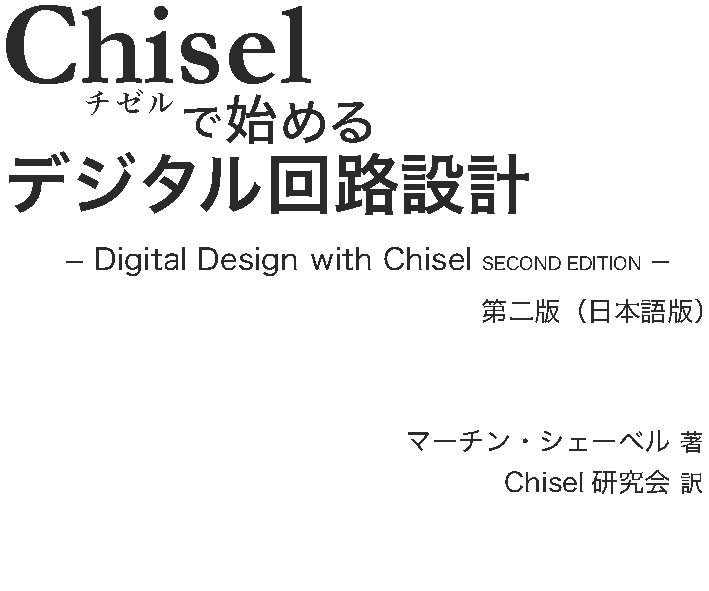
\includegraphics[width=100mm]{chisel-book-ja/inner-front.pdf}
\fi

\newpage
% \end{flushleft}
\end{center}

\thispagestyle{empty}
%\lowertitleback{
%}
\begin{flushleft}
\vspace*{\stretch{1}}
% {\small

% Copyright \copyright{} 2016--2019 Martin Schoeberl
%   \medskip\\
%   \begin{tabular}{lp{.8\textwidth}}
%     \raisebox{-12pt}{\includegraphics[height=18pt]{figures/cc_by_sa}} &
%      This work is licensed under a Creative Commons Attribution-ShareAlike
%      4.0 International License.
%      \url{http://creativecommons.org/licenses/by-sa/4.0/}\\
%   \end{tabular}

% \medskip

% Email: \url{martin@jopdesign.com}\\
% Visit the source at \url{https://github.com/schoeberl/chisel-book}
% \medskip

% Published 2019 by Kindle Direct Publishing,\\
% \url{https://kdp.amazon.com/}

\ifshoworiginal
\medskip
\medskip

\textbf{Library of Congress Cataloging-in-Publication Data}
\medskip

Schoeberl, Martin
\begin{quote}
Digital Design with Chisel\\
Martin Schoeberl\\
Includes bibliographical references and an index.\\
ISBN 9781689336031
\end{quote}

\bigskip

Manufactured in the United States of America.

Typeset by Martin Schoeberl.}
\fi
\end{flushleft}

\frontmatter

% \ifshowtrans % 12/30 mune10 日本語化
% \renewcommand{\contentsname}{目次}
% \fi

% \phantomsection
% \hypertarget{contents}{}
% \tableofcontents

% % \ifshowtrans % 12/30 mune10 日本語化
% % \renewcommand{\listfigurename}{図目次}
% % \renewcommand{\listtablename}{表目次}
\renewcommand{\lstlistlistingname}{コード目次}
% % \fi

% \begingroup
% \let\cleardoublepage\clearpage
% \listoffigures
% \listoftables
% \lstlistoflistings
% \endgroup

\ifshoworiginal
\chapter{Foreword}
\fi
\ifshowtrans %(校正)
\chapter{まえがき} % (校正  初回終了 ========================================================================) RC0.4校正  04/21 HHayashi
\fi

\medskip
\medskip

\ifshoworiginal
It is an exciting time to be in the world of digital design. With the end of Dennard Scaling and the slowing of Moore's Law, there has perhaps never been a greater need for innovation in the field. Semiconductor companies continue to squeeze out every drop of performance they can, but the cost of these improvements has been rising drastically. Chisel reduces this cost by improving productivity. If designers can build more in less time, while amortizing the cost of verification through reuse, companies can spend less on Non-Recurring Engineering (NRE). In addition, both students and individual contributors can innovate more easily on their own.
\fi

\ifshowtrans %(校正 3/5 mune10)
デジタル回路設計の世界で作業することはとてもエキサイティングなことです。
デナードスケーリングの終わりとムーアの法則の減速で、この分野での技術革新が必要となっています。
半導体企業は、依然として性能向上に尽力していますが、性能改善のためのコストが大幅に上昇しています。
Chiselは、デジタル回路設計の生産性を向上させることで、このコストを削減します。
設計の再利用による検証コストの削減や、開発初期投資(Non-Recurring Engineering、NRE)の削減により、設計者はより少ない時間でより多くの(論理)回路を開発することができます。
また、学生や個人でも、イノベーションに取り組むことが簡単にできます。
\fi

\ifshoworiginal
Chisel is unlike most languages in that it is embedded in another programming language, Scala. Fundamentally, Chisel is a library of classes and functions representing the primitives necessary to express synchronous, digital circuits. A Chisel design is really a Scala program that \emph{generates} a circuit as it executes. To many, this may seem counterintuitive: ``Why not just make Chisel a stand-alone language like VHDL or SystemVerilog?'' My answer to this question is as follows: the software world has seen a substantial amount of innovation in design methodology in the past couple of decades. Rather than attempting to adapt these techniques to a new hardware language, we can simply \emph{use} a modern programming language and gain those benefits for free.
\fi

\ifshowtrans %(校正 3/5 mune10, 1/23 2nd)
ChiselはそれがScalaの中に埋め込まれているという点で、他のプログラミング言語とは異なります。
基本的には、同期デジタル回路を表現するために必要なプリミティブを含むクラスと機能をライブラリ化したものが Chisel です。
Chiselのデザインは実際にはScalaのプログラムで、実行可能な回路を\emph{生成}します。
多くの人にとって、これは直感に反するかもしれません: 「なぜ、Chisel をVHDLやSystemVerilogのようなスタンドアロンの言語にしないのだろうか?」
この質問に対する私の答えは次のとおりです。
ソフトウェアの世界では、過去数十年間かつてないほど、様々な設計手法のイノベーションが起こりました。
新しいハードウェアの言語にこれらの技術を適用しなくても、最新のプログラミング言語を \emph{使用する} だけで、これらのメリットを享受することができるのです。
\fi

\ifshoworiginal
A longstanding criticism of Chisel is that it is ``difficult to learn.'' Much of this perception is due to the prevalence of large, complex designs created by experts to solve their own research or commercial needs. When learning a popular language like C++, one does not start by reading the source code of GCC. Rather, there are a plethora of courses, textbooks, and other learning materials that cater toward newcomers. In \emph{Digital Design with Chisel}, Martin has created an important resource for anyone who wishes to learn Chisel.
\fi

\ifshowtrans %(校正 3/5 mune10, 1/23 2nd)
Chiselは、「学ぶことが困難である」と長年批判されてきました。
このような認識の多くは、自身の研究や、商業的なニーズを満足させるために、エキスパートによって作成された大規模で複雑な設計が蔓延したことによるものです。
\CPP のような人気のある言語を学習するとき、人々は GCCのソースコードを読んだりしません。
講座やテキストなど、初習者向けに用意された豊富な学習資料から取りかかります。
Chiselを学びたい人のための重要なリソースとして、この\emph{Chiselで始めるデジタル回路設計}をマーティンは書いてくれました。
\fi

\ifshoworiginal
Martin is an experienced educator, and it shows in the organization of this book. Starting with installation and primitives, he builds the reader's understanding like a building, brick-by-brick. The included exercises are the mortar that solidifies understanding, ensuring that each concept sets in the reader's mind. The book culminates with \emph{hardware generators} like a roof giving the rest of the structure purpose. At the end, the reader is left with the knowledge to build a simple, yet useful design: a RISC processor.
\fi

\ifshowtrans %(校正 3/5 mune10, 1/23 2nd)
マーティンは、経験豊富な教育者であり、それは本書の構成からもみてとれます。
インストールおよび構成要素の解説から始めて、レンガを一つずつ積み上げて建物を作っていくように、読者の理解を深めてゆきます。
付属の演習問題は、理解を固めるための接着剤で、それぞれの概念が読者の心に定着することを助けます。
屋根が家をまとめ上げるのと同じように、\emph{ハードウェアジェネレータ} の理解はこの本の1つの到達点となるでしょう。
最終的には、RISCプロセッサのようなシンプルで有用なデザインを構築するための知識をこの本の読者は得ることになるでしょう。
\fi

\ifshoworiginal
In \emph{Digital Design with Chisel}, Martin has laid a strong foundation for productive digital design. What you build with it is up to you.
\fi

\ifshowtrans %(校正 3/5 mune10)
マーティンは\emph{Chiselで始めるデジタル回路設計}で生産的なデジタル回路設計のための強力なベースを築きました。次に何を作るかはあなた次第です。
\fi

% \medskip
\bigskip %%%
\bigskip %%%

\ifshoworiginal
\noindent Jack Koenig\\
Chisel and FIRRTL Maintainer\\
Staff Engineer, SiFive \\
\fi

\ifshowtrans %(校正 3/5 mune10)
\noindent ジャック・ケーニッヒ\\
ChiselとFIRRTLメンテナ\\
SiFive社 スタッフエンジニア
\fi



\phantomsection
\hypertarget{contents}{}
\tableofcontents

\begingroup
\let\cleardoublepage\clearpage
\listoffigures
\listoftables
\lstlistoflistings
\endgroup



\ifshoworiginal
\chapter{Preface}
\fi
\ifshowtrans %(校正)
\chapter{序文} % (校正  初回終了 ========================================================================) RC0.4校正  04/22 HHayashi
\fi

\ifshoworiginal
% This text goes on the backside of the book, and in Amazon description
This book is an introduction to digital design with the focus on using the hardware construction language Chisel. Chisel brings advances from software engineering, such as object-orientated and functional languages, into digital design.
\fi

\ifshowtrans %(校正 3/6 mune10, 1/23 2nd)
この本では、ハードウェア構築言語であるChiselを使ったデジタル回路設計について解説します。
Chiselは、オブジェクト指向言語や関数型言語など、先進のソフトウェアエンジニアリング技術を、デジタル回路設計の世界にもたらします。
\fi

\ifshoworiginal
This book addresses hardware designers and software engineers. Hardware designers, with knowledge of Verilog or VHDL, can upgrade their productivity with a modern language for their next ASIC or FPGA design. Software engineers, with knowledge of object-oriented and functional programming, can leverage their knowledge to program hardware, for example, FPGA accelerators executing in the cloud.
\fi

\ifshowtrans %(校正 3/6 mune10)
この本は、ハードウェア設計者とソフトウェアエンジニアの両方を対象としています。
VerilogやVHDLの知識を持つハードウェア設計者は、モダンな言語をASICやFPGA設計に活用することで、その生産性を向上させることができます。
オブジェクト指向と関数型プログラミングの知識を持つソフトウェアエンジニアは、例えば、クラウドで稼働するFPGAアクセラレータのようなハードウェアのプログラミング(設計)にその知識を活用することができます。
\fi

\ifshoworiginal
The approach of this book is to present small to medium-sized typical hardware components to explore digital design with Chisel.
\fi

\ifshowtrans %(校正 3/6 mune10)
本書では、小規模もしくは中規模の一般的なハードウェアコンポーネントを例にして、Chiselを使ったデジタル回路設計を紹介していきます。
\fi

% about me, backside

% about me, backside

%Martin Schoeberl is Associate Professor at the Technical University of Denmark, where he is teaching digital electronics and computer architecture. His research interest is on hard real-time systems, time-predictable computer architecture, and real-time Java. He has more than 100 publications in peer reviewed journals, conferences, and books.

%Martin has been four times at UC Berkeley on research stays, where he has picked up Chisel and was in close contact with the developers of Chisel. He lead the research project T-CREST where most of the components have been written in Chisel.

\ifshoworiginal
\section*{Foreword for the Second Edition}
\fi
\ifshowtrans %(校正)
\section*{第二版のまえがき}
\fi

\ifshoworiginal
As Chisel allows agile hardware design, so does open access and on-demand printing
allow agile textbook publishing. Less than 6 months after the first edition of this book
I am able to provide an improved and extended second edition.
\fi

\ifshowtrans %(校正 3/6 mune10)
Chiselは、アジャイルなハードウェア設計を可能にします。同様にオープンアクセスとオンデマンド印刷は、アジャイルな書籍の出版を可能にします。
本書も初版のリリース後、半年未満で改善と拡張を加えた第二版をリリースすることができました。
\fi

\ifshoworiginal
Besides minor fixes, the main changes in the second edition are as follows.
The testing section has been extended. The sequential building blocks chapter contains
more example circuits. A new chapter on input processing explains input synchronization,
shows how to design a debouncing circuit, and how to filter a noisy input signal.
The example designs chapter has been extended to show different implementations of a FIFO.
The FIFO variations also show how to use type parameters and inheritance in digital design.
\fi

\ifshowtrans %(校正 3/6 mune10)
マイナーな修正のほか、第二版での主な変更点は次の通りです。
テストセクションが拡張されています。
順序回路ブロック(sequential building blocks)の章では、より多くの回路例を紹介しています。
入力処理(input processing)に関する新しい章が設けられ、入力の同期、デバウンス回路の設計、そしてノイズが多い入力信号のフィルタリング処理について説明します。
デザイン例の章も拡張され、異なる種類のFIFOの実装方法を説明します。
このFIFOのバリエーションでは、型パラメータと継承をデジタル回路設計のなかでどのように扱うかを解説しています。
\fi

\ifshoworiginal
\section*{Acknowledgements}
\fi
\ifshowtrans %(校正)
\section*{謝辞}
\fi

\ifshoworiginal
I want to thank everyone who has worked on Chisel for creating such
a cool hardware construction language. Chisel is so joyful to use and
therefore worth writing a book about.
I am thankful to the whole Chisel community, which is so welcoming and friendly
and never tired to answer questions on Chisel.
\fi

\ifshowtrans %(校正 3/6 mune10)
クールなハードウェア構築言語であるChiselの開発に携わったすべてのみなさまに感謝します。
Chiselは使用するのがとても楽しく、その本を書く価値があります。
とてもオープンでフレンドリで、Chiselに関する質問に熱心に答えてくれる Chiselコミュニティ全体に感謝しています。
\fi

\ifshoworiginal
I would also like to thank my students in the last years of an advanced computer
architecture course where most of them picked up Chisel for the final project.
Thank you for moving out of your comfort zone and taking up the journey of
learning and using a bleeding-edge hardware description language.
Many of your questions have helped to shape this book.
\fi

\ifshowtrans %(校正 3/6 mune10)
また、最後の数年間、先進コンピュータアーキテクチャコースを受講した学生たちに感謝したいと思います。
ほとんどの生徒が最終プロジェクトのためにChiselを取り上げてくれました。
殻から抜け出し、新しい勉強の旅に出て、最先端のハードウェア記述言語を使用していただき感謝します。
あなたたちの質問の多くは、この本を形作るのに大変役立ちました。
\fi

\ifshowtrans %(日本語版追記)
\clearpage
\section*{日本語訳について}

この日本語訳の作成は Chisel勉強会で行っています。
本書の校正にはRISC-V勉強会も含めて多くの方に助けていただきました。この場を借りてお礼申し上げます。
日本語版のソースコードはこちら{\small\url{https://github.com/chisel-jp/chisel-book}}で公開しています。
翻訳で用いたオリジナルのバーションは『2020年3月2日 b20a791』です。
Githubの方ではオリジナルの更新に合わせて翻訳も新しくしていく予定です。
誤訳や表現の誤りの訂正、改善箇所などありましたら、GhithubでPRを出していただくか、Chisel勉強会のSlackで指摘していただけると助かります。
Chiselに興味ある方は、Chisel勉強会に自由に参加できます。
Chisel勉強会のSlackへ登録はこちら{\small\url{https://chisel-jp-slackin.herokuapp.com/}}からお願いします。

\subsection*{日本語版での変更点}

% 最後の2つについては体裁が代わるため書籍版では修正の必要があります。
\begin{itemize}
    \item 原書の「デジタルデザイン」は、日本語版ではより具体的に「デジタル回路設計」としました。
    \item 日本語の参考文献の追加
    \item 日本語索引の追加
    \item ソースコードのリストに薄いグレーの背景色を設定しました。
    %%% 書籍版では体裁が異なるのでコメントアウトしました。
    % \item また、コード目次に列挙されるソースコードにつきましては、挿入される位置が本文とはずれるため、枠と行番号を追加することで本文中のソースコードと区別しやすいように変更しました。
    % \item Wikipediaへのリンクは(英語)(日本語)の併記としました。これは日本語版Wikipediaの記述が不十分な用語があるためです。
\end{itemize}

% V1.0になったのでRCの履歴はコメントアウトとします
%\subsection*{日本語版の履歴}
%\begin{description}
%\item[2020-10-10] 一時公開版
%\item[2021-02-01] RC 0.3 初回校正版、(目次にLatexソースの行番号追記)
%\item[2021-02-25] RC 0.4 RISCV勉強会校正版
%\item[2021-08-07] RC 0.5 行番号削除、リスト環境を変更
%\item[2021-08-22] RC 0.6 しおりの文字化け修正, A4、B5、PC版に対応
%\item[2021-09-13] RC 0.7 校正
%\item[2021-10-18] RC 0.8 校正
%\item[2021-10-18] v1.0
%\end{description}


\fi %(日本語版追記)

\mainmatter

\pagestyle{plain}

\ifshoworiginal
\chapter{Introduction}
\fi
\ifshowtrans %(校正)
\chapter{はじめに} % (校正  第1章 初回終了 =================================================================) RC0.4校正  04/22, 30 HHayashi
\fi

\label{sec:intro}

\ifshoworiginal
This book is an introduction to digital system design using a modern hardware
construction language, \myref{https://www.chisel-lang.org/}{Chisel}~\cite{chisel:dac2012}.
In this book, we focus on a higher abstraction level than usual in digital design books,
to enable you to build more complex, interacting digital systems in a shorter time.
\fi

\ifshowtrans %(校正 3/6 mune10)
本書は、現代的なハードウェア構築言語である \myref{https://www.chisel-lang.org/}{Chisel}~\cite{chisel:dac2012} を使ったデジタルシステム設計について解説します。
本書では、一般的なデジタル回路設計の書籍に比べ、より高い抽象レベルでの設計に注目し、より複雑で、相互作用のあるデジタルシステムを短期間で開発できるようになることを目指します。
\fi

\ifshoworiginal
This book and Chisel are targeting two groups of developers:
(1) hardware designers and (2) software programmers.
Hardware designers who are fluid in VHDL or Verilog and using other languages such as Python,
Java, or Tcl to generate hardware can move to a single hardware construction language
where hardware generation is part of the language.
Software programmers may become interested in hardware design,
e.g., as future chips from Intel will include programmable hardware to speed up programs.
It is perfectly fine to use Chisel as your first hardware description language.
\fi

\ifshowtrans %(校正 3/6 mune10)
本書およびChiselは、(1) ハードウェア設計者と (2) ソフトウェアプログラマの2つの開発者のグループを対象としています。
VHDLやVerilogになれたハードウェア設計者は、Python、Java、またはTclのような言語も使いこなしながらハードウェアの開発を進めますが、今後はハードウェアの生成が言語の機能の一部となっている単一のハードウェア構築言語を使って開発を進めることができます。
ハードウェア設計にも興味がある(例えば、インテルが性能向上のためにFPGAを将来チップに取り込むために)ソフトウェアプログラマにとっては、
最初に覚えるハードウェア記述言語としてChiselは最適です。
\fi

\ifshoworiginal
Chisel brings advances in software engineering, such as object-orientated
and functional languages, into digital design.
Chisel does not only allow to express hardware at the register-transfer level
but allows you to write hardware generators.
\fi

\ifshowtrans %(校正 3/9 mune10)
Chiselは、オブジェクト指向や関数型言語といったソフトウェア工学の進歩をデジタル回路設計の世界にもちこみます。
Chiselは、レジスタ転送レベル(RTL)でのハードウェア記述をサポートするだけではなく、ハードウェアジェネレータ(生成器)を記述できます。
\fi

\ifshoworiginal
Hardware is now commonly described with a hardware description language.
The time of drawing hardware components, even with CAD tools, is
over. Some high-level schematics can give an overview of the system but are
not intended to describe the system.
The two most common hardware description languages are Verilog and VHDL.
Both languages are old, contain many legacies, and have a moving line of what
constructs of the language are synthesizable to hardware.
Do not get me wrong: VHDL and Verilog are perfectly able to describe a hardware
block that can be synthesized into an
\myref{https://en.wikipedia.org/wiki/Application-specific_integrated_circuit}{ASIC}.
For hardware design in Chisel, Verilog serves as an intermediate language
for testing and synthesis.
\fi

\ifshowtrans %(校正 3/9 mune10)
現在、ハードウェアの設計はハードウェア記述言語(HDL)を使うのが一般的です。
CADツールなどを使用して、お絵かきでハードウェアコンポーネントを設計する時代は終わりました。
回路構成図を作ることはありますが、それはシステムの概要を示すためで、システムを記述するためのものではありません。
最も一般的なハードウェア記述言語は、VerilogとVHDLの2つです。
どちらの言語も、歴史があり、様々な遺産を含んでいます。
その言語のどのような記述がハードウェアに合成可能なのかの明確な境界がありません。
勘違いしないでください:VHDLやVerilogは
\enjaref{ASIC}{https://en.wikipedia.org/wiki/Application-specific_integrated_circuit}
{https://ja.wikipedia.org/wiki/ASIC}
に合成可能な ハードウェア ブロックを確実に記述することができます。
Chiselを使ったハードウェア設計では、Verilogはテストおよび合成のための中間言語として機能しています。
\fi

\ifshoworiginal
This book is not a general introduction to hardware design and the fundamentals of it.
For an introduction of the basics in digital design, such as how to build a gate out of
CMOS transistors, refer to other digital design books.
However, this book intends to teach digital design at an abstraction level that is
current practice to describe ASICs or designs targeting
\myref{https://en.wikipedia.org/wiki/Field-programmable_gate_array}{FPGA}s.\footnote{As the author is more familiar with FPGAs
than ASICs as target technology, some design optimizations shown in this book are
targeting FPGA technology.}
As prerequisites for this book, we assume basic knowledge of
\myref{https://en.wikipedia.org/wiki/Boolean_algebra}{Boolean algebra} and the
\myref{https://en.wikipedia.org/wiki/Binary_number}{binary number system}.
Furthermore, some programming experience in any programming language
is assumed. No knowledge of Verilog or VHDL is needed.
Chisel can be your first programming language to describe digital hardware.
As the build process in the examples is based on \code{sbt} and \code{make},
basic knowledge of the command-line interface (CLI, also called terminal or
Unix shell) will be helpful.
\fi

\ifshowtrans %(校正 3/10 diningyo)
本書はハードウェア設計の一般的な紹介や基礎を扱うものではありません。
CMOSトランジスタを使ったゲートの生成といったようなデジタル回路設計の基本については、他の書籍を参照して下さい。
なお、この本ではASICや
\enjaref{FPGA}{https://en.wikipedia.org/wiki/Field-programmable_gate_array}
{https://ja.wikipedia.org/wiki/FPGA}
向けのデザインに現在用いられている抽象レベルでのデジタル回路設計を説明しています。
\footnotexbiased{著者はターゲットとする技術面ではASICよりもFPGAに詳しいため、この本で紹介されるデザインの最適化はFPGAをターゲットにしている場合があります。}
この本のための予備知識として、
% \jaenref{ブール代数}{https://ja.wikipedia.org/wiki/\%E3\%83\%96\%E3\%83\%BC\%E3\%83\%AB\%E4\%BB\%A3\%E6\%95\%B0}
\jaenref{ブール代数}{https://ja.wikipedia.org/wiki/ブール代数}
{Boolean algebra}{https://en.wikipedia.org/wiki/Boolean_algebra}
や
% \jaenref{2進法のシステム}{https://ja.wikipedia.org/wiki/\%E4\%BA\%8C\%E9\%80\%B2\%E6\%B3\%95}
\jaenref{2進法のシステム}{https://ja.wikipedia.org/wiki/二進法}
{binary number system}{https://en.wikipedia.org/wiki/Binary_number}
の知識を想定しています。
更に何らかのプログラミング言語を使用した経験も想定しています。VerilogやVHDLの知識は必要ありません。
Chiselはデジタルハードウェアを設計するための、最初のプログラミング言語になりえます。
例題中のビルド処理は\code{sbt}や\code{make}に基づいているので、コマンドラインを使ったインターフェース(CLI、ターミナルやUnixシェルとも呼ばれる)の基本的な知識が役に立つでしょう。
\fi

\ifshoworiginal
Chisel itself is not a big language. The basic constructs fit on
\myref{https://github.com/freechipsproject/chisel-cheatsheet/releases/latest/download/chisel_cheatsheet.pdf}{one page}
and can be learned within a few days.
Therefore, this book is not a big book, as well.
Chisel is for sure smaller than VHDL and Verilog, which carry many legacies.
The power of Chisel comes from the embedding of Chisel within
\myref{https://www.scala-lang.org/}{Scala}, which itself in an expressive language.
Chisel inherits the feature from Scala being ``a language that grows on you''~\cite{Scala}.
However, Scala is not the topic of this book.
% We provide a short section on Scala for hardware designers, but
%A general introduction to Scala is better served by
The textbook by Odersky et al.~\cite{Scala} provides a general introduction
to Scala.
This book is a tutorial in digital design and the Chisel language; it is not
a Chisel language reference, nor is it a book on complete chip design.
\fi

\ifshowtrans %(校正 3/15 mune10)
Chisel自体は大きな言語ではありません。
基本的な文法は\myref{https://github.com/freechipsproject/chisel-cheatsheet/releases/latest/download/chisel_cheatsheet.pdf}{早見表}に収まる程度なので、数日で習得することができます。
したがって、本書もそんなにボリュームのある本ではありません。
Chiselは多くの資産を持つVHDLやVerilogよりは確実に小さい言語です。
ChiselのパワーはChiselが表現能力の優れた\myref{https://www.scala-lang.org/}{Scala}言語に組み込まれていることにあります。
ChiselはScalaの「拡張性」\cite{Scala}から機能を継承しています。
しかしながら、Scala自体はこの本の主たるトピックではありません。
Scalaの一般的な紹介については、オーダスキー(Scalaの開発者)のテキストブック\cite{Scala}を参照してください。
この本は、デジタル回路設計とChisel言語のチュートリアルです。
Chiselの言語リファレンスではありませんし、完全なチップの設計に関する本でもありません。
\fi

\ifshoworiginal
All code examples shown in this book are extracted from complete programs
that have been compiled and tested. Therefore, the code shall not contain
any syntax errors. The code examples are available from the
\myref{https://github.com/schoeberl/chisel-book}{GitHub repository}
of this book.
Besides showing Chisel code, we have also tried to show useful designs and
principles of good hardware description style.
\fi

\ifshowtrans %(校正 3/15 diningyo)
本書に掲載されているコード例はすべてコンパイルが可能で、テスト済みの完全なプログラムから抜粋されています。
そのためコードにはシンタックスエラーは含まれていません。
コード例は本書の\myref{https://github.com/schoeberl/chisel-book}{GitHubリポジトリ}に公開されています。
本書ではChiselのコードだけでなく、良いハードウェアの記述スタイルの原則や便利なデザインについても紹介しています。
\fi

\ifshoworiginal
This book is optimized for reading on a laptop or tablet (e.g., an iPad).
We include links to further reading in the running text, mostly to
\myref{https://en.wikipedia.org/}{Wikipedia} articles.
\fi

% \ifshowtrans %(校正 3/25 diningyo)
% この本はノートPCやタブレット(iPadなど)に向けて最適化しており、
% \enjarefoneline{Wikipedia}{https://en.wikipedia.org/}{https://ja.wikipedia.org/}
% の記事を中心に補足のためのリンクを掲載しています。
% \fi

\ifshoworiginal
\section{Installing Chisel and FPGA Tools}
\fi
\ifshowtrans %(校正)
\section{ChiselとFPGA開発ツールのインストール}
\fi

\ifshoworiginal
Chisel is a Scala library, and the easiest way to install Chisel and Scala is
with \code{sbt}, the Scala build tool. Scala itself depends on the installation
of \myref{https://www.oracle.com/technetwork/java/javase/downloads/jdk8-downloads-2133151.html}{Java JDK 1.8}. As Oracle has changed the license for Java, it may be easier to
install OpenJDK from \myref{https://adoptopenjdk.net/}{AdoptOpenJDK}.
\fi

\ifshowtrans %(校正 3/25 diningyo)
ChiselはScalaのライブラリの一種であり、最も簡単なChiselとScalaのインストール方法はScalaのビルドツールである \code{sbt}を使うことです。
Scala自体は\myref{https://www.oracle.com/technetwork/java/javase/downloads/jdk8-downloads-2133151.html}{Java JDK 1.8}に依存しています。
OracleがJavaに関するライセンスを変更したため、\myref{https://adoptopenjdk.net/}{AdoptOpenJDK}からOpenJDKをインストールする方がより簡単でしょう。
\fi

\subsection{macOS}

\ifshoworiginal
Install the Java OpenJDK 8 from \myref{https://adoptopenjdk.net/}{AdoptOpenJDK}.
On Mac OS X, with the packet manager \myref{https://brew.sh/}{Homebrew},
\code{sbt} and git can be installed with:
\fi

\ifshowtrans %(校正 3/25 diningyo)
\myrefnoref{https://adoptopenjdk.net/}{AdoptOpenJDK}からJava OpenJDK 8をインストールします。
Mac OS Xでは、パッケージマネージャの\myref{https://brew.sh/}{Homebrew}を使用することで、sbtとgitを次のようにインストールできます。
\fi

\begin{lstlisting}
$ brew install sbt git
\end{lstlisting}

\ifshoworiginal
Install \myref{http://gtkwave.sourceforge.net/}{GTKWave} and
\myref{https://www.jetbrains.com/idea/download/}{IntelliJ} (the community edition).
When importing a project, {\textbf select the JDK 1.8} you installed before (not Java 11!)
\fi

\ifshowtrans %(校正 3/25 diningyo)
\myref{http://gtkwave.sourceforge.net/}{GTKWave}と\myref{https://www.jetbrains.com/idea/download/}{IntelliJ}(コミュニティ版)をインストールします 。
プロジェクトをインポートする場合、本節でインストールしたJDK 1.8を選択してください(Java 11ではありません!)。
\fi

\subsection{Linux/Ubuntu}

\ifshoworiginal
Install Java and useful tools in Ubuntu with:
\fi

\ifshowtrans %(校正 3/31 diningyo)
Ubuntuでは次のコマンドでJavaと役に立つツール類をインストールできます。
\fi

\begin{lstlisting}
$ sudo apt install openjdk-8-jdk git make gtkwave
\end{lstlisting}

\ifshoworiginal
For Ubuntu, which is based on Debian, programs are usually installed from a
Debian file (.deb). However, as of the time of this writing, \code{sbt} is not
available as a ready to install package. Therefore, the installation process
is a little bit more involved:
\fi

\noindent\begin{minipage}{\linewidth}\vspace{0.5\baselineskip}

\ifshowtrans %(校正 3/31 diningyo)
\hspace*{1zw}UbuntuはDebianが元になっているため、プログラムはたいていDebianファイル(.deb)からインストールできます。
しかし本書の執筆時点では、\code{sbt}はインストール可能なパッケージが存在していませんでした。そのためインストール手順が少し複雑になります。
\fi

\begin{lstlisting}
echo "deb https://dl.bintray.com/sbt/debian /" | \
  sudo tee -a /etc/apt/sources.list.d/sbt.list
sudo apt-key adv --keyserver hkp://keyserver.ubuntu.com:80 \
  --recv 2EE0EA64E40A89B84B2DF73499E82A75642AC823
sudo apt-get update
sudo apt-get install sbt
\end{lstlisting}

\end{minipage}


\subsection{Windows}

\ifshoworiginal
Install the Java OpenJDK from \myref{https://adoptopenjdk.net/}{AdoptOpenJDK}.
Chisel and Scala can also be installed and used under Windows.
Install \myref{http://gtkwave.sourceforge.net/}{GTKWave} and
\myref{https://www.jetbrains.com/idea/download/}{IntelliJ} (the community edition).
When importing a project, {\textbf select the JDK 1.8} you installed before (not Java 11!)
\code{sbt} can be installed with a Windows installer, see:
\myref{https://www.scala-sbt.org/1.x/docs/Installing-sbt-on-Windows.html}{Installing sbt on Windows}.
Install a \myref{https://git-scm.com/download/win}{git client}.
\fi

\ifshowtrans %(校正 3/31 diningyo)
\myrefnoref{https://adoptopenjdk.net/}{AdoptOpenJDK}からJava OpenJDKをインストールします。
ChiselとScalaもWindowsにインストールして使用できます。
\myref{http://gtkwave.sourceforge.net/}{GTKWave}と\myref{https://www.jetbrains.com/idea/download/}{IntelliJ}(コミュニティ版)をインストールします。
プロジェクトをインポートする際には、インストール済みの {\textbf JDK 1.8を選択し} てください(Java 11ではありません!)。
その前に\myref{https://www.scala-sbt.org/1.x/docs/Installing-sbt-on-Windows.html}{Windowsでのsbtのインストール}を参考にして、Windowsインストーラで\code{sbt}をインストールします。
また、\myref{https://git-scm.com/download/win}{gitクライアント}をインストールします。
\fi

\ifshoworiginal
\subsection{FPGA Tools}
\fi
\ifshowtrans %(校正)
\subsection{FPGA ツール}
\fi

\ifshoworiginal
To build hardware for an FPGA, you need a synthesize tool. The two major
FPGA vendors, Intel\footnote{former Altera} and Xilinx, provide free versions of
their tools that cover small to medium-sized FPGAs. Those medium-sized
FPGAs are large enough to build multicore RISC style processors.
Intel provides the \myref{https://www.altera.com/products/design-software/fpga-design/quartus-prime/download.html}{Quartus Prime Lite Edition} and Xilinx the
\myref{https://www.xilinx.com/products/design-tools/vivado/vivado-webpack.html}{Vivado Design Suite, WebPACK Edition}.
Both tools are available for Windows and Linux, but not for macOS.
\fi

\ifshowtrans %(校正 4/1 diningyo)
FPGA向けにハードウェアをビルドするためには、論理合成ツールが必要です。
2つの有名なFPGAベンダであるIntel\footnote{旧Altera}とXilinxは小規模から中規模のFPGAをサポートしたフリーのツールを提供しています。
これらの中規模なFPGAはRISCプロセッサによるマルチコアをビルドするには十分です。
Intelは\myref{https://www.altera.com/products/design-software/fpga-design/quartus-prime/download.html}{Quartus Prime Liteエディション}を、Xilinxは\myref{https://www.xilinx.com/products/design-tools/vivado/vivado-webpack.html}{Vivado Design Suite, WebPACKエディション}をそれぞれ提供しています。
これらのツールにはWindows/Linux版はありますが、macOS向けのものはありません。
\fi

\section{Hello World}

\ifshoworiginal
Each book on a programming language shall start with a minimal example,
called the \emph{Hello World} example. Following code is the first approach:
\fi

\ifshowtrans %(校正 4/1 diningyo)
どのプログラミング言語でも\emph{Hello World}と呼ばれる最小の例題からスタートします。
次に示すコードがその最初のアプローチです。
\fi

\shortlist{src/main/scala/HelloScala.scala}

\ifshoworiginal
\noindent Compiling and executing this short program with \code{sbt}
\fi

\ifshowtrans %(校正 4/1 diningyo)
\noindent この短いプログラムを\code{sbt}を使ってコンパイルして実行します。
\fi

\begin{chisel}
$ sbt run
\end{chisel}

\ifshoworiginal
\noindent leads to the expected output of a Hello World program:
\fi

\ifshowtrans %(校正 4/12 mune10)
\noindent Hello Worldのプログラムの期待される出力は次のようなものです。
\fi

\begin{chisel}
[info] Running HelloScala
Hello Chisel World!
\end{chisel}

\ifshoworiginal
\noindent However, is this Chisel? Is this hardware generated to print a string?
No, this is plain Scala code and not a representative Hello World
program for a hardware design.
\fi

\ifshowtrans %(校正 4/2 diningyo)
しかしこれはChiselなのでしょうか?このハードウェアは文字列を印刷するために生成されたものでしょうか?いいえ、これはただのScalaのコードであってハードウェア設計におけるHello Worldプログラムではありません。
\fi

\ifshoworiginal
\section{Chisel Hello World}
\fi
\ifshowtrans %(校正)
\section{Chisel で Hello World}
\fi

\ifshoworiginal
What is then the equivalent of a Hello World program for a hardware design?
The minimal useful and visible design? A blinking LED is the hardware (or even
embedded software) version of Hello World. If a LED blinks, we are ready to
solve bigger problems!
\fi

\ifshowtrans %(校正 4/2 diningyo)
それではハードウェア設計においてHello Worldプログラムと言えるものは何なのでしょうか?
簡単に見ることができて役に立つ最小のデザインとは?
その答えはLEDを点滅させること(\LChika)で、これがハードウェア(もしくは組み込みソフトウェア)におけるHello Worldです。
LEDが点滅していれば、より大きな問題を解決するための準備ができたことになります。
\fi

\ifshoworiginal
\longlist{code/hello.txt}{A hardware Hello World in Chisel}{lst:chisel:hello}
\fi

\ifshowtrans %(校正 12/31 mune10)
\longlist{code/hello.txt}{Chiselで書いたハードウェア設計における Hello World}{lst:chisel:hello}
\fi

\ifshoworiginal
%\index{Hello World} The index on this page does not work, it references to a intro
% page. Strange!
Listing~\ref{lst:chisel:hello} shows a blinking LED, described in Chisel.
It is not important that you understand the details of this code example.
We will cover those in the following chapters. Just note that the circuit is
usually clocked with a high frequency, e.g., 50 MHz, and we need a counter
to derive timing in the Hz range to achieve a visible blinking. In the above
example, we count from 0 up to 25000000-1 and then toggle the blinking signal
(\code{blkReg := \textasciitilde blkReg}) and restart the counter (\code{cntReg := 0.U}).
That hardware then blinks the LED at 1~Hz.
\fi

\ifshowtrans %(校正 4/11 diningyo)
コード~\ref{lst:chisel:hello}は\LChika の処理をChiselで実装したものです。
次の章でこのコードの詳細について解説するので、ここではコードの詳細について理解する必要はありません。
注意しておきたいのは回路は通常50MHzといった高速なクロックで動作するため、目に見える点滅を生成するためには、Hz単位のタイミングを導き出すカウンタが必要になります。
上記の例では$0$から$25000000-1$までカウントし、点滅信号をトグルし(\code{blkReg := \textasciitilde blkReg})、カウンタを再スタートします。
これによってハードウェアはLEDを1Hzで点滅させます。
\fi

\ifshoworiginal
\section{An IDE for Chisel}
\fi
\ifshowtrans %(校正)
\section{Chisel 用のIDE}
\fi

\ifshoworiginal
This book makes no assumptions about your programming environment or editor you use.
Learning the basics should be easy with just using \code{sbt} at the command line
and an editor of your choice. In the tradition of other books, all commands that you
shall type in a shell/terminal/CLI are preceded by a \code{\$} character, which you
shall not type in. As an example, here is the Unix \code{ls} command, which lists files in
the current folder:
\fi

\ifshowtrans %(校正 4/12 mune10)
本書では、プログラミング環境やエディタについては何も仮定していません。
基本的なことはコマンドライン上で \code{sbt} を使い、好きなエディタを使うだけで簡単に習得できます。
他の書籍の伝統に習って、シェル/ターミナル/CLIに入力しなければならないコマンドの前には \code{\$} がありますが、これは入力しません。
例として、現在のフォルダ内のファイルを一覧表示する Unix の \code{ls}コマンドを示します。
\fi

\begin{lstlisting}
$ ls
\end{lstlisting}

\ifshoworiginal
That said, an integrated development environment (IDE), where a compiler is running in
the background, can speed up coding. As Chisel is a Scala library, all IDEs
that support Scala are also good IDEs for Chisel.
It is possible in
\myref{https://www.jetbrains.com/help/idea/discover-intellij-idea-for-scala.html}{IntelliJ} and
 \myref{https://www.eclipse.org/}{Eclipse}
to generate a project from the sbt project configuration in \code{build.sbt}.
\fi

\ifshowtrans %(校正 4/12 mune10)
しかしながら、コンパイラがバックグラウンドで動いている統合開発環境(IDE)を利用することで、コーディングの高速化が可能です。
ChiselはScalaのライブラリなので、ScalaをサポートしているIDEはすべてChiselに適したIDEでもあります。
例えば、 \code{build.sbt} で構成された sbt プロジェクトから
\myref{https://www.jetbrains.com/help/idea/discover-intellij-idea-for-scala.html}{IntelliJ} や
\myref{https://www.eclipse.org/}{Eclipse} のプロジェクトを生成することができます。
\fi

\ifshoworiginal
In IntelliJ you can create a new project from existing sources with:
\emph{File - New - Project from Existing Sources...} and then select the \code{build.sbt}
file from the project.
\fi

\ifshowtrans %(校正 4/12 mune10)
IntelliJでは、
\emph{File - New - Project from Existing Sources...} から プロジェクトの中の \code{build.sbt} ファイルを選べば、
既存のソースから新しいプロジェクトを作成することができます。
\fi

\ifshoworiginal
In Eclipse you can create a project via
\begin{verbatim}
$ sbt eclipse
\end{verbatim}
and import that project into Eclipse.\footnote{This function needs the Eclipse plugin for sbt.}
\fi

\ifshowtrans %(校正 4/12 mune10)
Eclipseでは、以下でプロジェクトを生成でき、
\begin{lstlisting}
$ sbt eclipse
\end{lstlisting}
そのプロジェクトをEclipseにインポートできます。\footnotexbiased{sbt用のEclipseプラグインが必要です。}
\fi

\ifshoworiginal
\myref{https://code.visualstudio.com/}{Visual Studio Code} is another option for a Chisel IDE.
The \myref{https://marketplace.visualstudio.com/items?itemName=scalameta.metals/}{Scala Metals}
extension provides Scala support.
On the left bar select \emph{Extensions} and search for \emph{Metals} and install \emph{Scala (Metals)}.
To import an \code{sbt} based project open the folder with \emph{File - Open}.
\fi

%Open the project folder, e.g., t-crest/patmos/hardware, by selecting File/Open Folder. Make sure the sbt project uses at least Scala version 2.11.12
%On the left bar select "Metals" and then select "Import build" - This may take a while
%That's it. However, running and debugging the project still doesn't work.

\ifshowtrans %(校正 4/12 mune10)
\myref{https://code.visualstudio.com/}{Visual Studio Code}もChisel 用 IDEとして使えます。
\myref{https://marketplace.visualstudio.com/items?itemName=scalameta.metals/}{Scala Metals} エクステンションが Scala のサポートを提供します。
左のバーで \emph{Extensions}を選択、
\emph{Metals} をサーチして、
\emph{Scala(Metals)}をインストールします。
\code{sbt} ベースのプロジェクトをインポートするには、
\emph{File - Open} でフォルダをオープンします。
\fi

\ifshoworiginal
\section{Source Access and eBook Features}
\fi
\ifshowtrans %(校正)
\section{\mbox{本書のソースコードへのアクセスと電子書籍の機能}}
\fi

\ifshoworiginal
This book is open source and hosted at GitHub: \myref{https://github.com/schoeberl/chisel-book}{chisel-book}.
All Chisel code examples, shown in this book, are included in the repository.
The code compiles with a recent version of Chisel, and many examples also include a test bench.
We collect larger Chisel examples in the accompanying repository \myref{https://github.com/schoeberl/chisel-examples}{chisel-examples}. If you find an error or typo in the book, a GitHub pull request is the most convenient way to incorporate your improvement.
You can also provide feedback or comments for improvements by filing an issue on GitHub
or sending a plain, old school email.
\fi

\ifshowtrans %(校正 4/12 mune10)
この本はオープンソースで、GitHub: \myref{https://github.com/schoeberl/chisel-book}{chisel-book} でホストされています。
% \footnote{日本語版は \myref{https://github.com/chisel-jp/chisel-book}{chisel-book 日本語訳} }
\footnote{日本語版は \url{https://github.com/chisel-jp/chisel-book}}
この本で紹介されている Chisel のコード例はすべてリポジトリに含まれています。
コードは最新バージョンの Chisel でコンパイルされており、多くの例にはテストベンチも含まれています。
付属のリポジトリ \myref{https://github.com/schoeberl/chisel-examples}{chisel-examples} には、より大きな Chisel の例題を集めています。
本書の中に誤りやタイプミスを見つけた場合は、GitHub のプルリクエストで改善点を取り入れるのが最も便利な方法です。
また、GitHub に Issue を提出することで、改善のためのフィードバックやコメントを提供することもできます。
あと、昔ながらの平凡なメールも送れます。
\fi

\index{Chisel!Examples}

\ifshoworiginal
This book is freely available as a PDF eBook and in classical printed form.
The eBook version features links to further resources
and \myref{https://www.wikipedia.org/}{Wikipedia} entries.
We use Wikipedia entries for background information (e.g., binary number system)
that does not directly fit into this book.
We optimized the format of the eBook for reading on a tablet, such as an iPad.
\fi

\ifshowtrans %(校正 4/12 mune10)
この本は、PDFの電子ブックと古典的な印刷形式で自由に利用できます。
電子ブック版には、さらなるリソースと \myref{https://www.wikipedia.org/}{Wikipedia}の記事へのリンクがあります。
本書に直接当てはまらない背景情報(例:2進数方式)については、Wikipediaの記事を利用しています。
iPadなどのタブレットで読めるように、電子書籍のフォーマットを最適化しています。
\fi

\ifshoworiginal
\section{Further Reading}
\fi
\ifshowtrans %(校正)
\section{参考文献}
\fi

\ifshoworiginal
Here a list of further reading for digital design and Chisel:
\begin{itemize}
\item \myref{http://www.cambridge.org/es/academic/subjects/engineering/circuits-and-systems/digital-design-systems-approach}{Digital Design: A Systems Approach}, by William J. Dally and R. Curtis Harting,
is a modern textbook on digital design. It is available in two versions: using Verilog or VHDL as a hardware description language.
\end{itemize}
\fi

\ifshowtrans %(校正 4/13 mune10)
デジタル回路設計とChiselに関する参考文献をリストします
\begin{itemize}
\item \myref{http://www.cambridge.org/es/academic/subjects/engineering/circuits-and-systems/digital-design-systems-approach}{Digital Design: A Systems Approach}, by William J. Dally and R. Curtis Harting,
は、デジタル回路設計に関する最新の教科書です。ハードウェア記述言語としてVerilogとVHDLの2つのバージョンがあります。
\end{itemize}
\fi

\ifshoworiginal
The official Chisel documentation and further documents are available online:
\fi

\ifshowtrans %(校正 4/13 mune10)
Chiselの公式ドキュメントやその他の関連ドキュメントはオンラインで利用可能です。
\fi

\begin{itemize}
\begin{spacing}{1.0}%%%

  \item The \myref{https://www.chisel-lang.org/}{Chisel}
% home page is the official starting point to download and learn Chisel.
ホームページは、Chiselをダウンロードして学ぶための公式の出発点です。

\item The \myref{https://github.com/ucb-bar/chisel-tutorial}{Chisel Tutorial}
% provides a ready setup project containing small exercises with testers and solutions.
はテストとソリューションおよび、小さな演習問題を含む準備されたプロジェクトを提供します。

\item The \myref{https://github.com/freechipsproject/chisel3/wiki}{Chisel Wiki}
%contains a short users guide to Chisel and links to further information.
にはChiselの簡単なユーザガイドと詳細情報へのリンクが含まれています。

\item The \myref{https://github.com/freechipsproject/chisel-testers}{Chisel Testers}
%are in their own repository that contains a Wiki documentation.
は、Wikiドキュメントを含む独自のリポジトリです。

\item The \myref{https://github.com/freechipsproject/chisel-bootcamp}{Generator Bootcamp}
%is a Chisel course focusing on hardware generators, as a \myref{https://jupyter.org/}{Jupyter} notebook
は、ハードウェアジェネレータを中心とした、\myref{https://jupyter.org/}{Jupyter} ノートブック形式のChisel講座です。

\item A \myref{https://github.com/ccelio/chisel-style-guide}{Chisel Style Guide} by Christopher Celio.

\item The \myref{https://github.com/schoeberl/chisel-lab}{chisel-lab}
%contains Chisel exercises for the course ``Digital Electronics 2'' at the Technical University of Denmark.
には、デンマーク工科大学の「デジタルエレクトロニクス2」コースのChisel練習問題が収録されています。

\end{spacing}%%%
\end{itemize}

\vspace{-5mm}%%%

\ifshowtrans %(日本語版追記)
日本語の情報についてもリストします(日本語版追記)

\begin{itemize}
\begin{spacing}{1.0}%%%
\item \myref{https://diningyo.booth.pm/items/1718207}
{\emph{Chiselを始めたい人に読んでほしい本}}
(だいにんぎょー 著)
は、ChiselとそのもととなるScalaの日本語で最初の解説書です。 \myref{https://www.amazon.co.jp/dp/4844378694}
{Amazon}でも買えます。
\item \myref{https://diningyo.booth.pm/items/1888995}
{\emph{Chiselクイックリファレンス}}
(だいにんぎょー 著)
はchisel3.utilパッケージのリファレンス集です。
\item \myref{https://www.amazon.co.jp/dp/4802098057}
{\emph{プログラマのためのFPGAによるRISC-Vマイコンの作り方}}
(堀江徹也 著)
はChiselの紹介から始まり、SiFive社のフリーのRISC-V SoC実装である Freedomを例にFPGAの開発までカバーします。
\item \myref{https://www.amazon.co.jp/dp/4297123053}
{\emph{RISC-VとChiselで学ぶ はじめてのCPU自作 ――オープンソース命令セットによるカスタムCPU実装への第一歩}}
(西山悠太朗、井⽥健太 著)
はChiselを利用したCPUの作り方を解説しています。
\item \myref{https://www.amazon.co.jp/dp/B09C3Y8SHY}
{\emph{Chiselで始めるFPGA電子工作}}
(堀江徹也 著)
\end{spacing}%%%
\end{itemize}
\fi %(日本語版追記)

\ifshoworiginal
\section{Exercise}
\fi
\ifshowtrans %(校正)
\section{演習}
\fi

\ifshoworiginal
Each chapter ends with a hands-on exercise. For the introduction exercise, we will use an
FPGA board to get one \myref{https://en.wikipedia.org/wiki/Light-emitting_diode}{LED}
blinking.\footnote{If you at the moment have no FPGA board available, continue to read
as we will show you a simulation version at the end of the exercise.}
As a first step clone (or fork) the \myref{https://github.com/schoeberl/chisel-examples}{chisel-examples}
repository from GitHub.
The Hello World example is in the folder \code{hello-world}, set up as
a minimal project. You can explore the Chisel code of the blinking LED
in \code{src/main/scala/Hello.scala}.
Compile the blinking LED with the following steps:
\fi

\ifshowtrans %(校正 4/13 diningyo)
各章の終わりにはハンズオンの演習があります。最初の演習では、FPGAボードを使用してLEDを1つ点滅させます。\footnotexbiased{FPGAボードを使用できない場合は、演習の最後にあるシミュレーション結果を参照して下さい。}
最初のステップとして、\myref{https://github.com/schoeberl/chisel-examples}{chisel-examples}リポジトリをgithubからclone(またはfork)してください。
Hello World の例は \code{hello-world} フォルダにあり、最小のプロジェクトとしてセットアップされています。 \code{src/main/scala/Hello.scala} を見ることでLEDの点滅のChiselコードを調べることができます。LEDの点滅コードをコンパイルするために、次のコマンドを実行します。
\fi

\begin{lstlisting}
$ git clone https://github.com/schoeberl/chisel-examples.git
$ cd chisel-examples/hello-world/
$ sbt run
\end{lstlisting}

\ifshoworiginal
After some initial downloading of Chisel components, this will produce the Verilog file \code{Hello.v}.
Explore this Verilog file. You will see that it contains two inputs \code{clock} and \code{reset}
and one output \code{io\_led}. When you compare this Verilog file with the Chisel module,
you will notice that the Chisel module does not contain \code{clock} or \code{reset}.
Those signals are implicitly generated, and in most designs, it is convenient not to need to
deal with these low-level details. Chisel provides register components, and those
are connected automatically to \code{clock} and \code{reset} (if needed).
\fi

\ifshowtrans %(校正 4/13 diningyo)
最初にChiselコンポーネントのダウンロードが行われた後に、\code{Hello.v}という名前のVerilogファイルが生成されます。
このVerilogファイルを見ていきましょう。\code{clock}と\code{reset}という2つの入力と\code{io\_led}という出力が含まれていることがわかります。このVerilogファイルとChiselのモジュールを比較してみると、Chiselモジュールには\code{clock}と\code{reset}が含まれていないことに気づくでしょう。
Chiselではこれらの低レベルな信号は暗黙的に生成されますが、多くの場合、明示的に扱わない方が便利です。Chiselにはレジスタもコンポーネントとして含まれており、これらには必要に応じて\code{clock}と\code{reset}が接続されます。
\fi

\ifshoworiginal
The next step is to set up an FPGA project file for the synthesize tool, assign the pins,
compile\footnote{The real process is more elaborated with following steps: synthesizing the logic,
performing place and route, performing timing analysis, and generating a bitfile.
However, for the purpose of this introduction example we simply call it ``compile''
your code.} the Verilog code, and configure the FPGA with the resulting bitfile.
We cannot provide the details of these steps. Please consult the manual of
your Intel Quartus or Xilinx Vivado tool.
However, the examples repository contains some ready to use Quartus
projects in folder \code{quartus} for several popular FPGA boards (e.g., DE2-115).
If the repository contains support for your board, start Quartus, open the project,
compile it by pressing the \emph{Play} button, and configure the FPGA board
with the \emph{Programmer} button and one of the LEDs should blink.
\fi

\ifshowtrans %(校正 4/13 diningyo)
次の手順として論理合成ツールのFPGAプロジェクトファイルを設定し、ピンをアサインし、Verilogコードをコンパイルし、得られたビットファイルでFPGAをコンフィグします(ビットファイルをFPGAやボード上のFlashROMに書き込む)。\footnotexbiased{実際のプロセスは、論理合成、配置配線、タイミング解析の実行、およびビットファイルの生成と、各ステップでさらに細かくなります。ただし、この導入例では、単にコードを 「コンパイル」 します。}
これらの手順の詳細についてはここでは述べませんので、IntelのQuartusやXilinxのVivadoのマニュアルを参照してください。
しかしながらexamplesリポジトリには、いくつかのポピュラーなIntelのFPGAボード(例:DE 2-115)ですぐに使えるQuartusプロジェクトが\code{quartus}というフォルダに含まれています。リポジトリに含まれているボードを持っている場合は、Quartusを立ち上げてプロジェクトを開き、\emph{Play}ボタンを押してコンパイルを行い、\emph{Programmer}ボタンを押してFPGAボードの設定を行えば、LEDが点滅します。
\fi

\ifshoworiginal
{\bf Gratulation! You managed to get your first design in Chisel running in an FPGA!}
\fi

\ifshowtrans %(校正 4/14 mune10)
{\bf おめでとうございます!あなたはChiselの最初のデザインをFPGAで動作させることに成功しました!}
\fi

\ifshoworiginal
If the LED is not blinking, check the status of reset. On the DE2-115 configuration,
the reset input is connected to SW0.
\fi

\ifshowtrans %(校正 4/14 mune10)
もしLED が点滅していない場合は、リセットの状態を確認してください。
DE2-115の設定では、リセットの入力は SW0 につながっています。
\fi

\ifshoworiginal
Now change the blinking frequency to a slower or a faster value and
rerun the build process. Blinking frequencies and also blinking patterns
communicate different ``emotions''. E.g., a slow blinking LED signals that
everything is ok, a fast blinking LED signals an alarm state.
Explore which frequencies express best those two different emotions.
\fi

\ifshowtrans %(校正 4/14 mune10)
次に、点滅頻度を遅い値または速い値に変更して、ビルドプロセスを再実行します。
点滅周波数や点滅パターンは、異なる「心的印象 (emotion)」を与えます。
例えば、遅い点滅のLEDはすべてが正常であるという印象を、速い点滅のLEDは異常状態を知らせます。
どの周波数がこれらの2つの異なる「心的印象」を最もよく表現しているかを探ってみましょう。
\fi

\ifshoworiginal
As a more challenging extension to the exercise, generate the following blinking pattern:
the LED shall be on for 200~ms every second. For this pattern, you might
decouple the change of the LED blinking from the counter reset.
You will need a second constant where you change the state of the
\code{blkReg} register. What kind of emotion does this pattern produce?
Is it alarming or more like a sign-of-live signal?
\fi

\ifshowtrans %(校正 4/14 mune10)
演習のより挑戦的な拡張として、次の点滅パターンを生成します。
LED を毎秒 約200ms の間、点灯させます。
この場合、カウンタのリセットとは切り離して、LEDの点滅を変化させます。
そのためには、\code{blkReg} レジスタの状態を変更させる第2の定数値が必要です。
このパターンは、どのような「心的印象」を生み出すのでしょうか?
異常を知らせるのか? それとも活動していることを示すようなものなのでしょうか?
\fi

\ifshoworiginal
If you do not have an FPGA board (yet), you can still run the blinking LED example.
You will use  the Chisel simulation. To avoid a too long simulation time change the
clock frequency in the Chisel code from 50000000 to 50000. Execute following
instruction to simulate the blinking LED:
\fi

\ifshowtrans %(校正 4/14 mune10)
FPGAボードを(まだ)お持ちでない場合でも、LEDの点滅の例を実行することができます。
Chiselシミュレーションを使用します。
シミュレーション時間が長くなりすぎないように、Chiselコードのクロック周波数を50000000から50000に変更してください。
以下のコマンドを実行してLEDの点滅をシミュレーションします。
\fi

% \begin{lstlisting}
\begin{chisel}
$ sbt test
\end{chisel}
% \end{lstlisting}

\ifshoworiginal
This will execute the tester that runs for one million clock cycles.
The blinking frequency depends on the simulation speed, which depends on the
speed of your computer. Therefore, you might need to experiment a little bit
with the assumed clock frequency to see the simulated blinking LED.
\fi

\ifshowtrans %(校正 4/14 mune10)
これにより、100万クロックサイクルで動作するテスタが実行されます。
点滅の頻度はシミュレーションの速度に依存しており、お使いのコンピュータの速度に依存します。
そのため、想定したクロック周波数でLEDの点滅のシミュレーションが出来るか、少し実験する必要があるかもしれません。
\fi

\ifshoworiginal
\chapter{Basic Components}
\fi
\ifshowtrans %(校正)
\chapter{基本コンポーネント} % (校正  第2章  ========================================) 04/30 HHayashi
\fi

\ifshoworiginal
In this section, we introduce the basic components for digital design:
combinational circuits and flip-flops.
These essential elements can be combined to build larger, more interesting circuits.
\fi

\ifshowtrans %(校正 4/14 mune10)
ここでは、デジタル回路設計のための基本的なコンポーネントを紹介します。
組み合わせ回路とフリップフロップです。
これらの基本的な要素を組み合わせることで、より大きくて面白い回路を作ることができます。
\fi

\ifshoworiginal
Digital systems in general built use binary signals, which means a single bit or signal
can only have one of two possible values. These values are often called 0 and 1. However, we
also use following terms: low/high, false/true, and de-asserted/asserted.
These terms mean the same two possible values of a binary signal.
\fi

\ifshowtrans %(校正 4/14 mune10)
一般的なデジタルシステムでは、1 つのビットもしくは信号が 2 つの可能な値のうち 1 つしか持てないことを意味するバイナリ信号を使用します。
これらの値はしばしば0と1と呼ばれます。
その他、次のような用語も使用します:low/high、false/true、そして de-asserted/asserted。
これらの用語は、バイナリ信号がとりうる 2つの値を意味しています。
\fi

\ifshoworiginal
\section{Signal Types and Constants}
\fi
\ifshowtrans %(校正)
\section{信号タイプと定数}
\fi

\ifshoworiginal
Chisel provides three data types to describe signals, combinational logic, and registers:
\code{Bits}, \code{UInt}, and \code{SInt}. \code{UInt} and \code{SInt} extend \code{Bits},
and all three types represent a vector of bits. \code{UInt} gives this vector of
bits the meaning of an unsigned integer and \code{SInt} of a signed
integer.\footnote{The type \codefoot{Bits} in the current version of Chisel is missing operations and
therefore not very useful for user code.}
Chisel uses \myref{https://en.wikipedia.org/wiki/Two\%27s\_complement}{two's complement}
as signed integer representation.
Here is the definition for different types, an 8-bit \code{Bits}, an 8-bit unsigned integer, and a 10-bit
signed integer:
\fi

\index{Integer!unsigned}
\index{Integer!signed}

\ifshowtrans %(追記 12/30 mune10)
\index{整数!符号なし}
\index{整数!符号付き}
\fi

\ifshowtrans %(校正 4/17 diningyo)
Chiselでは信号や組み合わせ論理、レジスタを表現するために、\code{Bits}、\code{UInt}、\code{SInt}の3つのデータ型を提供しています。
\code{UInt}と\code{SInt}は\code{Bits}から派生したもので、これら3つの型はビットの集まりを表現します。
\code{UInt}は符号なし整数のビットの集合を、\code{SInt}は符号つきの整数を意味します。
\footnotexbiased{現在のChiselにおいて\codefoot{Bits}型には演算処理が存在しません。そのため、ユーザにとってはあまり有用ではありません。}
Chiselは符号付き整数を
% \jaenref{2の補数}{https://ja.wikipedia.org/wiki/2\%E3\%81\%AE\%E8\%A3\%9C\%E6\%95\%B0}
\jaenref{2の補数}{https://ja.wikipedia.org/wiki/2の補数}
{two's complement}{https://en.wikipedia.org/wiki/Two\%27s\_complement}
で表現します。
次に示すのは8-bitの\code{Bits}型、8-bitの符号なし整数、10-bitの符号つき整数の定義です。
\fi

\shortlist{code/types.txt}

\ifshoworiginal
\noindent The width of a vector of bits is defined by a Chisel width type (\code{Width}).
The following expression casts the Scala integer \code{n} to a Chisel \code{width},
which is used for the definition of the \code{Bits} vector:
\fi

\ifshowtrans %(校正 4/17 diningyo)
\noindent ビット幅はChiselの型の1つである\code{Width}型によって定義されます。
次の表現はScalaの整数\code{n}をChiselの\code{Width}型にキャストし、それを\code{Bits}型の定義に使用しています。
\fi

\shortlist{code/n_w.txt}

\index{Integer!width}
\ifshowtrans %(追記 12/30 mune10)
\index{整数!幅}
\fi

\ifshoworiginal
\noindent Constants can be defined by using a Scala integer and converting it to a Chisel type:
\fi

\ifshowtrans %(校正 4/17 diningyo)
\noindent 定数はScalaの整数型をChiselの型に変換することで定義できます。
\fi

\shortlist{code/constants.txt}
\index{Integer!constant}

\ifshoworiginal
\noindent Constants can also be defined with a width, by using the Chisel width type:
\fi

\ifshowtrans %(校正 4/17 diningyo)
\noindent 定数はChiselの幅を表す型を使って、指定のビット幅で定義することもできます。
\fi

\shortlist{code/const_width.txt}

\ifshoworiginal
\noindent If you find the notion of 3.U and 4.W a little bit funny, consider it as a variant of an integer
constant with a type. This notation is similar to 3L, representing a long integer constant in C, Java, and Scala.
\fi

\ifshowtrans %(校正 4/17 diningyo)
\noindent もし3.Uと4.Wという表記を見つけた場合、少しおかしく思えますが型つきの整数の変数と考えて下さい。
この表記はCやJava、Scalaでlong型を表現するために3Lと表記することと同様です。
\fi

\ifshoworiginal
{\bf Possible pitfall:} One possible error when defining constants with a dedicated width is missing the \code{.W}
specifier for a width. E.g., \code{1.U(32)} will \emph{not} define a 32-bit wide constant representing 1.
Instead, the expression \code{(32)} is interpreted as bit extraction from position 32, which results
in a single bit constant of 0. Probably not what the original intention of the programmer was.
\fi

\ifshowtrans %(校正 4/21 diningyo), BF修正5/4 mune10
{\bf ハマりやすい落とし穴:}
定数の宣言時に起こりがちなエラーとして、ビット幅指定のための \code{.W} を忘れることがあります。
例えば\code{1.U(32)}のような表現は32-bitの1を表す定義では\emph{ありません}。
その代わりに\code{(32)}はビット位置32のビット抽出の指定として解釈されるため、結果的に1-bitの0になります。
これはおそらくプログラマが本来意図したものではないはずです。
\fi

\ifshoworiginal
Chisel benefits from Scala's type inference and in many places type information can be left out.
The same is also valid for bit widths. In many cases, Chisel will automatically infer the correct width.
Therefore, a Chisel description of hardware is more concise and better readable than VHDL or
Verilog.
\fi

\ifshowtrans %(校正 4/21 diningyo)
Chisel ではScalaの型推定のおかげで、多くの場合において型情報を省略できます。
これはビット幅の場合においても同様です。多くの場合、Chiselは自動的に正しいビット幅を推測します。
それ故に、Chiselで記述されたハードウェアはVHDLやVerilogに比べて簡潔で読みやすいものになります。
\fi

\ifshoworiginal
For constants defined in other bases than decimal, the constant is defined in a string with
a preceding \code{h} for hexadecimal (base 16), \code{o} for octal (base 8), and \code{b}
for binary (base 2). The following example shows the definition of constant 255 in different
bases. In this example we omit the bit width and Chisel infers the minimum width to fit
the constants in, in this case 8 bits.
\fi

\ifshowtrans %(校正 4/21 diningyo)
10進数以外の定数を表現するには、定数に先行する形で文字列を追加します。
追加する文字列は、16進数の場合は\code{h}を、8進数の場合は\code{o}を、2進数の場合は\code{b}となります。
次の例は255という定数を異なる基数で表現したものです。
この例ではビット幅の指定は省略し、Chiselが宣言する定数に収まる最小のビット幅を推定します。
このケースでのビット幅は8bitになります。
\fi

\noindent\begin{minipage}{\linewidth}\vspace{0.5\baselineskip}

\shortlist{code/const_base.txt}

\ifshoworiginal
\noindent The above code shows how to use an underscore to group digits in the
string that represents a constant. The underscore is ignored.
\fi

\ifshowtrans %(校正 4/21 diningyo)
\noindent 上記のコードは、アンダースコアを使って定数値の桁をグループ化する方法も示しています。アンダースコアは無視されます。
\fi

\end{minipage}\vspace{0.5\baselineskip}

\ifshoworiginal
To represent logic values, Chisel defines the type \code{Bool}.
\code{Bool} can represent a \emph{true} or \emph{false} value.
The following code shows the definition of type \code{Bool} and the definition of
\code{Bool} constants, by converting the Scala Boolean constants \code{true}
and \code{false} to Chisel \code{Bool} constants.
\fi

\ifshowtrans %(校正 4/21 diningyo)
Chiselでは論理値を表現する方法として\code{Bool}型を定義しています。
\code{Bool}は\emph{true}か\emph{false}の値を取ります。
次に示すコードは\code{Bool}型の定義と、ScalaのBoolean型の定数からの変換を用いたChiselの\code{Bool}型の\code{true}と\code{false}の宣言です。
\fi

\shortlist{code/bool.txt}

\index{Bool}
\ifshowtrans %(追記 12/30 mune10)
\index{ブーリアン}
\fi

\ifshoworiginal
\section{Combinational Circuits}
\fi
\ifshowtrans %(校正)
\section{組み合わせ回路}
\fi

\ifshoworiginal
Chisel uses \myref{https://en.wikipedia.org/wiki/Boolean_algebra}{Boolean algebra} operators,
as they are defined in C, Java, Scala, and several other programming languages,
to described combinational circuits: \code{\&} is the AND operator and \code{|} is
the OR operator.
Following line of code defines a circuit that combines signals \code{a} and \code{b} with \emph{and}
gates and combines the result with signal \code{c} with \emph{or} gates.
\fi

\ifshowtrans %(校正 4/23 diningyo)
Chiselは組み合わせ論理回路を記述するために、C言語やJava、Scala、またその他のプログラミング言語と同様に
% \jaenref{ブール代数}{https://ja.wikipedia.org/wiki/\%E3\%83\%96\%E3\%83\%BC\%E3\%83\%AB\%E4\%BB\%A3\%E6\%95\%B0}
\jaenref{ブール代数}{https://ja.wikipedia.org/wiki/ブール代数}
{Boolean algebra}{https://en.wikipedia.org/wiki/Boolean_algebra}
演算子が使用されます。
\code{\&}はAND(論理積)、\code{|}はOR(論理和)を表現します。
次の行に示すコードは\code{a}と\code{b}の信号を\emph{and}ゲートで結合し、その結果と\code{c}を\emph{or}ゲートに入力しています。
\fi

\shortlist{code/logic.txt}

\ifshoworiginal
\begin{figure}
  \centering
  \includegraphics[scale=\scale]{figures/logic}
  \caption{Logic for the expression \code{(a \& b) | c}.
  The wires can be a single bit or multiple bits. The Chisel expression, and the schematics are the same.}
  \label{fig:logic}
\end{figure}
\fi

\ifshowtrans %(校正 4/23 diningyo)
\begin{figure}
  \centering
  \includegraphics[scale=\scale]{figures/logic}
  \caption{\code{(a \& b) | c}の論理。信号は単一、もしくは複数のビットになり得る。Chiselの表現と回路図は同じになる。}
  \label{fig:logic}
\end{figure}
\fi

\ifshoworiginal
Figure~\ref{fig:logic} shows the schematic of this combinatorial expression.
Note that this circuit may be for a vector of bits and not only single wires
that are combined with the AND and OR circuits.
\fi

\ifshowtrans %(校正 4/23 diningyo)
\noindent\begin{minipage}{\linewidth}\vspace{0.5\baselineskip}\hspace*{1zw}%
図~\ref{fig:logic}はこの組み合わせの表現の回路図を示します。
この回路のAND、ORゲートの接続信号は単一のビットのみならず、複数のビットからなるものであっても良いことに留意してください。
\end{minipage}\vspace{0.5\baselineskip}
\fi

\ifshoworiginal
In this example, we do not define the type nor the width of signal \code{logic}.
Both are inferred from the type and width of the expression.
The standard logic operations in Chisel are:
\fi

\ifshowtrans %(校正 4/23 diningyo)
この例では\code{logic}信号のビット幅や型を定義しません。
どちらも式の型やビット幅から推測されています。
Chiselでの標準的な論理演算は次のようになります。
\fi

\index{logical operations}
\ifshowtrans %(追記 12/30 mune10)
\index{論理演算}
\fi

\shortlist{code/bool_ops.txt}

\ifshoworiginal
\noindent The arithmetic operations use the standard operators:
\fi

\ifshowtrans %(校正 4/30 diningyo)
\noindent 算術演算には次の標準演算子を使用します。
\fi

\index{arithmetic operations}
\ifshowtrans %(追記 12/30 mune10)
\index{算術演算}
\fi

\shortlist{code/arith_ops.txt}

\ifshoworiginal
\noindent The resulting width of the operation is the maximum width of the operators for
addition and subtraction, the sum of the two widths for the multiplication, and usually
the width of the numerator for divide and modulo operations.\footnote{The exact
details are available in the \myref{https://github.com/freechipsproject/firrtl/blob/master/spec/spec.pdf}{FIRRTL specification}.}
\fi

\ifshowtrans %(校正 4/30 diningyo)
演算結果のビット幅は、加算と減算は2つのうち大きい方のビット幅、乗算では2つのビット幅の合計、そして、除算とモジュロ演算では分子のビット幅になります。
% \footnote{厳密な詳細は\myref{https://github.com/freechipsproject/firrtl/blob/master/spec/spec.pdf}{FIRRTL仕様}に記載されています。}
\footnotexbiased{厳密な詳細は FIRRTL仕様(\url{https://github.com/freechipsproject/firrtl/blob/master/spec/spec.pdf})に記載されています。}
\fi

\ifshoworiginal
A signal can also first be defined as a \code{Wire} of some type. Afterward, we can assign a
value to the wire with the \code{:=} update operator.
\fi

\ifshowtrans %(校正 4/30 diningyo)
最初に信号をあるChiselの型の\code{Wire}として定義しておいて、
その後、\code{:=} update演算子を使用してその\code{Wire}に値を割り当てることもできます。
\fi

\shortlist{code/wire.txt}

\noindent\begin{minipage}{\linewidth}\vspace{0.5\baselineskip}

\ifshoworiginal
A single bit can be extracted as follows:
\fi

\ifshowtrans %(校正 4/30 diningyo)
特定の1ビットは、次のように抽出できます。
\fi

\shortlist{code/single_bit.txt}
\index{Bit!extraction}

\end{minipage}

\ifshoworiginal
\noindent A subfield can be extracted from end to start position:
\fi

\ifshowtrans %(校正 4/30 diningyo)
\noindent サブフィールドは終了位置から開始位置までを指定することで抽出できます。
\fi

\shortlist{code/sub_field.txt}

\ifshoworiginal
\noindent Bit fields are concatenated with \code{Cat}.
\fi

\ifshowtrans %(校正 4/30 diningyo)
\noindent ビットフィールドは\code{Cat}で連結できます。
\fi

\shortlist{code/concat.txt}

\index{Bit!concatenation}
\ifshowtrans %(追記 12/30 mune10)
\index{ビット演算!連結}
\fi

\ifshoworiginal
Table~\ref{tab:operators} shows the full list of operators
(see also \myref{https://github.com/freechipsproject/chisel3/wiki/Builtin-Operators}{builtin operators}).
The Chisel operator precedence is determined by the evaluation order of the circuit,
which follows the \myref{https://docs.scala-lang.org/tour/operators.html}{Scala operator precedence}.
If in doubt, it is always a good praxis to use parentheses.\footnote{The operator precedence in
Chisel is a side effect of the hardware elaboration when the tree of hardware nodes
is created by executing the Scala operators. The Scala operator precedence is similar but
not identical to Java/C. Verilog has the same operator precedence as C, but VHDL
has a different one. Verilog has precedence ordering for logic operations, but in VHDL
those operators have the same precedence and are evaluated from left to right.}
\fi

\ifshowtrans %(校正 4/30 diningyo)
表~\ref{tab:operators}に、演算子の完全なリストを示します(\myref{https://github.com/freechipsproject/chisel3/wiki/Builtin-Operators}{組み込み演算子}も参照)。
Chiselオペレータの優先順位は、\myref{https://docs.scala-lang.org/tour/operators.html}{Scalaオペレータの優先順位}に従う回路の評価順序によって決定されます。
不安な場合は、括弧を使用することをお勧めします。
\footnotexbiased{Chiselでの演算子の優先順位は、Scala演算子を実行してハードウェアノードのツリーを作成したときのハードウェア生成の副作用です。
Scalaの演算子の優先順位はJava/Cと似ていますが、同じではありません。
Verilogの演算子の優先順位はCと同じですが、VHDLの演算子の優先順位は異なります。
Verilogには論理演算の優先順位がありますが、VHDLではこれらの演算子は同じ優先順位を持ち、左から右に評価されます。}
\fi

\ifshoworiginal
Table~\ref{tab:functions} shows various functions defined on and for Chisel data types.
\fi

\ifshowtrans %(校正 4/30 diningyo)
表~\ref{tab:functions}はChiselの型に対して定義されたさまざまな関数をまとめたものです。
\fi

\ifshoworiginal
\begin{table}
 \centering
 \label{tab:operators}
  \begin{tabular}{lll}
    \toprule
    Operator & Description & Data types \\
    \midrule
    \code{* / \%} & multiplication, division, modulus & UInt, SInt \\
    \code{+ -} & addition, subtraction & UInt, SInt \\
    \code{=== =/=} & equal, not equal & UInt, SInt, returns Bool \\
    \code{> >= < <=} & comparison & UInt, SInt, returns Bool \\
    \code{<< >>} & shift left, shift right (sign extend on SInt) & UInt, SInt \\
    \code{\~} & NOT & UInt, SInt, Bool \\
    \code{\& | \^} & AND, OR, XOR & UInt, SInt, Bool \\
    \code{!} & logical NOT & Bool \\
    \code{\&\& ||} & logical AND, OR & Bool \\
    \bottomrule
  \end{tabular}
  \caption{Chisel defined hardware operators.}
\end{table}
\fi

\ifshowtrans %(校正 4/30 diningyo)
\begin{table}
 \centering\footnotesize%%%
 \label{tab:operators}
  \begin{tabular}{lll}
    \toprule
    演算子 & 処理 & データの型 \\
    \midrule
    \code{* / \%} & 乗算、除算、モジュロ & UInt, SInt \\
    \code{+ -} & 加算、減算 & UInt, SInt \\
    \code{=== =/=} & 等しい、等しくない & UInt, SInt, returns Bool \\
    \code{> >= < <=} & 比較 & UInt, SInt, returns Bool \\
    \code{<< >>} & 左シフト、右シフト(SIntの場合は符号拡張が行われる)& UInt, SInt \\
    \code{\~} & 反転 (NOT) & UInt, SInt, Bool \\
    \code{\& | \^} & 論理積(AND)、論理和(OR)、排他的論理和(XOR)& UInt, SInt, Bool \\
    \code{!} & 論理否定 & Bool \\
    \code{\&\& ||} & 論理積、論理和 & Bool \\
    \bottomrule
  \end{tabular}
  \caption{Chiselで定義されているハードウェアの演算子}
\end{table}
\fi

\index{Operators}
\ifshowtrans %(追記 12/30 mune10)
\index{演算子}
\fi

\ifshoworiginal
\begin{table}
 \centering\small%%%
 \label{tab:functions}
  \begin{tabular}{lll}
    \toprule
    Function & Description & Data types \\
    \midrule
    \code{v.andR v.orR v.xorR} & AND, OR, XOR reduction & UInt, SInt, returns Bool \\
    \code{v(n)} & extraction of a single bit & UInt, SInt \\
    \code{v(end, start)} & bitfield extraction & UInt, SInt \\
    \code{Fill(n, v)} & bitstring replication, n times & UInt, SInt \\
    \code{Cat(a, b, ...)} & bitfield concatenation & UInt, SInt \\
    \bottomrule
  \end{tabular}
  \caption{Chisel defined hardware functions, invoked on \code{v}.}
\end{table}
\fi

\ifshowtrans %(校正 4/30 diningyo)
\begin{table}
 \centering\small%%%
 \label{tab:functions}
  \begin{tabular}{lll}
    \toprule
    メソッド & 処理 & データ型 \\
    \midrule
    \code{v.andR v.orR v.xorR} & リダクションAND, OR, XOR & UInt, SInt, returns Bool \\
    \code{v(n)} & 特定の1bitの選択 & UInt, SInt \\
    \code{v(end, start)} & 連続ビットの選択 & UInt, SInt \\
    \code{Fill(n, v)} & n回ビット列を繰り返し & UInt, SInt \\
    \code{Cat(a, b, ...)} & ビット列の連結 & UInt, SInt \\
    \bottomrule
  \end{tabular}
  \caption{\code{v}に適用できるハードウェアのメソッド}
\end{table}
\fi

\index{Bit!reduction}
\index{Bitfield!extraction}
\index{Bitfield!concatenation}

\ifshoworiginal
\subsection{Multiplexer}
\fi
\ifshowtrans %(校正)
\subsection{マルチプレクサ}
\fi

\index{Multiplexer}
\ifshowtrans %(追記 12/30 mune10)
\index{マルチプレクサ}
\fi

\ifshoworiginal
A \myref{https://en.wikipedia.org/wiki/Multiplexer}{multiplexer} is a circuit that selects between alternatives.
In the most basic form, it selects between two alternatives. Figure~\ref{fig:mux} shows
such a 2:1 multiplexer, or mux for short. Depending on the value of the
select signal (\code{sel}) signal \code{y} will represent signal \code{a} or
signal \code{b}.
\fi

\ifshowtrans %(校正 4/30 diningyo)
% \jaenref{マルチプレクサ}{https://ja.wikipedia.org/wiki/\%E3\%83\%9E\%E3\%83\%AB\%E3\%83\%81\%E3\%83\%97\%E3\%83\%AC\%E3\%82\%AF\%E3\%82\%B5}
\jaenref{マルチプレクサ}{https://ja.wikipedia.org/wiki/マルチプレクサ}
{multiplexer}{https://en.wikipedia.org/wiki/Multiplexer}
は、複数の選択肢からの選択を行う回路です。
最も基本的な形式では、2つの選択肢のどちらかを選択します。
図~\ref{fig:mux}はそのような2:1マルチプレクサ、略してmuxを示しています。選択信号(sel)の値に応じて信号yは信号aまたは信号bのいずれかの値になります。
\fi

\ifshoworiginal
\begin{figure}
  \centering
  \includegraphics[scale=\scale]{figures/mux}
  \caption{A basic 2:1 multiplexer.}
  \label{fig:mux}
\end{figure}
\fi

\ifshowtrans %(校正  5/4 mune10}
\begin{figure}
  \centering
  \includegraphics[scale=\scale]{figures/mux}
  \caption{基本的な 2:1 マルチプレクサ}
  \label{fig:mux}
\end{figure}
\fi

\ifshoworiginal
A multiplexer can be built from logic.
However, as multiplexing  is such a standard operation, Chisel provides a multiplexer,
\fi

\ifshowtrans %(校正 5/1 diningyo)
マルチプレクサは論理式でも表現できます。
しかしマルチプレクサは標準的な回路なので、Chiselではマルチプレクサを提供しています。
\fi

\shortlist{code/mux.txt}

\ifshoworiginal
\noindent where \code{a} is selected when the \code{sel} is \code{true.B}, otherwise \code{b}
is selected. The type of \code{sel} is a Chisel \code{Bool}; the inputs \code{a} and \code{b}
can be any Chisel base type or aggregate (bundles or vectors) as long as they are the same
type.
\fi

\ifshowtrans %(校正 5/1 diningyo)
\noindent このマルチプレクサは\code{sel}が\code{true.B}のときに\code{a}が選択され、そうでなければ\code{b}が選択されます。
\code{sel}はChiselの\code{Bool}型の信号です。入力\code{a}および\code{b}は同じ型であれば、任意のChisel基本型または集約型(\code{Vec}や\code{Bundle})にすることができます。
\fi

\ifshoworiginal
With logical and arithmetical operations and a multiplexer, every combinational
circuit can be described. However, Chisel provides further components and control abstractions
for a more elegant description of a combinational circuit, which are described in
a later chapter.
\fi

\ifshowtrans %(校正 5/1 diningyo)
論理演算、算術演算、それとマルチプレクサを使えばあらゆる組合せ回路を記述できます。
しかしChiselでは、後の章で取り扱うように組み合わせ回路のより洗練された記述を目的とした、さらなるコンポーネントと制御の抽象化を提供しています。
\fi

\ifshoworiginal
The second basic component needed to describe a digital circuit is a state element,
also called register, which is described next.
\fi

\ifshowtrans %(校正 5/1 diningyo)
デジタル回路を記述するために必要な第2の基本要素は、レジスタとも呼ばれる状態要素です。次節ではこれについて説明します。
\fi

\ifshoworiginal
\section{Registers}
\fi
\ifshowtrans %(校正)
\section{レジスタ}
\fi

\ifshoworiginal
\index{Register}
Chisel provides a register, which is a collection of
\myref{https://en.wikipedia.org/wiki/Flip-flop\_(electronics)\#D\_flip-flop}{D flip-flops}.
The register is implicitly connected to a global clock and is updated on the rising edge.
When an initialization value is provided at the declaration of the register,
it uses a synchronous reset connected to a global reset signal.
A register can be any Chisel type that can be represented as a collection of bits.
Following code defines an 8-bit register, initialized with 0 at reset:
\fi

\ifshowtrans %(校正 7/5 diningyo)
Chiselには
% \jaenref{D型フリップフロップ}{https://ja.wikipedia.org/wiki/%E3%83%95%E3%83%AA%E3%83%83%E3%83%97%E3%83%95%E3%83%AD%E3%83%83%E3%83%97#D%E5%9E%8B%E3%83%95%E3%83%AA%E3%83%83%E3%83%97%E3%83%95%E3%83%AD%E3%83%83%E3%83%97}
\jaenref{D型フリップフロップ}{https://ja.wikipedia.org/wiki/フリップフロップ#D型フリップフロップ}
{D flip-flops}{https://en.wikipedia.org/wiki/Flip-flop\_(electronics)\#D\_flip-flop}
を集めた要素であるレジスタが備わっています。
レジスタには暗黙のうちにグローバルクロックが接続され、そのクロックの立ち上がりエッジで更新されます。初期値はレジスタの宣言時に指定することが可能で、その値はグローバルリセットに接続された同期リセットで使用されます。
レジスタは、ビットの集合を表現できる任意のChiselの型を扱うことができます。
次のコードは、0で初期化された8ビットのレジスタを宣言するものです。
\fi

\shortlist{code/register.txt}

\ifshoworiginal
\noindent An input is connected to the register with the \code{:=} update operator and
the output of the register can be used just with the name in an expression:
\fi

\ifshowtrans %(校正 7/5 diningyo)
\noindent 入力はレジスタにアップデート演算子 \code{:=} によって接続され、レジスタの出力はコード上の名前をそのまま使用できます。
\fi

\shortlist{code/reg_con.txt}

\ifshoworiginal
\begin{figure}
  \centering
  \includegraphics[scale=\scale]{figures/register-reset-0}
  \caption{A D flip-flop based register with a synchronous reset to 0.}
  \label{fig:register-reset-0}
\end{figure}
\fi

\ifshowtrans %(校正 7/5 diningyo)
\begin{figure}
  \centering
  \includegraphics[scale=\scale]{figures/register-reset-0}
  \caption{同期リセットで0初期化されるDフリップフロップベースのレジスタ}
  \label{fig:register-reset-0}
\end{figure}
\fi

\ifshoworiginal
\noindent A register can also be connected to its input at the definition:
\fi

\ifshowtrans %(校正 7/5 diningyo)
レジスタの宣言時に、レジスタへの入力を接続することもできます。
\fi

\shortlist{code/reg_next.txt}

\ifshoworiginal
Figure~\ref{fig:register-reset-0} shows the circuit of our register definition with
a clock, a synchronous reset to \code{0.U}, input \code{d}, and output \code{q}.
The global signals \code{clock} and \code{reset} are implicitly connected to
each register defined.
\fi

\ifshowtrans %(校正 7/5 diningyo)
図~\ref{fig:register-reset-0}は、先ほどのレジスタの定義を回路図で示したものです。
クロックと\code{0.U}で初期化するための同期リセット、入力\code{d}、出力\code{q}が含まれています。
グローバルな信号である\code{clock}と\code{reset}は、定義されたレジスタに、暗黙のうちに接続されます。
\fi

\ifshoworiginal
\noindent A register can also be connected to its input and a constant as
initial value at the definition:
\fi

\ifshowtrans %(校正 7/5 diningyo)
\noindent レジスタ宣言時に、入力の接続に加えて、初期値を指定することも可能です。
\fi

\shortlist{code/reg_both.txt}

\ifshoworiginal
\noindent To distinguish between signals representing combinational logic and registers,
a common practice is to postfix register names with \code{Reg}.
Another common practice, coming from Java and Scala, is to use
\myref{https://en.wikipedia.org/wiki/Camel_case}{camelCase} for
identifier consisting of several words. The convention is to start
functions and variables with a lower case letter and classes (types) with
an upper case letter.
\fi

\ifshowtrans %(校正 7/5 diningyo)
\noindent 組み合わせ論理の信号とレジスタの信号を区別するための一般的な方法として、レジスタ名の後ろに\code{Reg}を付ける方法があります。
他にJavaとScalaに由来した方法として、
% \jaenref{キャメルケース}{https://ja.wikipedia.org/wiki/\%E3\%83\%96\%E3\%83\%BC\%E3\%83\%AB\%E4\%BB\%A3\%E6\%95\%B0}
\jaenref{キャメルケース}{https://ja.wikipedia.org/wiki/キャメルケース}
{camelCase}{https://en.wikipedia.org/wiki/Camel_case}
で複数の言葉から構成される識別子を付与する方法があります。
\fi

\ifshoworiginal
\subsection{Counting}
\fi
\ifshowtrans %(校正)
\subsection{カウント}
\fi

\index{Counting}
\ifshowtrans %(追記 12/30 mune10)
\index{カウント(カウンタ)}
\fi

\ifshoworiginal
Counting is a fundamental operation in digital systems. On might count events.
However, more often counting is used to define a time interval. Counting the
clock cycles and triggering an action when the time interval has expired.
\fi

\ifshowtrans %(校正 7/5 diningyo)
カウント動作はデジタルシステムの基本的な操作です。イベントをカウントすることもありますが、より多く見られるのは
時間の間隔を定義するために使用されるケースです。クロックのサイクル数をカウントして、指定の時間間隔が経過した際に、動作のトリガとします。
\fi

\ifshoworiginal
A simple approach is counting up to a value. However, in computer science,
and digital design, counting starts at 0. Therefore, if we want to count till
10, we count from 0 to 9. The following code shows such a counter that counts
till 9 and wraps around to 0 when reaching 9.
\fi

\ifshowtrans %(校正 7/5 diningyo)
シンプルなアプローチでは、ある値までカウントアップしていきます。
しかし、コンピュータサイエンスとデジタル回路設計では、カウントは0からスタートします。
そのため、10をカウントする場合は、0から9までのカウントを行います。
これを行ったのが次に示すコードで、9までカウントした後は0に戻ります。
\fi

\shortlist{code/counter.txt}

\ifshoworiginal
\section{Structure with Bundle and Vec}
\fi
\ifshowtrans %(校正)
\section{バンドルとVecを用いた構造体}
\fi

\index{Structure}
\index{Array}
\index{Collection}
\index{Vector}
\index{Bundle}

\ifshowtrans %(追記 12/30 mune10)
\index{構造体}
\index{アレイ}
\index{配列}
\index{コレクション}
\index{べクタ}
\index{バンドル}
\fi

\ifshoworiginal
Chisel provides two constructs to group related signals: (1) a \code{Bundle} to group
signals of different types and (2) a \code{Vec} to represent an indexable collection of signals
of the same type.
\code{Bundle}s and \code{Vec}s can be arbitrarily nested.
\fi

\ifshowtrans %(校正 7/6 diningyo)
Chiselは関連した信号をまとめるための構造を2つ備えています。
1つは\code{Bundle}で、異なった型をグループ化して扱うもので、2つ目は\code{Vec}と呼ばれ、同じ型の信号をインデックス指定可能なコレクションとして表現するものです。
\code{Bundle}と\code{Vec}は何度でもネストすることができます。
\fi

\ifshoworiginal
A Chisel bundle groups several signals. The entire bundle can be referenced
as a whole, or individual fields can be accessed by their name.
We can define a bundle (collection of signals) by defining a class that
extends \code{Bundle} and list the fields as \code{val}s within the constructor block.
\fi

\ifshowtrans %(校正 7/6 diningyo)
Chiselのバンドルは複数の信号をグループ化します。
バンドル全体を、単一の名称で参照することも出来ますし、個々の信号名によって各フィールドにもアクセス可能です。
バンドル(信号のコレクション)を定義するためには、\code{Bundle}クラスを継承したクラスを定義し、クラスのコンストラクタ内に\code{val}でフィールドをリストアップします。
\fi

\shortlist{code/bundle.txt}

\ifshoworiginal
\noindent To use a bundle, we create it with \code{new} and wrap it into a \code{Wire}.
The fields are accessed with the dot notation:
\fi

\ifshowtrans %(校正 7/6 diningyo)
\noindent バンドルを使用する場合は、そのバンドルのクラスを\code{new}でインスタンス化し、\code{Wire}でラップします。
フィールドへのアクセスは``\code{.}''(ドット)を使って行います。
\fi

\shortlist{code/bundle_use.txt}

\ifshoworiginal
Dot notation is common in object-oriented languages, where \code{x.y} means
\code{x} is a reference to an object and \code{y} is a field of that object.
As Chisel is object-oriented, we use dot notation to access fields in a bundle.
A bundle is similar to a \code{struct} in C, a \code{record} in VHDL, or a
\code{struct} in SystemVerilog.
A bundle can also be referenced as a whole:
\fi

\ifshowtrans %(校正 7/6 diningyo)
``\code{.}''(ドット)を用いた表記はオブジェクト指向言語では一般的なものです。
\code{x.y}という表記があった場合、\code{x}はオブジェクトへの参照を示し、\code{y}はそのオブジェクトのフィールドとなります。
Chiselはオブジェクト指向言語であるため、バンドル内のフィールドへのアクセスは``\code{.}''(ドット)を使用して行います。
バンドルはC言語やSystem Verilogの\code{struct}、VHDLでは\code{record}に似ています。
バンドルはまた、全体としても参照することができます。
\fi

\shortlist{code/bundle_ref.txt}

\ifshoworiginal
A Chisel \code{Vec} represents a collection of signals of the same type (a vector).
Each element can be accessed by an index. A Chisel \code{Vec} is similar
to array data structures in other programming languages.\footnote{The name \codefoot{Array}
is already used in Scala.}
A \code{Vec} is created by calling the constructor with two parameters: the
number of elements and the type of the elements. A combinational \code{Vec}
needs to be wrapped into a \code{Wire}
\fi

\ifshowtrans %(校正 7/6 diningyo)
Chiselの\code{Vec}は同じ型(ベクトル)の信号のコレクションを表現するものです。
各要素へはインデックスを用いて、アクセスできます。Chiselの\code{Vec}は他のプログラミング言語においての、配列(Array)のようなデータ構造と似ているものです。
\footnote{\codefoot{Array}という名前は、Scalaによってすでに使用されています。}
\code{Vec}は2つのパラメータを持ったコンストラクタを呼び出すことで、生成できます。
2つのパラメータとは、要素数と要素の型です。
組み合わせ論理の\code{Vec}を使うには、\code{Wire}でラップする必要があります。
\fi

\shortlist{code/vec.txt}

\ifshoworiginal
\noindent Individual elements are accessed with \code{(index)}.
\fi

\ifshowtrans %(校正 7/6 diningyo)
\noindent 個々の要素は\code{<Vecの変数>(インデックス)}でアクセスします。
\fi

\shortlist{code/vec_access.txt}

\ifshoworiginal
A vector wrapped into a \code{Wire} is a multiplexer.
We can also wrap a vector into a register to define an array of registers.
Following example defines a register file for a processor; 32 registers
each 32-bits wide, as for a classic 32-bit
\myref{https://en.wikipedia.org/wiki/Reduced_instruction_set_computer}{RISC}
processor, like the 32-bit version of \myref{https://en.wikipedia.org/wiki/RISC-V}{RISC-V}.
\fi

\ifshowtrans %(校正 7/15 diningyo)
\code{Wire}をベクタにラップするとマルチプレクサになります。
またレジスタをベクタにラップすると、レジスタの配列となります。次の例ではプロセッサのための32-bit x 32のレジスタファイルを定義しています。
この例は32-bit版の
\enjaref{RISC-V}{https://en.wikipedia.org/wiki/RISC-V}{https://ja.wikipedia.org/wiki/RISC-V}
のような、古典的な
\enjaref{RISC}{https://en.wikipedia.org/wiki/Reduced_instruction_set_computer}{https://ja.wikipedia.org/wiki/RISC}
プロセッサで用いられます。
\fi

\shortlist{code/reg_file.txt}

\ifshoworiginal
\noindent An element of that register file is accessed with an index and used as a normal register.
\fi

\ifshowtrans %(校正 7/15 diningyo)
\noindent レジスタファイルの各要素へは、インデックスを用いてアクセスを行い、それらは通常のレジスタと同様に使用できます。
\fi

\shortlist{code/reg_file_access.txt}

\ifshoworiginal
We can freely mix bundles and vectors. When creating a vector with a bundle
type, we need to pass a prototype for the vector fields. Using our
\code{Channel}, which we defined above, we can create a vector of channels with:
\fi

\ifshowtrans %(校正 7/15 diningyo)
\code{Bundle}型と\code{Vec}型は自由に混在できます。
\code{Bundle}型を要素とする\code{Vec}型を作る場合、\code{Vec}のフィールドに\code{Bundle}型のプロトタイプを渡す必要があります。
先ほど、上で定義した\code{Channel}を使う場合、次のようにして\code{Channel}型の\code{Vec}を作成できます。
\fi

\shortlist{code/vec_bundle.txt}

\ifshoworiginal
\noindent A bundle may as well contain a vector:
\fi

\ifshowtrans %(校正 7/15 diningyo)
\noindent 同様に、\code{Bundle}にも\code{Vec}を含むことができます。
\fi

\shortlist{code/bundle_vec.txt}

\ifshoworiginal
When we want a register of a bundle type that needs a reset value,
we first create a \code{Wire} of that bundle, set the individual fields
as needed, and then passing this bundle to a \code{RegInit}:
\fi

\ifshowtrans %(校正 7/15 diningyo)
リセットが必要な\code{Bundle}型のレジスタを使う場合は、最初にその\code{Bundle}型の\code{Wire}を作成し、個々のフィールドに必要な値を設定した後、この\code{Wire}の変数を\code{RegInit}に渡します。
\fi

\shortlist{code/bundle_reg_init.txt}

\ifshoworiginal
With combinations of \code{Bundle}s and \code{Vec}s we can define our own data
structures, which are powerful abstractions.
\fi

\ifshowtrans %(校正 7/15 diningyo)
\code{Bundle}型と\code{Vec}型の組み合わせを使うことで、強力に抽象化された、任意のデータ構造を定義できます。
\fi

\ifshoworiginal
\section{Chisel Generates Hardware}
\fi
\ifshowtrans %(校正)
\section{Chisel によるハードウェア生成}
\fi

\ifshoworiginal
After seeing some initial Chisel code, it might look similar to classic programming
languages such as Java or C. However, Chisel (or any other hardware description
language) does define hardware components. While in a software program one
line of code after the other is executed, in hardware all lines of code
\emph{execute in parallel}.
\fi

\ifshowtrans %(校正 7/30 diningyo)
最初のChiselのコードを見た後に「JavaやC言語のような古典的なプログラミング言語に似ている」と思われたかもしれません。
しかし、Chisel(もしくは他のハードウェア記述言語)はハードウェアコンポーネントを定義しています。
ソフトウェアのプログラムでは1行のコードは他のコードの後に実行されますが、ハードウェアにおいてはすべてのコードが並列に実行されます。
\fi

\ifshoworiginal
It is essential to keep in mind that Chisel code does generate hardware.
Try to imagine, or draw on a sheet of paper, the individual blocks that
are generated by your Chisel circuit description.
Each creation of a component adds hardware; each assignment statement
generates gates and/or flip-flops.
\fi

\ifshowtrans %(校正 7/30 diningyo)
Chiselのコードはハードウェアを生成するものである、ということを心に留めておく必要があります。頭で思い描いた、もしくは紙の上に書いた、個々のブロックが、Chiselの回路記述によって生成されます。
すべてのコンポーネントの生成や、すべての接続の記述はANDやOR、フリップフロップ等のゲート素子を生成します。
\fi

\ifshoworiginal
More technically, when Chisel executes your code it runs as a Scala program, and
by executing the Chisel statements, it \emph{collects} the hardware components
and connects those nodes. This network of hardware nodes is the hardware,
which can spill out Verilog code for ASIC or FPGA synthesis or can be
tested with a Chisel tester.
The network of hardware nodes is what is executed in fully parallel.
\fi

\ifshowtrans %(校正 7/30 diningyo)
より技術的には、ChiselのコードがScalaのプログラムとして処理されるとき、実行されたChiselのコードによって、ハードウェアコンポーネントが\emph{集約}され、各々のノードに接続されます。このハードウェアノードのネットワークが、ASICやFPGAの合成用のVerilogコードとして出力され、Chiselのテスタによってテストされるハードウェアとなります。
このハードウェアノードのネットワークは完全に並列に実行されます。
\fi

\ifshoworiginal
For a software engineer imagine this immense parallelism that you can
create in hardware without needing to partition your application into threads
and getting the locking correct for the communication.
\fi

\ifshowtrans %(校正 8/2 diningyo)
ソフトウェアエンジニアの方は、アプリケーション用のスレッドや通信のためのロックの取得を必要とせずに、ハードウェアによって実現される、莫大な並列性を想像してみてください。
\fi

\ifshoworiginal
\section{Exercise}
\fi
\ifshowtrans %(校正)
\section{演習}
\fi

\ifshoworiginal
In the introduction you implemented a blinking LED on an FPGA board
(from \myref{https://github.com/schoeberl/chisel-examples}{chisel-examples}), which is a reasonable
hardware \emph{Hello World} example. It used only internal state, a single LED output, and no input.
Copy that project into a new folder and extend it by adding some inputs to the \code{io} \code{Bundle}
with \code{val sw = Input(UInt(2.W))}.
\fi

\ifshowtrans %(校正 8/2 diningyo)
導入の演習では、ハードウェア版\emph{Hello World}であるFPGAボードを使った\LChika を実装しました(コードは\myref{https://github.com/schoeberl/chisel-examples}{chisel-examples}にあります)。
この実装では、唯一の内部ステートと、1つのLED出力のみで、入力はありませんでした。
このプロジェクトを別のフォルダにコピーして、変数\code{io}の\code{Bundle}に\code{val sw = Input(UInt(2.W))}を追加してください。
\fi

\shortlist{code/basic_exercise.txt}

\ifshoworiginal
\noindent For those switches, you also need to assign the pin names for the FPGA board.
You can find examples of pin assignments in the Quartus project files of the ALU project
(e.g., for the \myref{https://github.com/schoeberl/chisel-examples/blob/master/quartus/altde2-115/alu.qsf}{DE2-115 FPGA board}).
\fi

\ifshowtrans %(校正 9/3 diningyo)
これらのスイッチのために、FPGAボード上のピンの名前を割り振る必要があります。
これらのピンのアサインはALUプロジェクト用のQuartusのプロジェクトファイルの中で、見つけられます。
(例:\myref{https://github.com/schoeberl/chisel-examples/blob/master/quartus/altde2-115/alu.qsf}{DE2-115 FPGA board})
\fi

\ifshoworiginal
When you have defined those inputs and the pin assignment, start with a simple test:
drop all blinking logic from the design and connect one switch to the LED output;
compile and configure the FPGA device. Can you switch the LED on an off with the switch?
If yes, you have now inputs available. If not, you need to debug your FPGA configuration.
The pin assignment can also be done with the GUI version of the tool.
\fi

\ifshowtrans %(校正 9/3 diningyo)
これらの入力とピンアサインを定義すれば、簡単なテストを始められます。
そのテストとは、デザインから点滅する論理を削除し、1つのスイッチをLEDの出力に接続し、コンパイルとFPGAへの設定を行うことです。
スイッチのON/OFFによってLEDを切り替えられましたか?答えが``はい''であれば、その入力は有効です。
もし``いいえ''なら、FPGAの設定(コンフィギュレーション)をデバッグする必要があります。ピンの割り振りはツールのGUI画面で行うことが可能です。
\fi

\ifshoworiginal
Now use two switches and implement one of the basic combinational functions,
e.g., AND two switches and show the result on the LED. Change the function.
The next step involves three input switches to implement a multiplexer: one acts as
a select signal, and the other two are the two inputs for the 2:1 multiplexer.
\fi

\ifshowtrans %(校正 9/3 diningyo)
2つのスイッチを用いて、ANDのような基本的な組み合わせ論理の結果をLEDに出力してみましょう。つぎに論理式を変えてみましょう。
その次のステップは3つの入力を用いて、マルチプレクサを実装してみましょう。
1つの入力が選択用の信号となり、残りの2つは信号の入力となる2入力/1出力のマルチプレクサです。
\fi

\ifshoworiginal
Now you have been able to implement simple combinational functions and test them
in real hardware in an FPGA. As a next step, we will take a first look at how the build
process works to generate an FPGA configuration. Furthermore, we will also
explore a simple testing framework from Chisel, which allows you to test circuits
without configuring an FPGA and toggle switches.
\fi

\ifshowtrans %(校正 9/3 diningyo)
ここまでは、シンプルな組み合わせ論理を実装して、その機能をFPGA上の本物のハードウェアでテストしました。次のステップでは、FPGAの設定(コンフィギュレーション)を生成するためのビルドプロセスが、どのようにして動作するのかを、少し見てみましょう。さらに、FPGAをコンフィグしたり、スイッチを切り替えることなく回路をテストできる、Chiselのシンプルなテストフレームワークを学びます。
\fi

\ifshoworiginal
\chapter{Build Process and Testing}
\fi
\ifshowtrans %(校正)
\chapter{ビルドプロセスとテスト} % (2020-0810 校正  第3章 05/01 HHayashi  =============================================)
\fi

\ifshoworiginal
To get started with more interesting Chisel code we first need to learn how to compile
Chisel programs, how to generate Verilog code for execution in an FPGA, and how
to write tests for debugging and to verify that our circuits are correct.
\fi

\ifshowtrans %(校正 5/4 mune10)
もっと面白い Chisel コードの記述を始める前に、
まずChiselプログラムのコンパイル方法、
FPGAで実行するためのVerilogコードの生成方法、
回路が正しいことを検証するためのデバッグやテストの書き方を学ぶ必要があります。
\fi

\ifshoworiginal
Chisel is written in Scala, so any build process that supports Scala is possible
with a Chisel project. One popular build tool for Scala is \myref{https://www.scala-sbt.org/}{sbt},
which stands for the Scala interactive build tool.
Besides driving the build and test process, \code{sbt} also downloads the correct
version of Scala and the Chisel libraries.
\fi

\ifshowtrans %(校正 5/4 mune10)
ChiselはScalaで書かれているので、ScalaをサポートするビルドプロセスはChiselプロジェクトで利用可能です。
Scalaの人気のあるビルドツールの一つに、Scala interactive Build Toolの頭文字をとった \myref{https://www.scala-sbt.org/}{sbt} があります。
\code{sbt} は、ビルドやテストプロセスを実行するだけでなく、正しいバージョンのScalaとChiselライブラリをダウンロードします。
\fi

\ifshoworiginal
\section{Building your Project with sbt}
\fi
\ifshowtrans %(校正)
\section{sbt でプロジェクトを構築する}
\fi

\index{sbt}

\ifshoworiginal
The Scala library that represents Chisel and the Chisel testers are automatically
downloaded during the build process from a Maven repository.
The libraries are referenced by \code{build.sbt}. It is possible to configure \code{build.sbt}
with \code{latest.release} to always use the most actual version of Chisel.
However, this means on each build the version is looked up from the Maven
repository. This lookup needs an Internet connection for the build to succeed.
Better use a dedicated version of Chisel and all other Scala libraries in your \code{build.sbt}.
Maybe sometimes it is also good to be able to write hardware code and test it without an Internet connection.
For example, it is cool to do hardware design on a plane.
\fi

\ifshowtrans %(校正 5/4 mune10)
Chiselを表すScalaライブラリとChiselのテスタは、ビルド処理中にMavenリポジトリから自動的にダウンロードされます。
各種ライブラリは \code{build.sbt} で指定します。
\code{build.sbt} に \code{latest.release} を設定することで、常に最新バージョンの Chisel を使用するようにすることができます。
しかし、これは各ビルドで必要なバージョンがMavenリポジトリから検索されることを意味します。
ビルドを成功させるためには、この検索のためのインターネット接続が必要になります。
Chiselやその他のScalaライブラリは、特定のバージョンを \code{build.sbt} で指定した方が良いでしょう。
そうすれば、インターネットに接続しなくてもハードウェアコードを書いてテストすることが出来ます。
例えば、飛行機の上でハードウェア設計をするのはクールですよね。
\fi

\ifshoworiginal
\subsection{Source Organization}
\fi
\ifshowtrans %(校正)
\subsection{ソースコードの構成}
\fi

\index{Source organization}

\ifshoworiginal
\code{sbt} inherits the source convention from the \myref{https://maven.apache.org/}{Maven}
build automation tool. Maven also organizes repositories of open-source Java libraries.\footnote{That is
also the place where you downloaded the Chisel library on your first build:
\url{https://mvnrepository.com/artifact/edu.berkeley.cs/chisel3}.}
\fi

\ifshowtrans %(校正 5/4 mune10)
\code{sbt} はビルド自動化ツール \myref{https://maven.apache.org/}{Maven} のソース規約を継承しています。
また、MavenはオープンソースのJavaライブラリのリポジトリを取りまとめます。
\footnotexbiased{最初のビルドでChiselライブラリをダウンロードした場所になります。\url{https://mvnrepository.com/artifact/edu.berkeley.cs/chisel3}.}
\fi

\ifshoworiginal
\begin{figure}
\dirtree{%
.1 project.
.2 src.
.3 main.
.4 scala.
.5 package.
.6 sub-package.
.3 test.
.4 scala.
.5 package.
.2 target.
.2 generated.
}
\caption{Source tree of a Chisel project (using \code{sbt})}
\label{fig:folders}
\end{figure}
\fi

\ifshowtrans %(校正 1/1 mune10 update)
\begin{figure}
\begin{center}
\begin{minipage}[t]{0.5\linewidth}
\codesize
\dirtree{%
.1 project.
.2 src.
.3 main.
.4 scala.
.5 package.
.6 sub-package.
.3 test.
.4 scala.
.5 package.
.2 target.
.2 generated.
}
\end{minipage}
\end{center}
\caption{Chiselプロジェクトのソースツリー(\code{sbt} 利用)}
\label{fig:folders}
\end{figure}
\fi

\ifshoworiginal
Figure~\ref{fig:folders} shows the organization of the source tree of a typical Chisel project.
The root of the project is the project home, which contains \code{build.sbt}.
It may also include a \code{Makefile} for the build process, a README, and a LICENSE file.
Folder \code{src} contains all source code. From there it is split between \code{main},
containing the hardware sources and \code{test} containing testers.
Chisel inherits from Scala, which inherits from Java the organization of source
in \myref{https://en.wikipedia.org/wiki/Java_package}{packages}.
Packages organize your Chisel code into namespaces. Packages can also contain
sub-packages.
The folder \code{target} contains the class files and other generated files.
I recommend to also use a folder for generated Verilog files, which is usually
call \code{generated}.
\fi

\ifshowtrans %(校正 5/20 mune10)
図 ~\ref{fig:folders} は、典型的なChiselプロジェクトのソースツリーの構成を示します。
プロジェクトのルートはプロジェクトのホームであり、\code{build.sbt}が置かれます。
また、ビルドプロセスのための \code{Makefile} ファイルや、README、LICENSEファイルも配置します。
\code{src}フォルダ には、全てのソースコードが配置されています。
そこから、ハードウェアのソースが含む\code{main}と、テストコードを含む\code{test} に分かれます。
ChiselはScalaを継承しており、ScalaはJavaからソースの
% \jaenref{パッケージ}{https://ja.wikipedia.org/wiki/%E3%83%91%E3%83%83%E3%82%B1%E3%83%BC%E3%82%B8_(Java)}
\jaenref{パッケージ}{https://ja.wikipedia.org/wiki/パッケージ_(Java)}
{packages}{https://en.wikipedia.org/wiki/Java_package}
を継承しています。
Package はChiselのコードを名前空間に整理します。PackageにはSub-Packageを含めることもできます。
\code{target}フォルダには、クラスファイルやその他の生成ファイルが格納されています。
また、生成されたVerilogファイルを格納するフォルダは、通常は\code{generated}と呼ばれます。
\fi

\ifshoworiginal
To use the facility of namespaces in Chisel, you need to declare that a class/module
is defined in a package, in this example in \code{mypacket}:
\fi

\noindent\begin{minipage}{\linewidth}\vspace{0.5\baselineskip}

\ifshowtrans %(校正 5/20 mune10)
\hspace*{1zw}Chiselの名前空間機能を使用するには、次の\code{mypacket}のように、クラス/モジュールがパッケージで定義されていることを宣言する必要があります。
\fi

\shortlist{code/packet.txt}

\end{minipage}

\ifshoworiginal
\noindent Note that in this example we see the import of the \code{chisel3} packet
to use Chisel classes.
\fi

\ifshowtrans %(校正 5/20 mune10)
\noindent この例では、Chisel クラスを使用するために \code{chisel3}パッケージをインポートしていることに注意してください。
\fi

\ifshoworiginal
To use the module \code{Abc} in a different context (packet name space),
the components of packet \code{mypacket} need to be imported. The underscore
(\_) acts as wildcard, meaning that all classes of \code{mypacket} are imported.
\fi

\ifshowtrans %(校正 7/24 mune10)
別のコンテキスト(パッケージ名前空間)で\code{Abc}モジュールを使用するには、
パッケージ\code{mypacket}コンポーネントがインポートされる必要があります。
アンダースコア(\_)はワイルドカードとして機能します。
つまり、\code{mypacket}のすべてのクラスがインポートされていることを意味します。
\fi

\shortlist{code/usepacket.txt}

\ifshoworiginal
\noindent It is also possible to not import all types from \code{mypacket},
but use the fully qualified name \code{mypack.Abc} to refer to the module
\code{Abc} in packet \code{mypack}.
\fi

\ifshowtrans %(校正 7/24 mune10)
\noindent \code{mypacket}からすべてのタイプをインポートしないことも可能です。
その場合は、完全修飾名\code{mypack.Abc}を使用して、パッケージ\code{mypack}内の\code{Abc}モジュールを参照します。
\fi

\shortlist{code/usepacket2.txt}

\noindent\begin{minipage}{\linewidth}\vspace{0.5\baselineskip}

\ifshoworiginal
\noindent It is also possible to import just a single class and create an instance of it:
\fi

\ifshowtrans %(校正 5/20 mune10)
\noindent また、単一のクラスだけをインポートしてインスタンスを作成することも可能です。
\fi

\shortlist{code/usepacket3.txt}

\end{minipage}

\ifshoworiginal
\subsection{Running sbt}
\fi
\ifshowtrans %(校正)
\subsection{sbt の実行}
\fi

\ifshoworiginal
A Chisel project can be compiled and executed with a simple \code{sbt} command:
\fi

\ifshowtrans %(校正 5/20 mune10)
Chiselプロジェクトは、シンプルな\code{sbt}コマンドでコンパイルして実行することができます。
\fi

\begin{lstlisting}
$ sbt run
\end{lstlisting}

\ifshoworiginal
This command will compile all your Chisel code from the source tree and searches
for classes that contain an \code{object} that includes a \code{main} method, or simpler
that extends \code{App}. If there is more than one such object, all objects are listed and
one can be selected.
You can also directly specify the object that shall be executed as a parameter to \code{sbt}:
\fi

\ifshowtrans %(校正 7/24 mune10)
このコマンドは、ソースツリー内のすべてのChiselコードをコンパイルするとともに、
\code{main}メソッドを持つ\code{object}を含むクラス、もしくは単純に\code{App}を拡張したクラスを検索します。
もし複数のオブジェクトが存在する場合、すべてのオブジェクトがリストされ、その中から1つを選択することができます。
\code{sbt}へのパラメータとして、実行するオブジェクトを直接指定することもできます。
\fi

\begin{lstlisting}
$ sbt "runMain mypacket.MyObject"
\end{lstlisting}

\ifshoworiginal
Per default \code{sbt} searches only the \code{main} part of the source tree and not
the \code{test} part.\footnote{This is a convention form Java/Scala that the test folder contains
unit tests and not objects with a \codefoot{main}.} However, Chisel testers, as described here,
contain a \code{main}, but shall be placed in the \code{test} part of the source tree.
To execute a \code{main} in the tester tree use following \code{sbt} command:
\fi

%%%\newpage%%%

\ifshowtrans %(校正 7/24 mune10)
デフォルト\code{sbt}の検索対象は、ソースツリーの\code{main}部分のみで、\code{test}は含みません。
\footnotexbiased{これは、JavaやScalaではテストフォルダが単体テストしか含まず、\codefoot{main}をもつオブジェクトを含まない慣例からきています。}
しかしながら、Chiselのテスタは、ここで説明するように、\code{main}を含みながらも、ソースツリーの\code{test}部に配置されます。
したがって、テスタツリー内の\code{main}を実行するには下記の\code{sbt}コマンドを用います。
\fi

\begin{lstlisting}
$ sbt "test:runMain mypacket.MyTester"
\end{lstlisting}

\ifshoworiginal
Now that we know the basic structure of a Chisel project and how to compile and run it
with \code{sbt}, we can continue with a simple testing framework.
\fi

\ifshowtrans %(校正 7/24 mune10)
以上で、私たちはChiselプロジェクトの基本的な構造と、\code{sbt}を使ってコンパイルと実行する方法について理解しました。
引き続き、簡単なテストフレームワークについて見てみましょう。
\fi

\ifshoworiginal
\subsection{Tool Flow}
\fi
\ifshowtrans %(校正)
\subsection{ツールの実行フロー}
\fi

\ifshoworiginal
\begin{figure}
  \centering
  \includegraphics[scale=\scale]{figures/flow}
  \caption{Tool flow of the Chisel ecosystem.}
  \label{fig:flow}
\end{figure}
\fi

\ifshowtrans %(校正)
\begin{figure}
  \centering
  \includegraphics[scale=\scale]{figures/flow}
  \caption{Chiselエコシステムのツールフロー}
  \label{fig:flow}
\end{figure}
\fi

\ifshoworiginal
Figure~\ref{fig:flow} shows the tool flow of Chisel. The digital circuit is described in a Chisel class
shown as \code{Hello.scala}. The Scala compiler compiles this class, together with the Chisel and Scala
libraries, and generates the Java class \code{Hello.class} that can be executed by a standard
\myref{https://en.wikipedia.org/wiki/Java_virtual_machine}{Java virtual machine (JVM)}.
Executing this class with a Chisel driver generates the so-called flexible intermediate representation for
RTL (FIRRTL), an intermediate representation of digital circuits. In our example the file is \code{Hello.fir}.
The FIRRTL compiler performs transformations on the circuit.
\fi

\ifshowtrans %(校正 7/24 mune10)
図 ~\ref{fig:flow} は、Chiselのツールフローを示しています。
デジタル回路は\code{Hello.scala}として示されるChiselのクラスで記述されています。
Scalaのコンパイラは、ChiselとScalaのライブラリと一緒にこのクラスをコンパイルし、
標準の
% \jaenref{Java仮想マシン}{https://ja.wikipedia.org/wiki/Java%E4%BB%AE%E6%83%B3%E3%83%9E%E3%82%B7%E3%83%B3}
\jaenref{Java仮想マシン}{https://ja.wikipedia.org/wiki/Java仮想マシン}
{JVM}{https://en.wikipedia.org/wiki/Java_virtual_machine}
で実行できるJavaクラス\code{Hello.class}を生成します。
Chiselドライバでこのクラスを実行すると、
FIRRTL(flexible intermediate representation for RTL、デジタル回路の中間表現)を生成します。
この例では、\code{Hello.fir} ファイルになります。
FIRRTLコンパイラがこれを回路(Verilog RTL)に変換します。
\fi

\ifshoworiginal
Treadle is a FIRRTL interpreter to simulate the circuit. Together with the Chisel tester it can be
used to debug and test Chisel circuits. With assertions we can provide test results.
Treadle can also generate waveform files (\code{Hello.vcd}) that can be viewed with
a waveform viewer (e.g., the free viewer GTKWave or Modelsim).
\fi

\ifshowtrans %(校正 7/24 mune10)
Treadleは回路をシミュレートするFIRRTLインタプリタです。
Chiselテスタと合わせて用いることで、Chiselの回路のデバッグとテストが出来ます。
アサーションを用いることでテスト結果を確認できます。
Trieadleは波形ファイル(\code{Hello.vcd})を生成することができ、
生成された波形は波形ビューア(無料のビューアであるGTKWaveまたはModelSimなど)で表示できます。
\footnotexbiased{訳注:図~\ref{fig:flow} は若干不正確です。VCDの生成はこのFIRRTLのエンジンではなく、生成されたVerilogを元にVerilatorが行います。}
\fi

\ifshoworiginal
One FIRRTL transformation, the Verilog emitter, generates Verilog code for synthesis (\code{Hello.v}).
A circuit synthesize tool (e.g., Intel Quartus, Xilinx Vivado, or an ASIC tool) synthesizes the circuit.
In an FPGA design flow, the tool generates the FPGA bitstream that is used to configure the FPGA,
e.g., \code{Hello.bit}.
\fi

\ifshowtrans %(校正 7/24 mune10)
FIRRTLでの変換の一つは、Verilog Emitter JVMによる、論理合成用のためのVerilogコード(\code{Hello.v})の生成です。
論理回路の合成ツール(インテルのQuartus、ザイリンクスVivado、またはASICツール)で回路を合成します。
FPGA設計フローでは、これらのツールはFPGA構成用のビットストリーム \code{Hello.bit} を生成します。
\fi

\ifshoworiginal
\section{Testing with Chisel}
\fi
\ifshowtrans %(校正)
\section{Chisel をつかったテスト}
\fi

\index{Testing}
\ifshowtrans %(追記 12/30 mune10)
\index{テスト}
\fi

\ifshoworiginal
Tests of hardware designs are usually called \myref{https://www.xilinx.com/support/documentation/sw_manuals/xilinx10/isehelp/ise_c_simulation_test_bench.htm}{test benches}.
The test bench instantiates the design under test (DUT), drives input ports, observes output ports,
and compares them with expected values.
\fi

\ifshowtrans %(校正 8/10 mune10)
ハードウェア設計のテストは \myref{https://www.xilinx.com/support/documentation/sw_manuals/xilinx10/isehelp/ise_c_simulation_test_bench.htm}{test benches、テストベンチ}と呼ばれます。
テストベンチは、テスト対象となる design under test(DUT)と呼ばれる部分をインスタンス化して、入力ポートに値をセットして、出力ポートに出てくる値と期待値とを比較します。
\fi

\subsection{PeekPokeTester}

\ifshoworiginal
Chisel provides test benches in the form of a \code{PeekPokeTester}.
One strength of Chisel is that it can use the full power of Scala to write those
test benches. One can, for example, code the expected functionality of the hardware
in a software simulator and compare the simulation of the hardware with the
software simulation. This method is very efficient when testing an implementation
of a processor~\cite{lipsi:arcs2018}.
\fi

\ifshowtrans %(校正 8/10 mune10)
Chiselでは\code{PeekPokeTester}の形でテストベンチを提供しています。
Chiselの強みの一つは、Scala言語のパワーをフルに活用してテストベンチを記述できることです。
例えば、ハードウェアの振る舞いをシミュレートするソフトウェアを用いて、ハードウェアのシミュレーション(訳注:テスト実行のこと)と動作を比較できます。
この方法で、プロセッサの実装のテストを効率的に実施できます~\cite{lipsi:arcs2018}。
\fi

\ifshoworiginal
To use the \code{PeekPokeTester}, following packages need to be imported:
\fi

\code{PeekPokeTester}を使用するには、以下のパッケージをインポートする必要があります。

\shortlist{code/test_import.txt}

\ifshoworiginal
\noindent Testing a circuit contains (at least) three components: (1) the device under test (often
called DUT), (2) the testing logic, also called test bench, and (3) the tester objects
that contains the \code{main} function to start the testing.
\fi

\ifshowtrans %(校正 8/10 mune10)
\noindent 回路のテストには、少なくとも次の3つのコンポーネントが含まれます:
(1) テスト対象、device under test(よくDUTと略される)
(2) テストベンチと呼ばれるテスト回路
(3) テストを駆動する\code{main} 関数を含むテスタオブジェクト(訳注:これはChisel特有)
\fi

\ifshoworiginal
The following code shows our simple design under test. It contains two input
ports and one output port, all with a 2-bit width. The circuit does a bit-wise AND
to it returns on the output:
\fi

\ifshowtrans %(校正  6/20  mune10)
次のコードは、テスト対象となるシンプルなデザインを示しています。
このコードには2つの入力ポートと 1 つの出力ポートがあり、すべて 2 ビット幅です。
この回路は、ビット単位のANDを使って、出力を返します。
\fi

\shortlist{code/test_dut.txt}

\ifshoworiginal
\noindent The test bench for this DUT extends \code{PeekPokeTester} and has
the DUT as a parameter for the constructor:
\fi

\ifshowtrans %(校正 8/10 mune10)
\noindent このDUTのためのテストベンチは、\code{PeekPokeTester}を拡張(Extend)し、コンストラクタに渡すパラメータとしてDUTを持ちます。
\fi

\shortlist{code/test_bench_simple.txt}

\ifshoworiginal
\noindent A \code{PeekPokeTester} can set input values with \code{poke()} and
read back output values with \code{peek()}. The tester advances the simulation by one
step (= one clock cycle) with \code{step(1)}.
We can print the values of the outputs with \code{println()}.
\fi

\ifshowtrans %(校正 8/10 mune10)
\noindent \code{PeekPokeTester}は\code{poke()}で入力値を設定し、\code{peek()}で出力値を読み出すことが出来ます。
テスタは\code{step(1)}でシミュレーションを1ステップ(= 1クロックサイクル)進めます。
また、\code{println()}をつかって、出力の値を表示させることができます。
\fi

\noindent\begin{minipage}{\linewidth}\vspace{0.5\baselineskip}

\ifshoworiginal
The test is created and run with the following tester main:
\fi

\ifshowtrans %(校正 5/20 mune10)
以下のテスタメイン(main)でテストを作成して実行します。
\fi

\shortlist{code/test_main_simple.txt}

\end{minipage}

\ifshoworiginal
\noindent When you run the test, you will see the results printed to the terminal
(besides other information):
\fi

\ifshowtrans %(校正 5/20 mune10)
\noindent テストを実行すると、結果が(他の情報と共に)端末に出力されます。
\fi

\begin{lstlisting}
[info] [0.004] SEED 1544207645120
[info] [0.008] Result is: 0
[info] [0.009] Result is: 2
test DeviceUnderTest Success: 0 tests passed in 7 cycles
taking 0.021820 seconds
[info] [0.010] RAN 2 CYCLES PASSED
\end{lstlisting}

\ifshoworiginal
\noindent We see that 0 AND 1 results in 0; 3 AND 2 results in 2.
Besides manually inspecting printouts, which is an excellent starting point, we can also
express our expectations in the test bench itself with \code{expect()},
having the output port and the expected value as parameters.
The following example shows testing with \code{expect()}:
\fi

\ifshowtrans %(校正 8/10 mune10)
\noindent 0 AND 1の結果は 0、3 AND 2の結果は2 となります。
プリントアウトの目視確認は、最初としては良いのですが、出力ポートの値の期待値をパラメータとして与えることで、\code{expect()}を使い、テストベンチ自体で期待値をチェックさせることが出来ます。
次の例で\code{expect()}を使ったテストを示します。
\fi

\shortlist{code/test_bench.txt}

\ifshoworiginal
\noindent Executing this test does not print out any values from the hardware,
but that all tests passed as all expect values are correct.
\fi

\ifshowtrans %(校正 5/20 mune10)
\noindent このテストを実行しても、ハードウェアからなにか値が表示されることはありませんが、すべてのテストが期待値通りの値でパスしたことは出力されます。
\fi

\noindent\begin{minipage}{\linewidth}\vspace{0.5\baselineskip}
\begin{lstlisting}
[info] [0.001] SEED 1544208437832
test DeviceUnderTest Success: 2 tests passed in 7 cycles
taking 0.018000 seconds
[info] [0.009] RAN 2 CYCLES PASSED
\end{lstlisting}
\end{minipage}

\noindent\begin{minipage}{\linewidth}\vspace{0.5\baselineskip}

\ifshoworiginal
\noindent A failed test, when either the DUT or the test bench contains an error,
produces an error message describing the difference between the expected and actual
value. In the following, we changed the test bench to expect a 4, which is an error:
\fi

\ifshowtrans %(校正 5/20 mune10)
\noindent DUT またはテストベンチのいずれかにエラーが含まれていてテストに失敗すると、期待値と実際の値の違いを記述したエラーメッセージが表示されます。
以下では、テストベンチでエラーとなるように、期待値を4に変更しました。
\fi

\begin{lstlisting}
[info] [0.002] SEED 1544208642263
[info] [0.011] EXPECT AT 2   io_out got 0 expected 4 FAIL
test DeviceUnderTest Success: 1 tests passed in 7 cycles
taking 0.022101 seconds
[info] [0.012] RAN 2 CYCLES FAILED FIRST AT CYCLE 2
\end{lstlisting}

\end{minipage}

\ifshoworiginal
In this section, we described the basic testing facility with Chisel for simple tests.
However, in Chisel, the full power of Scala is available to write testers.
\todo{Have a link to the not yet written section for: We will show these possibilities later.}
\fi

\ifshowtrans %(校正 5/20 mune10)
ここでは、Chiselを使った簡単なテストのための基本的なテスト機能について説明しました。
しかし、Chiselでは、フルパワーのScalaでテストを記述することができます。
\todo{Have a link to the not yet written section for: We will show these possibilities later.}
\fi

\ifshoworiginal
\subsection{Using ScalaTest}
\fi
\ifshowtrans %(校正)
\subsection{ScalaTest の利用}
\fi

\index{ScalaTest}

\ifshoworiginal
\myref{http://www.scalatest.org/}{ScalaTest} is a testing tool for Scala (and Java),
which we can use to run Chisel testers.
To use it, include the library in your \code{build.sbt} with the following line:
\fi

\ifshowtrans %(校正 8/10 mune10)
\myref{http://www.scalatest.org/}{ScalaTest}はScala(とJava)のテストツールですが、Chiselテスタの実行にも使えます。
使い方は、\code{build.sbt}の中で下記のようにしてライブラリを追加します。
\fi

\begin{chisel}
libraryDependencies += "org.scalatest" %% "scalatest" % "3.0.5" % "test"
\end{chisel}

\ifshoworiginal
\noindent Tests are usually found in \code{src/test/scala} and can be run with:
\fi

\ifshowtrans %(校正 5/20 mune10)
\noindent テストは通常 \code{src/test/scala} の中に置かれており、以下で実行することができます:
\fi

% \begin{lstlisting}
\begin{chisel}
$ sbt test
\end{chisel}

\noindent\begin{minipage}{\linewidth}\vspace{0.5\baselineskip}

\ifshoworiginal
\noindent A minimal test (a testing hello world) to test a Scala Integer
addition:
\fi

\ifshowtrans %(校正 5/20 mune10)
\noindent Scalaの整数足し算をテストするためのミニマムテスト(テスト用のハローワールド)は次のようなものです。
\fi

\shortlist{code/scalatest_hello_world.txt}

\end{minipage}

\ifshoworiginal
\noindent Although Chisel testing is more heavyweight than unit testing of Scala programs,
we can wrap a Chisel test into a ScalaTest class. For the \code{Tester} shown
before this is:
\fi

\ifshowtrans %(校正 8/10 mune10)
\noindent Chiselのテストは、Scalaプログラムのユニットテストよりも重くなりますが。
ChiselテストをScalaTestクラスでラップすることができます。
前に示した\code{Tester}は、次のようになります:
\fi

\shortlist{code/scalatest_simple.txt}

\ifshoworiginal
The main benefit of this exercise is to be able to run all tests with a simple
\code{sbt test} (instead of a running \code{main}). You can run just a single
test with \code{sbt}, as follows:
\fi

\ifshowtrans %(校正 7/24 mune10)
この演習の主な利点は、(\code{main}を実行する代わりに)簡単な\code{sbt test}ですべてのテストを実行できることです。
次のようにすることで、\code{sbt}で1つのテストのみを実行することもできます。
\fi

\begin{lstlisting}
$ sbt "testOnly SimpleSpec"
\end{lstlisting}

\ifshoworiginal
\subsection{Waveforms}
\fi
\ifshowtrans %(校正)
\subsection{波形表示}
\fi

\ifshoworiginal
Testers, as described above, work well for small designs and for
\myref{https://en.wikipedia.org/wiki/Unit_testing}{unit testing}, as it is common in
software development. A collection of unit tests can also serve for
\myref{https://en.wikipedia.org/wiki/Regression_testing}{regression testing}.
\fi

\ifshowtrans %(校正 8/10 mune10)
以上で紹介したテスタは、ソフトウェアの開発と同様に、小さなデザインや、
% \jaenref{単体テスト}{https://ja.wikipedia.org/wiki/%E5%8D%98%E4%BD%93%E3%83%86%E3%82%B9%E3%83%88}
\jaenref{単体テスト}{https://ja.wikipedia.org/wiki/単体テスト}
{unit testing}{https://en.wikipedia.org/wiki/Unit_testing}
に対してうまく働きます。
一連のユニットテストは
% \jaenref{回帰試験}{https://ja.wikipedia.org/wiki/%E3%82%BD%E3%83%95%E3%83%88%E3%82%A6%E3%82%A7%E3%82%A2%E3%83%86%E3%82%B9%E3%83%88#%E5%9B%9E%E5%B8%B0%E8%A9%A6%E9%A8%93_(regression_test)}
\jaenref{回帰試験}{https://ja.wikipedia.org/wiki/ソフトウェアテスト#回帰試験_(regression_test)}
{regression testing}{https://en.wikipedia.org/wiki/Regression_testing}
にも役立ちます。
\fi

\ifshoworiginal
However, for debugging more complex designs, one would like to investigate
several signals at once. A classic approach to debug digital designs is displaying
the signals in a waveform. In a waveform the signals are displayed over time.
\fi

\ifshowtrans %(校正 5/20 mune10)
しかし、より複雑なデザインをデバッグする場合、複数の信号を一度に調査したい場合があります。
デジタル回路をデバッグするための古典的なアプローチは、信号を波形で表示することです。波形では、信号は時間の経過とともに表示されます。
\fi

\ifshoworiginal
Chisel testers can generate a waveform that includes all registers and all IO signals.
In the following examples we show waveform testers for the \code{DeviceUnderTest}
from the former example (the 2-bit AND function). For the following example we
import following classes:
\fi

\ifshowtrans %(校正 5/20 mune10)
Chisel テスタは、すべてのレジスタとすべてのIO信号を含む波形を生成することができます。
以下の例では、前の例(2ビットのAND関数)の\code{DeviceUnderTest}の波形テスタを示します。
この例では、以下のクラスをインポートしています。
\fi

\shortlist{code/test_import_wave.txt}

\ifshoworiginal
\noindent We start with a simple tester that pokes values to the inputs and advances
the clock with \code{step}. We do not read any output or compare it with \code{expect}.
\fi

\ifshowtrans %(校正 5/20 mune10)
\noindent まず、入力に値を入れて、\code{step}でクロックを進めるだけの簡単なテスタから始めます。
出力を読み込んだり、比較したりしません。
\fi

\shortlistbreakable{code/test_bench_wave.txt}%%%
% \shortlist{code/test_bench_wave.txt}%%%

\ifshoworiginal
\noindent Instead we call \code{Driver.execute} with parameters to generate waveform
files (.vcd files).
\fi

\ifshowtrans %(校正 5/20 mune10)
\noindent その代わりに、パラメータを指定して、波形ファイル(.vcdファイル)を生成するために、\code{Driver.execute}を呼び出します。
\fi

\shortlist{code/scalatest_wave.txt}

\ifshoworiginal
You can view the waveform with the free viewer GTKWave or with ModelSim.
Start GTKWave and select \emph{File -- Open New Window} and navigate to the
folder where the Chisel tester put the \code{.vcd} file. Per default the generated files
are in \code{test\_run\_dir} then the name of the tester appended with a number.
Within this folder you should be able to find \code{DeviceUnderTest.vcd}.
You can select the signals from the left side and drag them into the main window.
If you want to save a configuration of signals you can do so with \emph{File -- Write Save File}
and load it later with \emph{File -- Read Save File}.
\fi

\ifshowtrans %(校正 8/10 mune10)
波形の表示には、フリーのGTKWaveや(商用の)ModelSimが使えます。
GTKWaveを起動し、\emph{File -- Open New Window}を選択して、Chiselテスタが生成した\code{.vcd}ファイルを含むフォルダを探します。
標準では、生成されたファイルは、\code{test\_run\_dir}にテスタの名前に番号を付加した形で保存されています。
そのフォルダに、\code{DeviceUnderTest.vcd}ファイルがあるはずです。
左側から信号名を選び、メインウインドウにペーストします。
設定を保存したい場合は\emph{File -- Write Save File}で保存します、読む出す際は\emph{File -- Read Save File}で読み出します。
\fi

\ifshoworiginal
Explicitly enumerating all possible input values does not scale. Therefore, we will use
some Scala code to drive the DUT. Following tester enumerates all possible values for
the 2 2-bit input signals.
\fi

\ifshowtrans %(校正 6/20 mune10)
考え得る全ての入力値を明示的に列挙するのは現実的ではありません。
そのため、DUTを駆動するためにいくつかのScalaコードを使用します。
以下のテスタは、2つの2ビットの入力信号に対して可能なすべての値を列挙します。
\fi

\shortlistbreakable{code/test_bench_wave_cnt.txt}

\ifshoworiginal
\noindent We add a ScalaTest spec for this new tester
\fi

\ifshowtrans %(校正 6/20 mune10)
\noindent この新しいテスタのために ScalaTest の仕様を追加します。
\fi

\shortlist{code/scalatest_wave_cnt.txt}

\ifshoworiginal
\noindent and execute it with
\fi

\ifshowtrans %(校正 5/20 mune10)
\noindent 以下のように実行します。
\fi

\begin{lstlisting}
$ sbt "testOnly WaveformCounterSpec"
\end{lstlisting}

\ifshoworiginal
\subsection{printf Debugging}
\fi
\ifshowtrans %(校正)
\subsection{printf デバッグ}
\fi

\ifshoworiginal
Another form of debugging is the so-called ``printf debugging''. This form comes from
simply putting \code{printf} statements in C code to print variables of interest during
the execution of the program. This printf debugging is also available during testing
of Chisel circuits. The printing happens at the rising edge of the clock.
A \code{printf} statement can be inserted just anywhere in the module definition,
as shown in the printf debugging version of the DUT.
\fi

\ifshowtrans %(校正 8/10 mune10)
別のデバッグの方法は、いわゆる``printfデバッグ''です。
この方法は、単にプログラムの実行中に気になる変数を表示するように、Cのコードに \code{printf}文を仕込みます。
同じことが、Chiselの回路のテストでも出来ます。
出力はクロックの立ち上がりに実行されます。
\code{printf}文は、モジュール定義の中のどこにでも仕込むことができます。
printf デバッグ版のDUTは以下のようになります。
\fi

\shortlist{code/test_dut_printf.txt}

\ifshoworiginal
\noindent When testing this module with the counter based tester, which iterates over all possible
values, we get following output, verifying that the AND function is correct:
\fi

\ifshowtrans %(校正 5/20 mune10)
\noindent すべての可能な値を繰り返し処理するカウンタベースのテスタを使ってこのモジュールをテストすると、以下のような出力が得られます。AND関数が正しいことが確認できます。
\fi

\begin{lstlisting}
Circuit state created
[info] [0.001] SEED 1579707298694
dut: 0 0 0
dut: 0 1 0
dut: 0 2 0
dut: 0 3 0
dut: 1 0 0
dut: 1 1 1
dut: 1 2 0
dut: 1 3 1
dut: 2 0 0
dut: 2 1 0
dut: 2 2 2
dut: 2 3 2
dut: 3 0 0
dut: 3 1 1
dut: 3 2 2
dut: 3 3 3
test DeviceUnderTestPrintf Success: 0 tests passed in 21 cycles
  taking 0.036380 seconds
[info] [0.024] RAN 16 CYCLES PASSED
\end{lstlisting}

\ifshoworiginal
Chisel printf supports
\myref{https://github.com/freechipsproject/chisel3/wiki/Printing-in-Chisel}{C and Scala style formatting}.
\fi

\ifshowtrans %(校正 5/20 mune10)
Chiselのprintfは\myref{https://github.com/freechipsproject/chisel3/wiki/Printing-in-Chisel}{C and Scala style formatting}をサポートしています。
\fi

\ifshoworiginal
\section{Exercises}
\fi
\ifshowtrans %(校正)
\section{演習}
\fi

\ifshoworiginal
For this exercise, we will revisit the blinking LED from
\myref{https://github.com/schoeberl/chisel-examples}{chisel-examples}
and explore Chisel testing. \todo{Also use the ALU example.}
\fi

\ifshowtrans %(校正 8/10 mune10)
この演習では、\myrefnoref{https://github.com/schoeberl/chisel-examples}{chisel-examples}のLED点滅回路を使い、Chiselのテストを試します。
%\また、ALUの例を使用し、{TODO。}
\fi

\ifshoworiginal
\subsection{A Minimal Project}
\fi
\ifshowtrans %(校正)
\subsection{最小のプロジェクト}
\fi

\ifshoworiginal
First, let us find out what a minimal Chisel project is. Explore the files in the
\myref{https://github.com/schoeberl/chisel-examples/tree/master/hello-world}{Hello World}
example.
The \code{Hello.scala} is the single hardware source file.
It contains the hardware description of the blinking LED (\code{class Hello})
and an \code{App} that generates the Verilog code.
\fi

\ifshowtrans %(校正 8/10 mune10)
まず、最小限のChiselプロジェクトについて見てみます。
\myref{https://github.com/schoeberl/chisel-examples/tree/master/hello-world}{Hello World}のファイルを見てみましょう。
\code{Hello.scala}は、単一のハードウェアのソースファイルです。
これにはLED点滅のハードウェア記述(\code{class Hello})と、Verilogコードを生成する\code{App}が含まれます。
\fi

\ifshoworiginal
Each file starts with the import of Chisel and related packages:
\fi

\ifshowtrans %(校正 5/20 mune10)
各ファイルは、Chiselと関連パッケージのインポートから始まります。
\fi

\shortlist{code/import.txt}

\ifshoworiginal
\noindent Then follows the hardware description, as shown in Listing~\ref{lst:chisel:hello}.
To generate the Verilog description, we need an application. A Scala object that \code{extends App}
is an application that implicitly generates the main function where the application starts.
The only action of this application is to create a new \code{HelloWorld} object and pass it
to the Chisel driver \code{execute} function. The first argument is an array of Strings,
where build options can be set (e.g., the output folder). The following code will
generate the Verilog file \code{Hello.v}.
\fi

\ifshowtrans %(校正 8/10 mune10)
\noindent そして、コード~\ref{lst:chisel:hello}に示されるようなハードウェア記述が続きます。
Verilogコードを生成するためにはアプリケーションが必要です。
\code{App}を拡張したScalaのオブジェクトは、そこからアプリケーションが開始するmain関数を暗黙的に生成するアプリケーション(プログラム)です。
このアプリケーションの唯一の仕事は、新しい \code{HelloWorld} オブジェクトを作成して、Chiselドライバの\code{execute}関数に渡すことです。
最初の引数は、文字列の配列でビルドオプションがセットされます(例、出力フォルダ)。
以下のコードはVerilogファイル \code{Hello.v} を生成します。
\fi

\shortlist{code/generate.txt}

\ifshoworiginal
\noindent Run the generation of the example manually with
\fi

\ifshowtrans %(校正 5/20 mune10)
\noindent 下記の実行を行って、手動でサンプルを生成します。
\fi

\begin{chisel}
$ sbt "runMain Hello"
\end{chisel}

\ifshoworiginal
and explore the generated \code{Hello.v} with an editor. The generated Verilog code may not be
very readable, but we can find out some details. The file starts with a module \code{Hello},
which is the same name as our Chisel module. We can identify our LED port as
\code{output io\_led}. Pin names are the Chisel names with a prepended \code{io\_}.
Besides our LED pin, the module also contains \code{clock} and \code{reset} input signals.
Those two signals are added automatically by Chisel.
\fi

\ifshowtrans %(校正 8/10 mune10)
次に、生成された\code{Hello.v}ファイルをエディタで見てみましょう。
生成されたVerilogコードはあまり読みやすくはありませんが、いくつかのことが分かります。
ファイルはChiselモジュールと同じ名前の \code{Hello} モジュールで始まります。
LEDポートは\code{output io\_led}として割り当てられています。
ピンの名前はChiselでの名前にプレフィックスとして \code{io\_} が付きます。
モジュールには、LEDピンの他に、\code{clock}と\code{reset} の入力信号が含まれます。
これら二つの信号は、Chiselによって自動的に追加されます。
\fi

\ifshoworiginal
Furthermore, we can identify the definition of our two registers \code{cntReg} and \code{blkReg}.
We may also find the reset and update of those registers at the end of the module definition.
Note, that Chisel generates a synchronous reset.
\fi

\ifshowtrans %(校正 7/24 mune10)
さらに、2つのレジスタ\code{cntReg} と \code{blkReg}、の定義を確認することができます。
また、モジュールの定義の最後に、これらのレジスタのリセットとアップデートを見つけることができるかもしれません。
Chiselは、同期リセットを生成することに注意してください。
\fi

\ifshoworiginal
For \code{sbt} to be able to fetch the correct Scala compiler and the Chisel library,
we need a \code{build.sbt}:
\fi

\ifshowtrans %(校正 8/10 mune10)
\code{sbt}が正しいScalaのコンパイラやChiselライブラリを取得するためには、\code{build.sbt} ファイルが必要です。
\fi

\begin{chisel}
scalaVersion := "2.11.7"

resolvers ++= Seq(
  Resolver.sonatypeRepo("snapshots"),
  Resolver.sonatypeRepo("releases")
)

libraryDependencies += "edu.berkeley.cs" %% "chisel3" % "3.2.2"
libraryDependencies += "edu.berkeley.cs" %% "chisel-iotesters" % "1.3.2"

\end{chisel}

\ifshoworiginal
\noindent Note that in this example, we have a concrete Chisel version number to avoid checking on
each run for a new version (which will fail if we are not connected to the Internet,
e.g., when doing hardware design during a flight).
Change the \code{build.sbt} configuration to use the latest Chisel version by changing the
library dependency to
\fi

\ifshowtrans %(校正 8/10 mune10)
\noindent この例で注意してもらいたいのは、具体的なChiselバージョン番号を指定していて、新バージョンのチェック(インターネットに接続されていない場合に失敗、例えば、飛行機で旅行中にハードウェア設計をしている時など)はしないことです。
\code{build.sbt}のライブラリの依存関係の設定を変更すれば、最新のChiselバージョンを使用できます。
\fi

\begin{chisel}
libraryDependencies += "edu.berkeley.cs" %% "chisel3" % "latest.release"
\end{chisel}

\ifshoworiginal
\noindent and rerun the build with \code{sbt}. Is there a newer version of Chisel
available and will it be automatically downloaded?
\fi

\ifshowtrans %(校正 8/10 mune10)
\noindent  その後、\code{sbt}でビルドを再実行してください。
もし新しいバージョンのChiselがあれば、自動的にダウンロードされていますか?
\fi

\ifshoworiginal
For convenience, the project also contains a \code{Makefile}.
It just contains the \code{sbt} command, so we do not need to remember it and
can generate the Verilog code with:
\fi

\noindent\begin{minipage}{\linewidth}\vspace{0.5\baselineskip}

\ifshowtrans %(校正 8/10 mune10)
\hspace*{1zw}便宜上、プロジェクトには \code{Makefile} も含まれています。
中に \code{sbt}コマンドが含まれており、その\code{sbt}コマンド名を覚えてなくても Verilog コードを生成することができます。
\fi

\begin{chisel}
$ make
\end{chisel}

\end{minipage}

\ifshoworiginal
%The project also contains a
%\myref{https://github.com/schoeberl/chisel-examples/blob/master/hello-world/verilog/hello_top.v}{Verilog top level},
%which wires the reset signal to 0.
%This works for our example in an FPGA, as registers usually power up 0.
Besides a \code{README} file, the example project also contains project
files for different FPGA board. E.g., in
\myref{https://github.com/schoeberl/chisel-examples/tree/master/hello-world/quartus/altde2-115}{quartus/altde2-115}
you can find the two project files to define a Quartus project for the DE2-115 board.
The main definitions (source files, device, pin assignments) can be found in a plain text file
\myref{https://github.com/schoeberl/chisel-examples/blob/master/hello-world/quartus/altde2-115/hello.qsf}{hello.qsf}.
Explore the file and find out which pins are connected to which signals.
If you need to adapt the project to a different board, there is where the changes are applied.
If you have Quartus installed, open that project, compile with the green \emph{Play} button,
and then configure the FPGA.
\fi

\ifshowtrans %(校正 8/10 mune10)
\code{README}ファイル以外にも、例題プロジェクトにはいくつかのFPGA向けのプロジェクトファイルが含まれています。
例えば、\myref{https://github.com/schoeberl/chisel-examples/tree/master/hello-world/quartus/altde2-115}{quartus/altde2-115} の中には、
DE2-115ボード用のQuartusプロジェクトファイルが2つ含まれています。
メインの設定(ソースファイル、デバイス、ピンアサイン)は、テキストファイルである \myref{https://github.com/schoeberl/chisel-examples/blob/master/hello-world/quartus/altde2-115/hello.qsf}{hello.qsf}で定義されています。
ファイルを見ると、どの信号がどのピンに割り当てられているかが分かります。
もし、別のボードにプロジェクトを変更させる必要がある場合は、その部分を修正します。
すでにQuartusがインストールされている場合は、そのプロジェクトファイルを開き、緑色の\emph{Play}ボタンでコンパイルしたのち、FPGAをコンフィグします。
\fi

\ifshoworiginal
Note that the \emph{Hello World} is a minimal Chisel project.
More realistic projects have their source files organized in packages and contain testers.
The next exercise will explore such a project.
\fi

\ifshowtrans %(校正 8/10 mune10)
\emph{Hello World}はミニマルなChiselのプロジェクトであることに注意してください。
より現実的なプロジェクトではソースファイルはパッケージに整理され、テスタが含まれます。
次の演習では、このようなプロジェクトについて練習します。
\fi

\ifshoworiginal
\subsection{A Testing Exercise}
\fi
\ifshowtrans %(校正)
\subsection{テストの演習}
\fi

\ifshoworiginal
In the last chapter's exercise, you have extended the blinking LED example with some input
to build an AND gate and a multiplexer and run this hardware in an FPGA.
We will now use this example and test the functionality with a Chisel tester
to automate testing and also to be independent of an FPGA.
Use your designs from the previous chapter and add a Chisel tester to test the functionality.
Try to enumerate all possible inputs and test the output with \code{except()}.
\fi

\ifshowtrans %(校正 7/24 mune10)
前章の演習では、LED点滅の例をANDゲートやマルチプレクサの入力などを構成して拡張し、このハードウェアをFPGAで実行しました。
私たちは、この例を使って、Chiselテスタで機能をテストし、テストを自動化するとともに、FPGAに依存しないようにしていきます。
前章からあなたのデザインを使用し、機能をテストするためにChiselテスタを追加してみましょう。
すべての可能な入力を列挙し、\code{expect()}で出力をテストしてみてください。
\fi

\ifshoworiginal
Testing within Chisel can speed up the debugging of your design.
However, it is always a good idea to synthesize your design for an FPGA and run tests
with the FPGA. There you can perform a reality check on the size of your design (usually
in LUTs and flip-flops) and your performance of your design in maximum clocking frequency.
As a reference point, a textbook style pipelined RISC processor may consume about 3000
4-bit LUTs and may run around 100~MHz in a low-cost FPGA (Intel Cyclone or
Xilinx Spartan).
\fi

\ifshowtrans %(校正 6/20 mune10)
Chisel内でテストを行うことで、デザインのデバッグを高速化することができます。
ただし、FPGA用にデザインを合成し、FPGAでテストを実行することは常に良いアイデアです。
そうすることで、デザインのサイズ(通常はLUTとフリップフロップの数)と、デザインのパフォーマンスを最大クロック周波数という指標で、確認できます。
例えば、 教科書的なパイプラインを構成を持つ RISC プロセッサの場合、約3000個の 4ビットLUT を使います。
低コストなFPGA(Intel Cyclone またはXilinx Spartan)上で100MHz程度で動作します。
\fi

\ifshoworiginal
\chapter{Components}
\fi
\ifshowtrans %(校正)
\chapter{コンポーネント} % (校正  第4章  ===============================================================) RC0.4校正 05/02, 03 diningyo
\fi

\index{Component}
\index{Module}
\index{Ports}

\ifshowtrans %(追記 12/30 mune10)
\index{コンポーネント}
\index{モジュール}
\index{ポート}
\fi

\ifshoworiginal
\begin{figure}
  \centering
  \includegraphics[scale=\scale]{figures/components}
  \caption{A design consisting of a hierarchy of components.}
  \label{fig:components}
\end{figure}
\fi

\ifshowtrans %(校正)
\begin{figure}
  \centering
  \includegraphics[scale=0.5]{figures/components}
  \caption{コンポーネントが階層構造を持つ回路デザイン}
  \label{fig:components}
\end{figure}
\fi

\ifshoworiginal
A larger digital design is structured into a set of components, often in
a hierarchical way. Each component has an interface with input and output
wires, usually called ports. These are similar to input and output pins on an integrated circuit (IC).
Components are connected by wiring up the inputs and outputs.
Components may contain subcomponents to build the hierarchy.
The outermost component, which is connected to physical pins
on a chip, is called the top-level component.
\fi

\ifshowtrans %(校正 5/20 mune10)
大規模なデジタル回路設計では、多くの場合、複数のコンポーネントから階層的に構成されます。
各コンポーネントには、通常ポートと呼ばれる入力および出力ワイヤを備えたインターフェースがあります。
これらは、集積回路(IC)の入出力ピンに似ています。
コンポーネントは、入力と出力を配線することで接続されます。
コンポーネントは、階層を構築するためにサブコンポーネントを含むことがあります。
チップ上の物理ピンに接続されている一番外側のコンポーネントをトップレベルコンポーネントと呼びます。
\fi

\ifshoworiginal
Figure~\ref{fig:components} shows an example design. Component C has
three input ports and two output ports. The component itself is assembled out
of two subcomponents: B and C, which are connected to the inputs and
outputs of C. One output of A is connected to an input of B.
Component D is at the same hierarchy level as component C and connected
to it.
\fi

\ifshowtrans %(校正 5/20 mune10)
図~\ref{fig:components} に設計例を示します。
コンポーネントCは3つの入力ポートと2つの出力ポートを持っています。
このコンポーネント(CompC)自体は、CompAとCompBの2つのサブコンポーネントで構成されており、それぞれの入出力端子はCompCの入力と出力に接続されています。
CompAの出力の1つはCompBの入力に接続されています。
CompDは、CompCと同じ階層レベルにあり、CompCに接続されています。
\fi

\ifshoworiginal
In this chapter, we will explain how components are described in Chisel and
provide several examples of standard components.
Those standard components serve two purposes: (1) they provide examples
of Chisel code and (2) they provide a library of components ready to be reused
in your design.
\fi

\ifshowtrans %(校正 6/20 mune10)
% \noindent\begin{minipage}{\linewidth}\vspace{0.5\baselineskip}\hspace*{1zw}%
この章では、Chiselでコンポーネントがどのように記述されているかを説明し、標準コンポーネントのいくつかの例を示します。
これらの標準コンポーネントには2つの目的があります。(1) Chiselコードの例を提供すること、(2) 設計で再利用できるコンポーネントのライブラリを提供することです。
% \end{minipage}
\fi

\ifshoworiginal
\section{Components in Chisel are Modules}
\fi
\ifshowtrans %(校正)
\section{Chisel のコンポーネントはモジュール}
\fi

\index{IO interface}

\ifshoworiginal
Hardware components are called modules in Chisel. Each module extends
the class \code{Module} and contains a field \code{io} for the interface.
The interface is defined by a \code{Bundle} that is wrapped into a call to \code{IO()}.
The \code{Bundle} contains fields to represent input and output ports of
the module. The direction is given by wrapping a field into either a call to \code{Input()}
or \code{Output()}. The direction is from the view of the component itself.
\fi

\ifshowtrans %(校正 9/6 mune10)
ハードウェアコンポーネントは、Chiselではモジュール(module)と呼ばれています。
各モジュールは、\code{Module}クラスを継承(Extend)します。
また、\code{io}フィールドがインターフェースのために含まれます。
\code{IO()}への呼び出しをラップした\code{Bundle}によってインターフェースは定義されます。
\code{Bundle}には、モジュールの入力および出力ポートを表すためのフィールドが含まれます。
信号の方向はフィールドをラップする\code{Input()}又は\code{Output()}で設定します。
信号の方向は、コンポーネントから見たものになります。
\fi

\ifshoworiginal
The following code shows the definition of the two example components A and B from
Figure~\ref{fig:components}:
\fi

\ifshowtrans %(校正 9/6 mune10)
以下のコードでは、図~\ref{fig:components}からコンポーネントAとBの2つの例での定義を示します:
\fi

\shortlist{code/components_ab.txt}

\ifshoworiginal
\noindent Component A has two inputs, named \code{a} and \code{b}, and two
outputs, named \code{x} and \code{y}. For the ports of component B
we chose the names \code{in1}, \code{in2}, and \code{out}.
All ports use an unsigned integer (\code{UInt}) with a bit width of 8.
As this example code is about connecting components and building a
hierarchy, we do not show any implementation within the components.
The implementation of the component is written at the place where
the comments states ``function of X''.
As we have no function associated with those example components,
we used generic port names. For a real design use descriptive
port names, such as \code{data}, \code{valid}, or \code{ready}.
\fi

\ifshowtrans %(校正 10/10 mune10)
\noindent CompAは、\code{a}と\code{b}という2つの入力と、\code{x}と\code{y}の2つの出力を持ちます。
CompBのポートには、\code{in1} \code{in2}, と \code{out} という名前を用います。
すべてのポートは、8ビット幅を持つ符号なし整数(\code{UInt})を使用します。
この例のコードはコンポーネントを接続して階層を構築するものなので、コンポーネント内での実装は示していません。
コンポーネントの実装は、コメントに``function of X'' と書かれているところに記述します。
これらの例のコンポーネントには関連する関数がないため、一般的なポート名を使用していますが、
実際のデザインでは、\code{data}や\code{valid}、\code{ready}のような意味のあるポート名を使用します。
\fi

\ifshoworiginal
Component C has three input and two output ports. It is built out of
components A and B. We show how A and B are connected to the ports
of C and also the connection between an output port of A and an
input port of B:
\fi

\ifshowtrans %(校正 10/10 mune10)
CompCは3つの入力ポートと2つの出力ポートを持っており、CompAとCompBから構成されています。
ここでは、CompAとCompBがCompCのポートにどのように接続されているか、また、CompAの出力ポートとCompBの入力ポートの間の接続を示します。
\fi

\shortlistbreakable{code/components_c.txt}

\ifshoworiginal
Components are created with \code{new}, e.g., \code{new CompA()}, and need to be wrapped
into a call to \code{Module()}. The reference to that module is stored in a local variable,
in this example \code{val compA = Module(new CompA())}.
\fi

\ifshowtrans %(校正 10/10 mune10)
\noindent\begin{minipage}{\linewidth}\vspace{0.5\baselineskip}\hspace*{1zw}%
コンポーネントは、\code{new CompA()}のように\code{new}を使って生成したインスタンスを\code{Module()}でラップする必要があります。
そのモジュールへの参照は、ローカル変数に格納されます。この例では、\code{val compA = Module(new CompA())}です。
\end{minipage}
\fi

\ifshoworiginal
With this reference, we can access the IO ports by dereferencing the \code{io} field of the module
and the individual fields of the IO \code{Bundle}.
\fi

\ifshowtrans %(校正 10/10 mune10)
この参照を用いて、モジュールの\code{io}フィールドとIO \code{Bundle}の個々のフィールドを間接参照(dereferencing)することで、IOポートへのアクセスが可能になります。
\fi

\ifshoworiginal
The simplest component in our design has just an input port, named \code{in}, and
an output port named \code{out}.
\fi

\ifshowtrans %(校正 10/10 mune10)
\noindent\begin{minipage}{\linewidth}\vspace{0.5\baselineskip}\hspace*{1zw}%
このデザインの中で最も単純なコンポーネントは、入力ポート(\code{in})と出力ポート(\code{out})を持っています。
\end{minipage}
\fi

\shortlist{code/components_d.txt}

\ifshoworiginal
The final missing piece of our example design is the top-level component, which itself
is assembled out of components C and D:
\fi

\ifshowtrans %(校正 6/20 mune10)
この例のデザインの最後の欠けている部分は、トップレベルのコンポーネントです。コンポーネントCとDから組み立てます。
\fi

\shortlistbreakable{code/components_top.txt}

\ifshoworiginal
Good component design is similar to the good design of functions or methods in
software design. One of the main questions is how much functionality shall we put into
a component and how large should a component be. The two extremes are tiny
components, such an adder, and huge components, such as a full microprocessor,
\fi

\ifshowtrans %(校正 6/20 mune10)
コンポーネントの優れた設計は、ソフトウェア設計における関数やメソッドの優れた設計に似ています。
主な問題の一つは、コンポーネントにどれだけの機能を持たせるか、コンポーネントはどれだけ大きくすべきかということです。
両極端なのは、加算器のような小さなコンポーネントと、フルマイクロプロセッサのような巨大なコンポーネントです。
\fi

\ifshoworiginal
Beginners in hardware design often start with tiny components.
The problem is that digital design books use tiny components to show the principles.
But the sizes of the examples (in those books, and also in this book) are small
to fit into a page and to not distract by too many details.
\fi

\ifshowtrans %(校正 6/20 mune10)
ハードウェアデザインの初心者は、小さな部品から始めることが多いです。
問題は、デジタル回路設計の本では、原理を示すために小さな部品を使っていることです。
そのような例題のサイズは(そうした本でも、本書でも)、ページに収める事と気が散らないようにするために、詳細な設計を省いています。
\fi

\ifshoworiginal
The interface to a component is a little bit verbose (with types, names, directions,
IO construction). As a rule of thumb, I would propose that the core of the component,
the function, should be at least as long as the interface of the component.
\fi

\ifshowtrans %(校正 5/20 mune10)
コンポーネントのインターフェースは、少し冗長です(型、名前、方向性、IOの構築などがあります)。
経験則として、私が提案するのは、コンポーネントのコアである関数は、少なくともコンポーネントのインターフェースと同じくらいの長さであるべきだということです。
\fi

\ifshoworiginal
For tiny components, such as a counter, Chisel provides a more lightweight
way to describe them as functions that return hardware.
\fi

\ifshowtrans %(校正 5/20 mune10)
カウンターのような小さなコンポーネントに対して、Chiselではそれらをより軽量に表現する方法として、ハードウェアを返す関数を提供しています。
\fi

\ifshoworiginal
\section{An Arithmetic Logic Unit}
\fi
\ifshowtrans %(校正)
\section{算術論理ユニット}
\fi

\ifshoworiginal
One of the central components for circuits that compute, e.g., a microprocessor, is an
\myref{https://en.wikipedia.org/wiki/Arithmetic_logic_unit}{arithmetic-logic unit},
or ALU for short. Figure~\ref{fig:alu} shows the symbol of an ALU.
\fi

\ifshowtrans %(校正 10/10 mune10)
マイクロプロセッサなどの演算回路の中心的な構成要素の一つに算術論理演算ユニット
% \jaenref{演算装置}{https://ja.wikipedia.org/wiki/%E6%BC%94%E7%AE%97%E8%A3%85%E7%BD%AE}
\jaenref{演算装置}{https://ja.wikipedia.org/wiki/演算装置}
{ALU: arithmetic-logic unit}{https://en.wikipedia.org/wiki/Arithmetic_logic_unit}
があります。
図 ~\ref{fig:alu} にALUのシンボルを示します。
\fi

\index{ALU}

\ifshoworiginal
\begin{figure}
  \centering
  \includegraphics[scale=\scale]{figures/alu}
  \caption{An arithmetic logic unit, or ALU for short.}
  \label{fig:alu}
\end{figure}
\fi

\ifshowtrans %(校正)
\begin{figure}
  \centering
  \includegraphics[scale=\scale]{figures/alu}
  \caption{算術論理演算ユニット(ALUと略される)}
  \label{fig:alu}
\end{figure}
\fi

\ifshoworiginal
The ALU has two data inputs, labeled \code{A} and \code{B} in the figure, one function input \code{fn},
and an output, labeled {Y}. The ALU operates on \code{A} and \code{B} and provides the result
at the output. The input \code{fn} selects the operation on \code{A} and \code{B}.
The operations are usually some arithmetic, such as addition and subtraction, and some logical
functions such as and, or, xor. That's why it is called ALU.
\fi

\ifshowtrans %(校正 10/10 mune10)
ALU は、図中の\code{A}と\code{B}の 2 つのデータ入力と、1 つの関数入力\code{fn}と出力の \code{Y}の持ちます。
ALU は、\code{A}と\code{B}を演算し、結果を出力します。入力\code{fn}は、\code{A}と\code{B}の演算の種類を選択します。
演算は通常、足し算や引き算などの演算や、and, or, xorなどの論理関数です。
そのため ALU(算術論理演算ユニット)と呼ばれます。
\fi

\ifshoworiginal
The function input \code{fn} selects the operation. The ALU is usually a combinational
circuit without any state elements. An ALU might also have additional outputs to signal properties
of the result, such as zero or the sign.
\fi

\ifshowtrans %(校正 10/10 mune10)
関数入力\code{fn}は、演算を選択します。ALUは通常、状態要素(ラッチ)を持たない組合せ回路です。
また、ALUは、ゼロや符号のような、追加の出力を、演算結果のプロパティとして持つ場合もあります。
\fi

\ifshoworiginal
The following code shows an ALU with 16-bit inputs and outputs that supports: addition, subtraction, or, and and
operation, selected by a 2-bit \code{fn} signal.
\fi

\ifshowtrans %(校正 10/10 mune10)
次のコードは、16 ビットの入出力を持つ ALU で、足し算、引き算、OR、ANDをサポートしています。
演算の種類は、2ビットの\code{fn}信号で選択します。
\fi

\shortlistbreakable{code/components_alu.txt}

\ifshoworiginal
\noindent In this example, we use a new Chisel construct, the \code{switch/is} construct to describe
the table that selects the output of our ALU.
To use this utility function, we need to import another Chisel package:
\fi

\ifshowtrans %(校正 10/10 mune10)
\noindent この例では、新しいChiselの構文である\code{switch/is}を使用して、ALUの出力を選択するテーブルを記述しています。
このユーティリティ関数を使用するには、以下のように別のChiselパッケージをインポートする必要があります。
\fi

\shortlist{code/components_util.txt}

\ifshoworiginal
\section{Bulk Connections}
\fi
\ifshowtrans %(校正)
\section{バルク接続}
\fi

\index{Bulk connection}

\ifshoworiginal
For connecting components with multiple IO ports, Chisel provides the
bulk connection operator \code{<>}. This operator connects parts of bundles
in both directions. Chisel uses the names of the leaf fields for the connection.
If a name is missing, it is not connected.
\fi

\ifshowtrans %(校正 10/10 mune10)
複数のIOポートでコンポーネントを接続するために、Chiselはバルク接続演算子\code{<>}を提供します。
この演算子は、バンドルに含まれる各要素を双方向に接続します。
Chiselはリーフフィールドの名前を使って接続します。
名前がない場合は接続されません。
\fi

\ifshoworiginal
As an example, let us assume we build a pipelined processor. The fetch
stage has a following interface:
\fi

\ifshowtrans %(校正 5/20 mune10)
例として、パイプライン型のプロセッサを構築したとします。
フェッチステージは以下のようなインターフェースを持っています。
\fi

\shortlistbreakable{code/bundle_fetch.txt}

\noindent\begin{minipage}{\linewidth}\vspace{0.5\baselineskip}

\ifshoworiginal
\noindent The next stage is the decode stage.
\fi

\ifshowtrans %(校正 6/20 mune10)
\noindent 次のステージは、デコードステージです。
\fi

\shortlist{code/bundle_decode.txt}

\end{minipage}

\ifshoworiginal
\noindent The final stage of our simple processor is the execute stage.
\fi

\ifshowtrans %(校正 6/20 mune10)
\noindent シンプルなプロセッサの最終段階は、実行ステージです。
\fi

\shortlist{code/bundle_execute.txt}

\ifshoworiginal
To connect all three stages we need just two \code{<>} operators.
We can also connect the port of a submodule with the parent module.
\fi

\ifshowtrans %(校正 10/10 mune10)
3つのステージをすべて接続するために必要なのは、たった2つの \code{<>} 演算子だけです。
そして、サブモジュールのポートを親モジュールに接続することにも使えます。
\fi

\shortlist{code/bundle_connect.txt}

\ifshoworiginal
\section{Lightweight Components with Functions}
\fi
\ifshowtrans %(校正)
\section{関数を用いた軽量コンポーネント}
\fi

\label{sec:functions}
\index{Function components}

\ifshoworiginal
Modules are the general way to structure your hardware description.
However, there is some boilerplate code when declaring a module and when instantiating and
connecting it.
A lightweight way to structure your hardware is to use functions.
Scala functions can take Chisel (and Scala) parameters and return generated hardware.
As a simple example, we generate an adder:
\fi

\ifshowtrans %(校正 10/10 mune10)
モジュールは、ハードウェアの記述を構造化するための一般的な方法です。
しかし、モジュールを宣言するときや、インスタンス化して接続するときには、いくつかの定型的なコードがあります。
関数を使用することでハードウェアを軽量に構造化できます。
Scala の関数は Chisel(および Scala)のパラメータを受け取り、生成されたハードウェアを返すことができます。
簡単な例として、以下の例では加算器を生成します。
\fi

\shortlist{code/components_fn_def.txt}

\ifshoworiginal
\noindent We can then create two adders by simply calling the function \code{adder}.
\fi

\ifshowtrans %(校正 10/10 mune10)
\noindent 関数 \code{adder}を呼び出すだけで、2つの加算器を作成することができます。
\fi

\shortlist{code/components_fn_use.txt}

\ifshoworiginal
\noindent Note that this is a \emph{hardware generator}. You are not executing any add operation
during elaboration, but create two adders (hardware instances). The adder is an artificial example
to keep it simple. Chisel has already an adder generation function, like \code{+(that: UInt)}.
\fi

\ifshowtrans %(校正 10/10 mune10)
\noindent これは、\emph{ハードウェアジェネレータ} であることに注意してください。
ハードウェア生成工程では、加算演算を実行しているのではなく、加算器(のハードウェアインスタンス)を2つ作成します。
この例ではわざと加算器を生成しましたが、
Chiselには既に、\code{+(that: UInt)}のような加算器生成機能があります。
\fi

\ifshoworiginal
Functions, as lightweight hardware generators, can also contain state (including a register).
Following example returns a one clock cycle delay element (a register).
If a function has just a single statement, we can write it in one line and omit the curly
braces ({}).
\fi

\ifshowtrans %(校正 10/10 mune10)
さらに、軽量なハードウェア生成器として関数には、ステート(レジスタを含む)を含むこともできます。
以下の例では、1クロックサイクルの遅延要素(レジスタ)を生成しています。
関数が1つの文だけの場合は、1行で記述して中括弧({})を省略することができます。
\fi

\shortlist{code/components_fn_delay.txt}

\ifshoworiginal
\noindent By calling the function with the function itself as parameter, this generated a two
clock cycle delay.
\fi

\ifshowtrans %(校正 6/20 mune10)
\noindent 関数自体をパラメータとして関数を呼び出すことで、2クロックサイクルの遅延が発生しました。
\fi

\shortlist{code/components_fn_2delay.txt}

\ifshoworiginal
\noindent Again, this is a too short example to be useful, as \code{RegNext()}
already is that function creating the register for the delay.
\fi

\ifshowtrans %(校正 12/30 mune10)
\noindent 繰り返しになりますが、これはあまりにも短い例で、\code{RegNext()}がすでに遅延のためのレジスタを作成する関数なので、有用なものではありません。
\fi

\ifshoworiginal
Functions can be declared as part of a \code{Module}. However, functions that shall be
used in different modules are better placed into a Scala object that collects utility
functions.
\fi

\ifshowtrans %(校正 10/10 mune10)
関数は、\code{モジュール} の一部として宣言することができます。
ただし、異なるモジュールで使用する関数は、ユーティリティ関数を集めたScalaオブジェクトの中に入れた方が良いでしょう。
\fi

\ifshoworiginal
\chapter{Combinational Building Blocks}
\fi
\ifshowtrans %(校正)
\chapter{組合せ回路ブロック} % (  2020-1008 校正  第5章 05/05 HHayashi ====================================)
\fi

\ifshoworiginal
In this chapter, we explore various combinational circuits, basic building blocks that we can
use to construct more complex systems.
In principle, all combinational circuits can be described with Boolean equations.
However, more often, a description in the form of a table is more efficient.
We let the synthesize tool extract and minimize the Boolean equations.
Two basic circuits, best described in a table form, are a decoder and an encoder.
\fi

\ifshowtrans %(校正 6/20 mune10)
この章では、より複雑なシステムを構築するための基本的な構成要素である様々な組合せ回路を探求します。
原則として、すべての組合せ回路はブール式で記述することができます。
しかし、多くの場合、表の形で記述する方が効率的です。
我々は、合成ツールにブール式を抽出して最小化することを任せています。
表形式で記述するのに最適な基本回路は、デコーダとエンコーダの2つです。
\fi

\ifshoworiginal
\section{Combinational Circuits}
\fi
\ifshowtrans %(校正)
\section{組合せ回路}
\fi

\index{Combinational circuit}

\ifshoworiginal
Before describing some standard combinational building blocks, we will explore
how combinational circuits can be expressed in Chisel.
The simplest form is a Boolean expression, which can be assigned a name:
\fi

\ifshowtrans %(校正 6/20 mune10)
いくつかの標準的な組み合わせのビルディングブロックを説明する前に、組み合わせ回路がChiselでどのように表現できるかを探ってみましょう。
最も単純な形式はブール式で、名前を割り当てることができます。
\fi

\shortlist{code/comb_bool.txt}

\ifshoworiginal
\noindent The Boolean expression is given a name (\code{e}) by assigning it
to a Scala value. The expression can be reused in other expressions:
\fi

\ifshowtrans %(校正 6/20 mune10)
\noindent ブール型の式は、Scalaの値に代入することで名前(\code{e})が与えられます。
この式は他の式で再利用することができます。
\fi

\shortlist{code/comb_use.txt}

\ifshoworiginal
Such an expression is considered fixed. A reassignment to \code{e}
with \code{=} would result in a Scala compiler error: \code{reassignment to val}.
A try with the Chisel operator \code{:=}, as shown below,
\fi

\ifshowtrans %(校正 9/24 diningyo)
このような式は、再代入できなくなります。\code{val}を使った\code{e}への、\code{=}による再代入はScalaではコンパイラエラーになります。Chiselの演算子である\code{:=}を使って、次に示すコードを試してみてください。
\fi

\shortlist{code/comb_error.txt}

\ifshoworiginal
\noindent results in a runtime exception: \code{Cannot reassign to read-only}.
\fi

\ifshowtrans %(校正 9/24 diningyo)
これは``読み込み専用の変数への再代入は出来ない''という理由で、実行時例外が発生します。
\fi

\ifshoworiginal
Chisel also supports describing combinational circuits with conditional updates.
Such a circuit is declared as a \code{Wire}. Then you uses conditional operations,
such as \code{when}, to describe the logic of the circuit.
The following code declares a \code{Wire} \code{w} of type \code{UInt} and assigns a default
value of \code{0}. The \code{when} block takes a Chisel \code{Bool} and reassigns
\code{3} to \code{w} if \code{cond} is \code{true.B}.
\fi

\ifshowtrans %(校正 9/24 diningyo)
Chiselでは条件付きで更新を行う組み合わせ回路記述もサポートされています。
このような回路は\code{Wire}として宣言されます。この回路の論理を記述するためには、\code{when}のような条件分岐の構文を使います。
次のコードでは、\code{w}という\code{UInt}型の\code{Wire}を宣言し、デフォルト値を\code{0}に設定しています。\code{when}ブロックはChiselの\code{Bool}型を引数にとり、\code{cond}が\code{true.B}のときに、\code{w}は\code{3}になります。
\fi

\shortlist{code/comb_wire.txt}

\ifshoworiginal
\noindent The logic of the circuit is a multiplexer, where the two inputs are the constants
\code{0} and \code{3} and the condition \code{cond} the select signal.
Keep in mind that we describe hardware circuits and not a software program with conditional
execution.
\fi

\ifshowtrans %(校正 9/24 diningyo)
\noindent この回路の論理は、2つの定数\code{0}と\code{3}を入力とし、\code{cond}を選択信号とするマルチプレクサです。
条件付き実行を行うソフトウェアプログラムではなく、ハードウェア回路を記述していることを心に留めておいてください。
\fi

\ifshoworiginal
The Chisel condition construct \code{when} also has a form of \emph{else}, it is called
\code{otherwise}. With assigning a value under any condition we can omit the default
value assignment:
\fi

\ifshowtrans %(校正 9/27 diningyo)
Chiselの条件構文\code{when}にも\code{else}に相当する\code{.otherwise}と呼ばれるものがあります。特定の条件下で値を設定することで、デフォルト値の代入式を省略できます。
\fi

\shortlist{code/comb_otherwise.txt}

\index{when}
\index{if/elseif/else}
\index{otherwise}
\index{elsewhen}
\ifshowtrans %(追記 12/30 mune10)
\index{条件構文}
\fi

\ifshoworiginal
\begin{figure}
  \centering
  \includegraphics[scale=\scale]{figures/mux-chain}
  \caption{A chain of multiplexers.}
  \label{fig:mux-chain}
\end{figure}
\fi

\ifshowtrans %(校正)
\begin{figure}
  \centering
  \includegraphics[scale=\scale]{figures/mux-chain}
  \caption{2つのマルチプレクサのチェーン}
  \label{fig:mux-chain}
\end{figure}
\fi


\ifshoworiginal
Chisel also supports a chain of conditionals (a if/elseif/else chain) with \code{.elsewhen}:
\fi

\noindent\begin{minipage}{\linewidth}\vspace{0.5\baselineskip}

\ifshowtrans %(校正 9/27 diningyo)
\hspace*{1zw}Chiselは連続した条件分岐(if/elseif/else)を \code{.elsewhen} でサポートしています。
\fi

\shortlist{code/comb_elsewhen.txt}

\end{minipage}

\ifshoworiginal
\noindent This chain of \code{when}, \code{.elsewhen}, and \code{.otherwise}
construct a chain of multiplexers. Figure~\ref{fig:mux-chain} shows this chain of multiplexers.
That chain introduce a priority, i.e., when \code{cond} is true, the other conditions
are not evaluated.
\fi

\ifshowtrans %(校正 9/27 diningyo, 12/31 mune10 2つの 追加)
\noindent この\code{when}、\code{.elsewhen}、\code{.otherwise}のチェーンは、2つのマルチプレクサのチェーンになります。
図~\ref{fig:mux-chain}は、このマルチプレクサを示しています。このチェーンは優先順位を持っていて、例えば\code{cond}が真になった時、その他の条件は評価されません。
\fi

\ifshoworiginal
Note the `.' in \code{.elsewhen} that is needed to chain methods in Scala.
Those \code{.elsewhen} branches can be arbitrary long.
However, if the chain of conditions depends on a single signal, it is better
to use the \code{switch} statement, which is introduced in the following
subsection with a decoder circuit.
\fi

\ifshowtrans %(校正 9/30 diningyo)
Scalaで連続してメソッドを呼び出す際には、\code{.elsewhen}の '\code{.}' が必要となる点に注意してください。
この\code{.elsewhen}の分岐は、必要な分だけ長く出来ます。
しかしながら、条件分岐の条件が単一の信号に依存する場合には、\code{switch}文を使うほうが良いでしょう。
これについて次節のデコーダで紹介します。
\fi

\ifshoworiginal
For more complex combinational circuits it might be practical to assign
a default value to a \code{Wire}. A default assignment can be combined with the wire
declaration with \code{WireDefault}.
\fi

\ifshowtrans %(校正 9/30 diningyo)
より複雑な組合せ回路の場合には、\code{Wire}にデフォルト値を割り当てることが実用的かもしれません。
宣言時にデフォルト値を設定する場合には、\code{WireDefault}を使うことができます。
\fi

\shortlist{code/comb_wiredefault.txt}

\ifshoworiginal
One might question why using \code{when}, \code{.elsewhen}, and \code{otherwise}
when Scala has \code{if}, \code{else if}, and \code{else}? Those statements are for
conditional execution of Scala code, not generating Chisel (multiplexer) hardware.
Those Scala conditionals have their use in Chisel when we write circuit generators,
which take parameters to conditionally generate \emph{different} hardware instances.
\fi

\ifshowtrans %(校正 9/30 diningyo) ( fix 10/09 for build error  mune10)
質問として考えられそうなことの1つは「Scalaには\code{if}、\code{else if}、\code{else}という構文があるのに、
なぜ\code{when}、\code{.elsewhen}、\code{.otherwise}を使うのか?」ということです。
これらの構文はScalaの条件分岐処理であり、Chiselのハードウェア(マルチプレクサ)を生成するものではありません。
これらのScalaの条件分岐は、パラメータを用いて条件によって異なるハードウェアを生成する回路ジェネレータを作成する際に使用されます。
\fi

\ifshoworiginal
\section{Decoder}
\fi
\ifshowtrans %(校正)
\section{デコーダ}
\fi

\index{Decoder}

\ifshoworiginal
A \myref{https://en.wikipedia.org/wiki/Binary_decoder}{decoder}
converts a binary number of $n$ bits to an $m$-bit signal, where $m \leq 2^n$.
The output is one-hot encoded (where exactly one bit is one).
\fi

\ifshowtrans %(校正 10/5 diningyo)
% \jaenref{デコーダ}{https://ja.wikipedia.org/wiki/%E3%82%A8%E3%83%B3%E3%82%B3%E3%83%BC%E3%83%89#%E3%83%87%E3%82%B3%E3%83%BC%E3%83%89}
\jaenref{デコーダ}{https://ja.wikipedia.org/wiki/エンコード#デコード}
{decoder}{https://en.wikipedia.org/wiki/Binary_decoder}
は、nビットの2進数を$m \leq 2^n$であるようなmビットの信号に変換します。
その出力はワンホットにエンコードされたもの(特定の1bitだけが1)になります。
\fi

\ifshoworiginal
\begin{figure}
  \centering
  \includegraphics[scale=\scale]{figures/decoder}
  \caption{A 2-bit to 4-bit decoder.}
  \label{fig:decoder}
\end{figure}
\fi

\ifshowtrans %(校正)
\begin{figure}
  \centering
  \includegraphics[scale=\scale]{figures/decoder}
  \caption{2-bitから4-bitデコーダ}
  \label{fig:decoder}
\end{figure}
\fi

\ifshoworiginal
Figure~\ref{fig:decoder} shows a 2-bit to 4-bit decoder. We can describe the function
of the decoder with a truth table, such as Table~\ref{tab:decoder}.
\fi

\ifshowtrans %(校正 10/5 diningyo)
図~\ref{fig:decoder}は、2ビットから4ビットのデコーダを示しています。このデコーダの機能は、表~\ref{tab:decoder}のような真理値表として表現できます。
\fi

\ifshoworiginal
\begin{table}
 \centering
 \label{tab:decoder}
  \begin{tabular}{rr}
    \toprule
    a & b \\
    \midrule
    00 & 0001 \\
    01 & 0010 \\
    10 & 0100 \\
    11 & 1000 \\
    \bottomrule
  \end{tabular}
  \caption{Truth table for a 2 to 4 decoder.}
\end{table}
\fi

\ifshowtrans %(校正)
\begin{table}
 \centering
 \label{tab:decoder}
  \begin{tabular}{rr}
    \toprule
    a & b \\
    \midrule
    00 & 0001 \\
    01 & 0010 \\
    10 & 0100 \\
    11 & 1000 \\
    \bottomrule
    \\[-4mm]
  \end{tabular}
  \caption{2-bitから4-bitデコーダの真理値表}
\end{table}
\fi

\ifshoworiginal
A Chisel \code{switch} statement describes the logic as a truth table.
The \code{switch} statement is not part of the core Chisel language.
Therefore, we need to include the elements of the package \code{chisel.util}.
\fi

\ifshowtrans %(校正 10/5 diningyo)
Chiselの\code{switch}文は、真理値表のような論理を記述します。\code{switch}文は、Chiselの言語機能の一部ではありません。そのため使用する際には、パッケージ\code{chisel3.util}をインポートする必要があります。
\fi

\shortlist{code/encdec_util.txt}

\ifshoworiginal
\noindent The following code introduces the \code{switch} statement of Chisel to describe a decoder:
\fi

\noindent\begin{minipage}{\linewidth}\vspace{0.5\baselineskip}

\ifshowtrans %(校正 10/5 diningyo)
\noindent 次のコードは、Chiselの\code{switch}文で記述したデコーダを紹介するためのものです。
\fi

\index{switch}

\shortlist{code/encdec_dec.txt}

\end{minipage}

\ifshoworiginal
\noindent The above \code{switch} statement lists all possible values of the \code{sel} signal
and assigns the decoded value to the \code{result} signal.
Note that even if we enumerate all possible input values, Chisel still needs us to assign a
default value, as we do by assigning 0 to \code{result}.
This assignment will never be active and therefore optimized away by the backend tool.
It is intended to avoid situations with incomplete assignments for combinational circuits
(in Chisel a \code{Wire}) that will result in unintended latches in hardware description
languages such as VHDL and Verilog. Chisel does not allow incomplete assignments.
\fi

\ifshowtrans %(校正 10/5 diningyo)
上記の\code{switch}文では\code{sel}が取りうる値をすべてリストアップし、それらすべてのケースで\code{result}にデコード後の値を割り当てています。
Chiselではたとえ\code{switch}文中で、可能性のあるすべての値を列挙したとしても、デフォルトの値を割り当てる必要がある点に注意してください。上記のコードでは\code{result}に0を割り当てている部分が該当しています。
この割当ては決して有効にならないため、バックエンドの最適化において削除されます。これはVHDLやVerilogのようなハードウェア記述言語において、組み合わせ回路(Chiselでは\code{Wire})での不完全な割り当てが、意図しないラッチを生成することがあることを避けるためのものです。Chiselではこのような不完全な割り当ては許容されません。
\fi

\ifshoworiginal
In the example before we used unsigned integers for the signals. Maybe a clearer representation
of an encode circuit uses the binary notation:
\fi

\ifshowtrans %(校正 6/20 mune10)
前の例では、信号に符号なし整数を使用していました。
エンコード回路をより明確に表現するためには、2進数表記を使用した方が良いかもしれません。
\fi

\shortlist{code/encdec_decbin.txt}

\ifshoworiginal
\todo{from Luca: for very small examples. What if the one-hot input is 256 wires? Can Chisel capture that? Or I need 256 lines? I would suggest to put an additional example. Maybe there is something like the for loop in VHDL.}
\fi

\ifshoworiginal
A table gives a very readable representation of the decoder function but is also
a little bit verbose.
When examining the table, we see a regular structure: a 1 is shifted left by the number
represented by \code{sel}. Therefore, we can express a decoder with the Chisel shift
operation \code{<<}.
\fi

\ifshowtrans %(校正 10/5 diningyo)
テーブルはデコーダの機能をとても読みやすく表現しますが、少し冗長でもあります。このテーブルを調べてみると、1を\code{sel}だけ左にシフトした値となるという規則に気付きます。この規則を利用すると、先程のデコーダはChiselのシフト演算子 \code{<}\code{<} を使って次のように表現できます。
\fi

\shortlist{code/encdec_shift.txt}

\ifshoworiginal
Decoders are used as a building block for a multiplexer by using the output as an enable
with an AND gate for the multiplexer data input. However, in Chisel, we do not need to construct
a multiplexer, as a \code{Mux} is available in the core library.
Decoders can also be used for address decoding, and then the outputs are used as
select signals, e.g., different IO devices connected to a microprocessor.
\fi

\ifshowtrans %(校正 10/5 diningyo)
デコーダはその出力をイネーブル信号として、マルチプレクサへのデータ入力とともにANDゲートの入力に使用することで、マルチプレクサを構成するブロックとして使用されます。しかし、Chiselのコアライブラリには、マルチプレクサを実装した\code{Mux}が用意されているため、自分でマルチプレクサを構築する必要はありません。
デコーダはアドレスのデコードにも使用されます。その出力を、例えば、マイクロプロセッサに接続される異なる種類のIOデバイスを選択する信号として使用します。
\fi

\ifshoworiginal
\section{Encoder}
\fi
\ifshowtrans %(校正)
\section{エンコーダ}
\fi

\index{Encoder}
\ifshowtrans %(追記 12/30 mune10)
\index{エンコーダ}
\fi

\ifshoworiginal
An \myref{https://en.wikipedia.org/wiki/Encoder_(digital)}{encoder}
converts a one-hot encoded input signal into a binary encoded output signal.
The encoder does the inverse operation of a decoder.
\fi

\ifshowtrans %(校正 10/7 diningyo)
% \jaenref{エンコーダ}{https://ja.wikipedia.org/wiki/%E3%82%A8%E3%83%B3%E3%82%B3%E3%83%BC%E3%83%80}
\jaenref{エンコーダ}{https://ja.wikipedia.org/wiki/エンコーダ}
{encoder}{https://en.wikipedia.org/wiki/Encoder_(digital)}
はワンホットな入力信号をバイナリの出力信号に変換します。エンコーダはデコーダの逆の処理を行います。
\fi

\ifshoworiginal
\begin{figure}
  \centering
  \includegraphics[scale=\scale]{figures/encoder}
  \caption{A 4-bit to 2-bit encoder.}
  \label{fig:encoder}
\end{figure}
\fi

\ifshowtrans %(校正)
\begin{figure}
  \centering
  \includegraphics[scale=\scale]{figures/encoder}
  \caption{4-bitから2-bitエンコーダ}
  \label{fig:encoder}
\end{figure}
\fi

\ifshoworiginal
\begin{table}
 \centering
 \label{tab:encoder}
  \begin{tabular}{rr}
    \toprule
    a & b \\
    \midrule
    0001 & 00 \\
    0010 & 01 \\
    0100 & 10 \\
    1000 & 11 \\
    ???? & ?? \\
    \bottomrule
  \end{tabular}
  \caption{Truth table for a 4 to 2 encoder.}
\end{table}
\fi

\ifshowtrans %(校正)
\begin{table}
 \centering
 \label{tab:encoder}
  \begin{tabular}{rr}
    \toprule
    a & b \\
    \midrule
    0001 & 00 \\
    0010 & 01 \\
    0100 & 10 \\
    1000 & 11 \\
    ???? & ?? \\
    \bottomrule
    \\[-4mm]
  \end{tabular}
  \caption{4-bitから2-bitエンコーダの真理値表}
\end{table}
\fi

\ifshoworiginal
Figure~\ref{fig:encoder} shows a 4-bit one-hot input to a 2-bit binary output encoder, and
Table~\ref{tab:encoder} shows the truth table of the encode function. However, an encoder
works only as expected when the input signal is one-hot coded. For all other input values, the output
is undefined. As we cannot describe a function with undefined outputs, we use a default
assignment that catches all undefined input patterns.
\fi

\ifshowtrans %(校正 10/8 diningyo)
図~\ref{fig:encoder}は、4ビットのワンホットな入力を2ビットのバイナリに変換したものを示しており、表~\ref{tab:encoder}は、そのエンコードの真理値表です。しかし、エンコーダは入力信号がワンホットな場合にのみ、期待通りに動作します。その他のすべての入力については、出力値は未定義となります。未定義の出力をもった機能を実装することは出来ないので、未定義となる入力のパターンを処理するためのデフォルト値を割り当てます。
\fi

\ifshoworiginal
The following Chisel code assigns a default value of 00 and then uses the switch statement
for the legal input values.
\fi

\ifshowtrans %(校正 6/20 mune10)
以下のChiselコードでは、デフォルト値の00を代入してから、switch文を使用して正規の入力値を指定しています。
\fi

\shortlist{code/encdec_enc.txt}

\ifshoworiginal
\section{Exercises}
\fi
\ifshowtrans %(校正)
\section{演習}
\fi

\ifshoworiginal
Describe a combinational circuit to convert a 4-bit binary input to the encoding of a
\myref{https://en.wikipedia.org/wiki/Seven-segment_display}{7-segment display}.
You can either define the codes for the decimal digits, which was the initial
usage of a 7-segment display or additionally, define encodings for the remaining bit pattern
to be able to display all 16 values of a single digit in
\myref{https://en.wikipedia.org/wiki/Hexadecimal}{hexadecimal}.
When you have an FPGA board with a 7-segment display, connect 4 switches or
buttons to the input of your circuit and the output to the 7-segment display.
\fi

\ifshowtrans %(校正 10/8 diningyo)
4-bitのバイナリ入力を
% \jaenref{7セグメントディスプレイ}{https://ja.wikipedia.org/wiki/7%E3%82%BB%E3%82%B0%E3%83%A1%E3%83%B3%E3%83%88%E3%83%87%E3%82%A3%E3%82%B9%E3%83%97%E3%83%AC%E3%82%A4}
\jaenref{7セグメントディスプレイ}{https://ja.wikipedia.org/wiki/7セグメントディスプレイ}
{7-segment display}{https://en.wikipedia.org/wiki/Seven-segment_display}
のエンコードに変換する組み合わせ回路を実装してください。7セグメントディスプレイの当初の使い方であった10進数の表示を行うためのコードか、それに加えて
% \jaenref{十六進法}{https://ja.wikipedia.org/wiki/%E5%8D%81%E5%85%AD%E9%80%B2%E6%B3%95}
\jaenref{十六進法}{https://ja.wikipedia.org/wiki/十六進法}
{hexadecimal}{https://en.wikipedia.org/wiki/Hexadecimal}
に記載されている残りのパターンを含んだ、16種類の値の表示を行うコードを実装しても構いません。
もし7セグメントディスプレイが搭載されているFPGAを持っているなら、実装した回路の入力を4つのスイッチ、もしくはボタンに接続し、出力を7セグメントディスプレイに接続しましょう。
\fi

\ifshoworiginal
\chapter{Sequential Building Blocks}
\fi
\ifshowtrans %(校正)
\chapter{順序回路ブロック} % (仮訳 12/06 aki) 第6章  05/05 HHayashi ========================================================================)
\fi

\ifshoworiginal
Sequential circuits are circuits where the output depends on the input \emph{and}
previous values. As we are interested in synchronous design (clocked designs),
we mean synchronous sequential circuits when we talk about sequential
circuits.\footnote{We can also build sequential circuits with asynchronous logic and
feedback, but this is a specific niche topic and cannot be expressed in Chisel.}
To build sequential circuits, we need elements that can store state:
the so-called registers.
\fi

\ifshowtrans %(仮訳 12/06  校正1 12/29 aki)
順序回路は、出力が入力\emph{と}以前の値に依存する回路です。
本書では同期設計(クロックドデザイン)を前提としており、順序回路は同期式順序回路を意味します。
\footnotexbiased{非同期ロジックやフィードバックで順序回路を構築することができますが、これは特定のニッチな話題で、Chiselで表現することはできません。}
順序回路を構築するためには、状態を格納できる要素が必要で、それはレジスタと呼ばれます。
\fi

\ifshoworiginal
\section{Registers}
\fi
\ifshowtrans %(校正)
\section{レジスタ}
\fi

\index{Register}
\index{Flip-flop}
\ifshowtrans %(追記 12/30 mune10)
\index{レジスタ}
\index{フリップフロップ}
\index{ラッチ}
\fi

\ifshoworiginal
\begin{figure}
  \centering
  \includegraphics[scale=\scale]{figures/register}
  \caption{A D flip-flop based register.}
  \label{fig:register}
\end{figure}
\fi

\ifshowtrans %(校正)
\begin{figure}[t]
  \centering
  \includegraphics[scale=\scale]{figures/register}
  \caption{D フリップフロップを使ったレジスタ}
  \label{fig:register}
\end{figure}
\fi

\ifshoworiginal
The fundamental elements for building sequential circuits are registers. A register is a collection
of \myref{https://en.wikipedia.org/wiki/Flip-flop_(electronics)\#D_flip-flop}{D flip-flops}.
A D flip-flop captures the value of its input at the rising edge of the clock and stores
it at its output. Alternatively, in other words: the register updates its output with the value of the input on the rising edge of the clock.
\fi

\ifshowtrans %(仮訳 12/06 校正1 12/29 aki)
順序回路を構築するための基本的な要素は、レジスタです。
レジスタは
% \jaenref{D型フリップフロップ}{https://ja.wikipedia.org/wiki/%E3%83%95%E3%83%AA%E3%83%83%E3%83%97%E3%83%95%E3%83%AD%E3%83%83%E3%83%97#D%E5%9E%8B%E3%83%95%E3%83%AA%E3%83%83%E3%83%97%E3%83%95%E3%83%AD%E3%83%83%E3%83%97}
\jaenref{D型フリップフロップ}{https://ja.wikipedia.org/wiki/フリップフロップ#D型フリップフロップ}
{D flip-flops}{https://en.wikipedia.org/wiki/Flip-flop_(electronics)\#D_flip-flop}
の集まりです。
Dフリップフロップは、クロックの立ち上がりエッジで入力の値をキャプチャして保持し、出力します。
別の言い方をすれば、レジスタはクロックの立ち上がりエッジの入力値で出力を更新します。
\fi

\index{Clock}
\ifshowtrans %(追記 12/30 mune10)
\index{クロック}
\fi

\ifshoworiginal
Figure~\ref{fig:register} shows the schematic symbol of a register. It contains an input
\code{D} and an output \code{Q}. Each register also contains an input for a \code{clock} signal.
As this global clock signal is connected to all registers in a synchronous circuit, it is usually
not drawn in our schematics. The little triangle on the bottom of the box symbolizes the
clock input and tells us that this is a register. We omit the clock signal in the following
schematics.
The omission of the global clock signal is also reflected by Chisel where no explicit
connection of a signal to the register's clock input is needed.
\fi

\ifshowtrans %(仮訳 12/06 校正1 12/29 aki)
図~\ref{fig:register}は、レジスタの回路シンボルを表し、
入力の\code{D}と出力\code{Q}が含まれています。
各レジスタは\code{clock}信号の入力も持ちます。
このグローバルクロック信号は通常、同期回路内のすべてのレジスタに接続されているので、回路図に描かれていません。
箱の下部にある小さな三角形は、クロック入力を表しており、これはレジスタであることを示しています。
本書では以降、クロック信号の表記を省略します。
レジスタのクロック入力へ明示的な接続が必要ないChiselでも、グローバルクロック信号を省略します。
\fi

\ifshoworiginal
In Chisel a register with input \code{d} and output \code{q} is defined with:
\fi

\ifshowtrans %(仮訳 12/06 校正1 12/29 aki)
Chiselの入力\code{d}と出力\code{q}を持つレジスタ定義は次のようになります:
\fi

\shortlist{code/sequ_reg.txt}

\ifshoworiginal
\noindent Note that we do not need to connect a clock to the register, Chisel implicitly does this.
A register's input and output can be arbitrary complex types
made out of a combination of vectors and bundles.
\fi

\ifshowtrans %(校正 6/20 mune10 校正1 12/29 aki)
\noindent レジスタにクロックを接続する必要はありません。
Chiselは暗黙のうちにこれを行います。
レジスタの入力と出力は、ベクトルとバンドルの組み合わせで作られた任意の複雑な型にすることができます。
\fi

\ifshoworiginal
A register can also be defined and used in two steps:
\fi

\noindent\begin{minipage}{\linewidth}\vspace{0.5\baselineskip}

\ifshowtrans %(校正 6/20 mune10 校正1 12/29 aki)
\hspace*{1zw}また、レジスタは次の2段階で定義して使用することもできます。
\fi

\shortlist{code/sequ_reg2.txt}

\end{minipage}

\ifshoworiginal
First, we define the register and give it a name. Second, we connect the signal
\code{delayIn} to the input of the register. Note also that the name of the register
contains the string \code{Reg}. To easily distinguish between combinational
circuits and sequential circuits, it is common practice to have the marker
\code{Reg} as part of to the name. Also, note that names in Scala (and therefore
also in Chisel) are usually in
\myref{https://en.wikipedia.org/wiki/Camel_case}{CamelCase}.
Variable names start with lowercase and classes start with upper case.
\fi

\ifshowtrans %(仮訳 12/06 校正1 12/29 aki)
まず、レジスタを定義し、名前を付けます。
次に、レジスタの入力に\code{delayIn}信号を接続します。

レジスタの名前は、文字列\code{Reg}が含まれていることにも注意してください。
簡単に組み合わせ回路と順序回路を区別するために、名前の一部にマーカーとして\code{Reg}をつけておくのが一般的です。
また、Scala(よってChiselも)の命名規則は通常
% \jaenref{キャメルケース}{https://ja.wikipedia.org/wiki/%E3%82%AD%E3%83%A3%E3%83%A1%E3%83%AB%E3%82%B1%E3%83%BC%E3%82%B9}
\jaenref{キャメルケース}{https://ja.wikipedia.org/wiki/キャメルケース}
{CamelCase}{https://en.wikipedia.org/wiki/Camel_case}
が使われます。
変数名は小文字で始まり、クラスは大文字で始まります。
\fi

\index{Reset}
\index{Initialization}

\ifshowtrans %(追記 12/30 mune10)
\index{リセット}
\index{初期化}
\fi

\ifshoworiginal
A register can also be initialized on reset. The \code{reset} signal is, as the \code{clock} signal,
implicit in Chisel. We supply the reset value, e.g., zero, as a parameter to the register
constructor \code{RegInit}. The input for the register is connected with a Chisel
assignment statement.
\fi

\ifshowtrans %(仮訳 12/06 校正1 12/29 aki)
レジスタはリセット時に初期化することができます。
\code{reset}信号は、\code{clock}信号と同じく、Chiselでは暗黙的です。
レジスタコンストラクタの\code{RegInit}にパラメータとしてリセット値、例えばゼロを、与えます。
レジスタへの入力は、Chiselのアップデート演算子で行います。
\fi

\shortlist{code/sequ_reg_init.txt}

\ifshoworiginal
The default implementation of reset in Chisel is a synchronous
reset.\footnote{Support for asynchronous reset is currently under development}
For a synchronous reset no change is needed on a D flip-flop, just a multiplexer
needs to be added\footnote{Current FPGA flip-flops contain a synchronous reset input.
Therefore, no additional resources are needed for the multiplexer.} to the input that
selects between the initialization value under reset and the data value.
\fi

\pagebreak%%%

\ifshowtrans %(仮訳 12/06 校正1 12/29 aki)
Chiselではデフォルトのリセットは同期リセットです。\footnotexbiased{非同期リセットはChisel3.2.0から正式にサポートされました。}
同期リセットの場合は、Dフリップフロップの変更は必要なく、入力にマルチプレクサ\footnote{現在のFPGAフリップフロップには同期リセット入力があるため、マルチプレクサに追加のリソースは必要ありません。}を追加してリセット時の初期化値とデータ値を選択するだけです。
\fi

\ifshoworiginal
\begin{figure}
  \centering
  \includegraphics[scale=\scale]{figures/register-reset}
  \caption{A D flip-flop based register with a synchronous reset.}
  \label{fig:register-reset}
\end{figure}
\fi

\ifshowtrans %(校正)
\begin{figure}
  \centering
  \includegraphics[scale=\scale]{figures/register-reset}
  \caption{同期リセットを持つ D フリップフロップを使ったレジスタ}
  \label{fig:register-reset}
\end{figure}
\fi

\ifshoworiginal
Figure~\ref{fig:register-reset} shows the schematics of a register with a synchronous reset
where the reset drives the multiplexer. However, as synchronous reset is used quite often
modern FPGAs flip-flops contain a synchronous reset (and set) input to not waste LUT
resources for the multiplexer.
\fi

\ifshowtrans %(仮訳 12/06 校正1 12/29 aki)
図~\ref{fig:register-reset}は、リセットでマルチプレクサを駆動する同期リセット付きレジスタの回路図を示しています。
しかし、同期リセットはかなり頻繁に使用されるため、今時のFPGAのフリップフロップには同期リセット(およびセット)入力が含まれており、マルチプレクサのためにLUTを無駄にしないようになっています。
\fi

\ifshoworiginal
Sequential circuits change their value over time. Therefore, their behavior can be described
by a diagram showing the signals over time. Such a diagram is called a waveform or
\myref{https://en.wikipedia.org/wiki/Digital_timing_diagram}{timing diagram}.
\fi

\ifshowtrans %(仮訳 12/06 校正1 12/29 aki)
順序回路は、時間の経過とともにその値が変わります。
そのふるまいは、時間の経過とともに変化する信号を示す図によってみることができます。このような図は、波形または
% \jaenref{タイミング図}{https://ja.wikipedia.org/wiki/%E3%82%BF%E3%82%A4%E3%83%9F%E3%83%B3%E3%82%B0%E5%9B%B3}
\jaenref{タイミング図}{https://ja.wikipedia.org/wiki/タイミング図}
{timing diagram}{https://en.wikipedia.org/wiki/Digital_timing_diagram}
と呼ばれています。
\fi

\index{Timing diagram}
\index{Waveform diagram}

\ifshowtrans %(追記 12/30 mune10)
\index{タイミング図}
\index{波形図}
\fi

\todo{from Luca: Do readers know about timing diagrams?}

\ifshoworiginal
\begin{figure}
  \centering
  \includegraphics[scale=1]{figures/reg_wave}
  \caption{A waveform diagram for a register with a reset.}
  \label{fig:register-wave}
\end{figure}
\fi

\ifshowtrans %(校正)
\begin{figure}
  \centering
  % \includegraphics[scale=1]{figures/reg_wave}
  \includegraphics[scale=0.8]{figures/reg_wave}
  \caption{リセット信号を持つレジスタの波形図}
  \label{fig:register-wave}
\end{figure}
\fi

\ifshoworiginal
Figure~\ref{fig:register-wave} shows a waveform for the register with a reset
and some input data applied to it.
Time advances from left to right. On top of the figure, we see the clock that drives our circuit.
In the first clock cycle, before a reset, the register content is undefined. In the second clock cycle reset
is asserted high, and on the rising edge of this clock cycle (labeled B) the register
takes the initial value \code{0}. Input \code{inVal} is ignored. In the next clock cycle
\code{reset} is \code{0}, and the value of \code{inVal} is captured on the next rising
edge (labeled C). From then on \code{reset} stays \code{0}, as it should be, and the
register output follows the input signal with one clock cycle delay.
\fi

\ifshowtrans %(仮訳 12/06 校正1 12/29 aki)
図~\ref{fig:register-wave}に、リセットと一部の入力データが適用されたレジスタの波形を示します。
時間は左から右へと進みます。
図の一番上には、回路を駆動するクロックが表示されています。
リセット前の最初のクロックサイクルでは、レジスタの内容が定義されていません。
二つ目のクロックサイクルではリセットがHighにアサートされ、このクロックサイクルの立ち上がりエッジ(ラベルB)でレジスタは初期値\code{0}になります。
入力\code{inVal}は無視されています。
次のクロックサイクルでは\code{reset}は\code{0}になり、\code{inVal}の値は次の立ち上がりエッジ(ラベルC)でキャプチャされます。
それ以降は\code{reset}は\code{0}のままで、レジスタ出力は入力信号から1クロックサイクル遅れで追従します。
\fi

\ifshoworiginal
Waveforms are an excellent tool to specify the behavior of a circuit graphically.
Especially in more complex circuits where many operations happen in parallel
and data moves pipelined through the circuit, timing diagrams are convenient.
Chisel testers can also produce waveforms during testing that can be displayed
with a waveform viewer and used for debugging.
\fi

\ifshowtrans %(校正 6/20 mune10 校正1 12/29 aki)
波形は、回路の動作をグラフィカルに指定するための優れたツールです。
特に、多くの演算が並列に行われ、データが回路内をパイプラインで移動するような複雑な回路では、タイミング図が便利です。
また、Chiselテスタでは、テスト中に波形を作成し、波形ビューワで表示してデバッグに利用することができます。
\fi

\ifshoworiginal
A typical design pattern is a register with an enable signal. Only when the enable signal
is \code{true} (high), the register captures the input; otherwise, it keeps its old value.
The enable can be implemented, similar to the synchronous reset, with
a multiplexer at the input of the register. One input to the multiplexer is the feedback of the
output of the register.
\fi

\index{Register!with enable}

\ifshowtrans %(仮訳 12/06 校正1 12/29 aki)
典型的なデザインパターンは、イネーブル信号を持つレジスタです。
イネーブル信号が\code{true}(High)の場合のみ、レジスタは入力をキャプチャし、そうでない場合は古い値を保持します。
イネーブル信号付きレジスタは、同期リセットと同様に、レジスタの入力にマルチプレクサを使用して実装することができます。
マルチプレクサへの入力の1つは、レジスタの出力のフィードバックです。
\fi

\ifshoworiginal
\begin{figure}
  \centering
  \includegraphics[scale=\scale]{figures/register-enable}
  \caption{A D flip-flop based register with an enable signal.}
  \label{fig:register-enable}
\end{figure}
\fi

\ifshowtrans %(校正)
\begin{figure}
  \centering
  \includegraphics[scale=\scale]{figures/register-enable}
  \caption{イネーブル信号をもつ D フリップフロップ レジスタ}
  \label{fig:register-enable}
\end{figure}
\fi

\ifshoworiginal
Figure~\ref{fig:register-enable} shows the schematics of a register with enable.
As this is also a common design pattern, modern FPGA flip-flops contain a
dedicated enable input, and no additional resources are needed.
\fi

\ifshowtrans %(仮訳 12/06 校正1 12/29 aki)
図~\ref{fig:register-enable}にイネーブル付きレジスタの回路図を示します。
これも一般的なデザインパターンであるため、今どきのFPGAフリップフロップには専用のイネーブル入力が含まれており、追加のリソースは必要ありません。
\fi

\ifshoworiginal
\begin{figure}
  \centering
  \includegraphics[scale=1]{figures/reg_en_wave}
  \caption{A waveform diagram for a register with an enable signal.}
  \label{fig:register-en-wave}
\end{figure}
\fi

\ifshowtrans %(校正)
\begin{figure}
  \centering
  % \includegraphics[scale=1]{figures/reg_en_wave}
  \includegraphics[scale=0.8]{figures/reg_en_wave}
  \caption{イネーブル信号をもつ D フリップフロップ レジスタの波形図}
  \label{fig:register-en-wave}
\end{figure}
\fi

\ifshoworiginal
Figure~\ref{fig:register-en-wave} shows an example waveform for a register
with enable. Most of the time, enable it high (\code{true}) and the register
follows the input with one clock cycle delay. Only in the fourth clock cycle
\code{enable} is low, and the register keeps its value (5) at rising edge D.
\fi

\ifshowtrans %(仮訳 12/06 校正1 12/29 aki)
図~\ref{fig:register-en-wave}イネーブル付きレジスタの波形例を示します。
ほとんどのサイクルで\code{enable}はHigh(\code{true})で、レジスタの値は1クロックサイクルの遅延で入力に従っています。
4クロックサイクル目にのみ\code{enable}がLowになり、Dの立ち上がりエッジでレジスタは値(5)を保持します。
\fi

\ifshoworiginal
A register with an enable can be described in a few lines of Chisel code
with a conditional update:
\fi

\ifshowtrans %(校正 6/20 mune10 校正1 12/29 aki)
イネーブルを持つレジスタは、条件付きアップデートを用いて数行のChiselコードで記述することができます。
\fi

\shortlist{code/sequ_reg_ena.txt}

\ifshoworiginal
\noindent A register with enable can also be reset:
\fi

\ifshowtrans %(校正 6/20 mune10 校正1 12/29 aki)
\noindent また、イネーブル付きのレジスタをリセットすることもできます。
\fi

\shortlist{code/sequ_reg_init_ena.txt}

\ifshoworiginal
A register can also be part of an expression. The following circuit detects the rising edge
of a signal by comparing its current value with the one from the last clock cycle.
\fi

\ifshowtrans %(校正 6/20 mune10 校正1 12/29 aki)
レジスタは式の一部にもなります。
次の回路は、現在の信号値と直前のクロックサイクルの値とを比較することで、信号の立ち上がりエッジを検出します。
\fi

\shortlist{code/sequ_reg_rising.txt}

\ifshoworiginal
Now that we have explored all basic uses of a register, we put those registers to
good use and build more interesting sequential circuits.
\fi

\ifshowtrans %(校正 6/20 mune10 校正1 12/29 aki)
レジスタの基本的な使用法をすべて説明したところで、これらのレジスタを活用して、より興味深い順序回路を構築します。
\fi

\ifshoworiginal
\section{Counters}
\fi
\ifshowtrans %(校正)
\section{カウンタ}
\fi

\label{sec:counter}
\index{Counter}

\ifshowtrans %(追記 12/30 mune10)
\index{カウンタ}
\fi

\ifshoworiginal
\begin{figure}
  \centering
  \includegraphics[scale=\scale]{figures/counter}
  \caption{An adder and a register result in counter.}
  \label{fig:counter}
\end{figure}
\fi

\ifshowtrans %(校正)
\begin{figure}
  \centering
  \includegraphics[scale=\scale]{figures/counter}
  \caption{カウンタの中のアダーと結果保持レジスタ}
  \label{fig:counter}
\end{figure}
\fi

\ifshoworiginal
One of the most basic sequential circuits is a counter. In its simplest form, a counter is a register
where the output is connected to an adder and the adder's output is connected to the input
of the register. Figure~\ref{fig:counter} shows such a free-running counter.
\fi

\ifshowtrans %(仮訳 12/06 校正1 12/29 aki)
最も基本的な順序回路の一つはカウンタです。
その最も単純な形態では、カウンタ出力が加算器に接続され、加算器の出力がレジスタの入力に接続されているレジスタです。
図~\ref{fig:counter}は、このようなフリーランニングカウンタを示しています。
\fi

\ifshoworiginal
A free-running counter with a 4-bit register counts from 0 to 15 and then wraps around
to 0 again. A counter shall also be reset to a known value.
\fi

\ifshowtrans %(校正 6/20 mune10 校正1 12/29 aki)
4ビットのレジスタからなるフリーランニングカウンタは、0から15までカウントした後、再び0に折り返します。
また、カウンタは既知の値にリセットされなければなりません。
\fi

\shortlist{code/sequ_free_counter.txt}

\ifshoworiginal
\begin{figure}
  \centering
  \includegraphics[scale=\scale]{figures/event-counter}
  \caption{Counting events.}
  \label{fig:event-counter}
\end{figure}
\fi

\ifshowtrans %(校正)
\begin{figure}
  \centering
  \includegraphics[scale=\scale]{figures/event-counter}
  \caption{イベントをカウント}
  \label{fig:event-counter}
\end{figure}
\fi

\ifshoworiginal
\noindent When we want to count events, we use a condition to increment the counter,
as shown in Figure~\ref{fig:event-counter} and in the following code.
\fi

\ifshowtrans %(仮訳 12/06 校正1 12/29 aki)
\noindent イベントをカウントしたいときは、図~\ref{fig:event-counter}と次のコードに示すように、カウンタをインクリメントするための条件を使用します。
\fi

\shortlist{code/sequ_event_counter.txt}

\ifshoworiginal
\subsection{Counting Up and Down}
\fi
\ifshowtrans %(校正)
\subsection{カウントアップとダウン}
\fi

\ifshoworiginal
To count up to a value and then restart with \code{0}, we need to compare
the counter value with a maximum constant, e.g., with a \code{when}
conditional statement.
\fi

\ifshowtrans %(仮訳 12/06 校正1 12/29 aki)
値をある値までカウントアップした後、再度\code{0}からカウントアップするには、\code{when}条件文などを用いてカウンタの値を最大値の定数と比較する必要があります。
\fi

\shortlist{code/when_counter.txt}

\ifshoworiginal
\noindent We can also use a multiplexer for our counter:
\fi

\ifshowtrans %(校正 6/20 mune10 校正1 12/29 aki)
\noindent  カウンタにはマルチプレクサを使用することもできます。
\fi

\shortlist{code/mux_counter.txt}

\ifshoworiginal
\noindent If we are in the mood of counting down, we start by resetting the counter register
with the maximum value and reset the counter to that value when reaching 0.
\fi

\ifshowtrans %(校正 6/20 mune10 校正1 12/29 aki)
\noindent カウントダウンする場合、まずカウンタレジスタを最大値でリセットし、0になったらその値にリセットします。
\fi

\shortlist{code/down_counter.txt}

\ifshoworiginal
\noindent As we are coding and using more counters, we can
define a function with a parameter to generate a counter for us.
\fi

\noindent\begin{minipage}{\linewidth}\vspace{0.5\baselineskip}\hspace*{1zw}%

\ifshowtrans %(校正 6/20 mune10 校正1 12/29 aki)
\noindent 実際のコーディングでは、多くのカウンタを使用するので、カウンタを生成するパラメータ付き関数を定義して使用することができます。
\fi

\shortlist{code/function_counter.txt}

\end{minipage}

\ifshoworiginal
\noindent The last statement of the function \code{genCounter} is the return
value of the function, in this example, the counting register \code{cntReg}.
\fi

\ifshowtrans %(仮訳 12/06 校正1 12/29 aki)
\noindent 関数\code{genCounter}の最後の文は、関数の戻り値であり、この例ではカウントレジスタ\code{cntReg}です。
\fi

\ifshoworiginal
Note, that in all the examples our counter had values between \code{0} and
\code{N}, including \code{N}. If we want to count 10 clock cycles we need
to set \code{N} to 9. Setting \code{N} to 10 would be a classic example of an
\myref{https://en.wikipedia.org/wiki/Off-by-one_error}{off-by-one error}.
\fi

\ifshowtrans %(校正 6/20 mune10 校正1 12/29 aki)
なお、すべてのカウンタ例で、カウンタが\code{0}から、\code{N}を含めた、\code{N}の間の値を取ることに注意してください。
10クロックサイクルをカウントしたい場合は、\code{N}を9に設定する必要があります。
このように、カウントと値が1つずれるのは、
% \jaenref{Off-by-oneエラー(植木算)}{https://ja.wikipedia.org/wiki/Off-by-one%E3%82%A8%E3%83%A9%E3%83%BC}
\jaenref{Off-by-oneエラー(植木算)}{https://ja.wikipedia.org/wiki/Off-by-oneエラー}
{off-by-one error}{https://en.wikipedia.org/wiki/Off-by-one_error}
の古典的な例です。
\fi

\ifshoworiginal
\subsection{Generating Timing with Counters}
\fi
\ifshowtrans %(校正)
\subsection{カウンタによるタイミングの生成}
\fi

\label{sec:gen:timing}
\index{Timing generation}
\ifshowtrans %(追記 12/30 mune10)
\index{タイミング生成}
\fi

\ifshoworiginal
Besides counting events, counters are often used to generate a notion of time
(time as time on a wall clock).
A synchronous circuit runs with a clock with a fixed frequency.
The circuit proceeds in those clock ticks. There is no notion of time in a digital
circuit other than counting clock ticks. If we know the clock frequency, we
can generate circuits that generate timed events, such as blinking a LED
at some frequency as we have shown in the Chisel ``Hello World'' example.
\fi

\ifshowtrans %(校正 6/20 mune10 校正1 12/29 aki)
イベントを数える以外にも、カウンタは時間の概念を生成するためによく使われます(壁掛け時計の時刻)。
同期回路は一定の周波数のclockで動作しています。
回路はそれらのクロックの刻みで進行します。デジタル回路では、クロックの刻みを数える以外に時間の概念はありません。
クロックの周波数がわかれば、例えば Chisel の ``Hello World'' の例で示したようにある周波数で LED を点滅させるような時間的なイベントを発生させる回路を作ることができます。
\fi

\ifshoworiginal
A common practice is to generate single-cycle \emph{ticks} with a frequency $f_{tick}$
that we need in our circuit. That tick occurs every $n$ clock cycles,
where $n = f_{clock}/f_{tick}$ and the tick is precisely one clock cycle long.
This tick is \emph{not} used as a derived clock, but as an enable signal for
registers in the circuit that shall logically operate at frequency $f_{tick}$.
Figure~\ref{fig:tick-wave} shows an example of a tick generated every
3 clock cycles.
\fi

\ifshowtrans %(仮訳 12/06 校正1 12/29 aki)
一般的な方法は、我々の回路に必要な周波数$f_{tick}$でシングルサイクルの\emph{ティック}を生成することです。
このティックは$n$クロックサイクルごとに発生し、$n = f_{clock}/f_{tick}$で、ティックは正確に1クロックサイクルの長さになります。
このティックは派生クロックとして\emph{ではなく}、論理的に周波数$f_{tick}$で動作する回路内のレジスタのイネーブル信号として使用されます。
図~\ref{fig:tick-wave}に3クロック周期で発生するティックの例を示します。
\fi

\ifshoworiginal
\begin{figure}
  \centering
  \includegraphics[scale=1]{figures/tick_wave}
  \caption{A waveform diagram for the generation of a slow frequency tick.}
  \label{fig:tick-wave}
\end{figure}
\fi

\ifshowtrans %(校正)
\begin{figure}
  \centering
  % \includegraphics[scale=1]{figures/tick_wave}
  \includegraphics[scale=0.8]{figures/tick_wave}
  \caption{低速なティック生成の波形図}
  \label{fig:tick-wave}
\end{figure}
\fi

\ifshoworiginal
In the following circuit, we describe a counter that counts from \code{0}
to the maximum value of \code{N - 1}. When the maximum value is reached,
the \code{tick} is \code{true} for a single cycle, and the counter is reset to \code{0}.
When we count from \code{0} to \code{N - 1}, we generate one logical tick
every \code{N} clock cycles.
\fi

\ifshowtrans %(仮訳 12/06 校正1 12/29 aki)
以下の回路では、\code{0}から最大値である\code{N - 1}までをカウントするカウンタを記述します。
最大値に達すると、1サイクルの間、\code{tick}は\code{true}となり、カウンタは\code{0}にリセットされます。
\code{0}から\code{N - 1}までカウントすることで、\code{N}クロックサイクルごとに 1つの論理ティックを生成します。
\fi

\shortlist{code/sequ_tick_gen.txt}

\index{Tick}
\ifshowtrans %(追記 12/30 mune10)
\index{ティック}
\fi

\ifshoworiginal
\noindent This logical timing of one tick every $n$ clock cycles can then be used
to advance other parts of our circuit with this slower, logical clock.
In the following code, we use just another counter that increments by \code{1}
every $n$ clock cycles.
\fi

\ifshowtrans %(仮訳 12/07 校正1 12/29 aki)
\noindent この$n$クロックサイクルごとの論理的な1ティックを使って、回路の他の一部分を遅く駆動することができます。
次のコードでは、$n$クロックサイクルごとに\code{1}ずつインクリメントする別のカウンタを使用しています。
\fi

\shortlist{code/sequ_tick_counter.txt}

\ifshoworiginal
\begin{figure}
  \centering
  \includegraphics[scale=1]{figures/tick_count_wave}
  \caption{Using the slow frequency tick.}
  \label{fig:tick-count-wave}
\end{figure}
\fi

\ifshowtrans %(校正)
\begin{figure}
  \centering
  % \includegraphics[scale=1]{figures/tick_count_wave}
  \includegraphics[scale=0.8]{figures/tick_count_wave}
  \caption{低速なティックを使ったカウンタの波形図}
  \label{fig:tick-count-wave}
\end{figure}
\fi

\ifshoworiginal
\noindent Figure~\ref{fig:tick-count-wave} shows the waveform of the tick and the
slow counter that increments every tick ($n$ clock cycles).
\fi

\ifshowtrans %(仮訳 12/07 校正1 12/29 aki)
\noindent 図~\ref{fig:tick-count-wave}は、ティックの波形とティック$n$(クロックサイクル)ごとにインクリメントするスローカウンタの波形を示しています。
\fi

\index{Logical clock}
\ifshowtrans %(追記 12/30 mune10)
\index{論理クロック}
\fi

\ifshoworiginal
Examples of the usage of this slower \emph{logical} clock are: blinking an LED,
generating the baud rate for a serial bus, generating signals for 7-segment
display multiplexing, and subsampling input values for debouncing of buttons
and switches.
\fi

\ifshowtrans %(仮訳 12/07 校正1 12/29 aki)
この遅い\emph{論理}クロックの使用例としては、LEDの点滅、シリアルバスのボーレートの生成、7セグメント表示のためのマルチプレクサ信号生成、ボタンやスイッチのデバウンスのための入力値のサブサンプリングなどがあります。
\fi

\ifshoworiginal
Although width inference should size the registers, it is better to explicitly
specify the width with the type at register definition or with the
initialization value. Explicit width definition can avoid surprises when a reset value of \code{0.U}
results in a counter with a width of a single bit.
\fi

\ifshowtrans %(仮訳 12/07 校正1 12/29 aki)
幅推定がレジスタのサイズを決めてくれますが、レジスタ定義時の型や初期化値で明示的に幅を指定した方が良いでしょう。明示的に幅を定義することで、リセット値\code{0.U}の結果として1ビットの幅を持つカウンタが生成されてしまうようなことがなくなります。
\fi

\ifshoworiginal
\subsection{The Nerd Counter}
\fi
\ifshowtrans %(校正)
\subsection{「オタク」カウンタ}
\fi

\ifshoworiginal
Many of us feel like being a \myref{https://en.wikipedia.org/wiki/Nerd}{nerd}, sometimes.
For example, we want to design a highly optimized version of our counter/tick generation.
A standard counter needs following resources: one register, one adder (or subtractor),
and a comparator. We cannot do much about the register or the adder. If we count
up, we need to compare against a number, which is a bit string. The comparator
can be built out of inverters for the zeros in the bit string and a large AND gate.
When counting down to zero, the comparator is a large NOR gate, which might be
a little bit cheaper than the comparator against a constant in an ASIC.
In an FPGA, where logic is built out of lookup tables, there is no difference between comparing
against 0 or 1. The resource requirement is the same for the up and down counter.
\fi

\ifshowtrans %(仮訳 12/07 校正1 12/29 aki)
多くの人が、たまに
% \jaenref{ナード(おたく)}{https://ja.wikipedia.org/wiki/%E3%83%8A%E3%83%BC%E3%83%89}
\jaenref{ナード(おたく)}{https://ja.wikipedia.org/wiki/ナード}
{Nerd}{https://en.wikipedia.org/wiki/Nerd}
になった気分になることがあります。
例えば、カウンタ/ティック生成の高度に最適化された設計をしたいとします。
標準的なカウンタは、1つのレジスタ、1つの加算器(または減算器)、およびコンパレータというリソースを必要とします。レジスタや加算器についてはあまり手を加えることができません。カウントアップする場合は、ビット列である数値と比較する必要があります。
コンパレータは、ビット列中のzero値のビットにインバータを用いた大きなANDゲートから構築することができます。
ゼロまでカウントダウンする場合、コンパレータは大型のNORゲートとなるため、ASICでは組み込んだ定数と比較するものよりも必要リソースが若干少なくてすむかもしれません。
ロジックがルックアップテーブルで構築されているFPGAでは、0と比較しようが1と比較しようが違いはありません。リソースの必要量はアップカウンタもダウンカウンタも同じです。
\fi

\ifshoworiginal
However, there is still one more trick a clever hardware designer can pull off.
Counting up or down needed a comparison against all counting bits, so far.
What if we count from N-2 down to -1? A negative number has the most significant bit
set to 1, and a positive number has this bit set to 0. We need to check this bit only to detect
that our counter reached -1. Here it is, the counter created by a nerd:
\fi

\ifshowtrans %(校正 6/20 mune10 校正1 12/29 aki)
しかし、巧妙なハードウェア設計者が引き出せるトリックがもう一つあります。
カウントアップもしくはカウントダウンを行っていくには、すべてのカウントビットとの比較が必要でした。
しかし、$N-2$から$-1$までカウントするとどうなるでしょうか?負の数は最上位ビットが$1$に設定されており、正の数はこのビットが$0$に設定されています。
このビットだけをチェックして,カウンタが$-1$に達したことを検出すればよいのです。これがオタクが作ったカウンタです。
\fi

\shortlist{code/nerd_counter.txt}

\ifshoworiginal
\subsection{A Timer}
\fi
\ifshowtrans %(校正)
\subsection{タイマ}
\fi

\ifshoworiginal
Another form of timer we can create, is a one-shot timer. A one-shot timer is like a
kitchen timer: you set the number of minutes and press start. When the specified amount
of time has elapsed, the alarm sounds.
The digital timer is loaded with the time in clock cycles.
Then it counts down until reaching zero. At zero the timer asserts \emph{done}.
\fi

\ifshowtrans %(仮訳 12/08 校正1 12/29 aki)
私たちがつくることのできる、もう一つのタイマは、ワンショットタイマです。
ワンショットタイマはキッチンタイマのようなもので、セットした時間が経つと、アラームが鳴ります。
デジタルタイマには、クロックサイクルで時間が読み込まれています。
それは、ゼロに達するまでカウントダウンしてゆき、ゼロになるとタイマが\emph{完了}を教えてくれます。
\fi

\ifshoworiginal
Figure~\ref{fig:timer} shows the block diagram of a timer. The register can be loaded with
the value of \code{din} by asserting \code{load}. When the \code{load} signal is de-asserted
counting down is selected (by selecting \code{cntReg - 1} as the input for the register).
When the counter reaches \code{0}, the signal \code{done} is asserted and the counter stops
counting by selecting input of the multiplexer that provides \code{0}.
\fi

\ifshowtrans %(仮訳 12/08 校正1 12/29 aki)
図~\ref{fig:timer}に、タイマのブロック図を示します。
\code{load}をアサートすることで、レジスタに\code{din}の値をロードすることができます。
\code{load}信号がデアサートされると、カウントダウンが選択されます(レジスタの入力として\code{cntReg - 1}を選択)。
カウンタが\code{0}になると、\code{0}を供給するマルチプレクサの入力が選択されて、\code{done}信号がアサートされ、カウンタはカウントダウンを停止します。
\fi

\ifshoworiginal
\begin{figure}
  \centering
  \includegraphics[scale=\scale]{figures/timer}
  \caption{A one-shot timer.}
  \label{fig:timer}
\end{figure}
\fi

\ifshowtrans %(校正)
\begin{figure}
  \centering
  \includegraphics[scale=\scale]{figures/timer}
  \caption{ワンショットタイマ}
  \label{fig:timer}
\end{figure}
\fi

\ifshoworiginal
Listing~\ref{lst:timer} shows the Chisel code for the timer. We use an 8-bit register \code{reg},
that is reset to \code{0}. The boolean value \code{done} is the result of comparing \code{reg}
with \code{0}. For the input multiplexer we introduce the wire \code{next} with a default
value of \code{0}. The \code{when/elsewhen} block introduces the other two inputs with
the select function. Signal \code{load} has priority over the decrement selection.
The last line connects the multiplexer, represented by \code{next}, to the input of the
register \code{reg}.
\fi

\ifshowtrans %(仮訳 12/08 校正1 12/29 aki)
コード~\ref{lst:timer}はタイマのChiselコードを示しています。
リセット時の初期値が\code{0}となる8ビットのレジスタ\code{cntReg}を使用します。
ブール値\code{done}は\code{cntReg}を\code{0}と比較している結果です。
入力マルチプレクサのために、デフォルト値が\code{0}のワイヤ\code{next}を導入します。
\code{when/elsewhen}ブロックは、他の2つの入力を選択する機能を持ちます。
\code{load}信号の選択はデクリメントよりも優先されます。
最後の行は、\code{next}で表されるマルチプレクサの出力をレジスタ\code{cntReg}の入力に接続します。
\fi

\ifshoworiginal
\longlist{code/timer.txt}{A one-shot timer}{lst:timer}
\fi

\ifshowtrans %(校正 12/31 mune10)
\longlist{code/timer.txt}{ワンショットタイマ}{lst:timer}
\fi

\ifshoworiginal
If we aim for a bit more concise code, we can directly assign the multiplexer values to
the register \code{reg}, instead of using the intermediate wire \code{next}.
\fi

\ifshowtrans %(仮訳 12/08 校正1 12/29 aki)
もう少し簡潔なコードにしようとするなら、中間ワイヤの\code{next}を使用せずに、マルチプレクサの値を直接レジスタ\code{cntReg}に代入することもできます。
\fi

\ifshoworiginal
\subsection{Pulse-Width Modulation}
\fi
\ifshowtrans %(校正)
\subsection{パルス幅変調(PWM)}
\fi

\ifshoworiginal
\myref{https://en.wikipedia.org/wiki/Pulse-width_modulation}{Pulse-width modulation} (PWM)
is a signal with a constant period and a modulation of the time the signal is \emph{high}
within that period.
\fi

\ifshowtrans %(仮訳 12/-8 aki, 12/30 mune10 JA wikipedia)
%\myref{https://en.wikipedia.org/wiki/Pulse-width_modulation}{Pulse-width modulation}(PWM)は、一定の周期を持つ信号で、その周期内で信号が高(\emph{high})な時間で変調されたものです。
% \jaenref{パルス幅変調}{https://ja.wikipedia.org/wiki/%E3%83%91%E3%83%AB%E3%82%B9%E5%B9%85%E5%A4%89%E8%AA%BF}
\jaenref{パルス幅変調}{https://ja.wikipedia.org/wiki/パルス幅変調}
{Pulse-width modulation}{https://en.wikipedia.org/wiki/Pulse-width_modulation}
(PWM)は、一定の周期を持つ信号で、その周期内で信号が\emph{high}な時間で変調されたものです。

\fi

\ifshoworiginal
\begin{figure}
  \centering
  \includegraphics[scale=\scale]{figures/pwm}
  \caption{Pulse-width modulation.}
  \label{fig:pwm}
\end{figure}
\fi

\ifshowtrans %(校正)
\begin{figure}
  \centering
  \includegraphics[scale=\scale]{figures/pwm}
  \caption{パルス幅変調(PWM)}
  \label{fig:pwm}
\end{figure}
\fi

\ifshoworiginal
Figure~\ref{fig:pwm} shows a PWM signal. The arrows point to the start of the periods
of the signal. The percentage of time the signal is high, is also called the duty cycle.
In the first two periods the duty cycle is 25\,\%, in the next two 50\,\%, and in the last
two cycles it is 75\,\%. The pulse width is modulated between 25\,\% and 75\,\%.
\fi

\ifshowtrans %(仮訳 12/08 校正1 12/30 aki)
図~\ref{fig:pwm}はPWM信号を示しています。矢印は信号の周期の始まりを示しています。
信号が高い時間の割合は、デューティサイクルと呼ばれます。
最初の2周期は、デューティサイクルは25\,\%, つぎの2周期は50\,\%,\, そして最後の2期間は、75\,\%です。
パルス幅は、25\,\%と75\,\%の間で変調されています。
\fi

\ifshoworiginal
Adding a \myref{https://en.wikipedia.org/wiki/Low-pass_filter}{low-pass filter} to a PWM
signal results in a simple
\myref{https://en.wikipedia.org/wiki/Digital-to-analog_converter}{digital-to-analog converter}.
The low-pass filter can be as simple as a resistor and a capacitor.
\fi

\ifshowtrans %(仮訳 12/08 校正1 12/30 aki)
PWM信号に
% \jaenref{ローパスフィルタ}{https://ja.wikipedia.org/wiki/%E3%83%AD%E3%83%BC%E3%83%91%E3%82%B9%E3%83%95%E3%82%A3%E3%83%AB%E3%82%BF}
\jaenref{ローパスフィルタ}{https://ja.wikipedia.org/wiki/ローパスフィルタ}
{low-pass filter}{https://en.wikipedia.org/wiki/Low-pass_filter}
を加えると、単純な
% \jaenref{デジタル-アナログ変換回路}{https://ja.wikipedia.org/wiki/%E3%83%87%E3%82%B8%E3%82%BF%E3%83%AB-%E3%82%A2%E3%83%8A%E3%83%AD%E3%82%B0%E5%A4%89%E6%8F%9B%E5%9B%9E%E8%B7%AF}
\jaenref{デジタル-アナログ変換回路}{https://ja.wikipedia.org/wiki/デジタル-アナログ変換回路}
{digital-to-analog converter}{https://en.wikipedia.org/wiki/Digital-to-analog_converter}
になります。
ローパスフィルタは、抵抗とコンデンサと同じくらい単純なものです。
\fi

\ifshoworiginal
The following code example will generate a waveform of 3 clock cycles high every 10 clock cycles.
\fi

\ifshowtrans %(校正 6/20 mune10 校正1 12/30 aki)
次のコード例では、10クロックサイクルごとに3クロックサイクルHigh(1)の波形を生成します。
\fi

\shortlist{code/pwm.txt}

\ifshoworiginal
\noindent We use a function for the PWM generator to provide a reusable, lightweight component.
The function has two parameters: a Scala integer configuring the PWM with the number of
clock cycles (\code{nrCycles}), and a Chisel wire (\code{din}) that gives the duty cycle (pulswidth) for the
PWM output signal. We use a multiplexer in this
example to express the counter. The last line of the function compares the counter value
with the input value \code{din} to return the PWM signal. The last expression in a Chisel function
is the return value, in our case the wire connected to the compare function.
\fi

\ifshowtrans %(仮訳 12/08 校正1 12/30 aki)
\noindent PWMジェネレータを、再利用可能で軽量なコンポーネントとなるように、関数にしました。
この関数には2つのパラメータがあります:PWMをクロックサイクル(\code{nrCycles})で設定するScala整数と,PWM出力信号のデューティサイクル(pulsewidth)を与えるChisel ワイヤ(\code{din})です。
この例では、カウンタを表現するためにマルチプレクサを使用しています。
この関数の最後の行は、カウンタの値と入力値\code{din}を比較してPWM信号を返します。
Chisel関数の最後の式は戻り値であり、この例では比較関数に接続されたワイヤです。
\fi

\ifshoworiginal
We use the function \code{unsignedBitLength(n)} to specify the number of bits for the counter
\code{cntReg} needed to represent unsigned numbers up to (and including)
\code{n}.\footnote{The number of bits to represent an unsigned number $n$ in binary is $\lfloor log_2(n) \rfloor + 1$.}
Chisel also has a function \code{signedBitLength} to provide the number of bits
for a signed representation of a number.
\fi

\ifshowtrans %(仮訳 12/08 校正1 12/30 aki)
関数\code{unsignedBitLength(n)}を使用して、最大\code{n}(を含む)までの符号なし数字を表現するために必要なカウンタ\code{cntReg}のためのビット数を指定します。
\footnotexbiased{2進数の符号なし$n$を表すためのビット数は$\lfloor log_2(n) \rfloor + 1$です。}
\linebreak[4]%%%
また、Chiselには、数値の符号付き表現に必要なビット数を指定する関数\code{signedBitLength}もあります。
\fi

\ifshoworiginal
Another application is to use PWM to dim an LED. In that case the eye serves as low-pass
filter. We expand the above example to drive the PWM generation by a triangular function.
The result is an LED with continuously changing intensity.
\fi

\ifshowtrans %(校正 6/20 mune10 校正1 12/30 aki)
もう一つのアプリケーションは、LEDを調光するためにPWMを使用することです。この場合、目はローパスフィルタとして機能します。
上記の例を拡張して、三角波でPWM生成を駆動します。
その結果、強度が連続的に変化するLEDが得られます。
\fi

\shortlist{code/pwm_modulate.txt}

\ifshoworiginal
We use two registers for the modulation: (1) \code{modulationReg} for counting up and down
and (2) \code{upReg} as a flag to determine if we shall count up or down. We count up
to the frequency of our clock input (100\,MHz in our example), which results in a signal
of 0.5\,Hz. The lengthy \code{when/.elsewhen/.otherwise} expression handles the up- or
down-counting and the switch of the direction.
\fi

\ifshowtrans %(仮訳 12/08 校正1 12/30 aki)
変調には2つのレジスタを使用しています: (1) カウントアップとカウントダウンのためのレジスタ \code{modulationReg}と、(2) カウントアップかカウントダウンかを判断するフラグとして利用するレジスタ \code{upReg}です。
入力されたクロックの周波数(この例では100\,MHz)までカウントアップすると、0.5\,Hzの信号が得られます。
長い \code{when/.elsewhen/.otherwise} は、アップ/ダウンカウントと方向の切り替えを処理します。
\fi

\ifshoworiginal
As our PWM counts only up to the 1000th of the frequency to generate a 1\,kHz signal,
we need to divide the modulation signal by 1000. As real division is very expensive in hardware,
we simply shift by 10 to the right, which equates a division by $2^{10} = 1024$.
As we have defined the PWM circuit as a function, we can simply instantiate that circuit
with a function call. Wire \code{sig} represents the modulated PWM signal.
\fi

\ifshowtrans %(仮訳 12/08 校正1 12/30 aki)
このPWMは1\,kHzの信号を生成するための周波数を1000分の1までしかカウントできないので、変調信号を1000で割る必要があります。
実数の除算はハードウェア上では非常に高価なので、単に右に10ビットシフトすることで、つまり $2^{10} = 1024$による除算で代用します。
PWM回路を関数として定義したので、関数呼び出しでインスタンス化することができます。
ワイヤ\code{sig}は変調されたPWM信号を表しています。
\fi

\ifshoworiginal
\section{Shift Registers}
\fi
\ifshowtrans %(校正)
\section{シフトレジスタ}
\fi

\ifshoworiginal
\begin{figure}
  \centering
  \includegraphics[scale=\scale]{figures/shiftregister}
  \caption{A 4 stage shift register.}
  \label{fig:shiftregister}
\end{figure}
\fi

\ifshowtrans %(校正 1/1 mune10)
\begin{figure}
  \centering
  \includegraphics[scale=\scale]{figures/shiftregister}
  \caption{4段のシフトレジスタ}
  \label{fig:shiftregister}
\end{figure}
\fi

\ifshoworiginal
A \myref{https://en.wikipedia.org/wiki/Shift_register}{shift register} is a collection of flip-flops
connected in a sequence. Each output of a register (flip-flop) is connected to the input of the
next register. Figure~\ref{fig:shiftregister} shows a 4-stage shift register.
The circuit \emph{shifts} the data from left to right on each clock tick. In this simple form the
circuit implements a 4-tap delay from \code{din} to \code{dout}.
\fi

\ifshowtrans %(仮訳 12/08 校正1 12/30 aki)
% \jaenref{シフトレジスタ}{https://ja.wikipedia.org/wiki/%E3%82%B7%E3%83%95%E3%83%88%E3%83%AC%E3%82%B8%E3%82%B9%E3%82%BF}
\jaenref{シフトレジスタ}{https://ja.wikipedia.org/wiki/シフトレジスタ}
{shift register}{https://en.wikipedia.org/wiki/Shift_register}
は、順番に接続されたフリップフロップの集合体です。
レジスタ(フリップフロップ)の各出力は、次のレジスタの入力に接続されます。
図~\ref{fig:shiftregister}は、4段のシフトレジスタを示しています。
この回路は、クロックティックごとにデータを左から右に\emph{シフト}します。
この単純なもので、回路は\code{din}から\code{dout}までの4タップ遅延を実装しています。
\fi

\ifshoworiginal
The Chisel code for this simple shift register does: (1) create a 4-bit register \code{shiftReg},
(2) concatenate the lower 3 bits of the shift register with the input \code{din} for the next
input to the register, and (3) uses the most significant bit (MSB) of the register as the output \code{dout}.
\fi

\ifshowtrans %(仮訳 12/08 校正1 12/30 aki)
この単純なシフトレジスタのためのChiselコードは以下のようになっています。(1) 4ビットのレジスタ\code{shiftReg}を作成し、(2) シフトレジスタの下位3ビットをレジスタへの次の入力となる\code{din}と連結し、(3)レジスタの最上位ビット(MSB)を出力\code{dout}とします。
\fi

\shortlist{code/shift_register.txt}

\ifshoworiginal
Shift registers are often used to convert from serial data to parallel data or from parallel data
to serial data. Section~\ref{sec:uart} shows a serial port that uses shift registers for the receive and
send functions.
\fi

\ifshowtrans %(仮訳 12/08 校正1 12/30 aki)
シフトレジスタは、シリアルデータからパラレルデータへの変換やパラレルデータからシリアルデータへの変換に使用します。
~\ref{sec:uart}節では、受信機能と送信機能にシフトレジスタを使用したシリアルポートを示しています。
\fi

\ifshoworiginal
\subsection{Shift Register with Parallel Output}
\fi
\ifshowtrans %(校正)
\subsection{パラレル出力付きシフトレジスタ}
\fi

\ifshoworiginal
A serial-in parallel-out configuration of a shift register transforms a serial input stream into parallel
words. This may be used in a serial port (UART) for the receive function.
Figure~\ref{fig:shiftreg-paraout} shows a 4-bit shift register, where each flip-flop output
is connected to one output bit. After 4 clock cycles this circuit converts a 4-bit serial data word
to a 4-bit parallel data word that is available in \code{q}. In this example we assume that bit 0
(the least significant bit) is sent first and therefore arrives in the last stage when we want to read
the full word.
\fi

\ifshowtrans %(仮訳 12/08 校正1 12/30 aki)
シフトレジスタのシリアル-イン/パラレル-アウト構成は、シリアルデータ入力をパラレルワードに変換します。
これは、シリアルポート(UART)で受信機能に使用することができます。図~\ref{fig:shiftreg-paraout}は、各フリップフロップ出力が1つの出力ビットに接続された4ビットのシフトレジスタを示しています。
この回路は、4クロックサイクル後に、4ビットで1組のシリアルデータを\code{q}で使用可能な4ビットのパラレルデータに変換します。
この例では、ビット0(最下位ビット)が最初に送信され、それが最後のステージに到着すればすべてのワードを読めるようになると想定しています。
\fi

\ifshoworiginal
In the following Chisel code we initialize the shift register \code{outReg} with 0. Then we shift in from the
MSB, which means a right shift. The parallel result, \code{q}, is just the reading of the register
\code{outReg}.
\fi

\noindent\begin{minipage}{\linewidth}\vspace{0.5\baselineskip}

\ifshowtrans %(仮訳 12/08 校正1 12/30 aki)
\hspace*{1zw}以下のChiselコードでは、シフトレジスタ\code{outReg}を0で初期化しています。
次にMSBから入力していきますが、これは右シフトを意味します。
結果の\code{q}はレジスタ\code{outReg}を読み込んだだけのものです。
\fi

\shortlist{code/shift_paraout.txt}

\end{minipage}

\ifshoworiginal
\begin{figure}
  \centering
  \includegraphics[scale=\scale]{figures/shiftreg-paraout}
  \caption{A 4-bit shift register with parallel output.}
  \label{fig:shiftreg-paraout}
\end{figure}
\fi

\ifshowtrans %(校正 1/1 mune10)
\begin{figure}
  \centering
  % \includegraphics[scale=\scale]{figures/shiftreg-paraout}
  \includegraphics[scale=0.6]{figures/shiftreg-paraout}
  \caption{パラレル出力付き4ビット シフトレジスタ}
  \label{fig:shiftreg-paraout}
\end{figure}
\fi

\ifshoworiginal
\noindent Figure~\ref{fig:shiftreg-paraout} shows a 4-bit shift register with a parallel output function.
\fi

\ifshowtrans %(仮訳 12/08 校正1 12/30 aki)
図~\ref{fig:shiftreg-paraout}は、パラレル出力機能を持った4ビットのシフトレジスタを示しています。
\fi

\ifshoworiginal
\subsection{Shift Register with Parallel Load}
\fi
\ifshowtrans %(校正)
\subsection{パラレルロード付きシフトレジスタ}
\fi

\ifshoworiginal
A parallel-in serial-out configuration of a shift register transforms a parallel input stream of words (bytes)
into a serial output stream.
This may be used in a serial port (UART) for the transmit function.
\fi

\ifshowtrans %(校正 6/20 mune10 校正1 12/30 aki)
シフトレジスタのパラレルインシリアルアウト構成は、ワード(バイト)のパラレル入力ストリームをシリアル出力ストリームに変換します。
これは、シリアルポート(UART)で送信機能に使用することができます。
\fi

\ifshoworiginal
\begin{figure}
  \centering
  \includegraphics[scale=0.6]{figures/shiftreg-paraload}
  \caption{A 4-bit shift register with parallel load.}
  \label{fig:shiftreg-paraload}
\end{figure}
\fi

\ifshowtrans %(校正 1/1 mune10)
\begin{figure}
  \centering
  % \includegraphics[scale=0.6]{figures/shiftreg-paraload}
  \includegraphics[scale=0.5]{figures/shiftreg-paraload}
  \caption{パラレルロード機能を持つ 4ビット シフトレジスタ}
  \label{fig:shiftreg-paraload}
\end{figure}
\fi

\ifshoworiginal
Figure~\ref{fig:shiftreg-paraload} shows a 4-bit shift register with a parallel load function.
The Chisel description of that function is relatively straight forward:
\fi

\ifshowtrans %(仮訳 12/09 校正1 12/30 aki)
図~\ref{fig:shiftreg-paraload}は、パラレルロード機能を持つ4ビットのシフトレジスタを示しています。
その機能をChiselで記述するのは比較的簡単です :
\fi

\shortlist{code/shift_paraload.txt}

\ifshoworiginal
Note that we are now shifting to the right, filling in zeros at the MSB.
\fi

\ifshowtrans %(校正 6/20 mune10 校正1 12/30 aki)
右シフトして、MSBにゼロを埋めていることに注意してください。
\fi

\ifshoworiginal
\section{Memory}
\fi
\ifshowtrans %(校正)
\section{メモリ}
\fi

\index{Memory}
\index{RAM}
\index{SRAM}
\ifshowtrans %(追記 12/30 mune10)
\index{メモリ}
\fi

\ifshoworiginal
A memory can be built out of a collection of registers, in Chisel a \code{Reg} of a \code{Vec}.
However, this is expensive in hardware, and larger memory structures are built
as \myref{https://en.wikipedia.org/wiki/Static_random-access_memory}{SRAM}.
For an ASIC, a memory compiler constructs memories.
FPGAs contain on-chip memory blocks, also called block RAMs.
Those on-chip memory blocks can be combined for larger memories.
Memories in an FPGA usually have one read and one write port, or
two ports that can be switched between read and write at runtime.
\fi

\ifshowtrans %(仮訳 12/09 校正1 12/30 aki)
Chiselの型\code{Vec}の\code{Reg}を用いて、メモリをレジスタの集まりとして構築することができます。
しかし、これはハードウェアでは高価であるので、大きなメモリ構造は
\enjaref{SRAM}{https://en.wikipedia.org/wiki/Static_random-access_memory}
{https://ja.wikipedia.org/wiki/Static_Random_Access_Memory}
で構築します。
ASICでは、メモリコンパイラがメモリを構築します。
FPGAは、ブロックRAMとも呼ばれるオンチップメモリブロックを内蔵しています。
これらのオンチップメモリブロックを組み合わせて、大きなメモリにできます。
FPGAのメモリは通常、1つの読み取りと1つの書き込みポート、もしくは読み取りと書き込みを実行時に切り替えることができる2つのポートを持っています。
\fi

\index{Synchronous memory}
\ifshowtrans %(追記 12/30 mune10)
\index{同期メモリ}
\fi

\ifshoworiginal
FPGAs (and also ASICs) usually support synchronous memories.
Synchronous memories have registers on their inputs (read and write address, write data,
and write enable). That means the read data is available one clock
cycle after setting the address.
\fi

\ifshowtrans %(校正 6/20 mune10 校正1 12/30)
FPGA(およびASIC)は通常、同期メモリをサポートしています。
同期メモリは、入力にレジスタを持っています(リードアドレスとライトアドレス、ライトデータ、ライトイネーブル)。
つまり、アドレスを設定してから1クロック後に読み出しデータが利用可能になります。
\fi

\ifshoworiginal
\begin{figure}
  \centering
  \includegraphics[scale=\scale]{figures/memory}
  \caption{A synchronous memory.}
  \label{fig:memory}
\end{figure}
\fi

\ifshowtrans %(校正 1/1 mune10)
\begin{figure}
  \centering
  % \includegraphics[scale=\scale]{figures/memory}
  \includegraphics[scale=0.5]{figures/memory}
  \caption{同期メモリ}
  \label{fig:memory}
\end{figure}
\fi

\ifshoworiginal
Figure~\ref{fig:memory} shows the schematics of such a synchronous memory.
The memory is dual-ported with one read port and one write port.
The read port has a single input, the read address (\code{rdAddr}) and
one output, the read data (\code{rdData}).
The write port has three inputs: the address (\code{wrAddr}), the data
to be written (\code{wrData}), and a write enable (\code{wrEna}).
Note that for all inputs, there is a register within the memory showing the
synchronous behavior.
\fi

\ifshowtrans %(仮訳 12/09 校正1 12/30 aki)
図~\ref{fig:memory}に、同期メモリの回路を示します。
メモリは、1つのリードと1つのライトのデュアルポートです。
読み出しポートには、読み出しアドレス(\code{rdAddr})の1つの入力と、読み出しデータ(\code{rdData})の1つの出力を持ちます。
書き込みポートには、アドレス(\code{wrAddr})、書き込みデータ(\code{wrData})と、書き込みイネーブル(\code{wrEna})の3つの入力があります。
すべての入力について、メモリ内に同期動作を示すレジスタがあることに注意してください。
\fi

\ifshoworiginal
To support on-chip memory, Chisel provides the memory constructor \code{SyncReadMem}.
Listing~\ref{lst:memory} shows a component \code{Memory} that implements
1~KiB of memory with byte-wide input and output data and a write enable.
\fi

\ifshowtrans %(仮訳 12/09 校正1 12/30 aki)
オンチップメモリをサポートするために、Chiselはメモリコンストラクタ\code{SyncReadMem}を提供しています。
コード~\ref{lst:memory}は、バイト単位の入出力データとライトイネーブルを持つ1~KiBのメモリを実装したコンポーネント\code{Memory}を示しています。
\fi

\ifshoworiginal
\longlist{code/memory.txt}{1\,KiB of synchronous memory.}{lst:memory}
\fi

\ifshowtrans %(校正 12/31 mune10)
\longlist{code/memory.txt}{1\,KiB 同期メモリ}{lst:memory}
\fi

\ifshoworiginal
An interesting question is which value is returned from a read when in the same clock
cycle a new value is written to the same address that is read out.
We are interested in the read-during-write behavior of the memory.
There are three possibilities: the newly written value, the old value, or undefined
(which might be a mix of some bits from the old value and some of the newly written data).
Which possibility is available in an FPGA depends on the FPGA type and
sometimes can be specified.
Chisel documents that the read data is undefined.
\fi

\ifshowtrans %(校正 6/20 mune10 校正1 12/30 aki)
興味深い質問は、同じクロックサイクルで新しい値が読み出されたのと同じアドレスに書き込まれた場合、どのような値が読み出されて返されるかということです。
私たちは、メモリの書き込み最中の読み出し動作に興味を持っています。
新たに書き込まれた値、古い値、または未定義(古い値の一部のビットと新たに書き込まれたデータの一部が混在している可能性がある)の3つの可能性があります。
どの可能性がFPGAで利用可能かは、FPGAのタイプに依存し、指定できる場合もあります。
Chiselは、読み出しデータは未定義という仕様です。
\fi

\ifshoworiginal
\begin{figure}
  \centering
  \includegraphics[scale=\scale]{figures/memory-forwarding}
  \caption{A synchronous memory with forwarding for a defined read-during-write behavior.}
  \label{fig:memory:forwarding}
\end{figure}
\fi

\ifshowtrans %(校正 1/1 mune10)
\begin{figure}
  \centering
  % \includegraphics[scale=\scale]{figures/memory-forwarding}
  \includegraphics[scale=0.6]{figures/memory-forwarding}
  \caption{書き込み中の読み出し動作に対応した フォワード(転送)回路を搭載した同期メモリ}
  \label{fig:memory:forwarding}
\end{figure}
\fi

\index{Data forwarding}

\ifshoworiginal
If we want to read out the newly written value, we can build a forwarding
circuit that detects that the addresses are equal and \emph{forwards} the
write data. Figure~\ref{fig:memory:forwarding} shows the memory with
the forwarding circuit. Read and write addresses are compared and gated with
the write enable to select between the forwarding path of the write data or the
memory read data. The write data is delayed by one clock cycle with a register.
\fi

\ifshowtrans %(仮訳 12/09 校正1 12/30 aki)
新しく書き込んだ値を読み出したい場合は、アドレスが等しいことを検出して書き込みデータを送る\emph{フォワード(転送)}回路を構築すればできます。
図~\ref{fig:memory:forwarding}は、フォワード(転送)回路を搭載したメモリを示しています。
リードアドレスとライトアドレスを比較し、ライトデータの転送パスとメモリのリードデータの転送パスをライトイネーブルでゲーティングして選択します。
書き込みデータはレジスタで1クロック遅延となります。
\fi

\ifshoworiginal
Listing~\ref{lst:memory:forward} shows the Chisel code for a synchronous memory
including the forwarding circuit. We need to store the write data into a register
(\code{wrDataReg}) to be available in the next clock cycle in order to fit
the synchronous memory that also provides the read value in the next clock
cycle.
We compare the two input addresses (\code{wrAddr} and \code{rdAddr})
and check if \code{wrEna} is true for the forwarding condition.
That condition is also delayed by one clock cycle.
A multiplexer selects between the forwarding (write) data or the read
data from memory.
\fi

\ifshowtrans %(仮訳 12/09 校正1 12/30 aki)
コード~\ref{lst:memory:forward}に、フォワード(転送)回路を含む同期メモリのChiselコードを示します。
次のクロックサイクルでも読み出し値を提供する同期メモリとするために、次のクロックサイクルで利用可能なレジスタ(\code{wrDataReg})に書き込みデータを保持しておきます。
2つの入力アドレス(\code{wrAddr}と\code{rdAddr})を比較して、フォワード(転送)条件で\code{wrEna}が真であるかどうかを確認します。
その条件も1クロックサイクル遅れます。
マルチプレクサは、フォワード(転送)データとメモリからの読み出しデータのどちらかを選択します。
\fi

\ifshoworiginal
\longlist{code/memory_forwarding.txt}{A memory with a forwarding circuit.}{lst:memory:forward}
\fi

\ifshowtrans %(校正 12/31 mune10)
\longlist{code/memory_forwarding.txt}{フォワード(転送)回路を含む同期メモリ}{lst:memory:forward}
\fi

\ifshoworiginal
Chisel also provides \code{Mem}, which represents a memory with synchronous
write and an asynchronous read. As this memory type is usually not directly available
in an FPGA, the synthesise tool will build it out of flip-flops.
Therefore, we recommend using \code{SyncReadMem}.
\fi

\ifshowtrans %(仮訳 12/09 校正1 12/30 aki)
Chiselはまた、同期書き込みと非同期読み出しを持つメモリの\code{Mem}も提供しています。
このメモリタイプは通常、FPGAでは直接利用できないため、合成ツールはフリップフロップから構築します。
そのため、\code{SyncReadMem}を使用することをお勧めします。
\fi

\ifshoworiginal
\section{Exercises}
\fi
\ifshowtrans %(校正)
\section{演習}
\fi

\ifshoworiginal
Use the 7-segment encoder from the last exercise and add a 4-bit counter as input
to switch the display from \code{0} to \code{F}. When you directly connect this
counter to the clock of the FPGA board, you will see all 16 numbers
overlapped (all 7 segments will light up).
Therefore, you need to slow down the counting. Create another
counter that can generate a single-cycle \emph{tick} signal every 500 milliseconds.
Use that signal as enable signal for the 4-bit counter.
\fi

\ifshowtrans %(仮訳 12/09 校正1 12/30 aki)
前回の演習で使用した7セグメントエンコーダを使って、表示を\code{0}から\code{F}に切り替えるための入力として4ビットのカウンタを追加します。
このカウンタをFPGAボードのクロックに直接接続すると、16個の数字がすべて重なって見えます(7セグメントすべてが点灯しているように見えます)。
そのため、カウントを遅くする必要があります。500ミリ秒ごとにシングルサイクルの\emph{ティック}信号を生成できる別のカウンタを作成します。
この信号を4ビットカウンタのイネーブル信号として使用します。
\fi

\ifshoworiginal
Construct a PWM waveform with a generator function and set the threshold with a
function (triangular or a sine function).
A triangular function can be created by counting up and down. A sinus function with the
use of a lookup table that you can generate with a few lines of Scala code
(see Section~\ref{sec:gen:comb:logic}).
Drive a LED on an FPGA board with that modulated PWM function. What frequency shall your
PWM signal be? What frequency is the driver running?
\fi

\ifshowtrans %(仮訳 12/09 校正1 12/30 aki)
ジェネレータ関数で閾値と波形(三角波またはサイン関数)を設定しPWM波形をつくってみましょう。
三角波はカウントアップとカウントダウンすることで作成できます。
サイン関数は、数行のScalaコードでルックアップテーブルを生成し使えばよいでしょう(\ref{sec:gen:comb:logic}節を参照してください)。
FPGAボード上のLEDを変調したPWM関数で駆動してみましょう。PWM信号の周波数はいくつにすべきでしょうか?変調はどのくらいの周波数で動作していますか?
\fi

\ifshoworiginal
Digital designs are often sketched as a circuit on paper. Not all details need to be shown.
We use block diagrams, like in the figures in this book. It is an important skill to be able
to fluently translate between a schematic representation of the circuit and a Chisel description.
Sketch the block diagram for the following circuits:
\fi

\ifshowtrans %(校正 6/20 mune10 校正1 12/30 aki)
デジタル回路設計は、紙の上に回路としてスケッチすることが多いです。その際に、すべての詳細を示す必要はありません。
本書の図のようにブロック図を使います。
回路を模式的に表現したものと、Chiselの記述との間を流暢に行き来できることが重要なスキルです。
それでは、以下の回路のブロック図をスケッチしてみてください。
\fi

\shortlist{code/draw_mux6.txt}

\ifshoworiginal
\noindent Here a little bit more complex circuit, containing a register:
\fi

\noindent\begin{minipage}{\linewidth}\vspace{0.5\baselineskip}

\ifshowtrans %(校正 6/20 mune10 校正1 12/30 aki)
\noindent 次に、レジスタを含むもう少し複雑な回路を紹介します :
\fi

\shortlist{code/draw_acc.txt}

\end{minipage}

\todo{Luca: More exercises would be nice. Maybe in the future?}

\ifshoworiginal
\chapter{Input Processing}
\fi
\ifshowtrans %(校正)
\chapter{入力処理} % (校正  第7章   05/06 HHayashi ========================================================================)
\fi

\ifshoworiginal
Input signals from the external world into our synchronous circuit are usually
not synchronous to the clock; they are asynchronous.
An input signal may come from a source that does not have a clean transition from
0 to 1 or 1 to 0. An example is a bouncing button or switch.
Input signals may be noisy with spikes that could trigger a transition in our
synchronous circuit. This chapter describes circuits that deal with such input
conditions.
\fi

\ifshowtrans %(校正 6/20 mune10)
外部から同期回路に入力される信号は、通常、クロックに同期しているわけではなく、非同期です。
入力信号は、0から1または1から0へのきれいな遷移を持たないソースから来る場合があります。 例えば、ボタンやスイッチの跳ね返りなどがその例です。
入力信号は、同期回路の遷移のトリガとなるスパイクを伴うノイズが多い場合があります。
この章では、このような入力条件に対応する回路について説明します。
\fi

\ifshoworiginal
The latter two issues, debouncing switches, and filtering noise, can also be
solved with external, analog components. However, it is more (cost-)efficient
to deal with those issues in the digital domain.
\fi

\ifshowtrans %(校正 12/8 diningyo)
後者の2つ、デバウンススイッチとノイズフィルタリングについては、外付けのアナログ素子を使って解決することもできます。しかし、これらの問題はデジタル領域で対策を行った方が、(コスト面において)より効率的です。
\fi

\ifshoworiginal
\section{Asynchronous Input}
\fi
\ifshowtrans %(校正)
\section{非同期入力}
\fi

\index{Asynchronous Input}
\index{Metastability}

\ifshowtrans %(追記 12/30 mune10)
\index{非同期入力}
\index{メタステーブル}
\fi

\todo{read Dally on this topic to check for correct wording and facts.}

\ifshoworiginal
Input signals that are not synchronous to the system clock are called
asynchronous signals. Those signals may violate the setup and hold time
of the input of a flip-flop. This violation may result in
\myref{https://en.wikipedia.org/wiki/Metastability_(electronics)}{Metastability}
of the flip-flop. The Metastability may result in an output value between 0 and
1 or it may result in oscillation. However, after some time the flip-flop will
stabilize at 0 or 1.
\fi

\ifshowtrans %(校正 12/8 diningyo)
システムクロックに同期していない入力信号は非同期信号と呼ばれています。
これらの信号は、フリップフロップの入力のセットアップおよびホールド時間に違反することがあります。
この違反はフリップフロップの
\enref{Metastability}{https://en.wikipedia.org/wiki/Metastability_(electronics)}
を引き起こすことがあります。
メタスタビリティは出力信号が0と1の間の値となったり、発振したりする結果を引き起こします。
しかし、ある程度の時間を経ると、フリップフロップの値は0か1で安定します。
\fi

\ifshoworiginal
We cannot avoid Metastability, but we can contain its effects.
A classic solution is to use two flip-flops at the input. The assumption is:
when the first flip-flop becomes metastable, it will resolve to a stable
state within the clock period so that the setup and hold times of the
second flip-flop will not be violated.
\fi

\ifshowtrans %(校正 6/20 mune10)
メタスタビリティを回避することはできませんが、その影響を抑えることはできます。
古典的な解決策は、入力に2つのフリップフロップを使用することです。
前提条件は次のとおりです。
1 番目のフリップフロップがメタスタビリティになると、クロック周期内に安定した状態に落ち着き、2 番目のフリップフロップのセットアップ時間とホールド時間制約が満たされることです。
\fi

\ifshoworiginal
\begin{figure}
  \centering
  \includegraphics[scale=\scale]{figures/synchronizer}
  \caption{Input synchronizer.}
  \label{fig:synchronizer}
\end{figure}
\fi

\ifshowtrans %(校正 1/1 mune10)
\begin{figure}
  \centering
  \includegraphics[scale=\scale]{figures/synchronizer}
  \caption{入力信号のシンクロナイザ}
  \label{fig:synchronizer}
\end{figure}
\fi

\ifshoworiginal
Figure~\ref{fig:synchronizer} shows the border between the synchronous
circuit and the external world. The input synchronizer consists of
two flip-flops. The Chisel code for the input synchronizer is a one-liner that
instantiates two registers.
\fi

\ifshowtrans %(校正 12/8 diningyo)
図~\ref{fig:synchronizer}は同期回路と外部との間の境界線を示しています。
入力信号のシンクロナイザは、2つのフリップフロップから構成されています。
Chiselではシンクロナイザのコードを、2つのレジスタをインスタンスする一行で表現できます。
\fi

\shortlist{code/input_sync.txt}

\ifshoworiginal
All asynchronous external signals need an input
synchronizer.\footnote{The exception is when the input signal is dependent
on a synchronous output signal, and we know the maximum propagation delay.
A classic example is the interfacing an asynchronous SRAM
to a synchronous circuit, e.g., by a microprocessor.}
We also need to synchronize an external reset signal. The reset signal
shall pass through the two flip-flops before it is used as the reset signal
for other flip-flops in the circuit. Concrete the de-assertion of the reset need
to be synchronous to the clock.
\fi

\ifshowtrans %(校正 12/8 diningyo)
外部からのすべての非同期信号には入力シンクロナイザが必要です。
\footnotexbiased{例外は入力信号が同期出力信号に依存していて、その最大伝搬遅延が分かっている場合です。古典的な例は、マイクロプロセッサなどで、非同期SRAMを同期回路とインターフェイスするような場合です。}
また、外部リセット信号についても同期する必要があります。
リセット信号は他のフリップフロップ回路のリセット信号として使用する前に、2つのフリップフロップを通過させておきます。
具体的には、リセット信号のデアサートはクロックに同期していなければなりません。
\fi

\ifshoworiginal
\section{Debouncing}
\fi
\ifshowtrans %(校正)
\section{デバウンス}
\fi

\index{Debouncing}
\ifshowtrans %(追記 12/30 mune10)
\index{デバウンス}
\fi

\ifshoworiginal
Switches and buttons may need some time to transition between on and off.
During the transition, the switch may bounce between those two states.
If we use such a signal without further processing, we might detect more
transition events than we want to. One solution is to use time to filter out
this bouncing. Assuming a maximum bouncing time of $t_{bounce}$ we will sample the
input signals with a period $T > t_{bounce}$. We will only use the
sampled signal further downstream.
\fi

\ifshowtrans %(校正 12/8 diningyo)
スイッチやボタンは、オンとオフの間の遷移にある程度の時間が必要な場合があります。
遷移の間、スイッチは、これら2つの状態の間を行き来することがあります。
このような信号を、追加の処理を行わずにそのまま使用した場合、意図したより多くの遷移イベントを検出することがあります。
一つの解決策は、このバウンスをフィルタリングするために時間を使うことです。
最大バウンス時間を $ t_ {bounce}$と仮定して、周期 $ T> t_ {bounce} $で入力信号をサンプリングし、この信号のみを回路内部で使用します。
\fi

\ifshoworiginal
When sampling the input with this long period, we know that on a transition
from 0 to 1 only one sample may fall into the bouncing region.
The sample before will safely read a 0, and the sample after the bouncing
region will safely read a 1. The sample in the bouncing region will
either be  0 or a 1. However, this does not matter as it then belongs either
to the still 0 samples or to the already 1 samples. The critical point
is that we have only one transition from 0 to 1.
\fi

\ifshowtrans %(校正 6/20 mune10)
この長い周期で入力をサンプリングする場合、0 から 1 への遷移時に 1 つのサンプルだけがバウンス領域に落ちる可能性があることがわかっています。
バウンス領域の前のサンプルは安全に 0 を読み、バウンシング領域の後のサンプルは安全に 1 を読みます。
バウンス領域内のサンプルは 0 か 1 のどちらかになりますが、まだ 0 のサンプルか既に 1 のサンプルかのどちらかになるので、これは問題ではありません。
重要なのは、0から1への遷移が1つしかないということです。
\fi

\ifshoworiginal
\begin{figure}
  \centering
  \includegraphics[scale=\scale]{figures/debounce}
  \caption{Debouncing an input signal.}
  \label{fig:debounce}
\end{figure}
\fi

\ifshowtrans %(校正 1/1 mune10)
\begin{figure}
  \centering
  \includegraphics[scale=\scale]{figures/debounce}
  \caption{入力信号のデバウンス}
  \label{fig:debounce}
\end{figure}
\fi

\ifshoworiginal
Figure~\ref{fig:debounce} shows the sampling for the debouncing in action.
The top signal shows the bouncing input, and the arrows below show the sampling
points. The distance between those sampling points needs to be longer
than the maximum bouncing time. The first sample safely samples a 0, and the last
sample in the figure samples a 1. The middle sample falls into the
bouncing time. It may either be 0 or 1. The two possible outcomes are
shown as \code{debounce A} and \code{debounce B}.
Both have a single transition from 0 to 1. The only difference between these
two outcomes is that the transition in version B is one sample period later.
However, this is usually a non-issue.
\fi

\ifshowtrans %(仮訳 12/10 aki)
図~\ref{fig:debounce}は、動作中のデバウンスのサンプリングを示しています。
上の信号はバウンシング入力を示し、下の矢印はサンプリングポイントを示しています。
これらのサンプリングポイント間の距離は、最大バウンシング時間よりも長くする必要があります。
最初のサンプルは安全に0をサンプリングし、図の最後のサンプルは1をサンプリングしています。
真ん中のサンプルはバウンシング期間内になります。これは0か1のどちらかでしょう。
2つの可能性のある結果を、\code{debounce A}と\code{debounce B}として示します。
どちらも0から1への切り替わりは1回です。
これら2つの結果の唯一の違いは、バージョンBの切り替わりが1サンプル周期遅れていることです。
しかし、これは通常は問題にはなりません。
\fi

\ifshoworiginal
The Chisel code for the debouncing is a little bit more evolved than the
code for the synchronizer.
We generate the sample timing with a counter that delivers a single
cycle \code{tick} signal, as we have done in Section~\ref{sec:gen:timing}.
\fi

\ifshowtrans %(仮訳 12/10 aki)
デバウンスのChiselコードは、シンクロナイザ用のコードよりも少し進化します。
サンプルタイミングは、~\ref{sec:gen:timing}項で行ったように、1サイクルの\code{tick}信号を出すカウンタで生成します。
\fi

\shortlist{code/input_fac.txt}

\shortlist{code/input_debounce.txt}

\ifshoworiginal
First, we need to decide on the sampling frequency. The above example
assumes a 100~MHz clock and results in a sampling frequency of 100~Hz
(assuming that the bouncing time is below 10~ms). The maximum
counter value is \code{FAC}, the division factor.
We define a register \code{btnDebReg} for the debounced signal,
without a reset value. The register \code{cntReg} serves
as counter, and the \code{tick} signal is true when the counter has
reached the maximum value. In that case, the \code{when} condition
is \code{true} and (1) the counter is reset to 0 and (2) the debounce
register stores the input sample. In our example, the input signal is named
\code{btnSync} as it is the output from the input synchronizer shown
in the previous section.
\fi

\ifshowtrans %(仮訳 12/10 aki)
まず、サンプリング周波数を決めなければなりません。
上の例では、100~MHzのクロックを想定しているので、サンプリング周波数は100~Hzとなります(バウンシングタイムが10~ms以下であると仮定しています)。
カウンタの最大値は、除数である\code{FAC}です。
デバウンスされた信号のために、リセット値を持たないレジスタ\code{btnDebReg}を定義しています。
レジスタ\code{cntReg}がカウンタとして機能し、カウンタが最大値に達した時に\code{ティック}信号が真となります。
\code{when}条件が\code{true}の場合、(1)カウンタが0にリセットされ、(2)デバウンスレジスタに入力サンプルが格納されます。
この例では、入力信号は前節で示した入力シンクロナイザからの出力なので、\code{btnSync}と名付けています。
\fi

\ifshoworiginal
The debouncing circuit comes after the synchronizer circuit.
First, we need to synchronize in the asynchronous signal, then
we can further process it in the digital domain.
\fi

\ifshowtrans %(校正 6/20 mune10)
デバウンス回路はシンクロナイザ回路の後に来ます。
まず、非同期信号を同期させてから、デジタルドメインで処理します。
\fi

\ifshoworiginal
\section{Filtering of the Input Signal}
\fi
\ifshowtrans %(校正)
\section{入力信号のフィルタリング}
\fi

\index{Majority voting}
\ifshowtrans %(追記 12/30 mune10)
\index{多数決}
\fi

\ifshoworiginal
Sometimes our input signal may be noisy, maybe containing spikes
that we might sample unintentionally with the input synchronizer and
debouncing unit.
One option to filter those input spikes is to use a majority voting
circuit. In the simplest case, we take three samples and perform
the majority vote. The \myref{https://en.wikipedia.org/wiki/Majority_function}{majority function},
which is related to the median function, results in the value of the majority.
In our case, where we use sampling for the debouncing, we perform the
majority voting on the sampled signal.
Majority voting ensures that the signal is stable for longer than the sampling period.
\fi

\ifshowtrans %(校正 12/30 mune10)
時々、入力信号がノイズを含んでいて、こうしたノイズを入力同期器やデバウンスユニットが意図せずにサンプリングしてしまう可能性があります。
これらの入力スパイクをフィルタリングする方法の一つとして、多数決回路を使用する方法があります。
最も単純なケースでは、3つのサンプルを取り、多数決を行います。
中央値に関係する
\enref{majority function}{https://en.wikipedia.org/wiki/Majority_function}
では、多数派の値が結果として用いられます。
デバウンスにサンプリングを用いる場合は、サンプリングされた信号に対して多数決を行います。
多数決により、サンプリング周期よりも長い時間、信号が安定していることが保証されます。
\fi

\ifshoworiginal
\begin{figure}
  \centering
  \includegraphics[scale=\scale]{figures/majority}
  \caption{Majority voting on the sampled input signal.}
  \label{fig:majority}
\end{figure}
\fi

\ifshowtrans %(校正 1/1 mune10)
\begin{figure}
  \centering
  \includegraphics[scale=\scale]{figures/majority}
  \caption{入力信号のサンプリングによる多数決回路}
  \label{fig:majority}
\end{figure}
\fi

\ifshoworiginal
Figure~\ref{fig:majority} shows the circuit of the majority voter.
It consists of a 3-bit shift register enabled by the \code{tick} signal
we used for the debouncing sampling. The output of the three registers
is feed into the majority voting circuit. The majority voting function filters
any signal change shorter than the sample period.
\fi

\ifshowtrans %(校正 12/30 mune10)
図\ref{fig:majority}は、多数決回路を示しています。
デバウンスサンプリングに使用した\code{tick}信号により有効化された3ビットのシフトレジスタで構成されています。
3つのレジスタの出力は多数決回路に送り込まれます。
多数決機能は、サンプル期間より短い信号変化をフィルタリングします。
\fi

\ifshoworiginal
The following Chisel code shows the 3-bit shift register, enabled by the
\code{tick} signal and the voting function, resulting in the signal \code{btnClean}.
\fi

\ifshowtrans %(校正 12/30 mune10)
次のChiselコードの3ビットシフトレジスタは、\code{tick}信号よって駆動され、投票機能の結果として\code{btnClean}信号を返します。
\fi

\ifshoworiginal
Note, that a majority voting is very seldom needed.
\fi

\ifshowtrans %(校正 6/20 mune10)
多数決
が必要なのは非常にまれであることに注意してください。
\fi

\shortlist{code/input_majority.txt}

\ifshoworiginal
To use the output of our carefully processed input signal, we first detect
the rising edge with a \code{RegNext} delay element and then compare this
signal with the current value of \code{btnClean} to enable the counter to increment.
\fi

\noindent\begin{minipage}{\linewidth}\vspace{0.5\baselineskip}

\ifshowtrans %(校正 12/30 mune10)
\hspace*{1zw}慎重に処理された入力信号の出力を使用するには、まず、\code{RegNext} 遅延要素で立ち上がりエッジを検出し、この信号を\code{btnClean}の現在の値と比較して、カウンタのインクリメントを行います。
\fi

\index{Edge detection}
\ifshowtrans %(追記 12/30 mune10)
\index{エッジ検出}
\fi

\shortlist{code/input_usage.txt}

\end{minipage}

\ifshoworiginal
\section{Combining the Input Processing with Functions}
\fi
\ifshowtrans %(校正)
\section{入力処理と関数の組み合わせ}
\fi

\ifshoworiginal
To summarize the input processing, we show some more Chisel code.
As the presented circuits might be tiny, but reusable building blocks, we encapsulate
them in functions. Section~\ref{sec:functions} showed how we can abstract
small building blocks in lightweight Chisel functions instead of full modules.
Those Chisel functions create hardware instances, e.g., the function
\code{sync} creates two flip-flops connected to the input and to each other.
The function returns the output of the second flip-flop.
If useful, those functions can be elevated to some utility class object.
\fi

\ifshowtrans %(校正 12/30 mune10)
入力処理をまとめるために、さらにいくつかのChiselのコードを示します。
ここで提示された回路は、小粒ですが再利用可能なビルディングブロックなので、ここでは関数の形で表現しています。
\ref{sec:functions}節では、完全なモジュールではなく、軽量なChisel関数の中に小さなビルディングブロックを抽象化する方法を示しました。
これらの Chisel 関数はハードウェアインスタンスを生成します。例えば、関数 \code{sync} は入力と相互に接続された 2 つのフリップフロップを生成します。
この関数は、2 番目のフリップフロップの出力を返します。
もし有用であれば、これらの関数をいくつかのユーティリティクラスオブジェクトに昇格させることができます。
\fi

\ifshoworiginal
\longlist{code/input_func.txt}{Summarizing input processing with functions.}{lst:input:func}
\fi
% 2021-02-12 日本語版では前のListingにかぶるので場所を1段落後ろに移動。

\ifshoworiginal
\section{Exercise}
\fi
\ifshowtrans %(校正)
\section{演習}
\fi

\ifshoworiginal
Build a counter that is incremented by an input button.
Display the counter value in binary with the LEDs on an FPGA board.
Build the complete input processing chain with: (1) an input synchronizer,
(2) a debouncing circuit, (3) a majority voting circuit to suppress noise,
and (4) an edge detection circuit to trigger the increment of the counter.
\fi

\ifshowtrans %(校正 6/20 mune10)
入力ボタンでインクリメントされるカウンタを構築します。
FPGAボード上のLEDでカウンタの値をバイナリで表示します。
入力処理チェーン全体を: (1)入力同期回路、(2)デバウンス回路、(3)ノイズを抑制する多数決回路、(4)カウンタのインクリメントをトリガとするエッジ検出回路、から構築します。
\fi

% \ifshowtrans %(校正 )
% \longlist{code/input_func.txt}{関数を使った入力信号処理のまとめ}{lst:input:func}
% \fi

\ifshoworiginal
As there is no guarantee that modern button will always bounce, you can
simulate the bouncing and the spikes by pressing the button manually in a fast succession
and using a low sample frequency. Select, e.g., one second as sample frequency,
i.e., if the input clock runs at 100~MHz, divide it by 100,000,000.
Simulate a bouncing button by pressing several times in fast succession
before settling to a stable press. Test your circuit without and with the
debouncing circuit sampling at 1~Hz.
With the majority voting, you need to press between one and two seconds
for a reliable increment of the counter. Also, the release of the button is
majority voted. Therefore, the circuit only recognizes the release when it is
longer than 1--2 seconds.
\fi

\ifshowtrans %(校正 6/20 mune10)
最近のボタンが必ずバウンスを起こすという保証はありませんので、手動でボタンを高速で連続して押し、低いサンプル周波数を使用することで、バウンスやスパイクをシミュレートすることができます。
サンプル周波数としては、例えば1秒を選択してください。例えば、入力クロック周波数が100~MHzであれば、100,000,000で分周します。
ボタンを押した状態にする前に、高速な押下でボタンバウンスをシミュレートしてみます。
1~Hzでサンプリングしたデバウンス回路を使用しない場合と使用した場合の回路をテストします。
多数決回路を用いた場合では、カウンタの確実なインクリメントには1秒から2秒以上の間押す必要があります。
また、ボタンのリリースも多数決です。そのため、回路は1~2秒より長い場合にのみリリースを認識します。
\fi

\ifshowtrans %(校正 )
\longlist{code/input_func.txt}{関数を使った入力信号処理のまとめ}{lst:input:func}
\fi

\ifshoworiginal
\chapter{Finite-State Machines}
\fi
\ifshowtrans %(校正)
\chapter{ステートマシン} % (校正  第8章    05/07 HHayashi ========================================================================)
\fi

\index{Finite-state machine}
\index{FSM}
\index{Synchronous sequential circuit}

\ifshowtrans %(追記 12/30 mune10)
\index{ステートマシン}
\index{有限状態機械}
\index{有限オートマトン}
\index{同期シーケンシャル回路}
\index{同期順序回路}
\fi

\ifshoworiginal
A finite-state machine (FSM) is a basic building block in digital design.
An FSM can be described as a set of \emph{states} and conditional (guarded)
\emph{state transitions} between states.
An FSM has an initial state, which is set on reset.
FSMs are also called synchronous sequential circuits.
\fi

\ifshowtrans %(仮訳 12/12 校正1 01/01 aki)
ステートマシン(Finite-State Machine: FSM)は、デジタル回路設計の基本的な構成要素です。
FSMは、状態と状態の間の\emph{遷移}とその(ガードされた)条件を記述しています。
FSMはリセット時に設定される、初期状態を持ちます。
FSMは同期順序回路と呼ばれることもあります。
\fi

\ifshoworiginal
An implementation of an FSM consists of three parts: (1) a register that holds the current state,
(2) combinational logic that computes the next state that depends on the current
state and the input, and (3) combinational logic that computes the output of the FSM.
\fi

\ifshowtrans %(仮訳 12/12 校正1 01/01 aki)
FSMの実装は3つの部分から構成されています :
(1) 現在の状態を保持するレジスタ。
(2) 現在の状態と入力から次の状態を計算する組合せロジックと、
(3) FSMの出力を計算する組合せロジック。
\fi

\ifshoworiginal
In principle, every digital circuit that contains a register or other memory elements
to store state can be described as a single FSM. However, this might
not be practical, e.g., try to describe your laptop as a single FSM.
In the next chapter, we describe how to build larger systems
out of smaller FSMs by combining them into communicating FSMs.
\fi

\ifshowtrans %(仮訳 12/12 校正1 01/01 aki)
原理的には、状態を保存するためのレジスタや他のメモリ要素を含むすべてのデジタル回路は、単一のFSMとして記述することができます。
しかし、これは現実的ではないかもしれません、例えば、ラップトップ コンピュータを単一のFSMとして記述してみることを考えてみてください。
次の章では、小さなFSM同士を通信させて組み合わせることで、より大きなシステムを構築する方法を説明します。
\fi

\ifshoworiginal
\section{Basic Finite-State Machine}
\fi
\ifshowtrans %(校正)
\section{ステートマシンの基本}
\fi

\ifshoworiginal
\begin{figure}
  \centering
  \includegraphics[scale=\scale]{figures/fsm}
  \caption{A finite state machine (Moore type).}
  \label{fig:fsm}
\end{figure}
\fi

\ifshowtrans %(校正 1/1 mune10)
\begin{figure}
  \centering
  \includegraphics[scale=\scale]{figures/fsm}
  \caption{ステートマシン(ムーア型)}
  \label{fig:fsm}
\end{figure}
\fi

\ifshoworiginal
Figure~\ref{fig:fsm} shows the schematics of an FSM. The register contains the current \code{state}.
The next state logic computes the next state value (\code{next\_state})
from the current \code{state} and the input (\code{in}).
On the next clock tick, \code{state} becomes \code{next\_state}.
The output logic computes the output (\code{out}). As the output depends on the current
state only, this state machine is called a
\myref{https://en.wikipedia.org/wiki/Moore_machine}{Moore machine}.
\fi

\index{Finite-State Machine!Moore}

\ifshowtrans %(仮訳 12/12 校正1 01/01 aki)
図~\ref{fig:fsm}は、FSMの回路図を示しています。
レジスタには現在の\code{state}が格納されています。
「Next state logic」は、現在の\code{state}と入力(\code{in})から次の状態値(\code{nextState})を計算します。
次のクロックティックで \code{state} が \code{nextState} になります。
「Output logic」は、出力(\code{out})を計算します。
出力は現在の状態にのみ依存するので、この状態マシンを
% \jaenref{ムーアマシン}{https://ja.wikipedia.org/wiki/%E3%83%A0%E3%83%BC%E3%82%A2%E3%83%BB%E3%83%9E%E3%82%B7%E3%83%B3}
\jaenref{ムーアマシン}{https://ja.wikipedia.org/wiki/ムーア・マシン}
{Moore machine}{https://en.wikipedia.org/wiki/Moore_machine}
と呼びます。
\fi

\ifshoworiginal
A \myref{https://en.wikipedia.org/wiki/State_diagram}{state diagram}
describes the behavior of such an FSM visually.
In a state diagram, individual states are depicted as circles labeled
with the state names.
State transitions are shown with arrows between states.
The guard (or condition) when this transition is taken is drawn as a label
for the arrow.
\fi

\ifshowtrans %(仮訳 12/12 校正1 01/01 aki)
% \jaenref{状態遷移図}{https://ja.wikipedia.org/wiki/%E7%8A%B6%E6%85%8B%E9%81%B7%E7%A7%BB%E5%9B%B3}
\jaenref{状態遷移図}{https://ja.wikipedia.org/wiki/状態遷移図}
{state diagram}{https://en.wikipedia.org/wiki/State_diagram}
は、そのようなFSMの動作を視覚的に表現して記述したものです。
状態遷移図では,個々の状態をその状態名でラベル付けした円で表現しています。
状態遷移は状態の間を矢印で示し、
この遷移が行われたときのガード(もしくは条件)が矢印のラベルとして描かれています。
\fi

\index{State diagram}

\ifshoworiginal
Figure~\ref{fig:diag-moore} shows the state diagram of a simple example FSM.
The FSM has three states: \emph{green}, \emph{orange}, and \emph{red},
indicating a level of alarm. The FSM starts at the \emph{green} level.
When a \emph{bad event} happens the alarm level is switched to \emph{orange}.
On a second bad event, the alarm level is switched to \emph{red}.
In that case, we want to ring a bell; \emph{ring bell} is the only output of this FSM.
We add the output to the \emph{red} state.
The alarm can be reset with a \emph{clear} signal.
\fi

\ifshowtrans %(仮訳 12/12 校正1 01/01 aki)
図~\ref{fig:diag-moore}に、簡単なFSMの状態遷移図例を示します。
このFSMにはアラームレベルを示す3つの状態: \emph{green(緑)}、\emph{orange(橙)}、\emph{red(赤)}があります。
FSMは\emph{緑}のレベルから始まり、
\emph{悪いできごと}(\code{badEvent})が発生すると、アラームレベルは\emph{橙}に切り替わります。
2回目の悪いできごとが発生すると、アラームレベルは\emph{赤}に切り替わります。
この時にベルが鳴るようにしたいです。そこでこのFSMの唯一の出力である \emph{ベルを鳴らす}(\code{ringBell})を\emph{赤}状態に接続します。
アラームは\emph{clear}信号でリセットできます。
\fi

\ifshoworiginal
\begin{figure}
  \centering
  \includegraphics[scale=\scale]{figures/state-diag-moore}
  \caption{The state diagram of an alarm FSM.}
  \label{fig:diag-moore}
\end{figure}
\fi

\ifshowtrans %(校正 1/1 mune10)
\begin{figure}
  \centering
  \includegraphics[scale=\scale]{figures/state-diag-moore}
  \caption{アラームFSMの状態遷移図}
  \label{fig:diag-moore}
\end{figure}
\fi

\ifshoworiginal
Although a state diagram may be visually pleasing and the function of an FSM
can be grasped quickly, a state table may be quicker to write down.
Table~\ref{tab:state:table} shows the state table for our alarm FSM.
We list the current state, the input values, the resulting next state, and
the output value for the current state. In principle, we would need to
specify all possible inputs for all possible states. This table would have
$3 \times 4 = 12$ rows. We simplify the table by indicating that the \emph{clear}
input is a don't care when a \emph{bad event} happens. That means
\emph{bad event} has priority over \emph{clear}. The output column
has some repetition. If we have a larger FSM and/or more outputs, we
can split the table into two, one for the next state logic and one for the
output logic.
\fi

\ifshowtrans %((仮訳 12/15 校正1 01/01 aki)
状態遷移図は視覚的に分かりやすく、FSMの機能をすばやく把握できるものの、速く書けるのは状態表の方かもしれません。
表~\ref{tab:state:table}にアラームFSMの状態表を示します。
現在の状態、入力値、次の状態、現在の状態の出力値をリストアップします。
原則として、取り得る全ての状態に対して、取り得る全ての入力を指定する必要があります。
この表は、$3 \times 4 = 12$行で構成されるはずですが、
\emph{悪いできごと}(\code{badEvent})が発生したときに\emph{クリア}入力が無視されることを示して、表を単純化しています。
つまり、\emph{悪いできごと}は\emph{クリア}よりも優先されます。
出力の列には繰り返しがあります。
もし、FSMが大きくなったり、出力が多くなったりした場合は、テーブルを次の状態のロジックの表と出力のロジックの表の2つに分割することができます。
\fi

\ifshoworiginal
\begin{table}
\centering
\caption{State table for the alarm FSM.}
\begin{tabular}{ccccc}
\toprule
& \multicolumn{2}{c}{Input} \\
\cmidrule{2-3}
State &  Bad event & Clear & Next state & Ring bell \\
\midrule
green & 0 & 0 & green & 0 \\
green & 1 & - & orange & 0 \\
orange & 0 & 0 & orange & 0 \\
orange & 1 & - & red & 0 \\
orange & 0 & 1 & green & 0 \\
red & 0 & 0 & red & 1 \\
red & 0 & 1 & green & 1 \\
\bottomrule
\end{tabular}
\label{tab:state:table}
\end{table}
\fi

\ifshowtrans %(校正)
\begin{table}
\centering
\caption{アラームFSMの状態表}
\begin{tabular}{ccccc}
\toprule
& \multicolumn{2}{c}{Input} \\
\cmidrule{2-3}
State &  Bad event & Clear & Next state & Ring bell \\
\midrule
green & 0 & 0 & green & 0 \\
green & 1 & - & orange & 0 \\
orange & 0 & 0 & orange & 0 \\
orange & 1 & - & red & 0 \\
orange & 0 & 1 & green & 0 \\
red & 0 & 0 & red & 1 \\
red & 0 & 1 & green & 1 \\
\bottomrule
\end{tabular}
\label{tab:state:table}
\end{table}
\fi

\ifshoworiginal
Finally, after all the design of our warning level FSM, we shall code it in Chisel.
Listing~\ref{lst:fsm:alarm} shows the Chisel code for the alarm FSM.
Note, that we use the Chisel type \code{Bool} for the inputs and the
output of the FSM.
To use \code{Enum} and the \code{switch} control instruction, we need to
import \code{chisel3.util.\_}.
\fi

\ifshowtrans %((仮訳 12/15 校正1 01/01 aki)
最後に、アラームレベルFSMの設計がすべて終わったら、Chiselのコードにします。
コード~\ref{lst:fsm:alarm}はアラームFSMのChiselコードを示しています。
FSMの入力と出力にはChiselの\code{Bool}型を使用していることに注意してください。
\code{Enum}と\code{switch}制御命令を使うには、\code{chisel3.util.\_}をインポートする必要があります。
\fi

\ifshoworiginal
\longlist{code/simple_fsm.txt}{The Chisel code for the alarm FSM.}{lst:fsm:alarm}
\fi

\ifshowtrans %(校正 12/31 mune10)
\longlist{code/simple_fsm.txt}{アラームFSMのChiselコード}{lst:fsm:alarm}
\fi

\ifshoworiginal
The complete Chisel code for this simple FSM fits into one page.
Let us step through the individual parts.
The FSM has two input and a single output signal, captured in a Chisel \code{Bundle}:
%
\fi

\ifshowtrans %(校正 6/20 mune10 校正1 01/01 aki)
このシンプルなFSMのための完全なChiselコードは1ページに収まっています。
個々の部分を順を追って見ていきましょう。
FSMは2つの入力と1つの出力信号を持っており、Chisel \code{Bundle}でキャプチャされます。
\fi

\shortlist{code/simple_fsm_io.txt}

\ifshoworiginal
\noindent Quite some work has been spent in optimal state encoding. Two common options
are binary or one-hot encoding. However, we leave those low-level decisions to
the synthesize tool and aim for readable code.\footnote{In the current version
of Chisel the \code{Enum} type represents states in binary encoding.
If we want a different encoding, e.g., one-hot encoding, we can define Chisel
constants for the state names.}
Therefore, we use an enumeration type with symbolic names for the states:
\fi

\ifshowtrans %(仮訳 12/15 校正1 01/01 aki)
\noindent 最適な状態のエンコーディングについては、様々な研究が行われました。
一般的な選択肢として、バイナリエンコーディングとワンホットエンコーディングの2つがあります。
しかし、それらの低レベルな判断は合成ツールに任せて、読みやすいコードを目指します。
\footnotexbiased{現在のバージョンのChiselでは、\code{Enum}型は状態をバイナリエンコーディングで表します。
もし別のエンコーディング、例えばワンホットエンコーディングをしたい場合は、状態名のためにChisel定数を定義することができます。}
よって、状態名にはシンボリックな名前を持つ列挙型を使用します。
\fi

\shortlist{code/simple_fsm_states.txt}

\ifshoworiginal
\noindent The individual state values are described as a list where the individual
elements are concatenated with the \code{::} operator; \code{Nil} represents
the end of the list. An \code{Enum} instance is \emph{assigned} to the list of states.
The register holding the state is defined with the \emph{green} state as the reset value:
\fi

\noindent\begin{minipage}{\linewidth}\vspace{0.5\baselineskip}

\ifshowtrans %(仮訳 12/15 校正1 01/01 aki)
\noindent 各状態値は、\code{::} 演算子で連結したリストの要素として記述します。\code{Nil}はリストの終わりを表します。
\code{Enum}インスタンスが、状態のリストに\emph{割り当て}られます。
状態を保持するレジスタは、\emph{緑}色の状態をリセット値として、次のように定義します。
\fi

\shortlist{code/simple_fsm_register.txt}

\end{minipage}

\ifshoworiginal
\noindent The meat of the FSM is in the next state logic. We use a Chisel switch on the
state register to cover all states. Within each \code{is} branch we code the next state
logic, which depends on the inputs, by assigning a new value for our state register:
\fi

\ifshowtrans %(仮訳 12/15 校正1 01/01 aki)
\noindent FSMのミソは次の状態のロジックにあります。
状態レジスタのChisel switch文で、すべての状態を記述します。
それぞれの分岐\code{で}、入力に依存する次の状態ロジックを記述し、状態レジスタに新しい値を割り当てます。
\fi

\shortlist{code/simple_fsm_next.txt}

\ifshoworiginal
\noindent Last, but not least, we code our \emph{ringing bell} output to be true when
the state is \emph{red}.
\fi

\ifshowtrans %(仮訳 12/15 校正1 01/01 aki)
\noindent\begin{minipage}{\linewidth}\vspace{0.5\baselineskip}
\noindent 最後に、重要なことですが、状態が\emph{赤}のときに\emph{ベル}の出力がtrueになるように記述します。
\end{minipage}
\fi

\shortlist{code/simple_fsm_output.txt}

\ifshoworiginal
Note that we did \emph{not} introduce a \code{next\_state} signal for the register input,
as it is common practice in Verilog or VHDL.
Registers in Verilog and VHDL are described in a special syntax and cannot
be assigned (and reassigned) within a combinational block.
Therefore, the additional signal, computed in a combinational block, is
introduced and connected to the register input.
In Chisel a register is a base type and can be freely used within a combinational block.
\fi

\ifshowtrans %(仮訳 12/15 校正1 01/01 aki)
\noindent\begin{minipage}{\linewidth}\vspace{0.5\baselineskip}\hspace*{1zw}%
レジスタ入力には、普段VerilogやVHDLで記述されるような \code{nextState}信号を導入して\emph{いない}ことに注意してください。
VerilogやVHDLのレジスタは特別な構文で記述し、組み合わせブロック内では割り当て(および再割り当て)ができません。
そのため、組み合わせブロック内で計算された追加信号を導入し、レジスタ入力に接続します。
Chiselではレジスタは基本型であり、組み合わせブロック内で自由に使用することができます。
\end{minipage}
\fi

\ifshoworiginal
\section{Faster Output with a Mealy FSM}
\fi
\ifshowtrans %(校正)
\section{ミーリFSMで出力を高速化}
\fi

\ifshoworiginal
On a Moore FSM, the output depends only on the current state.
That means that a change of an input can be seen as a change of the
output \emph{earliest} in the next clock cycle.
If we want to observe an immediate change, we need a combinational
path from the input to the output.
Let us consider a minimal example, an edge detection circuit.
We have seen this Chisel one-liner before:
\fi

\ifshowtrans %(仮訳 12/15 校正1 01/01 aki)
ムーアFSMでは、出力は現在の状態にのみ依存します。
したがって、入力の変化による出力の変化は、\emph{最も早い}場合でも、次のクロックサイクルとなります。
即座に変化を観察したい場合は、入力から出力までの組み合わせパスが必要です。
最小限の例として、エッジ検出回路を考えてみましょう。
以前にもこのChiselの一行記述を見たことがあります:
\fi

\shortlist{code/sequ_reg_rising.txt}

\ifshoworiginal
\begin{figure}
  \centering
  \includegraphics[scale=\scale]{figures/fsm-rising}
  \caption{A rising edge detector (Mealy type FSM).}
  \label{fig:fsm-rising}
\end{figure}
\fi

\ifshowtrans %(校正 1/1 mune10)
\begin{figure}
  \centering
  \includegraphics[scale=\scale]{figures/fsm-rising}
  \caption{立ち上がりエッジ検出器(ミーリ型FSM)}
  \label{fig:fsm-rising}
\end{figure}
\fi

\ifshoworiginal
Figure~\ref{fig:fsm-rising} shows the schematic of the rising edge detector.
The output becomes 1 for one clock cycle when the current input is 1
and the input in the last clock cycle was 0.
The state register is just a single D flip-flop where the next state
is just the input. We can also consider this as a delay element of one
clock cycle. The output logic \emph{compares} the current
input with the current state.
\fi

\ifshowtrans %(仮訳 12/15 校正1 01/01 aki)
図~\ref{fig:fsm-rising}に立ち上がりエッジ検出器の回路図を示します。現在の入力が1で、最後のクロックサイクルの入力が0だった場合、出力は1クロックサイクルの間1になります。
状態レジスタは、次の状態が入力されただけの単一のDフリップフロップです。
これを1クロックサイクルの遅延素子と考えることもできます。
出力ロジックは、現在の入力と現在の状態を\emph{比較}します。
\fi

\ifshoworiginal
When the output depends also on the input, i.e., there is a combinational path between
the input of the FSM and the output, this is called a
\myref{https://en.wikipedia.org/wiki/Mealy_machine}{Mealy machine}.
\fi

\ifshowtrans %(仮訳 12/15 校正1 01/01 aki)
出力が入力にも依存している場合、すなわち、FSMの入力と出力の間に組合せ経路がある場合、これを
% \jaenref{ミーリマシン}{https://ja.wikipedia.org/wiki/%E3%83%9F%E3%83%BC%E3%83%AA%E3%83%BB%E3%83%9E%E3%82%B7%E3%83%B3}
\jaenref{ミーリマシン}{https://ja.wikipedia.org/wiki/ミーリ・マシン}
{Mealy machine}{https://en.wikipedia.org/wiki/Mealy_machine}
と呼びます。
\fi

\index{Finite-State Machine!Mealy}

\ifshoworiginal
\begin{figure}
  \centering
  \includegraphics[scale=\scale]{figures/mealy}
  \caption{A Mealy type finite state machine.}
  \label{fig:mealy}
\end{figure}
\fi

\ifshowtrans %(校正 1/1 mune10)
\begin{figure}
  \centering
  \includegraphics[scale=\scale]{figures/mealy}
  \caption{ミーリ型のステートマシン}
  \label{fig:mealy}
\end{figure}
\fi

\ifshoworiginal
Figure~\ref{fig:mealy} shows the schematic of a Mealy type FSM.
Similar to the Moore FSM, the register contains the current \code{state}, and
the next state logic computes the next state value (\code{next\_state})
from the current \code{state} and the input (\code{in}).
On the next clock tick, \code{state} becomes \code{next\_state}.
The output logic computes the output (\code{out}) from the current state
\emph{and} the input to the FSM.
\fi

\ifshowtrans %(仮訳 12/15 校正1 01/01 aki)
図~\ref{fig:mealy}にミーリ型FSMの回路図を示します。
ムーア型FSMと同様に、レジスタには現在の\code{state}が格納され、次の状態ロジックは現在の\code{state}と入力(\code{in})から次の状態値(\code{nextState})を計算します。
次のクロックティックで\code{state}は\code{nextState}になります。
出力ロジックは、現在の状態\emph{と}FSMへの入力から出力(\code{out})を計算します。
\fi

\ifshoworiginal
\begin{figure}
  \centering
  \includegraphics[scale=\scale]{figures/state-diag-mealy}
  \caption{The state diagram of the rising edge detector as Mealy FSM.}
  \label{fig:diag:mealy}
\end{figure}
\fi

\ifshowtrans %(校正 1/1 mune10)
\begin{figure}
  \centering
  \includegraphics[scale=\scale]{figures/state-diag-mealy}
  \caption{ミーリFSMによる立ち上がりエッジ検出回路の状態遷移図}
  \label{fig:diag:mealy}
\end{figure}
\fi

\ifshoworiginal
Figure~\ref{fig:diag:mealy} shows the state diagram of the Mealy FSM for the
edge detector. As the state register consists just of a single D flip-flop,
only two states are possible, which we name \code{zero} and \code{one} in this
example.
As the output of a Mealy FSM does not only depend on the state, but also
on the input, we cannot describe the output as part of the state circle.
Instead, the transitions between the states are labeled with the input
value (condition) \emph{and} the output (after the slash).
Note also that we draw self transitions, e.g., in state \code{zero} when
the input is \code{0} the FSM stays in state \code{zero}, and the output is {0}.
The rising edge FSM generates the \code{1} output only on the transition
from state \code{zero} to state \code{one}. In state \code{one}, which represents
that the input is now \code{1}, the output is \code{0}. We only want a single (cycle)
puls for each rising edge of the input.
\fi

\ifshowtrans %(仮訳 12/15 校正1 01/01 aki)
図~\ref{fig:diag:mealy}に、エッジ検出器のミーリFSMの状態図を示します。
状態レジスタは単一のDフリップフロップで構成されているため、取り得るのは2つの状態のみであり、この例では\code{zero}と\code{one}と名付けています。
ミーリFSMの出力は、状態だけでなく入力にも依存するため、出力を状態円の一部として記述することはできません。
かわりに、状態間の遷移は入力値(条件)\emph{と}出力(スラッシュの後)でラベル付けされます。
また、自己遷移を描画することにも注意してください。例えば、入力が\code{0}の場合、状態\code{zero}ではFSMは状態\code{zero}のままで、出力は{0}になります。
立ち上がりエッジのFSMは、状態\code{zero}から状態\code{one}への遷移でのみ\code{1}の出力を生成します。
入力が\code{1}になったことを表す状態\code{one}では、出力は\code{0}になります。
入力の立ち上がりエッジごとに1つの(サイクルの)パルスが欲しいだけです。
\fi

\ifshoworiginal
\longlist{code/rising_fsm.txt}{Rising edge detection with a Mealy FSM.}{lst:fsm:rising}
\fi

\ifshowtrans %(校正 12/31 mune10)
\longlist{code/rising_fsm.txt}{ミーリマシンを用いた立ち上がりエッジ検出}{lst:fsm:rising}
\fi

\ifshoworiginal
Listing~\ref{lst:fsm:rising} shows the Chisel code for the rising edge detection
with a Mealy machine.
As in the previous example, we use the Chisel type \code{Bool} for the
single-bit input and output.
The output logic is now part of the next state logic; on the transition from
\code{zero} to \code{one}, the output is set to \code{true.B}. Otherwise,
the default assignment to the output (\code{false.B}) counts.
\fi

\ifshowtrans %(仮訳 12/15 校正1 01/01 aki)
コード~\ref{lst:fsm:rising}は、ミーリマシンを用いた立ち上がりエッジ検出のためのChiselコードです。
前の例と同様に、シングルビットの入力と出力にChisel型の\code{Bool}を使用しています。
出力ロジックは次の状態ロジックの一部となり、\code{zero}から\code{one}への遷移時に出力は\code{true.B}となります。
それ以外の場合は、出力へのデフォルトの割り当て(\code{false.B})がカウントされます。
\fi

\ifshoworiginal
One can ask if a full-blown FSM is the best solution for the edge detection circuit,
especially, as we have seen a Chisel one-liner for the same functionality.
The hardware consumptions is similar. Both solutions need a single D flip-flop
for the state. The combinational logic for the FSM is probably a bit more complicated, as
the state change depends on the current state and the input value.
For this function, the one-liner is easier to write and easier to read,
which is more important. Therefore, the one-liner is the preferred solution.
\fi

\ifshowtrans %(校正 6/20 mune10)
私たちは、同じ機能のChisel ワンライナーを見たことがあるので、エッジ検出回路に本格的なFSMが最適かどうかを比較することができます。
ハードウェア消費量は似ています。
どちらのソリューションも、ステート用に単一のDフリップフロップを必要とします。
FSMの組み合わせロジックは、 状態の変化が現在の状態と入力値に依存するため、多少複雑になります。
この機能により重要なのは、ワンライナーの方が書きやすく、読みやすいことです。したがって、ワンライナーが好ましい解決策でしょう。
\fi

\ifshoworiginal
We have used this example to show one of the smallest possible Mealy FSMs.
FSMs shall be used for more complex circuits with three and more states.
\fi

\ifshowtrans %(校正 6/20 mune10 校正1 01/01 aki)
この例を用いて、可能な限り最小のミーリFSMの1つを示しました。
FSMは、3つ以上の状態を持つより複雑な回路に使用します。
\fi

\ifshoworiginal
\section{Moore versus Mealy}
\fi
\ifshowtrans %(校正))
\section{ムーア対ミーリ}
\fi

\ifshoworiginal
To show the difference between a Moore and Mealy FSM, we redo the edge
detection with a Moore FSM.
\fi

\ifshowtrans %(校正 6/20 mune10)
ムーアFSMとミーリFSMの違いを示すために、ムーアFSMでエッジ検出をやり直します。
\fi

\ifshoworiginal
\begin{figure}
  \centering
  \includegraphics[scale=\scale]{figures/state-diag-rising-moore}
  \caption{The state diagram of the rising edge detector as Moore FSM.}
  \label{fig:diag:rising:moore}
\end{figure}
\fi

\ifshowtrans %(校正 1/1 mune10)
\begin{figure}
  \centering
  \includegraphics[scale=\scale]{figures/state-diag-rising-moore}
  \caption{ムーアFSMによる立ち上がりエッジ検出回路の状態遷移図}
  \label{fig:diag:rising:moore}
\end{figure}
\fi

\ifshoworiginal
Figure~\ref{fig:diag:rising:moore} shows the state diagram for the rising
edge detection with a Moore FSM. The first thing to notice is that the Moore FSM
needs three states, compared to two states in the Mealy version.
The state \code{puls} is needed to produce the single-cycle puls.
The FSM stays in state \code{puls} just one clock cycle and then
proceeds either back to the start state \code{zero} or to the \code{one}
state, waiting for the input to become 0 again.
We show the input condition on the state transition arrows and the
FSM output within the state representing circles.
\fi

\ifshowtrans %(仮訳 12/19 校正1 01/01 aki)
図~\ref{fig:diag:rising:moore}は、ムーアFSMによる立ち上がりエッジ検出の状態図です。
まず注目すべきは、ムーアFSMでは3つの状態が必要なのに対し、ミーリ版では2つの状態であることです。
状態\code{puls}は、シングルサイクルパルスを生成するために必要です。
FSMは、1クロックサイクルの間\code{puls}状態を維持し、入力が再び0になるのを待って、開始状態の\code{zero}に戻るか、\code{one}の状態に戻ります。
状態遷移矢印に入力条件を示し、円で示した状態の中にFSMの出力を示します。
\fi

\ifshoworiginal
\longlist{code/rising_moore_fsm.txt}{Rising edge detection with a Moore FSM.}{lst:fsm:rising:moore}
\fi

\ifshowtrans %(校正 12/31 mune10)
\longlist{code/rising_moore_fsm.txt}{立ち上がりエッジ検出回路のムーア版}{lst:fsm:rising:moore}
\fi

\ifshoworiginal
Listing~\ref{lst:fsm:rising:moore} shows the Moore version of the rising edge detection
circuit. It uses double the number of D flip-flops than the Mealy or direct
coded version. The resulting next state logic is therefore also larger
than the Mealy or direct coded version.
\fi

\ifshowtrans %(仮訳 12/19 校正1 01/01 aki)
コード~\ref{lst:fsm:rising:moore}は立ち上がりエッジ検出回路のムーア版を示しています。
それは、ミーリまたは直接実装したものに比べて2倍のDフリップフロップを使用しています。
したがって、結果として得られる次の状態ロジックも、ミーリまたは直接実装された版よりも大きくなります。
\fi

\ifshoworiginal
\begin{figure}
  \centering
  \includegraphics[scale=1]{figures/rising}
  \caption{Mealy and a  Moore FSM waveform for rising edge detection.}
  \label{fig:rising}
\end{figure}
\fi

\ifshowtrans %(校正 1/1 mune10)
\begin{figure}
  \centering
  % \includegraphics[scale=1]{figures/rising}
  \includegraphics[scale=0.8]{figures/rising}
  \caption{ミーリとムーアFSMの立ち上がりエッジ検出回路の波形図}
  \label{fig:rising}
\end{figure}
\fi

\ifshoworiginal
Figure~\ref{fig:rising} shows the waveform of a Mealy and a  Moore version
of the rising edge detection FSM. We can see that the Mealy output closely
follows the input rising edge, while the Moore output rises after the clock tick.
We can also see that the Moore output is one clock cycle wide, where the Mealy
output is usually less than a clock cycle.
\fi

\ifshowtrans %(仮訳 12/19 校正1 01/01 aki)
図~\ref{fig:rising}は立ち上がりエッジ検出FSMのミーリ版とムーア版の波形を示しています。
ミーリ出力は入力された立ち上がりエッジに忠実に追従しているのに対し、ムーア出力はクロックティック後に立ち上がります。
また、ムーア版の出力は1クロック周期の幅があるのに対し、ミーリ版の出力は通常1クロック周期以下であることがわかります。
\fi

\ifshoworiginal
From the above example, one is tempted to find Mealy FSMs the \emph{better}
FSMs as they need less state (and therefore logic) and react faster than a Moore FSM.
However, the combinational path within a Mealy machine can cause trouble in
larger designs. First, with a chain of communicating FSM (see next chapter), this
combinational path can become lengthy. Second, if the communicating FSMs build
a circle, the result is a combinational loop, which is an error in synchronous design.
Due to a cut in the combinational path with the state register in a Moore FSM,
all the above issues do not exist for communicating Moore FSMs.
\fi

\ifshowtrans %(仮訳 12/19 校正1 01/01 aki)
上記の例から、ミーリFSMはムーアFSMよりも必要なステート(およびロジック)が少なく、反応が速いため、ミーリFSMの方が\emph{優れた}FSMであると考えたくなります。
しかし、ミーリマシン内の組み合わせパスは、大規模な設計では問題を引き起こす可能性があります。
第一に、協調型FSMのチェーン(次の章を参照)では、この組み合わせパスは長くなる可能性があります。
第二に、協調型FSMが円を描く場合、その結果は組合せループとなり、同期設計のエラーとなります。
ムーアFSMの状態レジスタとの組み合わせパスが切断されているため、協調型ムーアFSMには上記の問題は存在しません。
\fi

\ifshoworiginal
In summary, Moore FSMs combine better for communicating state machines; they
are \emph{more robust} than Mealy FSMs. Use Mealy FSMs only when the reaction within the same
cycle is of utmost importance. Small circuits such as the rising edge detection,
which are practically Mealy machines, are fine as well.
\fi

\ifshowtrans %(仮訳 12/19 校正1 01/01 aki)
まとめると、ムーアFSMは協調型ステートマシンに適しており、ミーリFSM\emph{よりうまく}動作します。
ミーリFSMは、同じサイクル内での反応が最も重要な場合にのみ使用してください。
実質的にミーリマシンである立ち上がりエッジ検出などの小さな回路では問題ありません。
\fi

\ifshoworiginal
\section{Exercise}
\fi
\ifshowtrans %(校正)
\section{演習}
\fi

\ifshoworiginal
% This is a boring example, maybe I can find something more interesting
In this chapter, you have seen many examples of very small FSMs.
Now it is time to write some \emph{real} FSM code.
Pick a little bit more complex example and implement the FSM and
write a test bench for it.
\fi

\ifshowtrans %(仮訳 12/19 校正1 01/01 aki)
% This is a boring example, maybe I can find something more interesting
この章では、多くの非常に小さなFSM例を見てきました。
では、そろそろ\emph{実際}に FSMのコードを書いてみましょう。
もう少し複雑な例を選んで、FSMを実装し、テストベンチを書いてみましょう。
\fi

\ifshoworiginal
A classic example for a FSM is a traffic light controller (see~\cite[Section~14.3]{dally:vhdl:2016}).
A traffic light controller has to ensure that on a switch from red to green
there is a phase in between where both roads in the intersection
have a no-go light (red and orange).
To make this example a little bit more interesting, consider a priority road.
The minor road has two car detectors (on both entries into the intersection).
Switch to green for the minor road only when a car is detected and then switch
back to green for the priority road.
\fi

\ifshowtrans %(仮訳 12/19 校正1 01/01 aki)
FSMの典型的な例は、信号機です(\cite[14.3節]{dally:vhdl:2016}を参照ください)。
信号機は、赤から緑への切り替えの際に、交差点内の両方の道路が進入禁止信号(赤と橙)を待っている間の段階がなくてはなりません。
この例をもう少し面白くするために、優先道路を考えてみましょう。
マイナーな道路には2つの車両検知器があります(交差点の両方の入口にあります)。
車が検知されたときだけマイナー道路を緑に切り替えてから、優先道路を緑に戻します。
\fi

\todo{Luca: Greatest common divisor with Euclide algorithm can be also a nice exercise.
Martin: but this is shown at the Chisel homepage without an FSM.}

\todo{Here a more interesting exercise. And not one from Dally.}

\ifshoworiginal
\chapter{Communicating State Machines}
\fi
\ifshowtrans %(校正)
\chapter{協調型ステートマシン} % (仮訳 12/20 校正1 01/01 aki  第9章  05/07 HHayashi ========================================================================)
\fi

\index{Communicating state machines}
\ifshowtrans %(追記 12/30 mune10)
\index{協調型ステートマシン}
\fi

\ifshoworiginal
A problem is often too complex to describe it with a single FSM.
In that case, the problem can be divided into two or more smaller and simpler FSMs.
Those FSMs then communicate with signals. One FSMs output is
another FSMs input, and the FSM watches the output of the other FSM.
When we split a large FSM into simpler ones, this is called factoring FSMs.
However, often communicating FSMs are directly designed from the specification,
as often a single FSM would be infeasible large.
\fi

\ifshowtrans %(校正 6/20 mune10 校正1 01/01 aki)
単一のFSMで記述するには(回路が)複雑すぎることが、しばしば発生します。
こうした場合、回路を複数の小さくて単純なFSMに分割します。
分割されたFSMは信号を介して通信します。
一方のFSMの出力は他方のFSMの入力であり、FSMは他方のFSMの出力を監視します。
大きなFSMをより単純なものに分割することを、FSMのファクタリングと呼びます。
しかし、単一のFSMでは実現できないほど大きなものが多いため、しばしば仕様段階から直接協調型FSMとして設計されます。
\fi

\ifshoworiginal
\section{A Light Flasher Example}
\fi
\ifshowtrans %(校正)
\section{ライトフラッシャの例}
\fi

\ifshoworiginal
To discuss communicating FSMs, we use an example
from~\cite[Chapter~17]{dally:vhdl:2016}, the light flasher.
The light flasher has one input \code{start} and one output
\code{light}. The specification of the light flasher is as follows:
\fi

\ifshowtrans %(校正 6/20 mune10 校正1 01/01 aki)
協調型FSMについて議論するために、我々は~\cite[17章]{dally:vhdl:2016}、ライトフラッシャの例を使用します。
ライトフラッシャは、1つの入力\code{start}と1つの出力\code{light}を有しています。
ライトフラッシャの仕様は以下の通りです :
\fi

\ifshoworiginal
\begin{itemize}
\item when \code{start} is high for one clock cycle, the flashing
sequence starts;
\item the sequence is to flash three times;
\item where the \code{light} goes \emph{on} for six clock cycles, and the \code{light} goes \emph{off} for four clock cycles between flashes;
\item after the sequence, the FSM switches the \code{light} \emph{off} and waits
for the next start.
\end{itemize}
\fi

\ifshowtrans %(仮訳 12/20 校正1 01/01 aki)
\begin{itemize}
\item \code{start}が1クロックサイクルの間Highになると、点滅シーケンスを開始します。
\item 1回のシーケンスでは、点滅が3回行われます。
\item \code{light}は、6クロックサイクルの\emph{オン}と、4クロックサイクルの\emph{オフ}を繰り返すことで点滅します。
\item シーケンスの後、FSMは\code{light}を\emph{オフ}にして次のスタートを待ちます。
\end{itemize}
\fi

\ifshoworiginal
The FSM for a direct implementation\footnote{The state diagram is shown
in~\cite[p.~376]{dally:vhdl:2016}.} has 27 states:
one initial state that is waiting for the input, $3 \times 6$ states for the three
\emph{on} states and $2 \times 4$ states for the \emph{off} states.
We do not show the code for this simple-minded implementation of the light
flasher.
\fi

\ifshowtrans %(仮訳 12/20 校正1 01/01 aki)
仕様通りに単純に実装したFSM\footnote{状態遷移図は~\cite[p.~376]{dally:vhdl:2016}に示されています。}は27の状態を持っており、
入力待ちの初期状態が1つ、3種類の\emph{オン}状態が$3 \times 6$と、\emph{オフ}状態が$2 \times 4$です。
このライトフラッシャの単純実装のコードは、ここでは示しません。
\fi

\ifshoworiginal
The problem can be solved more elegantly by factoring this large FSM into
two smaller FSMs: the master FSM implements the flashing logic, and the timer FSM
implements the waiting. Figure~\ref{fig:flasher} shows the composition of
the two FSMs.
\fi

\ifshowtrans %(仮訳 12/20 校正1 01/01 aki)
この問題は、この大きなFSMを2つの小さなFSMにファクタリングすることで、よりエレガントに解決できます。
マスターFSMは点滅ロジックを実装し、タイマFSMは待ち時間を実装します。
図\ref{fig:flasher}は、2つのFSMの構成を示しています。
\fi

\ifshoworiginal
\begin{figure}
  \centering
  \includegraphics[scale=\scale]{figures/flasher}
  \caption{The light flasher split into a Master FSM and a Timer FSM.}
  \label{fig:flasher}
\end{figure}
\fi

\ifshowtrans %(校正 1/1 mune10)
\begin{figure}
  \centering
  \includegraphics[scale=\scale]{figures/flasher}
  \caption{マスターFSMとタイマFSMに分割されたライトフラッシャ回路}
  \label{fig:flasher}
\end{figure}
\fi

\ifshoworiginal
The timer FSM counts down for 6 or 4 clock cycles to produce the desired timing.
The timer specification is as follows:
\fi

\ifshowtrans %(校正 6/20 mune10 校正1 01/01 aki)
タイマFSMは、所望のタイミングを作り出すために6または4クロックサイクルでカウントダウンします。
タイマの仕様は以下の通りです :
\fi

\ifshoworiginal
\begin{itemize}
\item when \code{timerLoad} is asserted, the timer loads a value into the down counter,
independent of the state;
\item \code{timerSelect} selects between 5 or 3 for the load;
\item \code{timerDone} is asserted when the counter completed the countdown
and remains asserted;
\item otherwise, the timer counts down.
\end{itemize}
\fi

\ifshowtrans %(仮訳 校正1 01/01 aki)
\begin{itemize}
\item \code{timerLoad}がアサートされると、タイマは状態に関係なくダウンカウンタに値をロードします。
\item \code{timerSelect}はロードする値を5または3のいずれかを選択します。
\item カウンタがカウントダウンを完了し、アサートされたままになると\code{timerDone}がアサートされます。
\item それ以外の場合、タイマはカウントダウンします。
\end{itemize}
\fi

%国家の独立しました。そして、はアサートされたままです。

\ifshoworiginal
\noindent Following code shows the timer FSM of the light flasher:
\fi

\ifshowtrans %(校正 6/20 mune10 校正1 01/01 aki)
\noindent 以下のコードは、ライトフラッシャのタイマFSMを示しています。
\fi

\shortlistbreakable{code/flasher_timer.txt}

\ifshoworiginal
\noindent Listing~\ref{lst:flasher:master} shows the master FSM.
\fi

\ifshowtrans %(仮訳 12/20 校正1 01/01 aki)
コード~\ref{lst:flasher:master}は、マスターFSMを示しています。
\fi

\ifshoworiginal
\longlist{code/flasher_fsm.txt}{Master FSM of the light flasher.}{lst:flasher:master}
\fi

\ifshowtrans %(校正 12/31 mune10)
\longlist{code/flasher_fsm.txt}{ライトフラッシャのマスターFSM}{lst:flasher:master}
\fi

\ifshoworiginal
\begin{figure}
  \centering
  \includegraphics[scale=\scale]{figures/flasher2}
  \caption{The light flasher split into a Master FSM, a Timer FSM, and a Counter FSM.}
  \label{fig:flasher2}
\end{figure}
\fi

\ifshowtrans %(校正 1/1 mune10)
\begin{figure}
  \centering
  \includegraphics[scale=\scale]{figures/flasher2}
  \caption{マスターFSMとタイマFSMとカウンタFSMに分割されたライトフラッシャ回路}
  \label{fig:flasher2}
\end{figure}
\fi

\ifshoworiginal
This solution with a master FSM and a timer has still redundancy in the code
of the master FSM. States \code{flash1}, \code{flash2}, and \code{flash3}
are performing the same function, states \code{space1} and \code{space2} as well.
We can factor out the number of remaining flashes into a second counter.
Then the master FSM is reduced to three states: \code{off}, \code{flash},
and \code{space}.
\fi

\ifshowtrans %(仮訳 12/20 校正1 01/01 aki)
このマスターFSMとタイマを用いた解決法では、まだマスターFSMコードに無駄なところが残っています。
ステートの\code{flash1}、\code{flash2}、および\code{flash3}は同じ機能を実行しており、ステートの\code{space1}と\code{space2}も同様です。
残りのフラッシュの数を別のカウンタにくくりだすことができます。
こうすることにより、マスターFSMは\code{off}、 \code{flash}、 \code{space}の3つの状態に減ります。
\fi

\ifshoworiginal
Figure~\ref{fig:flasher2} shows the design with a master FSM and two FSMs
that count: one FSM to count clock cycles for the interval length of \emph{on}
and \emph{off}; the second FSM to count the remaining flashes.
\fi

\ifshowtrans %(仮訳 12/20 校正1 01/01 aki)
図~\ref{fig:flasher2}は、マスターFSMとカウンタFSMのデザインを示しています。
1つ目のFSMは、\emph{オン}と\emph{オフ}の間隔の長さのクロックサイクルをカウントします。
2つ目のFSMは、残りのフラッシュをカウントします。
\fi

\ifshoworiginal
Following code shows the down counter FSM:
\fi

\ifshowtrans %(仮訳 12/20 校正1 01/01 aki)
次のコードは、ダウンカウンタFSMを示しています :
\fi

\shortlist{code/flasher2_counter.txt}

\ifshoworiginal
\noindent Note, that the counter is loaded with 2 for 3 flashes, as it counts the
\emph{remaining} flashes and is decremented in state \code{space} when the timer
is done. Listing~\ref{lst:flasher2:master} shows the master FSM for the double refactored flasher.
\fi

\ifshowtrans %(仮訳 12/20 校正1 01/01 aki)
\noindent カウンタは\emph{残り}の点滅をカウントし、タイマが終了したステートの\code{space}でデクリメントされるので、3回点滅するために2をロードすることに注意してください。
コード~\ref{lst:flasher2:master}は2回リファクタリングされたフラッシャのマスターFSMを示しています。
\fi

\ifshoworiginal
\longlist{code/flasher2_fsm.txt}{Master FSM of the double refactored light flasher.}{lst:flasher2:master}
\fi

\ifshowtrans %(校正 12/31 mune10)
\longlist{code/flasher2_fsm.txt}{2回リファクタリングしたフラッシャのマスターFSM}{lst:flasher2:master}
\fi

\ifshoworiginal
Besides having a master FSM that is reduced to just three states, our current solution
is also better configurable. No FSM needs to be changed if we want to change
the length of the \emph{on} or \emph{off} intervals or the number of flashes.
\fi

\ifshowtrans %(仮訳 12/20 校正1 01/01 aki)
マスターFSMが3つの状態に削減されただけでなく、今回の解決法は構成の変更が容易になります。
FSMを変更することなく\emph{オン}/\emph{オフ}の間隔の長さや点滅の数を変更できます。
\fi

\ifshoworiginal
In this section, we have explored communicating circuits, especially FSM, that
only exchange control signals. However, circuits can also exchange data.
For the coordinated exchange of data, we use handshake signals.
The next section describes the ready-valid interface for flow control of
unidirectional data exchange.
\fi

\ifshowtrans %(校正 6/20 mune10 校正1 01/01 aki)
ここでは、制御信号のみを交換する通信回路、特にFSMについて探ってきました。
しかし、回路はデータを交換することもできます。
協調的なデータ交換にはハンドシェイク信号を使用します。
次節では、一方向データ交換のフロー制御のためのready-validインターフェースについて説明します。
\fi

\ifshoworiginal
\section{State Machine with Datapath}
\fi
\ifshowtrans %(校正)
\section{データパスを持つステートマシン}
\fi

\index{State machine with datapath}
\index{FSMD}
\ifshowtrans %(追記 12/30 mune10)
\index{データパスを持つステートマシン}
\fi

\ifshoworiginal
One typical example of communicating state machines is a state machine
combined with a datapath. This combination is often called a finite state machine
with datapath (FSMD). The state machine controls the datapath, and the datapath
performs the computation. The FSM input is the input from the environment and the input
from the datapath. The data from the environment is fed into the datapath, and the
data output comes from the datapath. Figure~\ref{fig:popcnt-fsmd} shows an example
of the combination of the FSM with the datapath.
\fi

\ifshowtrans %(仮訳 12/20 校正1 01/01 aki)
協調型ステートマシンの典型的な例として、データパスと組み合わせたステートマシンがあります。
この組み合わせは、データパス付き有限ステートマシン(FSMD)とよく呼ばれます。
ステートマシンはデータパスを制御し、このデータパスが計算を実行します。
FSMの入力は、環境からの入力とデータパスからの入力です。
環境からのデータをデータパスに供給し、このデータパスからデータが出力されます。
図~\ref{fig:popcnt-fsmd}にFSMとデータパスの組み合わせの例を示します。
\fi

\ifshoworiginal
\begin{figure}
  \centering
  \includegraphics[scale=\scale]{figures/popcnt-fsmd}
  \caption{A state machine with a datapath.}
  \label{fig:popcnt-fsmd}
\end{figure}
\fi

\ifshowtrans %(校正 1/1 mune10)
\begin{figure}
  \centering
  \includegraphics[scale=\scale]{figures/popcnt-fsmd}
  \caption{データパスを伴ったFSM}
  \label{fig:popcnt-fsmd}
\end{figure}
\fi

\ifshoworiginal
\subsection{Popcount Example}
\fi
\ifshowtrans %(校正)
\subsection{ポップカウントの例}
\fi

\ifshoworiginal
The FSMD shown in Figure~\ref{fig:popcnt-fsmd} serves as an example that computes the
popcount, also called the \myref{https://en.wikipedia.org/wiki/Hamming_weight}{Hamming weight}.
The Hamming weight is the number of symbols different from the zero symbol.
For a binary string, this is the number of `1's.
\fi

\ifshowtrans %(仮訳 12/20 校正1 01/01 aki)
図~\ref{fig:popcnt-fsmd}に示すFSMDは、また
% \jaenref{ハミング重み}{https://ja.wikipedia.org/wiki/%E3%83%8F%E3%83%9F%E3%83%B3%E3%82%B0%E9%87%8D%E3%81%BF}
\jaenref{ハミング重み}{https://ja.wikipedia.org/wiki/ハミング重み}
{Hamming weight}{https://en.wikipedia.org/wiki/Hamming_weight}
と呼ばれるポップカウントを計算する例です。
ハミング重みは、0ではないシンボルの個数です。
バイナリビット列の場合、これは`1'の数となります。
\fi

\ifshoworiginal
The popcount unit contains the data input \code{din} and the result output \code{popCount},
both connected to the datapath. For the input and the output we use a ready-valid handshake.
When data is available, valid is asserted. When a receiver can accept data it asserts ready.
When both signals are asserted the transfer takes place. The handshake signals are connected
to the FSM. The FSM is connected with the datapath with control signals towards the datapath
and with status signals from the datapath.
\fi

\index{Datapath}
\ifshowtrans %(追記 12/30 mune10)
\index{データパス}
\fi

\ifshowtrans %(仮訳 12/20 校正1 01/01 aki)
ポップカウントユニットはデータ入力\code{din}と結果の出力\code{popCount}を持ち、両方ともデータパスに接続されています。
入力と出力には、ready-validハンドシェイクを使用します。
データが使用可能な場合は、validがアサートされます。レシーバがデータを受け取れるようになると、readyがアサートされます。
両方の信号がアサートされると転送が行われます。
ハンドシェイク信号はFSMに接続されます。
FSMは、データパスへの制御信号とデータパスからのステータス信号を介してデータパスと接続されています。
\fi

\ifshoworiginal
\begin{figure}
  \centering
  \includegraphics[scale=\scale]{figures/popcnt-states}
  \caption{State diagram for the popcount FSM.}
  \label{fig:popcnt-states}
\end{figure}
\fi

\ifshowtrans %(校正 1/1 mune10)
\begin{figure}
  \centering
  \includegraphics[scale=\scale]{figures/popcnt-states}
  \caption{ポップカウント FSM の状態遷移図}
  \label{fig:popcnt-states}
\end{figure}
\fi

\ifshoworiginal
As a next step, we can design the FSM, starting with a state diagram, shown in
Figure~\ref{fig:popcnt-states}. We start in state \code{Idle}, where the FSM waits
for input. When data arrives, signaled with a valid signal, the FSM advances to state \code{Load}
to load a shift register. The FSM proceeds to the next state \code{Count}, there the number
of `1's is counted sequentially. We use a shift register, an adder, an accumulator
register, and a down counter to perform the computation. When the down counter reaches
zero, we are finished and the FSM moves to state \code{Done}. There the FSM signals with a valid
signal that the popcount value is ready to be consumed. On a ready signal from the
receiver, the FSM moves back to the \code{Idle} state, ready to compute the next popcount.
\fi

\ifshowtrans %(仮訳 12/20 校正1 01/01 aki)
次のステップとして、図~\ref{fig:popcnt-states}に示す状態図から、FSMを設計してみましょう。
FSMは入力を待つ\code{Idle}状態からスタートします。
データが到着し、有効な信号が送られてくると、FSMはシフトレジスタをロードするために、状態\code{Load}に進みます。
FSMは次のステート\code{Count}に進み、そこで`1'の数が順次カウントされます。
シフトレジスタ、加算器、アキュムレータレジスタ、ダウンカウンタを使用して計算を行います。
ダウンカウンタがゼロになると計算が終了し、FSMは\code{Done}の状態に移行します。
ここでFSMはpopcount値が消費される準備ができたことをvalid信号で通知します。
受信機からの準備完了の信号でFSMは\code{Idle}状態に戻り、次のpopcountを計算する準備ができています。
\fi

\ifshoworiginal
The top level component, shown in Listing~\ref{lst:pop:top} instantiates the FSM and the datapath components and connects
them with bulk connections.
\fi

\ifshowtrans %(仮訳 12/20 校正1 01/01 aki)
コード~\ref{lst:pop:top}で示されるトップレベルのコンポーネントはFSMとデータパスコンポーネントをインスタンス化し、バルク接続で接続します。
\fi

\ifshoworiginal
\longlist{code/popcnt_main.txt}{The top level of the popcount circuit.
\todo{Bulk connection should be used here (and tested).}}{lst:pop:top}
\fi

\ifshowtrans %(校正 12/31 mune10)
\longlist{code/popcnt_main.txt}{ポップカウント回路のトップレベル
\todo{Bulk connection should be used here (and tested).}}{lst:pop:top}
\fi

\ifshoworiginal
\begin{figure}
  \centering
  \includegraphics[scale=\scale]{figures/popcnt-data}
  \caption{Datapath for the popcount circuit.}
  \label{fig:popcnt-data}
\end{figure}
\fi

\ifshowtrans %(校正 1/1 mune10)
\begin{figure}
  \centering
  \includegraphics[scale=\scale]{figures/popcnt-data}
  \caption{ポップカウント回路のデータパス}
  \label{fig:popcnt-data}
\end{figure}
\fi

\ifshoworiginal
Figure~\ref{fig:popcnt-data} shows the datapath for the popcount circuit.
The data is loaded into the \code{shf} register. On the load also the \code{cnt}
register is reset to 0. To count the number of `1's, the \code{shf} register is shifted
right, and the least significant bit is added to \code{cnt} each clock cycle.
A counter, not shown in the figure, counts down until all bits have been shifted
through the least significant bit. When the counter reaches zero, the popcount
has finished. The FSM switches to state \code{Done} and signals the result
by asserting \code{popCntReady}. When the result is read, signaled by asserting
\code{popCntValid} the FSW switches back to \code{Idle}.
\fi

\ifshowtrans %(仮訳 12/20 校正1 01/01 aki)
図~\ref{fig:popcnt-data}はポップカウント回路のデータパスを示しています。
データは\code{shf}レジスタにロードされます。
ロード時には\code{cnt}レジスタも0にリセットされます。
`1'の数をカウントするために、\code{shf}レジスタを右にシフトし、クロックサイクルごとに最下位ビットを\code{cnt}に加算します。
図に示されていないカウンタは、全てのビットが最下位ビットを通過するまでカウントダウンします。カウンタがゼロになると、ポップカウントは終了します。
FSMは\code{Done}の状態に切り替わり、\code{popCntReady}をアサートすることで結果を通知します。
結果が読み出された場合は\code{popCntValid}をアサートすることで、FSMは\code{Idle}状態に戻ります。
\fi

\ifshoworiginal
On a \code{load} signal, the \code{regData} register is loaded with the input,
the \code{regPopCount} register reset to 0, and the counter register \code{regCount}
set to the number of shifts to be performed.
\fi

\ifshowtrans %(仮訳 12/20 校正1 01/01 aki)
\code{load}信号では、\code{regData}レジスタに入力が読み込まれ、\code{regPopCount}レジスタが0にリセットされたのちに、カウンタレジスタ\code{regCount}が実行するシフト数に設定されます。
\fi

\ifshoworiginal
\longlist{code/popcnt_data.txt}{Datapath of the popcount circuit.}{lst:pop:data}
\fi

\ifshowtrans %(校正 12/31 mune10)
\longlist{code/popcnt_data.txt}{ポップカウント回路のデータパス}{lst:pop:data}
\fi

\ifshoworiginal
\longlist{code/popcnt_fsm.txt}{The FSM of the popcount circuit.}{lst:pop:fsm}
\fi

\ifshowtrans %(校正 12/31 mune10)
\longlist{code/popcnt_fsm.txt}{ポップカウント回路のFSM}{lst:pop:fsm}
\fi

\ifshoworiginal
Otherwise, the \code{regData} register is shifted to the right, the least significant bit
of the \code{regData} register added to the \code{regPopCount} register, and the counter
decremented until it is 0. When the counter is 0, the output contains the popcount.
Listing~\ref{lst:pop:data} shows the Chisel code for the datapath of the popcount
circuit.
\fi

\ifshowtrans %(仮訳 12/20 校正1 01/01 aki)
そうでない場合は、\code{regData}レジスタを右にシフトして、\code{regData}レジスタの最下位ビットを\code{regPopCount}レジスタに追加し、カウンタが0になるまでデクリメントされます。
カウンタが0の時、出力はpopcountとなります。
コード~\ref{lst:pop:data}はポップカウント回路のデータパスのためのChiselコードを示しています。
\fi

\ifshoworiginal
The FSM starts in state \code{idle}. On a valid signal for the input data (\code{dinValid}) it
switches to the \code{count} state and waits till the datapath has finished counting.
When the popcount is valid, the FSM switches to state \code{done} and waits till the
popcount is read (signaled by \code{popCntReady}).
Listing~\ref{lst:pop:fsm} shows the code of the FSM.
\fi

\ifshowtrans %(仮訳 12/20 校正1 01/01 aki)
FSMは\code{idle}状態から開始します。
入力データが有効な信号(\code{dinValid})になると、\code{count}状態に切り替わり、データパスがカウントを終了するまで待ちます。
popcountが有効な場合、FSMは\code{done}状態に切り替わり、popcountが読み込まれるまで待ちます(\code{popCntReady}によってシグナルが送られます)。
コード~\ref{lst:pop:fsm}はFSMのコードを示しています。
\fi

\ifshoworiginal
\section{Ready-Valid Interface}
\fi
\ifshowtrans %(校正)
\section{Ready-Valid インターフェース}
\fi

\index{Ready-valid interface}
\ifshowtrans %(追記 12/30 mune10)
\index{Ready-Valid インターフェース}
\fi

\ifshoworiginal
Communication of subsystems can be generalized to the movement
of data and handshaking for flow control. In the popcount example,
we have seen a handshaking interface for the input and the output data
using valid and ready signals.
\fi

\ifshowtrans %(校正 6/20 mune10 校正1 01/01 aki)
サブシステムの通信は、データの移動とフロー制御のためのハンドシェイクの形に一般化することができます。
ポップカウントの例では、valid信号とready信号を使用した入力データと出力データのハンドシェイクインターフェースを見てきました。
\fi

\ifshoworiginal
\begin{figure}
  \centering
  \includegraphics[scale=\scale]{figures/readyvalid}
  \caption{The ready-valid flow control.}
  \label{fig:readyvalid}
\end{figure}
\fi

\ifshowtrans %(校正 1/1 mune10)
\begin{figure}
  \centering
  \includegraphics[scale=\scale]{figures/readyvalid}
  \caption{ready-valid のフロー制御}
  \label{fig:readyvalid}
\end{figure}
\fi

\ifshoworiginal
The ready-valid interface~\cite[p.~480]{dally:vhdl:2016} is a simple flow
control interface consisting of \code{data} and a \code{valid} signal at the
sender side (producer) and a \code{ready} signal at the receiver side (consumer).
Figure~\ref{fig:readyvalid} shows the ready-valid connection.
The sender asserts \code{valid} when \code{data} is available,
and the receiver asserts \code{ready} when it is ready to receive one word
of data. The transmission of the data happens when both signals, \code{valid}
and \code{ready}, are asserted. If either of the two signals is not asserted,
no transfer takes place.
\fi

\ifshowtrans %(仮訳 12/21 校正1 01/01 aki)
ready-validインターフェース~\cite[p.~480]{dally:vhdl:2016}は、送信側(プロデューサ)では\code{data}と\code{valid}信号、受信側(コンシューマ)では\code{ready}信号で構成される単純なフロー制御インターフェースです。
図~\ref{fig:readyvalid}は、ready-valid接続を示しています。
送信側は\code{data}があるときに\code{valid}をアサートし、受信側は1ワードのデータを受信する準備ができているときに\code{ready}をアサートします。
データの送信は、\code{valid}と\code{ready}の両方の信号がアサートされたときに行われます。
2つの信号のいずれかがアサートされない場合、転送は行われません。
\fi

\ifshoworiginal
\begin{figure}
  \centering
  \includegraphics[scale=1]{figures/ready_valid1}
  \caption{Data transfer with a ready-valid interface, early ready}
  \label{fig:ready_valid1}
\end{figure}
\fi

\ifshowtrans %(校正 1/1 mune10)
\begin{figure}
  \centering
  % \includegraphics[scale=1]{figures/ready_valid1}
  \includegraphics[scale=0.8]{figures/ready_valid1}
  \caption{ready-validインターフェースのデータ転送、ready信号が早い場合}
  \label{fig:ready_valid1}
\end{figure}
\fi

\ifshoworiginal
Figure~\ref{fig:ready_valid1} shows a timing diagram of the ready-valid
transaction where the receiver signals \code{ready} (from clock cycle 1 on)
before the sender has data. The data transfer happens in clock cycle 3.
From clock cycle 4 on neither the sender has data nor the receiver is ready
for the next transfer.
When the receiver can receive data in every clock cycle, it is called an
``always ready'' interface and \code{ready} can be hardcoded to \code{true}.
\fi

\ifshowtrans %(仮訳 12/21 校正1 01/01 aki)
図~\ref{fig:ready_valid1}は、送信側がデータを持つ前に(クロックサイクル1から)受信側が\code{ready}信号を出すready-validトランザクションのタイミング図を示しています。
データ転送はクロックサイクル3で行われます。
クロックサイクル4からは、送信側がデータを持っておらず受信側も次の受信の準備はできていません。
受信側がすべてのクロックサイクルでデータを受信できる場合、それは``常時レディ''インターフェースと呼ばれ、\code{ready}は\code{true}にハードコードすることができます。
\fi

\ifshoworiginal
\begin{figure}
  \centering
  \includegraphics[scale=1]{figures/ready_valid2}
  \caption{Data transfer with a ready-valid interface, late ready}
  \label{fig:ready_valid2}
\end{figure}
\fi

\ifshowtrans %(校正 1/1 mune10)
\begin{figure}
  \centering
  % \includegraphics[scale=1]{figures/ready_valid2}
  \includegraphics[scale=0.8]{figures/ready_valid2}
  \caption{ready-validインターフェースのデータ転送、ready信号が遅い場合}
  \label{fig:ready_valid2}
\end{figure}
\fi

\ifshoworiginal
Figure~\ref{fig:ready_valid2} shows a timing diagram of the ready-valid
transaction where the sender signals \code{valid} (from clock cycle 1 on)
before the receiver is ready. The data transfer happens in clock cycle 3.
From clock cycle 4 on neither the sender has data nor the receiver is ready
for the next transfer.
Similar to the ``always ready'' interface we can envision and always valid
interface. However, in that case the data will probably not change on signaling
\code{ready} and we would simply drop the handshake signals.
\fi

\ifshowtrans %(仮訳 12/21 校正1 01/01 aki)
図~\ref{fig:ready_valid2}は、送信側が受信側の準備が整う前に(クロックサイクル1から)\code{valid}な信号を送信するready-validトランザクションのタイミング図を示しています。
データ転送は、クロックサイクル3で行われます。
クロックサイクル4以降は、送信側も受信側も次の転送の準備ができていません。
``常時レディ''インターフェースと同様に、常に有効なインターフェースに似ています。
しかし、その場合はおそらく\code{ready}信号の変化でデータが変わることはなく、単純にハンドシェイク信号を落とすことになるでしょう。
\fi

\ifshoworiginal
\begin{figure}
  \centering
  \includegraphics[scale=1]{figures/ready_valid3}
  \caption{Single cycle ready-valid and back-to-back trasnfers}
  \label{fig:ready_valid3}
\end{figure}
\fi

\ifshowtrans %(校正 1/1 mune10)
\begin{figure}
  \centering
  % \includegraphics[scale=1]{figures/ready_valid3}
  \includegraphics[scale=0.8]{figures/ready_valid3}
  \caption{シングルサイクルの ready/valid 信号と  back-to-back 転送}
  \label{fig:ready_valid3}
\end{figure}
\fi

\ifshoworiginal
Figure~\ref{fig:ready_valid2} shows further variations of the ready-valid
interface. In clock cycle 1 both signals (\code{ready} and \code{valid}
become asserted just for a single clock cycle and the data transfer
of \code{D1} happens. Data can be transferred back-to-back (in every
clock cycle) as shown in clock cycles 4 and 5 with the transfer of
\code{D2} and \code{D3}
\fi

% 1/1 mune10 ここは ready_valid3 の間違いですね
\ifshowtrans %(仮訳 12/21 校正1 01/01 aki)
図~\ref{fig:ready_valid3}は、ready-validインターフェースの更なるバリエーションを示しています。
クロックサイクル1では、両方の信号(\code{ready}および\code{valid})が1クロックサイクルの間だけアサートされ、\code{D1}のデータ転送が起こります。
\code{D2}と\code{D3}の転送で、クロックサイクル4と5に示すように、データを空きサイクルなし(クロックサイクル毎)に転送することができます。
\fi

\ifshoworiginal
To make this interface composable neither \code{ready} not \code{valid} is
allowed to depend combinational on the other signal.
As this interface is so common, Chisel defines the \code{DecoupledIO}
bundle, similar to the following:
\fi

\ifshowtrans %((仮訳 12/21 校正1 01/01 aki)
\noindent\begin{minipage}{\linewidth}\vspace{0.5\baselineskip}\hspace*{1zw}%
このインターフェースを構成可能にするために、\code{ready}も \code{valid}も、他方の組み合わせ回路の出力に依存することは許されていません。
このインターフェースは非常に一般的なものなので、Chiselでは、以下のような\code{DecoupledIO}バンドルを定義しています :
\end{minipage}
\fi

\shortlist{code/fifo_decoupled.txt}

\ifshoworiginal
\noindent The \code{DecoupledIO} bundle is parameterized with the type for
the \code{data}. The interface defined by Chisel uses the field \code{bits}
for the data.
\fi

\ifshowtrans %(仮訳 12/21 校正1 01/01 aki)
\noindent \code{DecoupledIO}バンドルは、\code{data}の型でパラメータ化されています。
Chiselで定義されたインターフェースは、データのフィールド\code{bits}を使用します。
\fi

\ifshoworiginal
One question remains if the \code{ready} or \code{valid} may be de-asserted
after being active and \emph{no} data transfer has happened.
For example a receiver might be ready for some time and not receiving data, but
due to some other events may become not ready.
The same can be envisioned with the sender, having data valid only some clock
clock cycles and becoming non-valid without a data transfer.
If this behavior is allowed or not is not part of the ready-valid interface,
but needs to be defined by the concrete usage of the interface.
\fi

\ifshowtrans %(仮訳 12/21 校正1 01/01 aki)
残る疑問の1つは、アクティブな状態でデータ転送が行われて\emph{いない}場合に、\code{ready}または\code{valid}な状態がデアサートされる可能性があるかどうかです。
例えば、受信側はデータを受信していなくても、他のイベントのために準備ができていないかもしれません。
同じことが送信機にも考えられ、有効なデータがあるのは少しのクロックサイクルだけで、データ転送が起こらないことがあります。
この動作が許されるかどうかは、ready-validインターフェースの一部ではなく、インターフェースの具体的な使用法によって定義される必要があります。
\fi

\ifshoworiginal
Chisel places no requirements on the signaling of \code{ready} and \code{valid}
when using the class \code{DecoupledIO}.
However, the class \code{IrrevocableIO} places following restrictions
on the sender:
\fi

\ifshowtrans %(仮訳 12/21 校正1 01/01 aki)
Chiselでは、\code{DecoupledIO}クラスを使用した場合、\code{ready}と\code{valid}の振る舞いには何の制約もありません。
ただし、\code{IrrevocableIO}クラスは送信側に次のような制限をかけています :
\fi

\ifshoworiginal
\begin{quote}
A concrete subclass of \code{ReadyValidIO} that promises to not change
the value of \code{bits} after a cycle where \code{valid} is high and \code{ready} is low.
Additionally, once \code{valid} is raised it will never be lowered until after
\code{ready} has also been raised.
\end{quote}
\fi

\ifshowtrans %(仮訳 12/21 校正1 01/01 aki)
\begin{quote}
\code{ReadyValidIO}のサブクラスであり、\code{valid}がHighで\code{ready}がLowのサイクルの後は\code{bits}の値は変更されません。
さらに、一度\code{valid}が上がった後は、\code{ready}が上がる後まで\code{valid}が下がることはありません。
\end{quote}
\fi

\ifshoworiginal
\noindent Note that this is a convention that cannot be enforced by using the class \code{IrrevocableIO}.
\fi

\ifshowtrans %(仮訳 12/21 校正1 01/01 aki)
\noindent これは、クラス\code{IrrevocableIO}を使用した場合には保証されない制限であることに注意してください。
\fi

\ifshoworiginal
AXI uses one ready-valid interface for each of the following parts of the bus:
read address, read data, write address, and write data. AXI restricts the interface
that once \code{ready} or \code{valid} is asserted it is not allowed to get de-asserted
until the data transfer happened.
\fi

\ifshowtrans %(仮訳 12/21 校正1 01/01 aki)
AXIは、次のバスの各部分: 読み出しアドレス、読み出しデータ、書き込みアドレス、および書き込みデータ、それぞれに1つのready-validインターフェースを使用します。
AXIは、一度\code{ready}または\code{valid}がアサートされると、データ転送が起こるまでアサートが解除されないようにインターフェースを制限します。
\fi

\todo{Read and cite AXI, and check if the above is true}

\ifshoworiginal
\chapter{Hardware Generators}
\fi
\ifshowtrans %(校正)
\chapter{ハードウェアジェネレータ} % (校正  第10章  ========================================================================) RC0.4校正  05/09 diningyo
\fi

\index{Hardware generators}
\ifshowtrans %(追記 12/30 mune10)
\index{ハードウェアジェネレータ}
\fi

\ifshoworiginal
The strength of Chisel is that it allows us to write so-called hardware generators.
With older hardware description languages, such as VHDL and Verilog,
we usually use another language, e.g., Java or Python, to generate hardware.
The author has often written small Java programs to generate VHDL tables.
In Chisel, the full power of Scala (and Java libraries) is available at hardware
construction. Therefore, we can write our hardware generators in the same
language and execute them as part of the Chisel circuit generation.
\fi

\ifshowtrans %(校正 12/22 diningyo)
Chiselの強みはいわゆるハードウェアジェネレータを書けることです。
VHDLやVerilogといった古いハードウェア記述言語では、この機能をつかうためにJavaやPythonといった他の言語を併用する必要があります。
筆者はよくVHDLのテーブルを生成する小さなJavaのプログラムを書いたりします。
ChiselではScalaの全機能(とJavaのライブラリ)をハードウェアの構築に利用できます。
これにより、ハードウェアジェネレータをChiselの回路生成の一部として、同じ言語で記述し、実行できます。
\fi

\ifshoworiginal
\section{Configure with Parameters}
\fi
\ifshowtrans %(校正)
\section{設定をパラメータ化する}
\fi

\index{Parameters}
\ifshowtrans %(追記 12/30 mune10)
\index{パラメータ}
\fi

\ifshoworiginal
Chisel components and functions can be configured with parameters.
Parameters can be as simple as an integer constant, but can also be a Chisel
hardware type.
\fi

\ifshowtrans %(校正 6/20 mune10)
Chiselのコンポーネントや関数は、パラメータを使って設定することができます。
パラメータは整数定数のようなシンプルなものから、Chiselのハードウェアタイプのものまであります。
\fi

\ifshoworiginal
\subsection{Simple Parameters}
\fi
\ifshowtrans %(校正)
\subsection{シンプルなパラメータ}
\fi

\ifshoworiginal
The basic way to parameterize a circuit is to define a bit width as a parameter.
Parameters can be passed as arguments to
the constructor of the Chisel module. Following example is a toy example of
a module that implements an adder with a configurable bit width.
The bit width \code{n} is a parameter (of Scala type \code{Int}) of the component
passed into the constructor that can be used in the IO bundle.
\fi

\ifshowtrans %(校正 12/22 diningyo)
回路をパラメータ化する基本的な方法は、信号のビット幅をパラメータとして定義することです。
パラメータはChiselモジュールのコンストラクタに引数として渡すことができます。
次に示すのは加算器のビット幅を可変にした簡単なモジュールの例です。
Scalaの\code{Int}型の変数\code{n}が、ビット幅を示すパラメータとしてコンストラクタに渡され、そのパラメータがIOバンドルで使用されています。
\fi

\shortlistbreakable{code/param_adder.txt}

\ifshoworiginal
\noindent Parameterized versions of the adder can be created as follows:
\fi

\ifshowtrans %(校正 12/22 diningyo)
\noindent パラメータ化された加算器は次のようにして生成できます。
\fi

\shortlist{code/use_param_adder.txt}

\ifshoworiginal
\subsection{Functions with Type Parameters}
\fi
\ifshowtrans %(校正)
\subsection{型パラメータを持つ関数}
\fi

\index{Type parameters}
\ifshowtrans %(追記 12/30 mune10)
\index{型パラメータ}
\fi

\ifshoworiginal
Having the bit width as a configuration parameter is just the starting point for
hardware generators. A very flexible configuration is the usage of types.
That feature allows for Chisel to provide a multiplexer (\code{Mux}) that
can accept any types for the multiplexing.
To show how to use types for the configuration, we build a multiplexer
that accepts arbitrary types. Following function defines the multiplexer:
\fi

\ifshowtrans %(校正 12/22 diningyo)
ビット幅を設定パラメータの形で持つことは、ハードウェアジェネレータとしての出発点に過ぎません。
型パラメータを使用することで、さらに柔軟な設定ができます。
この機能を使って実装されたのがChiselのマルチプレクサ(\code{Mux})で、任意の型を受け入れることができます。
どのようにして型パラメータを使用するかを示すために、任意の型を受け入れるマルチプレクサを構築してみます。
次の関数は、マルチプレクサを定義しています。
\fi

\shortlist{code/param_func.txt}

\ifshoworiginal
Chisel allows parameterizing functions with types, in our case with Chisel
types. The expression in the square brackets \code{[T <: Data]} defines
a type parameter \code{T} set is \code{Data} or a subclass of \code{Data}.
\code{Data} is the root of the Chisel type system.
\fi

\ifshowtrans %(校正 12/22 diningyo)
Chiselでは、Chiselの型を使って関数をパラメータ化できます。角括弧\code{[T <: Data]}を使った表現で、\code{Data}とそのサブクラスを型パラメータ\code{T}として定義します。
\code{Data}はChiselのデータの大元となる型です。
\fi

\ifshoworiginal
Our multiplexer function has three parameters: the boolean condition,
one parameter for the true path, and one parameter for the false path.
Both path parameters are of type \code{T}, an information that is
provided at function call. The function itself is straight forward:
we define a wire with the default value of \code{fPath} and
change the value if the condition is true to the \code{tPath}.
This condition is a classic multiplexer function.
At the end of the function, we return the multiplexer hardware.
\fi

\ifshowtrans %(校正 12/23 diningyo)
ここで定義したマルチプレクサ関数(\code{myMux})は次の3つのパラメータを持ちます。1つ目はブール値の条件、2つ目は条件が真の場合のパスで、3つ目は条件が偽の場合のパスです。
真・偽の両方のパスのパラメータは\code{T}型で、関数呼び出し時に提供される情報となります。
関数の機能自体は単純で、デフォルトの値となる\code{fPath}を定義し、条件が真となるとき\code{tPath}に値を変更します。
この条件は古典的なマルチプレクサ機能です。
関数の最後でマルチプレクサの機能を持ったハードウェアを返します。
\fi

\ifshoworiginal
We can use our multiplexer function with simple types such as
\code{UInt}:
\fi

\noindent\begin{minipage}{\linewidth}\vspace{0.5\baselineskip}

\ifshowtrans %(校正 12/23 diningyo)
\hspace*{1zw}\code{UInt}型のような単純な型で、このマルチプレクサ機能を使うと次のようになります。
\fi

\shortlist{code/param_func_simple.txt}

\end{minipage}

\ifshoworiginal
\noindent The types of the two multiplexer paths need to be the same.
Following wrong usage of the multiplexer results in a runtime error:
\fi

\ifshowtrans %(校正 6/20 mune10)
2 つのマルチプレクサパスのタイプは同じである必要があります。
以下のように、マルチプレクサの使用法を間違えるとランタイムエラーになります。
\fi

\shortlist{code/param_func_wrong.txt}

\ifshoworiginal
\noindent We define our type as a \code{Bundle} with two fields:
\fi

\ifshowtrans %(校正 12/23 diningyo)
\noindent ここで2つのフィールドを持つ\code{Bundle}を定義します。
\fi

\shortlist{code/param_func_type.txt}

\ifshoworiginal
\noindent We can define \code{Bundle} constants by first creating
a \code{Wire} and then setting the subfields.
Then we can use our parameterized multiplexer with this complex type.
\fi

\ifshowtrans %(校正 12/23 diningyo)
\noindent 最初に\code{Wire}を作成し、その後に各要素を設定することで\code{Bundle}型の定数を定義できます。
このようにしてパラメータ化されたマルチプレクサで複雑な型を使用できます。
\fi

\shortlist{code/param_func_complex.txt}

\ifshoworiginal
In our initial design of the function, we used \code{WireDefault}
to create a wire with the type \code{T} with a default value.
If we need to create a wire just of the Chisel type without using a default
value, we can use \code{fPath.cloneType} to get the Chisel type.
Following function shows the alternative way to code the multiplexer.
\fi

\ifshowtrans %(校正 12/23 diningyo)
この関数の最初の設計時に、デフォルト値を持った\code{T}型のワイヤを\code{WireDefault}を使って作成しました。
デフォルト値が不要なワイヤを作成したい場合は\code{fPath.cloneType}を使うことで、Chiselの型を複製できます。
次に示す関数はマルチプレクサを別の方法で実装したものです。
\fi

\shortlist{code/param_func_alt.txt}

\ifshoworiginal
\subsection{Modules with Type Parameters}
\fi
\ifshowtrans %(校正)
\subsection{型パラメータを持つモジュール}
\fi

\ifshoworiginal
We can also parameterize modules with Chisel types.
Let us assume we want to design a network-on-chip to move data between
different processing cores. However, we do not want to hardcode the
data format in the router interface; we want to \emph{parameterize} it.
Similar to the type parameter for a function, we add a type parameter \code{T}
to the Module constructor. Furthermore, we need to have one constructor
parameter of that type. Additionally, in this example, we also make the number
of router ports configurable.
\fi

\ifshowtrans %(校正 12/23 diningyo)
Chiselの型をパラメータとしてモジュールを作成することも可能です。
異なるプロセッサ間のデータを移動するNoC(Network on Chip)を作成したい場合に、
ルーターのインターフェースのデータフォーマットを、コード中に固定するのは望ましくないので、パラメータ化します。
関数で型パラメータを使ったときと同様に、モジュールのコンストラクタへ型パラメータ\code{T}を追加します。さらにこの型をパラメータの1つとするコンストラクタが必要になります。加えてこの例では、ルーターのポート数を可変にするための変数も追加してあります。
\fi

\shortlist{code/param_mod.txt}

\ifshoworiginal
\noindent To use our router, we first need to define the data type we want to route, e.g.,
as a Chisel \code{Bundle}:
\fi

\ifshowtrans %(校正 12/23 diningyo)
\noindent このルーターを使用するため、最初にChiselの\code{Bundle}などを用いて、ルーティングしたいデータ型を定義する必要があります。
\fi

\shortlist{code/param_mod_type.txt}

\ifshoworiginal
\noindent We create a router by passing an instance of the user-defined Bundle and
the number of ports to the constructor of the router:
\fi

\ifshowtrans %(校正 6/20 mune10)
\noindent ルーターのコンストラクタにユーザ定義のBundleのインスタンスとポート数を渡してルーターを作成します。
\fi

\shortlist{code/param_mod_use.txt}

\ifshoworiginal
\subsection{Parameterized Bundles}
\fi
\ifshowtrans %(校正)
\subsection{パラメータ化されたバンドル}
\fi

\ifshoworiginal
In the router example, we used two different vectors of fields for the input
of the router: one for the address and one for the data, which was parameterized.
A more elegant solution would be to have a \code{Bundle} that itself
is parametrized. Something like:
\fi

\ifshowtrans %(校正 12/23 diningyo)
この例では、ルーターの入力として、2つの異なる型を持つベクターを使用しました。
1つはアドレス用のベクターで、もう1つはデータ用でパラメータ化されたものとなります。
よりエレガントな解決策は、次の例のようにこの2つのベクター自体がパラメータ化された\code{Bundle}を持っていることです。
\fi

\shortlist{code/param_bundle_issue.txt}

\ifshoworiginal
The \code{Bundle} has a parameter of type \code{T}, which is a subtype
of Chisel's \code{Data} type.
Within the bundle, we define a field \code{data} by invoking \code{cloneType}
on the parameter.
However, when we use a constructor parameter, this parameter becomes a
public field of the class. When Chisel needs to clone the type of the \code{Bundle},
e.g., when it is used in a \code{Vec}, this public field is in the way.
A solution (workaround) to this issue is to make the parameter field private:
\fi

\ifshowtrans %(校正 12/23 diningyo)
\code{Bundle}はChiselの\code{Data}型のサブタイプである\code{T}型のパラメータを持っています。
バンドル内では、パラメータが持つ\code{cloneType}を呼び出すことで、フィールド\code{data}を定義します。
しかしコンストラクタのパラメータを使用する場合、このパラメータはクラスのパブリックフィールドになります。
Chiselが\code{Bundle}を複製する必要がある、例えば\code{Vec}に使用されるような場合には、このパブリックフィールドは邪魔になります。
この問題の解決策は、パラメータフィールドをプライベートにすることです。
\fi

\shortlist{code/param_bundle.txt}

\ifshoworiginal
\noindent With that new \code{Bundle}, we can define our router ports
\fi

\ifshowtrans %(校正 12/29 diningyo)
\noindent 新しい\code{Bundle}を使うと、ルーターのポートを次のように定義することができます。
\fi

\shortlist{code/param_mod2.txt}

\ifshoworiginal
\noindent and instantiate that router with a \code{Port} that takes
a \code{Payload} as a parameter:
\fi

\ifshowtrans %(校正 12/29 diningyo)
\noindent Payloadをパラメータとして受け取るPortを渡して、 ルーターをインスタンス化します。

\fi

\shortlist{code/param_mod_use2.txt}

\ifshoworiginal
\section{Generate Combinational Logic}
\fi
\ifshowtrans %(校正)
\section{組合せ論理回路の生成}
\fi

\index{Logic generation}
\index{Logic table generation}
\label{sec:gen:comb:logic}

\ifshoworiginal
In Chisel, we can easily generate logic by creating a logic table with
a Chisel \code{Vec} from a Scala \code{Array}.
We might have data in a file, that we can read in during hardware generation
time for the logic table.
Listing~\ref{lst:file:reader} shows how to use the Scala \code{Source}
class form the Scala standard library to read the file ``data.txt'', which
contains integer constants in a textual representation.
\fi

\ifshowtrans %(校正 12/29 diningyo)
ChiselではScalaの\code{Array}から派生したChiselの型である\code{Vec}を使った論理テーブルを作ることで、簡単にロジックを生成できます。
ハードウェア生成時に読み込めるような論理テーブルを記載したデータファイルがあるとします。
コード~\ref{lst:file:reader}はScalaの標準ライブラリである\code{Source}を使って、整数データが含まれる`data.txt`を読み込む方法を示しています。
\fi

\ifshoworiginal
A few words on the maybe a bit intimidating expression:
\fi

\ifshowtrans %(校正 12/29 diningyo)

少し難解な式:
\fi

\begin{chisel}
  val table = VecInit(array.map(_.U(8.W)))
\end{chisel}

\ifshoworiginal
\noindent A Scala \code{Array} can be implicitly converted to a sequence (\code{Seq}),
which supports the mapping function \code{map}.
\code{map} invokes a function on each element of the sequence and returns
a sequence of the return value of the function. Our function \code{\_.U(8.W)} represents
each \code{Int} value from the Scala array as a \code{\_} and performs the conversion
from a Scala \code{Int} value to a Chisel \code{UInt} literal, with a size of 8-bits.
The Chisel object \code{VecInit} creates a Chisel \code{Vec} from a sequence \code{Seq}
of Chisel types.
\fi

\ifshowtrans %(校正 12/29 diningyo)
\noindent Scalaの\code{Array}は\code{map}をサポートしたシーケンス(\code{Seq})に暗黙的に変換できます。
\code{map}は、配列の各要素に対して関数を呼び出し、関数の戻り値からなるシーケンスを返します。
上記の例で\code{\_.U(8.W)}は\code{\_}がScalaの \code{Array} から各要素を\code{Int}値として扱い、その値をChiselの8ビットの\code{UInt}に変換します。
Chiselのオブジェクトである\code{VecInit}は\code{Seq}のようなシーケンスを元にChiselの\code{Vec}を生成します。
\fi

\index{File reading}
\ifshowtrans %(追記 12/30 mune10)
\index{ファイル読み出し}
\fi

\ifshoworiginal
\longlist{code/file_reader.txt}{Reading a text file to generate a logic table.}{lst:file:reader}
\fi

\ifshowtrans %(校正 12/31 mune10)
\longlist{code/file_reader.txt}{テキストファイルを読んで論理テーブル生成}{lst:file:reader}
\fi

\ifshoworiginal
We can use the full power of Scala to generate our logic (tables).
E.g., generate a table of fixpoint constants to represent a trigonometric function,
compute constants for digital filters, or writing a small assembler in Scala
to generate code for a microprocessor written in Chisel. All those functions
are in the same code base (same language) and can be executed during
hardware generation.
\fi

\ifshowtrans %(校正 6/20 mune10)
Scalaの力を最大限に利用して、ロジック(テーブル)を生成することができます。
例えば、三角関数を表現するためのテーブルを生成したり、デジタルフィルタの定数を計算したり、Chiselで書かれたマイクロプロセッサ用のコードを生成するためにScalaの小さなアセンブラを書いたりすることができます。
これらの関数はすべて同じコードベース(同じ言語)であり、ハードウェア生成中に実行することができます。
\fi

\index{Binary-coded decimal}
\index{BCD}
\ifshowtrans %(追記 12/30 mune10)
\index{二進化十進数}
\fi

\ifshoworiginal
A classic example is the conversion of a binary number
into a \myref{https://en.wikipedia.org/wiki/Binary-coded_decimal}{binary-coded decimal}
(BCD) representation. BCD is used to represent a number in a decimal
format using 4 bits fo each decimal digit. For example, decimal \code{13} is in binary
\code{1101} and BCD encoded as 1 and 3 in binary: \code{00010011}.
BCD allows displaying numbers in decimal, a more user-friendly number
representation than hexadecimal.
\fi

\ifshowtrans %(校正 12/29 diningyo)
古典的な例は、2進数を
% \jaenref{二進化十進表現}{https://ja.wikipedia.org/wiki/%E4%BA%8C%E9%80%B2%E5%8C%96%E5%8D%81%E9%80%B2%E8%A1%A8%E7%8F%BE}
\jaenref{二進化十進表現}{https://ja.wikipedia.org/wiki/二進化十進表現}
{binary-coded decimal}{https://en.wikipedia.org/wiki/Binary-coded_decimal}
(BCD)表現に変換することです。
BCDは、10進数の各桁ごとに4ビットを用いて、数値を10進数で表現するために用いられます。
例えば、10進数の\code{13}は2進数では\code{1101}ですが、BCDでは1と3としてエンコードされ、結果として\code{00010011}を得ます。
BCDは数値を16進数よりもユーザフレンドリな数値表現である、10進数で表示するために用いられます。
\fi

\ifshoworiginal
We can write a Java program that computes the table to convert binary to BCD.
That Java program prints out VHDL code that can be included in a project.
The Java program is about 100 lines of code; most of the code generating
VHDL strings. The key part of the conversion is just two lines.
\fi

\ifshowtrans %(校正 6/20 mune10)
バイナリをBCDに変換するための表を計算するJavaプログラムを書くことができます。
そのJavaプログラムは、プロジェクトに含めることができるVHDLコードを出力します。
Javaプログラムは約100行のコードで、コードのほとんどがVHDL文字列を生成します。
変換の重要な部分はわずか2行です。
\fi

\ifshoworiginal
With Chisel, we can compute this table directly as part of the hardware generation.
Listing~\ref{lst:bcd} shows the table generation for the binary to BCD conversion.
\fi

\ifshowtrans %(校正 12/29 diningyo)
Chiselではこの論理テーブルをハードウェア生成処理の一部として扱うことができます。
コード~\ref{lst:bcd}は BCD への変換バイナリ用テーブルの生成を示しています。
\fi

\ifshoworiginal
\longlist{code/bcd_table.txt}{Binary to binary-coded decimal conversion.}{lst:bcd}
\fi

\ifshowtrans %(校正 12/31 mune10)
\longlist{code/bcd_table.txt}{バイナリからBCDへの変換}{lst:bcd}
\fi

\ifshoworiginal
\section{Use Inheritance}
\fi
\ifshowtrans %(校正)
\section{継承の使用}
\fi

\label{sec:inheritance}

\index{Inheritance}
\index{Object-oriented}
\ifshowtrans %(追記 12/30 mune10)
\index{継承}
\index{オブジェクト指向}
\fi

\ifshoworiginal
Chisel is an object-oriented language. A hardware component, the Chisel \code{Module}
is a Scala class. Therefore, we can use inheritance to factor a common behavior
out into a parent class. We explore how to use inheritance with an example.
\fi

\ifshowtrans %(校正 12/29 diningyo)
Chiselはオブジェクト指向言語であり、ハードウェアを構成する要素の1つある\code{Module}はScalaのクラスです。
したがって、親クラスに共通の動作を実装し、継承して使用することができます。
ここでは、サンプルコードとともに継承を使用する方法を探ります。
\fi

\ifshoworiginal
In Section~\ref{sec:counter} we have explored different forms of counters,
which may be used for a low-frequency tick generation. Let us assume we want to
explore those different versions, e.g., to compare their resource requirement.
We start with an abstract class to define the ticking interface:
\fi

\ifshowtrans %(校正 12/30 diningyo)
\ref{sec:counter}節では、低周波のティック生成に利用可能な種類のカウンタを紹介しました。
ここで、リソースの使用量を比較するために複数の種類の実装を実行してみたいとしましょう。
最初にするのは抽象クラスでカウンタのパルス出力のインターフェースを定義することです。
\fi

\shortlist{code/ticker.txt}

\ifshoworiginal
\noindent Listing~\ref{lst:ticker:up} shows a first implementation of that abstract class
with a counter, counting up, for the tick generation.
\fi

\ifshowtrans %(校正 12/30 diningyo)
コード~\ref{lst:ticker:up}は抽象クラスを使った最初の実装で、カウントパルスを発生させるためのカウンタ、カウントアップ処理を備えています。
\fi

\ifshoworiginal
\longlist{code/up_ticker.txt}{Tick generation with a counter.}{lst:ticker:up}
\fi

\ifshowtrans %(校正 12/31 mune10)
\longlist{code/up_ticker.txt}{カウンタを使ったティック生成}{lst:ticker:up}
\fi

\ifshoworiginal
We can test all different versions of our \emph{ticker} logic with a single test bench.
We \emph{just} need to define the test bench to accept subtypes of \code{Ticker}.
Listing~\ref{lst:ticker:test} shows the Chisel code for the tester.
The \code{TickerTester} has several parameters: (1) the type parameter
\code{[T <: Ticker]} to accept a \code{Ticker} or any class that inherits from \code{Ticker},
(2) the design under test, being of type \code{T} or a subtype thereof,
and (3) the number of clock cycles we expect for each tick.
The tester waits for the first occurrence of a tick (the start might be different for
different implementations) and then checks that \code{tick} repeats every $n$ clock cycles.
\fi

\ifshowtrans %(校正 12/30 diningyo)
\emph{ticker}を使って作成した異なるすべての論理は、単一のテストベンチを用いてテストできます。
方法は簡単で、テストベンチで\code{Ticker}の派生クラスを受け入れるようにする\emph{だけ}です。
コード~\ref{lst:ticker:test}はテスタのためのコードです。
\code{TickerTester}は複数のパラメータを持ちます。1つ目の型パラメータ \code{[T <: Ticker]} で\code{Ticker}または\code{Ticker}を継承するクラスを受け付けることができます。2つ目は\code{T}の型を持つDUTで、3つ目は期待するカウントパルスのクロックサイクル数です。
テスタではカウントパルスの最初の出力を待ちます。これはテストするDUTの論理によって、スタートが異なる可能性があるためです。その後\code{tick}が$n$の周期で繰り返すことを確認します。
\fi

\ifshoworiginal
\longlist{code/ticker_tester.txt}{A tester for different versions of the ticker.}{lst:ticker:test}
\fi

\ifshowtrans %(校正 12/31 mune10)
\longlist{code/ticker_tester.txt}{異なったティッカーに対するテスタコード}{lst:ticker:test}
\fi

\ifshoworiginal
With a first, easy implementation of the ticker, we can test the tester
itself, probably with some \code{println} debugging. When we are confident that
the simple ticker and the tester are correct, we can proceed and explore
two more versions of the ticker. Listing~\ref{lst:ticker:down} shows the tick
generation with a counter counting down to 0.
Listing~\ref{lst:ticker:nerd} shows the nerd version of counting down to -1 to use
less hardware by avoiding the comparator.
\fi

\ifshowtrans %(校正 12/30 diningyo)
最初の簡単なティッカーといくつかの\code{println}デバッグを用いて、テスタ自身のテストができます。
このようにして簡単なティッカーとテスタが正しいことを確認したのち、異なるバージョンのティッカーの実装へ進むことができます。
コード~\ref{lst:ticker:down}は$0$までカウントダウンカウンタを使ったカウントパルスの生成を示しています。
コード~\ref{lst:ticker:nerd}は$-1$までカウントダウンする凝った実装で、コンパレータを使用しないため、より少ないハードウェアで済みます。
\fi

\ifshoworiginal
\longlist{code/down_ticker.txt}{Tick generation with a down counter.}{lst:ticker:down}
\fi

\ifshowtrans %(校正 12/31 mune10)
\longlist{code/down_ticker.txt}{カウントダウンカウンタを使ったティック(カウントパルス)の生成}{lst:ticker:down}
\fi

\ifshoworiginal
\longlist{code/nerd_ticker.txt}{Tick generation by counting down to -1.}{lst:ticker:nerd}
\fi

\ifshowtrans %(校正 12/31 mune10)
\longlist{code/nerd_ticker.txt}{$-1$までカウントダウンするカウンタを使ったティック(カウントパルス)の生成}{lst:ticker:nerd}
\fi

\ifshoworiginal
We can test all three versions of the ticker by using ScalaTest specifications,
creating instances of the different versions of the ticker and passing them
to the generic test bench. Listing~\ref{lst:ticker:spec} shows the specification.
We run only the ticker tests with:
\fi

\ifshowtrans %(校正 12/30 diningyo)
ScalaTestの仕様を用いて、これら3つの異なるティッカーをテストできます。
\fi

\noindent\begin{minipage}{\linewidth}\vspace{0.5\baselineskip}

\ifshowtrans 
\hspace*{1zw}私たちは、ScalaTest仕様を使用してティッカーの異なるバージョンのインスタンスを作成し、一般的なテストベンチに渡すことでティッカーのすべての3つのバージョンをテストすることができます。
コード~\ref{lst:ticker:spec}はテストの仕様を記載したものです。
テストを実行するために必要なのは、次のコマンドを実行することのみです。
\fi

\begin{chisel}
$ sbt "testOnly TickerSpec"
\end{chisel}

\end{minipage}

\ifshoworiginal
\longlist{code/ticker_spec.txt}{ScalaTest specifications for the ticker tests.}{lst:ticker:spec}
\fi

\ifshowtrans %(校正 12/31 mune10)
\longlist{code/ticker_spec.txt}{ティッカーテストのための ScalaTest の仕様}{lst:ticker:spec}
\fi

% 12/30 mune output all lists here
%%% \clearpage

\ifshoworiginal
\section{Hardware Generation with Functional Programming}
\fi
\ifshowtrans %(校正)
\section{関数型プログラミングによるハードウェア生成}
\fi

\label{sec:functional}
\index{Functional programming}
\ifshowtrans %(追記 12/30 mune10)
\index{関数型プログラミング}
\fi

\ifshoworiginal
Scala supports functional programming, so does Chisel then.
We can use functions to represent hardware and combine those hardware components
with functional programming (by using a so-called ``higher-order function'').
Let us start with a simple example, the sum of a vector:
\fi

\ifshowtrans %(校正 12/30 mune10)
Chiselもそうですが、Scalaは関数型プログラミングをサポートしています。
関数を使ってハードウェアを表現し、それらのハードウェアコンポーネントを(いわゆる「高階関数」を使う)関数型プログラミングと組み合わせることができます。
ベクトルの和という簡単な例から始めましょう。
\fi

\shortlist{code/fun_first.txt}

\ifshoworiginal
\noindent First we define the hardware for the adder in function \code{add}.
The vector is located in \code{vec}. The Scala \code{reduce()} method combines
all elements of a collection with a binary operation, producing a single value.
The \code{reduce()} method reduces the sequence starting from the left.
It takes the first two elements and performs the operation. The result is then combined
with the next element, until a single result is left.
\fi

\ifshowtrans %(校正 12/30 mune10)
\noindent  まず、関数 \code{add}で加算器のハードウェアを定義します。
ベクトルは \code{vec}にあります。
Scalaの\code{reduce()}メソッドは、コレクションの全要素を2項演算で結合し、1つの値を生成します。
\code{reduce()} メソッドは、左から順番に縮小(reduce)します。
最初の 2 つの要素を取り、演算を実行します。
その結果を次の要素と演算するという処理を、単一の結果が残るまで繰り返します。
\fi

\ifshoworiginal
The function to combine to elements is provided as parameter to \code{reduce}, in our case \code{add},
which returns an adder. The resulting hardware is a chain of adders computing
the sum of the elements of vector \code{vec}.
\fi

\ifshowtrans %(校正 12/30 mune10)
要素を結合する関数は \code{reduce} のパラメータとして渡されます。
ここでは加算器を返す\code{add}になります。
結果として得られるハードウェアは、ベクトル \code{vec}の要素の和を計算する加算器のチェーンとなります。
\fi

\ifshoworiginal
Instead of defining the (simple) \code{add} function, we can provide the addition
as anonymous function and use the Scala wildcard ``\code{\_}'' to represent the
two operands.
\fi

\ifshowtrans %(校正 12/30 mune10)
(単純な)\code{add}関数を定義する代わりに、匿名関数(anonymous function)を用いて加算処理を提供し、Scalaのワイルドカード ``\code{\_}'' を使った2つのオペランドで表現することもできます。
\fi

\shortlist{code/fun_func_lit.txt}

\ifshoworiginal
\noindent With this one liner we have generated the chain of adders. For the sum function
a chain is not the ideal configuration, a tree will have a shorter combinational delay.
If we do not trust the synthesize tool to rearrange our adder chain, we can use Chisel's
\code{reduceTree} method to generated a tree of adders:
\fi

\ifshowtrans %(校正 12/30 mune10)
\noindent  このワンライナー(1行コード)で、加算器のチェーン(連鎖)を生成しました。
チェーンで構成する加算関数は理想的ではありません。ツリーの方が組み合せ回路の遅延が少なくなります。
論理合成ツールの加算器チェーン再配置(最適化)機能を信用しないのであれば、Chiselの\code{reduceTree}メソッドを使ってツリー型の加算器を生成することができます。
\fi

\shortlist{code/fun_reduce_tree.txt}

\ifshoworiginal
\chapter{Example Designs}
\fi
\ifshowtrans %(校正)
\chapter{デザイン例} % (仮訳 12/22 aki  11章  05/09 HHayashi ========================================================================)
\fi

\ifshoworiginal
In this section, we explore some small size digital designs, such as
a FIFO buffer, which are used as building blocks for a larger design.
As another example, we design a serial interface (also called UART),
which itself may use the FIFO buffer.
\fi

\ifshowtrans %(校正 6/20 mune10 校正1 01/02 aki)
この章では、FIFOバッファなど、より大きなデザインのビルディングブロックとして使用するいくつかの小さなデジタル回路を探索します。
別の例として、シリアルインターフェース(UARTとも呼ばれます)も設計しますが、これはFIFOバッファを使用します。
\fi

\ifshoworiginal
\section{FIFO Buffer}
\fi
\ifshowtrans %(校正)
\section{FIFO バッファ}
\fi

\label{sec:fifo}
\index{FIFO}
\index{FIFO buffer}
\index{First-in, first-out buffer}
\ifshowtrans %(追記 12/30 mune10)
\index{先入れ先出しバッファ}
\fi

\ifshoworiginal
We can decouple a write (sender) and a reader (receiver) by a buffer
between the writer and reader.
A common buffer is a first-in, first-out
(\href{https://en.wikipedia.org/wiki/FIFO_%28computing_and_electronics%29}{FIFO})
buffer. Figure~\ref{fig:fifo} shows a writer, the FIFO, and a reader.
Data is put into the FIFO by the writer on \code{din} with an active
\code{write} signal. Data is read from the the FIFO by the reader on
\code{dout} with an active \code{read} signal.}
\fi

\ifshowtrans %(仮訳 12/22 校正1 01/02 aki)
ライタ(送信側)とリーダ(受信側)の間にバッファを設けることで、ライタとリーダを切り離すことができます。
よく使われるバッファは、先入れ先出し 
(\enjaref{FIFO}{https://en.wikipedia.org/wiki/FIFO_(computing_and_electronics)}
{https://ja.wikipedia.org/wiki/FIFO}
)バッファです。
図~\ref{fig:fifo}は、ライタ、FIFO、リーダを示しています。
\code{write}信号がアクティブなときに\code{din}のデータがライタによってFIFOに入れられます。
\code{read}信号がアクティブなときにFIFOがリーダにより\code{dout}にDataが読み出されます。
\fi

\ifshoworiginal
\begin{figure}
  \centering
  \includegraphics[scale=\scale]{figures/fifo}
  \caption{A writer, a FIFO buffer, and a reader.}
  \label{fig:fifo}
\end{figure}
\fi

\ifshowtrans %(校正 1/1 mune10)
\begin{figure}[t]
  \centering
  \includegraphics[scale=\scale]{figures/fifo}
  \caption{writer, FIFO バッファ と reader 回路}
  \label{fig:fifo}
\end{figure}
\fi

\ifshoworiginal
A FIFO is initially empty, singled by the \code{empty} signal. Reading
from an empty FIFO is usually undefined. When data is written and never
read a FIFO will become \code{full}. Writing to a full FIFO is usually ignored
and the data are lost. In other words, the signals \code{empty} and \code{full}
serve as handshake signals
\fi

\ifshowtrans %(仮訳 12/22 校正1 01/02 aki)
FIFOは初期状態では空で、\code{empty}信号で状態が示されています。
空のFIFOからの読み出しは通常未定義です。
データが書き込まれても読み出されない場合、FIFOは\code{full}になります。
フルFIFOへの書き込みは通常無視され、データは失われます。
言い換えると、\code{empty}信号と\code{full}信号はハンドシェイク信号として機能します。
\fi

\ifshoworiginal
Several different implementations of a FIFO are possible: E.g., using on-chip
memory and read and write pointers or simply a chain of registers with a
tiny state machine. For small buffers (up to tens of elements) a FIFO organized
with individual registers connected into a chain of buffers is a simple
implementation with a low resource requirement.
The code of the bubble FIFO is available in the
\myref{https://github.com/schoeberl/chisel-examples}{chisel-examples}
repository.\footnote{For completeness, the Chisel book repository contains
a copy of the FIFO code as well.}
\fi

\ifshowtrans %(仮訳 12/22 校正1 01/02 aki)
FIFOにはいくつかの異なる実装方法があります :
読み出し、書き込みポインタとオンチップメモリ、小さなステートマシンと単純なレジスタのチェーン、といった組み合わせです。
小規模なバッファ(最大数十エレメント)の場合、個々のレジスタをバッファのチェーンに接続して構成されたFIFOは、リソース要件が小さい単純な実装となります。
バブルFIFOのコードは\myref{https://github.com/schoeberl/chisel-examples}{chisel-examples}リポジトリにあります。
\footnotexbiased{完全性を確保するために、Chisel bookリポジトリにはFIFOコードのコピーも含まれています。}
\fi

\ifshoworiginal
We start by defining the IO signals for the writer and the reader side.
The size of the data is configurable with \code{size}.
The write data are \code{din} and a write is signaled by \code{write}.
The signal \code{full} performs the
\myref{https://en.wikipedia.org/wiki/Flow_control_(data)}{flow control}
at the writer side.
\fi

\ifshowtrans %(仮訳 12/22 校正1 01/02 aki)
まずは、ライタとリーダ側のIO信号の定義から始めます。
データのサイズは\code{size}で設定可能です。
\code{din}が書き込みデータであり、\code{write}信号でその書き込みが行われます。
信号\code{full}はライタ側で
% \jaenref{フロー制御}{https://ja.wikipedia.org/wiki/%E3%83%95%E3%83%AD%E3%83%BC%E5%88%B6%E5%BE%A1}
\jaenref{フロー制御}{https://ja.wikipedia.org/wiki/フロー制御}
{flow control}{https://en.wikipedia.org/wiki/Flow_control_(data)}
を行います。
\fi

\shortlist{code/bubble_fifo_writer_io.txt}

\ifshoworiginal
The reader side provides data with \code{dout} and the read is initiated
with \code{read}. The \code{empty} signal is responsible for the flow control
at the reader side.
\fi

\ifshowtrans %(仮訳 12/22 校正1 01/02 aki)
リーダ側は\code{dout}でデータを提供し、\code{read}でリードを開始します。
\code{empty}信号は、リーダ側のフロー制御を担当します。
\fi

\shortlist{code/bubble_fifo_reader_io.txt}

\ifshoworiginal
Listing~\ref{lst:fifo:stage} shows a single buffer. The buffer has a enqueueing port
\code{enq} of type \code{WriterIO} and a dequeueing port \code{deq} of type
\code{ReaderIO}. The state elements of the buffer is one register that holds the
data (\code{dataReg} and one state register for the simple FSM (\code{stateReg}).
The FSM has only two states: either the buffer is \code{empty} or \code{full}.
If the buffer is \code{empty}, a write will register the input data and change
to the \code{full} state.
If the buffer is \code{full}, a read will consume the data and change to the
\code{empty} state.
The IO ports \code{full} and \code{empty} represent the buffer state for
the writer and the reader.
\fi

\ifshowtrans %(仮訳 12/22 校正1 01/02 aki)
コード~\ref{lst:fifo:stage}は1段のバッファを示しています。
バッファは\code{WriterIO}型のエンキューイングポート\code{enq}と\code{ReaderIO}型のデキューイングポート\code{deq}を持っています。
バッファのステート要素は、データを保持する1つのレジスタ(\code{dataReg})と、単純なFSM用の1つのステートレジスタ(\code{stateReg})です。
FSMには2つの状態しかありません。
バッファが\code{empty}か\code{full}かのどちらかです。
バッファが\code{empty}の場合、書き込みは入力データを書き込んで\code{full}状態に変更します。
バッファが\code{full}の場合、読み出しはデータを読みだして\code{empty}の状態に変わります。
IOポートの\code{full}と\code{empty}は、ライタとリーダのバッファの状態を表しています。
\fi

\ifshoworiginal
\longlist{code/bubble_fifo_register.txt}{A single stage of the bubble FIFO.}{lst:fifo:stage}
\fi

\ifshowtrans %(校正 12/31 mune10)
\longlist{code/bubble_fifo_register.txt}{バブルFIFOのシングルステージ}{lst:fifo:stage}
\fi

\index{Bubble FIFO}
\ifshowtrans %(追記 12/30 mune10)
\index{バブルFIFO}
\fi

\ifshoworiginal
Listing~\ref{lst:fifo} shows the complete FIFO. The complete FIFO has
the same IO interface as the individual FIFO buffers.
\code{BubbleFifo} has as parameters the \code{size} of the data
word and \code{depth} for the number of buffer stages.
We can build a \code{depth} stages bubble FIFO out of \code{depth}
\code{FifoRegister}s. We crate the stages by filling them into a Scala \code{Array}.
The Scala array has no hardware meaning, it \emph{just} provides us with
a container to have references to the created buffers.
In a Scala \code{for} loop we connect the individual buffers.
The first buffer's enqueueing side is connected to the enqueueing IO of
the complete FIFO and the last buffer's dequeueing side to the
dequeueing side of the complete FIFO.
\fi

\ifshowtrans %(仮訳 12/22 校正1 01/02 aki)
コード~\ref{lst:fifo}は、完全なFIFOを示しています。
完全なFIFOも、それぞれのFIFOバッファと同じIOインターフェースを持っています。
\code{BubbleFifo}は、パラメータとしてデータワードの\code{size}とバッファステージの\code{depth}を持っています。
\code{depth}個分の\code{FifoRegister}から、\code{depth}ステージのバブルFIFOを構成します。
Scalaの配列(\code{Array})に\code{FifoRegister}を詰め込む(\code{fill})ことで、ステージを構築します。
Scalaの配列にはハードウェア的な意味はなく、作成したバッファへの参照を持つためのコンテナを提供してくれる\emph{だけ}です。
Scalaの\code{for}ループでは、それぞれのバッファを接続します。
最初のバッファのエンキューはFIFO全体のエンキューIOに接続され、最後のバッファのデキューはFIFO全体のデキュー側に接続されています。
\fi

\ifshoworiginal
\longlist{code/bubble_fifo.txt}{A FIFO is composed of an array of FIFO bubble stages.}{lst:fifo}
\fi

\ifshowtrans %(校正 12/31 mune10)
\longlist{code/bubble_fifo.txt}{FIFOバブルステージの配列で構成されたFIFO}{lst:fifo}
\fi

\ifshoworiginal
The presented idea of connecting individual buffers to implement a FIFO
queue is called a bubble FIFO, as the data bubbles through the queue.
This is simple, and a good solution when the data rate is considerable slower
than the clock rate, e.g., as a decouple buffer for a serial port, which is presented
in the next section.
\fi

\ifshowtrans %(仮訳 12/22 校正1 01/02 aki)
それぞれのバッファを接続してFIFOキューを実装するというアイデアは、データが泡(バブル)のようにキューを通るので、バブルFIFOと呼ばれています。
これは、データレートがクロックレートよりもかなり遅い場合、例えば次節で提示されるシリアルポートのためのデカップリングバッファなどには、シンプルで良好な解決策です。
\fi

\ifshoworiginal
However, when the data rate approaches the clock frequency, the bubble FIFO
has two limitations: (1) As each buffer's state has to toggle between \emph{empty} and
\emph{full}, which means the maximum throughput of the FIFO is 2 clock cycles
per word. (2) The data needs to bubble through the complete FIFO, therefore,
the latency from the input to the output is at least the number of buffers.
I will present other possible implementations of FIFOs in Section~\ref{sec:more:fifo}.
\fi

\ifshowtrans %(仮訳 12/22 校正1 01/02 aki)
しかし、データレートがクロック周波数に近づくと、バブルFIFOには2つの制限があります :
(1) 各バッファの状態は\emph{空}と\emph{満杯}を切り替えなければならないため、FIFOの最大スループットは1ワードあたり2クロックサイクルです。
(2) データの泡(バブル)はすべてのFIFOを伝搬する必要があるため、入力から出力までの間、少なくともバッファの数の分はレイテンシが発生します。
\ref{sec:more:fifo}節でFIFOの他の可能な実装をご紹介します。
\fi

\ifshoworiginal
\section{A Serial Port}
\fi
\ifshowtrans %(校正)
\section{シリアルポート}
\fi

\label{sec:uart}
\index{Serial port}
\index{UART}
\ifshowtrans %(追記 12/30 mune10)
\index{シリアルポート}
\fi

\ifshoworiginal
A serial port (also called
\myref{https://en.wikipedia.org/wiki/Universal_asynchronous_receiver-transmitter}{UART}
or \myref{https://en.wikipedia.org/wiki/RS-232}{RS-232}) is one of the easiest options
to communicate between your laptop and an FPGA board.
As the name implies, data is transmitted serially. An 8-bit byte is transmitted as follows:
one start bit (0), the 8-bit data, least significant bit first, and then one or two stop
bits (1). When no data is transmitted, the output is 1.
Figure~\ref{fig:uart:wave} shows the timing diagram of one byte transmitted.
\fi

\ifshowtrans %(仮訳 12/23 校正1 01/02 aki)
シリアルポート(
\enjaref{UART}{https://en.wikipedia.org/wiki/Universal_asynchronous_receiver-transmitter}
{https://ja.wikipedia.org/wiki/UART}
または
\enjaref{RS-232}{https://en.wikipedia.org/wiki/RS-232}
{https://ja.wikipedia.org/wiki/RS-232}
とも呼ばれる)は、ラップトップとFPGAボードの間で通信するための最も簡単なオプションの1つです。
その名の通り、データはシリアルに送信されます。
8ビットのバイトデータは次のように送信されます :
1つのスタートビット(0)、8ビットのデータ、最下位ビットが最初に送信され、その後1つまたは2つのストップビット(1)が送信されます。
データが送信されていないときは、出力は1となります。
図~\ref{fig:uart:wave}に1バイト送信した場合のタイミング図を示します。
\fi

\ifshoworiginal
\begin{figure}
  \centering
  \includegraphics[scale=1]{figures/uart_wave}
  \caption{One byte transmitted by a UART.}
  \label{fig:uart:wave}
\end{figure}
\fi

\ifshowtrans %(校正 1/1 mune10)
\begin{figure}
  \centering
  % \includegraphics[scale=1]{figures/uart_wave}
  \includegraphics[scale=0.8]{figures/uart_wave}
  \caption{UARTの1バイト転送の波形図}
  \label{fig:uart:wave}
\end{figure}
\fi

\ifshoworiginal
We design our UART in a modular way with minimal functionality
per module. We present a transmitter (TX), a receiver (RX),
a buffer, and then usage of those base components.
\fi

\ifshowtrans %(仮訳 12/23 校正1 01/02 aki)
モジュールごとの機能を最小限に抑えたモジュールでUARTを設計しました。
送信機(TX)、受信機(RX)、バッファ、そしてそれらの基本コンポーネントを使用しています。
\fi

\ifshoworiginal
First, we need an interface, a port definition.
For the UART design, we use a ready/valid handshake interface,
with the direction as seen from the transmitter.
\shortlist{code/uart_channel.txt}
The convention of a ready/valid interface is that the data is transferred
when both \code{ready} and \code{valid} are asserted.
\fi

\ifshowtrans %(仮訳 12/23 校正1 01/02 aki)
まず、インターフェースであるポートの定義が必要です。
UART設計では、送信機から見た方向で、ready/validハンドシェイクインターフェースを使用します。

\shortlist{code/uart_channel.txt}

ready/validインターフェースの慣習は、\code{ready}と\code{valid}の両方がアサートされたときにデータが転送されるというものです。
\fi

\ifshoworiginal
\longlist{code/uart_tx.txt}{A transmitter for a serial port.}{lst:uart:tx}
\fi

\ifshowtrans %(校正 12/31 mune10)
\longlist{code/uart_tx.txt}{シリアルポートのトランスミッタ(送信回路)}{lst:uart:tx}
\fi

\ifshoworiginal
Listing~\ref{lst:uart:tx} shows a bare-bone serial transmitter (\code{Tx}).
The IO ports are the \code{txd} port, where the serial data is sent and
a \code{Channel} where the transmitter can receive the characters to serialize
and send.
To generate the correct timing, we compute a constant for by computing
the time in clock cycles for one serial bit.
\fi

\ifshowtrans %(仮訳 12/23 校正1 01/02 aki)
コード~\ref{lst:uart:tx}はベアボーン(最小限の)シリアル送信機(\code{Tx})を示しています。
IOポートはシリアルデータが送信される\code{txd}ポートと、送信機がシリアル化して送信する文字を受け取る\code{Channel}です。
正しいタイミングを生成するために、1つのシリアルビットのクロックサイクルの時間を計算して定数を算出しています。
\fi

\ifshoworiginal
We use three registers:
(1) register to shift the data (serialize them) (\code{shiftReg}),
(2) a counter to generate the correct baud rate (\code{cntReg}), and
(3) a counter for the number of bits that still need to be shifted out.
No additional state register of FSM is needed, all state is encoded in
those three registers.
\fi

\ifshowtrans %(仮訳 12/23 校正1 01/02 aki)
ここでは、3つのレジスタを使用しています。
(1) データをシフト(シリアライズ)するためのレジスタ(\code{shiftReg})、
(2) 正しいボーレートを生成するためのカウンタ(\code{cntReg})と、
(3) まだシフトアウトする必要があるビット数のカウンタ。
FSMのための追加のステートレジスタは必要なく、すべての状態はこれら3つのレジスタでエンコードされます。
\fi

\ifshoworiginal
Counter \code{cntReg} is continuously running (counting down to 0
and reset to the start value when 0). All action is only done when
\code{cntReg} is 0. As we build a minimal transmitter, we have only
the shift register to store the data. Therefore, the channel is only ready
when \code{cntReg} is 0 and no bits are left to shift out.
\fi

\ifshowtrans %(仮訳 12/23 校正1 01/02 aki)
カウンタ\code{cntReg}はずっと動作しています(0までカウントダウンし、0になると開始値にリセットされます)。
すべての動作は、\code{cntReg}が0のときにのみ行われます。
最小限の送信機を構築しているので、データを保存する場所はシフトレジスタのみです。
したがって、\code{cntReg}が0で、シフトアウトするビットが残っていないときだけ、\code{Channel}ポートはready状態となります。
\fi

\ifshoworiginal
The IO port \code{txd} is directly connected to the least significant bit
of the shift register.
\fi

\ifshowtrans %(仮訳 12/23 校正1 01/02 aki)
IOポート\code{txd}は、シフトレジスタの最下位ビットに直接接続されています。
\fi

\ifshoworiginal
When there are more bits to shift out (\code{bitsReg =/= 0.U}),
we shift the bits to the right and fill with 1 from the top (the idle level
of a transmitter).
If no more bits need to be shifted out, we check if the channel contains
data (signaled with the \code{valid} port). If so, the bit string to
be shifted out is constructed with one start bit (0), the 8-bit data, and
two stop bits (1). Therefore, the bit count is set to 11.
\fi

\ifshowtrans %(仮訳 12/23 校正1 01/02 aki)
シフトアウトするビットがさらにある場合(\code{bitsReg =/= 0.U})、ビットを右にシフトし、先頭から1(送信機のアイドルレベル)で埋めます。
シフトアウトする必要がない場合は、チャネルにデータが含まれているかどうかをチェックします(\code{valid}ポートで示されています)。
そうであれば、シフトアウトされるビット列は、1つのスタートビット(0)、8ビットのデータ、2つのストップビット(1)で構成されます。したがって、ビット数は11となります。
\fi

\ifshoworiginal
This very minimal transmitter has no additional buffer and can
accept a new character only when the shift register is empty
and at the clock cycle when \code{cntReg} is 0.
Accepting new data only when \code{cntReg} is 0 also means
that the ready flag is also de-asserted when there would be
space in the shift register. However, we do not want to add this
``complexity'' to the transmitter but delegate it to a buffer.
\fi

\ifshowtrans %(仮訳 12/23 校正1 01/02 aki)
この非常に小さな送信機は、追加のバッファを持たず、シフトレジスタが空のときと、\code{cntReg}が0のときのクロックサイクルでだけ、新しい文字を受け付けることができます。
\code{cntReg}が0のときにのみ新しいデータを受け入れるということは、シフトレジスタに空きがある場合には、レディフラグも解除(デアサート)されることを意味します。
しかし、この``複雑さ''を送信機に追加するのではなく、バッファにまかせることにします。
\fi

\ifshoworiginal
\longlist{code/uart_buffer.txt}{A single-byte buffer with a ready/valid interface.}{lst:uart:buffer}
\fi

\ifshowtrans %(校正 12/31 mune10)
\longlist{code/uart_buffer.txt}{ready/valid インターフェースを持つ1バイトバッファ}{lst:uart:buffer}
\fi

\ifshoworiginal
Listing~\ref{lst:uart:buffer} shows a single byte buffer, similar to
the FIFO register for the bubble FIFO. The input port is a \code{Channel}
interface, and the output is the \code{Channel} interface with
flipped directions. The buffer contains the minimal state machine
to indicate \code{empty} or \code{full}. The buffer driven handshake
signals (\code{in.ready} and \code{out.valid} depend on the state
register.
\fi

\ifshowtrans %(仮訳 12/23 校正1 01/02 aki)
コード~\ref{lst:uart:buffer}は、バブルFIFO用のFIFOレジスタに似たシングルバイトバッファを示しています。
入力ポートは\code{Channel}インターフェースで、出力は方向が反転した\code{Channel}インターフェースです。
バッファには、\code{empty}か\code{full}かを示すためのミニマムなステートマシンが含まれています。
バッファ駆動のハンドシェイク信号(\code{in.ready}と\code{out.valid})はステートレジスタに依存します。
\fi

\ifshoworiginal
When the state is \code{empty}, and data on the input is \code{valid},
we register the data and switch to state \code{full}.
When the state is \code{full}, and the downstream receiver is
\code{ready}, the downstream data transfer happens, and we switch
back to state \code{empty}.
\fi

\ifshowtrans %(仮訳 12/23 校正1 01/02 aki)
ステートが\code{full}で、入力データが\code{valid}な場合は、データを登録して\code{full}ステートに移行します。
ステートが\code{full}になり、下流側の受信機が\code{ready}になったら、下流側のデータ転送が行われ、ステートを\code{empty}に戻します。
\fi

\ifshoworiginal
\longlist{code/uart_buffered_tx.txt}{A transmitter with an additional buffer.}{lst:uart:buffered:tx}
\fi

\ifshowtrans %(校正 12/31 mune10)
\longlist{code/uart_buffered_tx.txt}{バッファを追加したトランスミッタ}{lst:uart:buffered:tx}
\fi

\ifshoworiginal
With that buffer we can extend our bare-bone transmitter.
Listing~\ref{lst:uart:buffered:tx} shows the combination of the transmitter \code{Tx}
with a single-buffer in front. This buffer now relaxes the issue that \code{Tx}
was \code{ready} only for single clock cycles. We delegated the solution of
this issue to the buffer module.
An extension of the single word buffer to a real FIFO can easily be done
and needs no change in the transmitter or the single byte buffer.
\fi

\ifshowtrans %(仮訳 12/23 校正1 01/02 aki)
このバッファを用いることで、ベアボーン送信機を拡張することができます。
コード~\ref{lst:uart:buffered:tx}は、送信機\code{Tx}とその手前の一段のバッファとの接続を示しています。
このバッファは、\code{Tx}がシングルクロックサイクルのみ\code{ready}であるという問題を緩和します。
この問題の解決はバッファモジュールに任せました。
シングルワードバッファの実FIFOへの拡張は簡単にでき、送信機やシングルバイトバッファを変更する必要はありません。
\fi

\ifshoworiginal
\longlist{code/uart_rx.txt}{A receiver for a serial port.}{lst:uart:rx}
\fi

\ifshowtrans %(校正 12/31 mune10)
\longlist{code/uart_rx.txt}{シリアルポートのレシーバ(受信回路)}{lst:uart:rx}
\fi

\ifshoworiginal
Listing~\ref{lst:uart:rx} shows the code for the receiver (\code{Rx}).
A receiver is a little bit tricky, as it needs to reconstruct the timing of
the serial data. The receiver waits for the falling edge of the start bit.
From that event, the receiver waits 1.5 bit times to position itself into the middle
of bit 0. Then it shifts in the bits every bit time. You can observe these
two waiting times as \code{START\_CNT} and \code{BIT\_CNT}.
For both times, the same counter (\code{cntReg}) is used.
After 8 bits are shifted in, \code{valReg} signals an available byte
\fi

\ifshowtrans %(仮訳 12/23 校正1 01/02 aki)
コード~\ref{lst:uart:rx}に受信機(Rx)のコードを示します。
受信機はシリアルデータのタイミングを再構築する必要があるので、少し厄介です。
受信機はスタートビットの立ち下がりを待ちます。
このイベントから、受信機はビット0の中央に位置するように1.5ビット分の時間を待ちます。
その後、ビット毎にシフトしていきます。この2つの待ち時間を\code{START\_CNT}と\code{BIT\_CNT}として観測することができます。どちらも同じカウンタ(\code{cntReg})を使用します。
8ビットシフトインした後、\code{valReg}のバイトデータが有効であることを通知します。
\fi

\ifshoworiginal
\longlist{code/uart_sender.txt}{Sending ``Hello World!" via the serial port.}{lst:uart:sender}
\fi

\ifshowtrans %(校正 12/31 mune10)
\longlist{code/uart_sender.txt}{シリアルポートから ``Hello World!'' を出力}{lst:uart:sender}
\fi

\ifshoworiginal
Listing~\ref{lst:uart:sender} shows the usage of the serial port transmitter
by sending a friendly message out. We define the message in a Scala
string (\code{msg}) and converting it to a Chisel \code{Vec} of \code{UInt}.
A Scala string is a sequence that supports the \code{map} method.
The \code{map} method takes as argument a function literal, applies this function to
each element, and builds a sequence of the function's return values.
If the function literal shall have only one argument, as it is in this case, the
argument can be represented by \code{\_}. Our function literal calls
the Chisel method \code{.U} to convert the Scala \code{Char} to a Chisel
\code{UInt}. The sequence is then passed to \code{VecInit} to construct
a Chisel \code{Vec}. We index into the vector \code{text} with the counter
\code{cntReg} to provide the individual characters to the buffered transmitter.
With each \code{ready} signal we increase the counter until the full string
is sent out. The sender keeps \code{valid} asserted until the last character
has been sent out.
\fi

\ifshowtrans %(仮訳 12/23 校正1 01/02 aki)
コード~\ref{lst:uart:sender}は、フレンドリなメッセージを送信するシリアルポート送信機の使い方を示しています。
メッセージはScalaの文字列(\code{msg})で定義し、それを\code{UInt}のChisel \code{Vec}に変換しています。
Scalaの文字列は\code{map}メソッドをサポートするシーケンスです。
\code{map}メソッドは関数リテラルを引数にとり、その関数を各要素に適用し、関数の戻り値のシーケンスを構築します。
関数リテラルの引数が一つしかない場合、今回のように引数は\code{\_}で表すことができます。
この関数リテラルは、Chiselメソッド\code{.U}を使ってScalaの\code{Char}をChiselの\code{UInt}に変換します。
シーケンスは\code{VecInit}に渡され、Chiselの\code{Vec}が構築されます。
バッファリングされた送信機にベクトル\code{text}とカウンタ\code{cntReg}のインデックスを使ってそれぞれの文字を渡します。
各\code{ready}信号で、文字列すべてが送信されるまでカウンタを増加させます。
送信は、最後の文字が送出されるまで\code{valid}をアサートし続けます。
\fi

\ifshoworiginal
\longlist{code/uart_echo.txt}{Echoing data on the serial port.}{lst:uart:echo}
\fi

\ifshowtrans %(校正 12/31 mune10)
\longlist{code/uart_echo.txt}{シリアルポートでのデータのエコー処理}{lst:uart:echo}
\fi

\ifshoworiginal
Listing~\ref{lst:uart:echo} shows the usage of the receiver and the transmitter
by connecting them together. This connection generates an \code{Echo} circuit where each
received character is sent back (echoed).
\fi

\ifshowtrans %(仮訳 12/23 校正1 01/02 aki)
コード~\ref{lst:uart:echo}は、受信機と送信機を接続した場合の使い方を示しています。
この接続により、受信した各文字を(エコーして)送り返す\code{Echo}回路が生成されます。
\fi

\ifshoworiginal
\section{FIFO Design Variations}
\fi
\ifshowtrans %(校正)
\section{FIFO設計のバリエーション}
\fi

\label{sec:more:fifo}

\ifshoworiginal
In this section we will implement different variations of a FIFO queue.
To make these implementations interchangeable we will use inheritance,
as introduced in Section~\ref{sec:inheritance}.
\fi

\ifshowtrans %(仮訳 12/23 校正1 01/03 aki))
この節では、様々な種類のFIFOキューを実装します。
これらの実装を互換性のあるものにするために、私たちは\ref{sec:inheritance}節で紹介したように、継承を使用します。
\fi

\ifshoworiginal
\subsection{Parameterizing FIFOs}
\fi
\ifshowtrans %(校正)
\subsection{FIFOのパラメータ化}
\fi

\ifshoworiginal
We define an \code{abstract}
FIFO class with a Chisel type as parameter to be able to buffer
any Chisel data type. In the abstract class we also test that the
parameter \code{depth} has a useful value.
\fi

\ifshowtrans %(仮訳 12/24 校正1 01/03 aki)
ここでは、任意のChiselデータ型をバッファリングできるように、Chisel型をパラメータとする抽象FIFOクラスを定義しています。
抽象クラスでは、パラメータの\code{depth}が有用な値であることもテストしています。
\fi

\shortlist{code/fifo_abstract.txt}

\ifshoworiginal
In Section~\ref{sec:fifo} we defined our own types for the interface with common
names for signals, such as \code{write}, \code{full}, \code{din}, \code{read},
\code{empty}, and \code{dout}. The input and the output of such a buffer consists
of data and two signals for handshaking (e.g., we \code{write} into the FIFO when
it is not \code{full}.
\fi

\ifshowtrans %(仮訳 12/24 校正1 01/03 aki)
\ref{sec:fifo}節では、\code{write}, \code{full}, \code{din}, \code{read}, \code{empty}, と \code{dout}などの信号に共通の名前を付けて、インターフェースのための独自の型を定義しました。
このようなバッファの入出力は、データとハンドシェイクのための2つの信号で構成されます(たとえば、FIFOが\code{full}でないときに\code{write}します)。
\fi

\ifshoworiginal
However, we can generalize this handshaking to the so called ready-valid interface.
E.g, we can enqueue an element (write into the FIFO) when the FIFO is \code{ready}.
We signal this at the writer side with \code{valid}.
As this ready-valid interface is so common, Chisel provides a definition
of this interface in \code{DecoupledIO} as follows:\footnote{This is a simplification,
as \codefoot{DecoupledIO} actually extends an abstract class.}
\fi

\ifshowtrans %(仮訳 12/24 校正1 01/03 aki)
しかし、このハンドシェイクは、ready-validインターフェースと呼ばれるものに一般化することができます。
例えば、FIFOが\code{ready}のときに、要素をエンキュー(FIFOへの書き込み)することができます。
この要素のエンキューを\code{valid}信号を用いて書き込み側に通知します。
このready-validインターフェースは非常に一般的なものなので、Chiselは\code{DecoupledIO}でこのインターフェースの定義を以下のように提供しています :
\footnote{\codefoot{DecoupledIO}は、実際には抽象クラスを拡張しており、これは単純化されています。}
\fi

\shortlist{code/fifo_decoupled.txt}

\ifshoworiginal
\noindent With the \code{DecoupledIO} interface we define the interface for our FIFOs:
a \code{FifoIO} with an \code{enq} enqueue and a \code{deq} dequeue port consisting
of read-valid interfaces.
 The \code{DecoupledIO} interface is defined from the writer's (producer's) view point.
Therefore, enqueue port of the FIFO needs to flip the signal directions.
\fi

\ifshowtrans %(仮訳 12/24 校正1 01/03 aki)
\noindent \code{DecoupledIO}インターフェースを使用して、FIFOのインターフェースを定義します :
\code{enq}エンキューと\code{deq}デキューポートを備えた\code{FifoIO}であって、read-validインターフェースで構成されます。
\code{DecoupledIO}インターフェースは、プロデューサ(送信側)の視点から定義されます。したがって、FIFOのエンキューポートは信号の方向を反転させる必要があります。
\fi

\index{DecoupledIO}
\index{Ready-valid interface}
\ifshowtrans %(追記 12/30 mune10)
\index{Ready-valid インターフェース}
\fi

\shortlist{code/fifo_io.txt}

\ifshoworiginal
With the abstract base class and an interface we can specialize for different
FIFO implementations optimized for different parameters (speed, area, power,
or just simplicity).
\fi

\ifshowtrans %(仮訳 12/24 校正1 01/03 aki)
抽象的な基底クラスとインターフェースを使用することで、異なるパラメータ(速度、面積、電力、または単純さ)に対して最適化されたFIFOの実装とすることができます。
\fi

\ifshoworiginal
\subsection{Redesigning the Bubble FIFO}
\fi
\ifshowtrans %(校正)
\subsection{バブルFIFOの再設計}
\fi

\ifshoworiginal
We can redefine our bubble FIFO from Section~\ref{sec:fifo} using standard
ready-valid interfaces and being parametrizable with a Chisel data type.
\fi

\ifshowtrans %(仮訳 12/24 校正1 01/03 aki)
標準的なready-validインターフェースを使用し、Chiselのデータ型でパラメータ化することで、\ref{sec:fifo}節のバブルFIFOを再定義することができます。
\fi

\ifshoworiginal
\longlist{code/fifo_bubble.txt}{A bubble FIFO with a ready-valid interface.}{lst:fifo:bubble}
\fi

\ifshowtrans %(校正 12/31 mune10)
\longlist{code/fifo_bubble.txt}{ready-valid インターフェースを持つバブルFIFO}{lst:fifo:bubble}
\fi

\ifshoworiginal
Listing~\ref{lst:fifo:bubble} shows the refactored bubble FIFO with ready-valid
interface. Note what we put the \code{Buffer} component inside from \code{BubbleFifo}
as private class. This helper class is only needed for this component and therefore
we hide it and avoid polluting the name space. The buffer class has also been
simplified. Instead of an FSM e use only a single bit, \code{fullReg}, to note
the state of the buffer: full or empty.
\fi

\ifshowtrans %(仮訳 12/24 校正1 01/03 aki)
コード~\ref{lst:fifo:bubble}は、Bubble FIFOを、ready-validインターフェースでリファクタリングしたものです。
\code{BubbleFifo}のプライベートクラスとして\code{Buffer}コンポーネントを内包していることに注意してください。
このヘルパクラスは、このコンポーネントのためだけに必要なものなので、名前空間を汚さないように隠しています。
また、バッファクラスも簡素化されています。
バッファの状態(fullかemptyか)を記録するために、FSMの代わりに1ビットの\code{fullReg}を使用します。
\fi

\ifshoworiginal
The bubble FIFO is simply, easy to understand, and uses minimal resources.
However, as each buffer stage has to toggle between empty and full, the maximum
bandwidth of this FIFO is two clock cycles per word.
\fi

\ifshowtrans %(仮訳 12/24 校正1 01/03 aki)
バブルFIFOはシンプルでわかりやすく、最小限のリソースしか使用しません。
ただし、各バッファステージはemptyとfullの間で行き来する必要があるため、このFIFOの最大帯域幅は1ワードあたり2クロックサイクルです。
\fi

\ifshoworiginal
One could consider to look at both interface sides in the buffer to be able to accept
a new word when the producer \code{valid} and the consumer is \code{ready}.
However, this introduces a combinational path from the consumer handshake
to the producer handshake, which violates the semantics of the ready-valid protocol.
\fi

\ifshowtrans %(仮訳 12/24 校正1 01/03 aki)
プロデューサが\code{valid}で、コンシューマ(受信側)が\code{ready}のときに新しいワードを受け付けることができるように、バッファ内の両方のインターフェースを見るようにすることもできます。
しかし、これはコンシューマのハンドシェイクからプロデューサのハンドシェイクへの組み合わせパスを作ることになり、ready-validプロトコルのセマンティクスに違反することになります。
\fi

\ifshoworiginal
\subsection{Double Buffer FIFO}
\fi
\ifshowtrans %(校正)
\subsection{ダブルバッファFIFO}
\fi

\index{Double buffer FIFO}
\ifshowtrans %(追記 12/30 mune10)
\index{ダブルバッファFIFO}
\fi

\ifshoworiginal
One solution is stay \code{ready} even when the buffer register if full.
To be able to accept a data word from the producer, when the consumer is not
\code{ready} we need a second buffer, we call it the shadow register.
When the the buffer is full, new data is stored in the shadow register and \code{ready}
is de-asserted. When the consumer becomes \code{ready} again, data is transferred
from the data register to the consumer and from the shadow register into
the data register.
\fi

\ifshowtrans %(仮訳 12/24 校正1 01/03 aki)
一つの解決策は、バッファレジスタがfullになっても\code{ready}な状態を保つことです。
プロデューサからのデータワードを受け取れるようにするためには、コンシューマが\code{ready}でないときのために、シャドウレジスタと呼ばれる第2のバッファが必要です。
バッファがfullになると、新しいデータがシャドウレジスタに格納され、\code{ready}がデアサートされます。
コンシューマが再び\code{ready}になると、データはデータレジスタからコンシューマに転送され、シャドウレジスタからデータレジスタに転送されます。
\fi

\ifshoworiginal
\verylonglist{code/fifo_double_buffer.txt}{A FIFO with double buffer elements.}{lst:fifo:double:buffer}
\fi

\ifshowtrans %(校正 12/31 mune10)
\verylonglist{code/fifo_double_buffer.txt}{ダブルバッファを持つ FIFO}{lst:fifo:double:buffer}
\fi

\ifshoworiginal
Listing~\ref{lst:fifo:double:buffer} shows the double buffer. As each buffer element
can store two entries we need only half of the buffer elements (\code{depth/2}).
The \code{DoubleBuffer} contains two registers,
\code{dataReg} and \code{shadowReg}. The consumer is served always from
\code{shadowReg}. The double buffer has three states: \code{empty}, \code{one},
and \code{two}, which signal the fill level of the double buffer.
The buffer is \code{ready} to accept new data when is it in state \code{empty}
or \code{one}. The has valid data when it is in state \code{one} or \code{two}.
\fi

\ifshowtrans %(仮訳 12/24 校正1 01/03 aki)
コード~\ref{lst:fifo:double:buffer}はダブルバッファを示しています。
各バッファ要素が2つのエントリを格納できるので、バッファ要素は半分(\code{depth/2})しか必要ありません。
\code{DoubleBuffer}には\code{dataReg}と\code{shadowReg}の2つのレジスタがあります。
コンシューマは常に\code{shadowReg}から供給されます。
ダブルバッファには\code{empty}, \code{one},と\code{two}の3つの状態があり、バッファがどれくらい一杯かを示します。
バッファの状態が\code{empty}か\code{one}のとき、バッファは新しいデータの受け入れが\code{ready}な状態です。
バッファの状態が\code{one}か\code{two}のとき、バッファは\code{valid}なデータを持っています。
\fi

\ifshoworiginal
If we run the FIFO at full speed and the consumer is always \code{ready}
the steady state of the double buffers are \code{one}. Only when the consumer
de-asserts \code{ready}, the queue fills up and the buffers enter state \code{two}.
However, compared to a single bubble FIFO, a restart of the queue takes
only half the number fo clock cycles for the same buffer capacity.
Similar the fall through latency is half of the bubble FIFO.
\fi

\ifshowtrans %(仮訳 12/24 校正1 01/03 aki)
FIFOがフルスピードで実行されて、コンシューマが常に\code{ready}であれば、ダブルバッファの定常状態は\code{one}になります。
コンシューマが\code{ready}をデアサートした場合のみ、キューは一杯になり、バッファは\code{two}の状態になります。
しかし、シングルバブルFIFOと比較すると、キューの再起動に要する時間は、同じバッファ容量の場合の半分のクロックサイクル数しかかかりません。
\fi

\ifshoworiginal
\subsection{FIFO with Register Memory}
\fi
\ifshowtrans %(校正)
\subsection{レジスタメモリ型FIFO}
\fi

\ifshoworiginal
When you come with a software engineering background you may have been
wondering that we built hardware queues out of many small individual small buffer
elements, all executing in parallel and handshaking with upstream and downstream
elements. For small buffers this is probably the most efficient implementation.
\fi

\ifshowtrans %(仮訳 12/24 校正1 01/03 aki)
ソフトウェアエンジニアリングの経験がある方は、私たちが複数の小さなバッファ要素からハードウェアキューを構築し、全てを並列に実行しながら上流および下流の要素ともハンドシェイクも行っていることを不思議に思われるかもしれません。
小さなバッファの場合は、多分これが最も効率的な実装です。
\fi

\index{Circular buffer}
\index{Circular buffer!read pointer}
\index{Circular buffer!write pointer}
\ifshowtrans %(追記 12/30 mune10)
\index{循環バッファ}
\index{循環バッファ!読み出しポインタ}
\index{循環バッファ!書き込みポインタ}
\fi

\ifshoworiginal
A queue in software is usually used by a sequential code in a single thread.
Or as a queue to decouple a producer and consumer thread.
In this setting a fixed size FIFO queue is usually implemented as a
\myref{https://en.wikipedia.org/wiki/Circular_buffer}{circular buffer}.
Two pointers point into read and write positions in a memory set aside
for the queue. When the pointers reach the end of the memory, the
are set back to the begin of that memory. The difference between the two
pointers is the number of elements in the queue. When the two pointers
point to the same address, the queue is either empty or full.
To distinguish between empty and full we need another flag.
\fi

\ifshowtrans %(仮訳 12/24 校正1 01/03 aki)
ソフトウェアのキューは、通常、単一スレッド内の順に実行されるコードによって使用されます。
または、プロデューサとコンシューマのスレッドを分離するために使われます。
固定サイズのFIFOキューは通常
% \jaenref{リングバッファ, 循環バッファ}{https://ja.wikipedia.org/wiki/%E3%83%AA%E3%83%B3%E3%82%B0%E3%83%90%E3%83%83%E3%83%95%E3%82%A1}
\jaenref{リングバッファ, 循環バッファ}{https://ja.wikipedia.org/wiki/リングバッファ}
{circular buffer}{https://en.wikipedia.org/wiki/Circular_buffer}
として実装されます。
2つのポインタが、キュー用に確保されたメモリ内の読み取り位置と書き込み位置を指します。
ポインタは、メモリの終端に到達すると、メモリの先端に戻されます。
2つのポインタの差分は、キュー内の要素数です。
2つのポインタが同じアドレスを指すとき、キューはemptyかfullのどちらかになります。
emptyかfullかを区別するためには、別のフラグが必要です。
\fi

\ifshoworiginal
We can implement such a memory based FIFO queue in hardware as
well. For small queues, we can use a register file (i.e., a \code{Reg(Vec())}).
Listing~\ref{lst:fifo:reg:mem} shows a FIFO queue implemented with  memory
and read and write pointers.
\fi

\ifshowtrans %(仮訳 12/24 校正1 01/03 aki)
このようなメモリベースのFIFOキューをハードウェアでも実装することができます。
小さなキューの場合は、レジスタファイル(すなわち、\code{Reg(Vec())})を使用することができます。
コード~\ref{lst:fifo:reg:mem}は、メモリと読み書きポインタを使って実装されたFIFOキューを示しています。
\fi

\ifshoworiginal
\verylonglist{code/fifo_reg_mem.txt}{A FIFO with a register based memory.}{lst:fifo:reg:mem}
\fi

\ifshowtrans %(校正 12/31 mune10)
% \verylonglist{code/fifo_reg_mem.txt}{レジスタで構成したメモリを持つ FIFO}{lst:fifo:reg:mem}
\longlist{code/fifo_reg_mem.txt}{レジスタで構成したメモリを持つ FIFO}{lst:fifo:reg:mem}
\fi

\ifshoworiginal
As there are two pointers that behave the same, being incremented on an
action and wrap around at the end of the buffer, we define a function \code{counter}
that implements those wrapping counters. With \code{log2Ceil(depth).W} we
compute the bit length of the counter. The next value is either an increment by
1 or a wrap around to 0.
The counter is incremented only when the input \code{incr} is \code{true.B}.
\fi

\ifshowtrans %(仮訳 12/24 校正1 01/03 aki)
インクリメントされたのちバッファの終端で元に戻されるという、同じ動作をするポインタが2つあるので、そのためのカウンタを実装する関数\code{counter}を定義しました。
\code{log2Ceil(depth).W}を用いてカウンタのビット長を計算します。
次に取り得る値は、1だけインクリメントされるか、0に戻るかのいずれかです。
カウンタは入力\code{incr}が\code{true.B}のときだけインクリメントされます。
\fi

\ifshoworiginal
Furthermore, as we need also the
possible next value (increment or 0 on wrap around), we return this value from
the \code{counter} function as well. In Scala we can return a so called \emph{tuple},
which is simply a container to hold more than one value. The syntax to create
such a duple is simply wrapping the comma separated values in parentheses:
\fi

\ifshowtrans %(仮訳 12/24 校正1 01/03 aki)
さらに、次に取り得る値(インクリメントされた値か、0に戻された値)も必要なので、この値も\code{counter}関数から返します。
Scalaでは、いわゆる\emph{tuple}を返すことができます。これは、複数の値を保持するための単なるコンテナです。
このようなtupleを作成する構文は、カンマで区切られた値を括弧で囲むだけです:
\fi

\index{tuple}
\ifshowtrans %(追記 12/30 mune10)
\index{タプル}
\index{組}
\fi

\begin{chisel}
  val t = (v1, v2)
\end{chisel}

\ifshoworiginal
\noindent We can deconstruct such a tuple by using the parenthesis notation
on the left hand side of the assignment:
\fi

\ifshowtrans %(仮訳 12/24 校正1 01/03 aki)
\noindent 代入の左辺の括弧表記を使用して、tupleを分解できます:
\fi

\begin{chisel}
  val (x1, x2) = t
\end{chisel}

\ifshoworiginal
For the memory we us a register of a vector (\code{Reg(Vec(depth, gen))} of
Chisel data type \code{gen}. We define two signal to increment the read and
write pointer and create the read and write pointers with the function \code{counter}.
When both pointer are equal, the buffer is either empty or full.
We define two flags to for the notion of empty and full.
\fi

\ifshowtrans %(仮訳 12/24 校正1 01/03 aki)
メモリにはChiselデータ型\code{gen}のベクタ(\code{Reg(Vec(depth, gen))})を使ったレジスタを使用します。
読み書きポインタをインクリメントし、関数\code{counter}で読み書きポインタを作成するための2つの信号を定義しています。
両方のポインタが等しくなると、バッファはemptyかfullになります。
emptyとfullを示すために、2つのフラグを定義しています。
\fi

\ifshoworiginal
When the producer asserts \code{valid} and the FIFO is not full we:
(1) write into the buffer, (2) ensure \code{emptyReg} is de-asserted,
(3) mark the buffer full if the write pointer will catch up with the read pointer
in the next clock cycle (compare the current read pointer with the next
write pointer), and (4) signal the write counter to increment.
\fi

\ifshowtrans %(仮訳 12/24 校正1 01/03 aki)
プロデューサが\code{valid}をアサートし、FIFOがfullでない場合は、次のように動作します:
(1) バッファへ書き込み、(2) \code{emptyReg}がデアサートされていることを確認します。
(3) 次のクロックサイクルで書き込みポインタが読み取りポインタに追いつく場合はバッファがfullになるようにマークし(現在の読み取りポインタと次の書き込みポインタを比較し)、(4) 書き込みカウンタをインクリメントする信号を送ります。
\fi

\ifshoworiginal
When the consumer is \code{ready} and the FIFO is not empty we:
(1) ensure that the \code{fullReg} is de-asserted, (2) mark the buffer
empty if the read pointer will catch up with the write pointer in
the next clock cycle, and (3) signal the read counter to increment.
\fi

\ifshowtrans %(仮訳 12/24 校正1 01/03 aki)
コンシューマが\code{ready}で、FIFOがemptyでない場合は、次のように動作します:
(1) \code{fullReg}がデアサートされていることを確認し、(2) 読み出しポインタが次のクロックサイクルで書き込みポインタに追いついた場合はバッファをempty状態にし、(3) 読み出しカウンタをインクリメントするための信号を送ります。
\fi

\ifshoworiginal
The output of the FIFO is the memory element at the read pointer address.
The ready and valid flags are simply derived from the full and empty
flags.
\fi

\ifshowtrans %(仮訳 12/24 校正1 01/03 aki)
FIFOの出力は、読み出しポインタアドレスのメモリ内容です。
readyフラグとvalidフラグは、単純にfullフラグとemptyフラグから派生したものです。
\fi

\ifshoworiginal
\subsection{FIFO with On-Chip Memory}
\fi
\ifshowtrans %(校正)
\subsection{オンチップメモリ型FIFO}
\fi

\ifshoworiginal
The last version of the FIFO used a register files to represent the memory,
which is a good solution for a small FIFO. For larger FIFOs it is better to
use on-chip memory.
Listing~\ref{lst:fifo:mem} shows a FIFO using a synchronous memory for
storage.
\fi

\ifshowtrans %(仮訳 12/27 校正1 01/03 aki)
さきほどのFIFOでは、メモリを表現するためにレジスタファイルを使用していましたが、これは小さなFIFOの場合には良い解決策です。
より大きなFIFOの場合は、オンチップメモリを使用する方が良いでしょう。
コード~\ref{lst:fifo:mem}は、ストレージに同期メモリを使用したFIFOを示しています。
\fi

\ifshoworiginal
\verylonglist{code/fifo_mem.txt}{A FIFO with a on-chip memory.}{lst:fifo:mem}
\fi

\ifshowtrans %(校正 12/31 mune10)
\verylonglist{code/fifo_mem.txt}{オンチップメモリで構成した FIFO}{lst:fifo:mem}
\fi

\ifshoworiginal
The handling of read and write pointer is identical to the register memory
FIFO. However, a synchronous on-chip memory delivers the result of a read
in the next clock cycle, where the read of the register file was available in the
same clock cycle.
\fi

\ifshowtrans %(仮訳 12/27 校正1 01/03 aki)
読み出しポインタと書き込みポインタの取り扱いは、レジスタメモリのFIFOと同じです。
しかし、レジスタファイルの読み出し結果は同じクロックサイクルで利用可能でしたが、同期オンチップメモリでは、読み出し結果が次のクロックサイクルで利用可能となります。
\fi

\ifshoworiginal
Therefore, we need some additional FSM and a shadow register to handle
this latency. We read the memory out and provide the value of the top of the queue
to the output port. If that value is not consumed, we need to store it in the
shadow register \code{shadowReg} while reading the next value from the memory.
The state machine consists of three states to represent: (1) an empty FIFO, (2) a valid
data read out from the memory, and (3) head of the queue in the shadow register and
valid data (the next element) from the memory.
\fi

\ifshowtrans %(仮訳 12/27 校正1 01/03 aki)
したがって、このレイテンシを処理するために、いくつかの追加のFSMとシャドウレジスタが必要です。
メモリを読み取り、キューの先頭の値を出力ポートに届けます。
その値が消費されない場合は、メモリから次の値を読み出す間、シャドウレジスタ\code{shadowReg}に格納する必要があります。
ステートマシンには、3つの状態があります :
(1) FIFOがempty、(2)メモリから読み出した有効なデータを保持した状態、(3)シャドウレジスタのキューの先頭とメモリからの有効なデータ(次の要素)を保持した状態、です。
\fi

\ifshoworiginal
The memory based FIFO can efficiently hold larger amounts of data in the queue
and has a short fall through latency. In the last design, the output of the FIFO may
come directly from the memory read. If this data path is in the critical path of the design,
we can easily pipeline our design by combining two FIFOs. Listing~\ref{lst:fifo:comb}
shows such a combination. On the output of the memory based FIFO we add a single
stage double buffer FIFO to decouple the memory read path from the output.
\fi

\ifshowtrans %(仮訳 12/27 校正1 01/03 aki)
メモリベースのFIFOは、効率的に大量のデータをキューに保持することができ、レイテンシの低下が少なくて済みます。
最後のデザインでは、FIFOの出力はメモリの読み取りから直接届く場合があります。
このデータパスがデザインのクリティカルパスにある場合、2つのFIFOを組み合わせることで、デザインを簡単にパイプライン化することができます。
コード~\ref{lst:fifo:comb}はそのような組み合わせを示しています。メモリベースのFIFOの出力には、メモリの読み取りパスを出力から切り離すために、シングルステージのダブルバッファFIFOを追加しています。
\fi

\ifshoworiginal
\longlist{code/fifo_comb.txt}{Combining a memory based FIFO with double-buffer
stage.}{lst:fifo:comb}
\fi

\ifshowtrans %(校正 12/31 mune10)
\longlist{code/fifo_comb.txt}{メモリベースのFIFOとダブルバッファFIFOの組み合わせ}{lst:fifo:comb}
\fi

%ステージ。
%} {LST:FIFO:櫛}

\pagebreak%%%

\ifshoworiginal
\section{Exercises}
\fi
\ifshowtrans %(校正)
\section{演習}
\fi

\ifshoworiginal
This exercise section is a little bit longer as it contains two exercises:
(1) exploring the bubble FIFO and implement a different FIFO design;
and (2) exploring the UART and extending it.
Source code for both exercises is included in the
\myref{https://github.com/schoeberl/chisel-examples}{chisel-examples} repository.
\fi

\ifshowtrans %(仮訳 12/27 校正1 01/03 aki)
この章の演習には、2つの演習が含まれているので、少し長くなります:
(1) バブルFIFOを探究してから別のFIFOデザインを実装し、(2) 同様にUARTについても、探究してからその機能を拡張します。
両方の練習問題のソースコードは\myref{https://github.com/schoeberl/chisel-examples}{chisel-examples}リポジトリに含まれています。
\fi

\ifshoworiginal
\subsection{Explore the Bubble FIFO}
\fi
\ifshowtrans %(校正)
\subsection{バブルFIFOを探る}
\fi

\ifshoworiginal
The FIFO source also includes a tester that provokes different read and write behavior and generates a waveform in the
\myref{https://en.wikipedia.org/wiki/Value_change_dump}{value change dump (VCD)} format.
The VCD file can be viewed with a waveform viewer, such as
\myref{http://gtkwave.sourceforge.net/}{GTKWave}.
Explore the
\myref{https://github.com/schoeberl/chisel-examples/blob/master/src/test/scala/simple/FifoTester.scala}{FifoTester} in the repository.
The repository contains a \code{Makefile} to run the examples, for the FIFO example
just type:
\fi

\ifshowtrans %(仮訳 12/27 校正1 01/03 aki)
FIFOのソースコードには、さまざまな読み書き動作を行って、\myref{https://en.wikipedia.org/wiki/Value_change_dump}{value change dump(VCD)}形式の波形を生成する、テスタも含まれています。
VCDファイルは、\myref{http://gtkwave.sourceforge.net/}{GTKWave}などの波形ビューアでみることができます。
リポジトリ内の\myref{https://github.com/schoeberl/chisel-examples/blob/master/src/test/scala/simple/FifoTester.scala}{FifoTester}をみてください。
リポジトリには、例を実行するための\code{Makefile}が含まれています。FIFOの例では、次のように入力します :
\fi

\begin{chisel}
$ make fifo
\end{chisel}

\ifshoworiginal
This make command will compile the FIFO, run the test, and starts GTKWave for waveform
viewing. Explore the tester and the generated waveform.
\fi

\ifshowtrans %(仮訳 12/27 校正1 01/03 aki)
このmakeコマンドでFIFOをコンパイルし、テストを実行し、波形を見るためにGTKWaveを起動します。
テスタと生成された波形をみてみます。
\fi

\ifshoworiginal
In the first cycles, the tester writes a single word. We can observe in
the waveform how that word bubbles through the FIFO, therefore the
name \emph{bubble FIFO}. This bubbling also means that the
latency of a data word through the FIFO is equal to the depth of the FIFO.
\fi

\ifshowtrans %(仮訳 12/27 校正1 01/03 aki)
最初のサイクルでは、テスタは1つのワードを書き込みます。そのワードが\emph{bubble FIFO}と名付けられたFIFOを通って伝搬する様子を波形で観察できます。
バブルFIFOという名前は、FIFOを通過するデータワードのレイテンシが FIFOの深さに等しいことも示しています。
\fi

\ifshoworiginal
The next test fills the FIFO until it is full. A single read follows.
Notice how the empty word bubbles from the reader side of the FIFO
to the writer side. When a bubble FIFO is full, it takes
a latency of the buffer depth for a read to affect the writer side.
\fi

\ifshowtrans %(仮訳 12/27 校正1 01/03 aki)
次のテストでは、FIFOがfullになるまでFIFOを埋めます。その後、読み取りが1回行われます。
空のワードがFIFOのリーダ側からライタ側に向かって伝搬する様子に注目してください。
バブルFIFOがfullになると、読み出しがライタ側に伝わるまでにバッファの深さのレイテンシが必要になります。
\fi

\ifshoworiginal
The end of the test contains a loop that tries to write and read at maximum speed.
We can see the bubble FIFO running at maximum bandwidth, which is two
clock cycles per word. A buffer stage has always to toggle between empty
and full for a single word transfer.
\fi

\ifshowtrans %(仮訳 12/27 校正1 01/03 aki)
テストの最後には、最大速度で書き込みと読み出しを試みるループが含まれています。
バブルFIFOが最大帯域幅、つまり1ワードあたり2クロックサイクルで動作しているのがわかります。
バッファステージは、1ワードの転送のために常にemptyとfullの間で行き来することになります。
\fi

\ifshoworiginal
A bubble FIFO is simple and for small buffers has a low resource requirement.
The main drawbacks of an $n$ stage bubble FIFO are: (1) maximum throughput is
one word every two clock cycles, (2) a data word has to travel $n$ clock cycles
from the writer end to the reader end, and (3) a full FIFO needs $n$ clock cycles
for the restart.
\fi

\ifshowtrans %(仮訳 12/27 校正1 01/03 aki)
バブルFIFOはシンプルで、小さなバッファの場合、必要なリソースが少なくて済みます。
$n$ステージのバブルFIFOの主な欠点は次の通りです :
(1) 最大スループットは、2クロックサイクルごとに1ワードであること、(2) データワードは、ライタ側からリーダ側へ$n$クロックサイクルで移動しなければならないこと、(3) fullになったFIFOは、再起動のために$n$クロックサイクルが必要であることです。
\fi

\ifshoworiginal
These drawbacks can be solved by a FIFO implementation with a
\myref{https://en.wikipedia.org/wiki/Circular_buffer}{circular buffer}.
The circular buffer can be implemented with a memory and
read and write pointers.
Implement a FIFO as a circular buffer with four elements, using the same
interface, and explore the different behavior with the tester.
For an initial implementation of the circular buffer use, as a shortcut,
a vector of registers (\code{Reg(Vec(4, UInt(size.W)))}).
\fi

\ifshowtrans %(仮訳 12/27 校正1 01/03 aki)
これらの欠点は、
% \jaenref{リングバッファ, 循環バッファ}{https://ja.wikipedia.org/wiki/%E3%83%AA%E3%83%B3%E3%82%B0%E3%83%90%E3%83%83%E3%83%95%E3%82%A1}
\jaenref{リングバッファ, 循環バッファ}{https://ja.wikipedia.org/wiki/リングバッファ}
{circular buffer}{https://en.wikipedia.org/wiki/Circular_buffer}
を用いたFIFO実装によって解決します。
循環バッファは、メモリと読み書きポインタを用いて実装することができます。
FIFOを4つの要素から成る循環バッファとして、同じインターフェースを使用して実装し、異なる動作を示すことをテスタで確認してみてください。
循環バッファの初期実装では、簡単に実装を行うためにレジスタのベクトル(\code{Reg(Vec(4, UInt(size.W)))})を使用します。
\fi

\ifshoworiginal
\subsection{The UART}
\fi
\ifshowtrans %(校正)
\subsection{UART}
\fi

\ifshoworiginal
For the UART example, you need an FPGA board with a serial port and
a serial port for your laptop (usually with a USB connection).
Connect the serial cable between the FPGA board and the serial port on
your laptop. Start a terminal program, e.g., Hyperterm on Windows
or \code{gtkterm} on Linux:
\fi

\ifshowtrans %(仮訳 12/27 校正1 01/03 aki)
UARTの例では、シリアルポートとラップトップ用のシリアルポート(通常は USB 接続)を備えたFPGAボードが必要です。
FPGAボードとラップトップのシリアルポートの間にシリアルケーブルを接続します。
WindowsのHypertermやLinuxの\code{gtkterm}などのターミナルプログラムを起動します :
\fi

\begin{chisel}
$ gtkterm &
\end{chisel}

\ifshoworiginal
Configure your port to use the correct device, with a USB UART this
is often something like \code{/dev/ttyUSB0}. Set the baud rate to 115200
and no parity or flow control (handshake).
With the following command you can create the Verilog code for the UART:
\fi

\ifshowtrans %(仮訳 12/27 校正1 01/03 aki)
正しいデバイスを使用するようにポートを構成します。USB UARTではたいていの場合、これは\code{/dev/ttyUSB0}でしょう。
ボーレートを115200に設定し、パリティやフロー制御(ハンドシェイク)をしないようにします。
以下のコマンドで、UART用のVerilogコードを作成することができます :
\fi

\begin{chisel}
$ make uart
\end{chisel}

\ifshoworiginal
Then use your synthesize tool to synthesize the design.
The repository contains a Quartus project for the DE2-115 FPGA board.
With Quartus use the play button to synthesize the design and then configure
the FPGA.
After configuration, you should see a greeting message in the terminal.
\fi

\ifshowtrans %(仮訳 12/27 校正1 01/03 aki)
次に、合成ツールを使用してデザインを合成します。
リポジトリには、DE2-115 FPGAボード用のQuartusプロジェクトが含まれています。Quartusで実行ボタンを押してデザインを合成し、FPGAをコンフィグします。
コンフィギュレーション後、ターミナルにグリーティングメッセージが表示されるはずです。
\fi

\ifshoworiginal
Extend the blinking LED example with a UART and write 0 and 1 to the serial
line when the LED is off and on. Use the \code{BufferedTx}, as in the \code{Sender}
example.
\fi

\ifshowtrans %(仮訳 12/27 校正1 01/03 aki)
LEDの点滅の例をUARTで拡張して、LEDが消灯しているときと点灯しているときにシリアルラインに0と1を書き込みます。
\code{Sender}の例と同様に \code{BufferedTx}を使用します。
\fi

\ifshoworiginal
With the slow output of characters (two per second), you can write the data
to the UART transmit register and can ignore the read/valid handshake.
Extend the example by writing repeated numbers 0-9 as fast as the baud rate allows.
In this case, you have to extend your state machine to poll the UART status
to check if the transmit buffer is free.
\fi

\ifshowtrans %(仮訳 12/27 校正1 01/03 aki)
文字の出力が遅い(1秒間に2文字)ので、Ready/validハンドシェイクを行わずに、UART送信レジスタにデータを書き込むことができます。
この例を拡張して、ボーレートが許す限りの速さで0~9の繰り返しの数字を書き込むようにします。
この場合、ステートマシンを拡張してUARTの状態をポーリングし、送信バッファが空いているかどうかをチェックする必要があります。
\fi

\ifshoworiginal
The example code contains only a single buffer for the \code{Tx}. Feel free to
add the FIFO that you have implemented to add buffering to the transmitter
and receiver.
\fi

\ifshowtrans %(仮訳 12/27 校正1 01/03 aki)
サンプルコードには、Tx用のバッファが1つだけです。
送信機と受信機にバッファリングのためのFIFOを自由に追加してみてください。
\fi

\ifshoworiginal
\subsection{FIFO Exploration}
\fi
\ifshowtrans %(校正)
\subsection{FIFOの探究}
\fi

\ifshoworiginal
Write a simple FIFO with 4 buffer elements in dedicated registers.
Use 2-bit read and write counters, which can just just overflow.
As a further simplification consider the situation when the read and write
pointers are equal as empty FIFO. This means you can maximally
store 3 elements. This simplification avoids the counter function from
the example in Listing~\ref{lst:fifo:reg:mem} and the handling
of the empty or full with the same pointer values. We do not need
empty or full flags, as this can be derived form the pointer values
alone. How much simpler is this design?
\fi

\ifshowtrans %(仮訳 12/27 校正1 01/03 aki)
専用レジスタに4つのバッファ要素を持つシンプルなFIFOを書いてください。
単にオーバーフロー(wrap-around)する、2ビットの読み書きカウンタを使用します。
さらに単純化して、読み出しおよび書き込みカウンタが等しい時をFIFOが(fullもしくはemptyでなく)emptyとして扱うことを考えてください。つまり、最大で3つの要素を格納することができます。
この単純化により、コード~\ref{lst:fifo:reg:mem}の例にあるカウンタ関数と、同じポインタ値を持った場合のfullもしくはemptyの区別が不要となります。
ポインタの値だけで導出できるので、emptyフラグやfullフラグは必要ありません。
このデザインはとても簡単でしょ?
\fi

\ifshoworiginal
The presented different FIFO designs have different design tradeoffs
relative to following properties: (1) maximum throughput,
(2) fall through latency, (3) resource requirement, and (4)
maximum clock frequency. Explore all FIFO variations in different sizes by
synthesizing them for an FPGA; the source is available at
\myref{https://github.com/schoeberl/chisel-examples}{chisel-examples}.
Where are the sweet spots for FIFOs of 4 words, 16 words, and 256 words?
\fi

\ifshowtrans %(仮訳 12/27 校正1 01/03 aki)
提示された異なるFIFO設計は、以下の特性に関連して設計上のトレードオフが異なります :
(1) 最大スループット、(2) フォールスルーレイテンシ、(3) リソース要件、(4) 最大クロック周波数。ソースを\myref{https://github.com/schoeberl/chisel-examples}{chisel-examples}から入手し、FPGAに合成して、さまざまなサイズのFIFO のすべてのバリエーションを調べてみましょう。
4ワード、16ワード、256ワードのちょうどよいFIFOのサイズはどれでしょう?
\fi

\ifshoworiginal
\chapter{Design of a Processor}
\fi
\ifshowtrans %(校正)
\chapter{プロセッサの設計} % (仮訳 12/28 aki  12章  05/09 HHayashi ========================================================================)
\fi

\index{Processor}
\index{Leros}
\ifshowtrans %(追記 12/30 mune10)
\index{プロセッサ}
\fi

\ifshoworiginal
As one of the last chapters in this book, we present a medium size project:
the design, simulation, and testing of a microprocessor.
To keep this project manageable, we design a simple accumulator machine.
The processor is called \myref{https://leros-dev.github.io/}{Leros}~\cite{leros:arcs2019}
and is available in open source at \url{https://github.com/leros-dev/leros}.
We would like to mention that this is an advanced example and some computer
architecture knowledge is needed to follow the presented code examples.
\fi

\ifshowtrans %(仮訳 12/28 校正1 01/04 aki)
本書の最後の章として、中規模のプロジェクトを紹介します :
マイクロプロセッサの設計、シミュレーション、テストです。
このプロジェクトを管理しやすくするために、単純なアキュムレータマシンを設計します。
このプロセッサは\myref{https://leros-dev.github.io/}{Leros}~\cite{leros:arcs2019}と呼ばれ、オープンソースで\url{https://github.com/leros-dev/leros}から入手できます。
これは高度な例であり、提示されるコード列を理解するためには、いくつかのコンピュータアーキテクチャの知識が必要であることを言及したいと思います。
\fi

\ifshoworiginal
Leros is designed to be simple, but still a good target for a C compiler.
The description of the instructions fits on one page, see Table~\ref{tab:leros:isa}.
In that table \code{A} represents the accumulator, \code{PC} is the program counter,
\code{i} is an immediate value (0 to 255), \code{Rn} a register
\code{n} (0 to 255), \code{o} a branch offset relative to the \code{PC},
and \code{AR} an address register for memory access.
\fi

\ifshowtrans %(仮訳 12/28 校正1 01/04 aki)
Lerosはシンプルな設計ですが、Cコンパイラのターゲットとしては十分な機能を持っています。
命令の記述は1ページに収まるようになっており、表~\ref{tab:leros:isa}に一覧があります。
その表中で\code{A}はアキュムレータ、\code{PC}はプログラムカウンタ、\code{i}は即値(0〜255)、\code{Rn}はレジスタ\code{n}(0〜255)、\code{o}は\code{PC}との相対的な分岐オフセット、\code{AR}はメモリアクセス用のアドレスレジスタを表しています。
\fi

\ifshoworiginal
\begin{table}\small
\centering
\begin{tabular}{lll}
\toprule
Opcode & Function & Description\\
\midrule
add & A = A + Rn & Add register Rn to A \\
addi & A = A + i & Add immediate value i to A \\
sub & A = A - Rn & Subtract register Rn from A \\
subi & A = A - i & Subtract immediate value i from A \\
shr & A = A $>>>$ 1 & Shift A logically right \\
load & A = Rn & Load register Rn into A \\
loadi & A = i & Load immediate value i into A \\
and & A = A and Rn & And register Rn with A \\
andi & A = A and i & And immediate value i with A \\
or & A = A or Rn & Or register Rn with A \\
ori & A = A or i & Or immediate value i with A \\
xor & A = A xor Rn & Xor register Rn with A \\
xori & A = A xor i & Xor immediate value i with A \\
loadhi & A$_{15-8}$ = i & Load immediate into second byte \\
loadh2i & A$_{23-16}$ = i  & Load immediate into third byte \\
loadh3i & A$_{31-24}$ = i & Load immediate into fourth byte \\
store & Rn = A & Store A into register Rn \\
jal & PC = A, Rn = PC + 2 & Jump to A and store return address in Rn \\
ldaddr & AR = A & Load address register AR with A \\
loadind & A = mem[AR+(i $<<$ 2)] & Load a word from memory into A \\
loadindbu & A = mem[AR+i]$_{7-0}$  &  Load a byte unsigned from memory into A\\
storeind & mem[AR+(i $<<$ 2)] = A & Store A into memory \\
storeindb & mem[AR+i]$_{7-0}$ = A & Store a byte into memory \\
br & PC = PC + o & Branch \\
brz & if A == 0 PC = PC + o & Branch if A is zero \\
brnz & if A != 0 PC = PC + o  & Branch if A is not zero \\
brp & if A $>=$ 0 PC = PC + o & Branch if A is positive \\
brn & if A $<$ 0 PC = PC + o & Branch if A is negative \\
scall & scall A & System call (simulation hook) \\
\bottomrule
\end{tabular}
\caption{Leros instruction set.}
\label{tab:leros:isa}
\end{table}
\fi

\ifshowtrans %(校正)
\begin{table}\small
\centering
\begin{tabular}{lll}
\toprule
Opcode & Function & Description\\
\midrule
add & A = A + Rn & Add register Rn to A \\
addi & A = A + i & Add immediate value i to A \\
sub & A = A - Rn & Subtract register Rn from A \\
subi & A = A - i & Subtract immediate value i from A \\
shr & A = A $>>>$ 1 & Shift A logically right \\
load & A = Rn & Load register Rn into A \\
loadi & A = i & Load immediate value i into A \\
and & A = A and Rn & And register Rn with A \\
andi & A = A and i & And immediate value i with A \\
or & A = A or Rn & Or register Rn with A \\
ori & A = A or i & Or immediate value i with A \\
xor & A = A xor Rn & Xor register Rn with A \\
xori & A = A xor i & Xor immediate value i with A \\
loadhi & A$_{15-8}$ = i & Load immediate into second byte \\
loadh2i & A$_{23-16}$ = i  & Load immediate into third byte \\
loadh3i & A$_{31-24}$ = i & Load immediate into fourth byte \\
store & Rn = A & Store A into register Rn \\
jal & PC = A, Rn = PC + 2 & Jump to A and store return address in Rn \\
ldaddr & AR = A & Load address register AR with A \\
loadind & A = mem[AR+(i $<<$ 2)] & Load a word from memory into A \\
loadindbu & A = mem[AR+i]$_{7-0}$  &  Load a byte unsigned from memory into A\\
storeind & mem[AR+(i $<<$ 2)] = A & Store A into memory \\
storeindb & mem[AR+i]$_{7-0}$ = A & Store a byte into memory \\
br & PC = PC + o & Branch \\
brz & if A == 0 PC = PC + o & Branch if A is zero \\
brnz & if A != 0 PC = PC + o  & Branch if A is not zero \\
brp & if A $>=$ 0 PC = PC + o & Branch if A is positive \\
brn & if A $<$ 0 PC = PC + o & Branch if A is negative \\
scall & scall A & System call (simulation hook) \\
\bottomrule
\\[-2mm]
\end{tabular}
\caption{Leros の命令セット}
\label{tab:leros:isa}
\end{table}
\fi

\ifshoworiginal
\section{Start with an ALU}
\fi
\ifshowtrans %(校正)
\section{ALUから始める}
\fi

\index{ALU}
\index{Processor!ALU}
\ifshowtrans %(追記 12/30 mune10)
\index{演算装置}
\index{プロセッサ!演算装置}
\fi

\ifshoworiginal
A central component of a processor is the
\myref{https://en.wikipedia.org/wiki/Arithmetic_logic_unit}{arithmetic logic unit}, or ALU for short.
Therefore, we start with the coding of the ALU and a test bench.
First, we define an \code{Enum} to represent the different operations of the ALU:
\fi

\ifshowtrans %(仮訳 12/28 校正1 01/04 aki)
プロセッサの中心的な構成要素は、
% \jaenref{算術論理演算装置}{https://ja.wikipedia.org/wiki/%E6%BC%94%E7%AE%97%E8%A3%85%E7%BD%AE}
\jaenref{算術論理演算装置}{https://ja.wikipedia.org/wiki/演算装置}
{arithmetic logic unit}{https://en.wikipedia.org/wiki/Arithmetic_logic_unit}
、略してALUです。
そこで、まずALUのコーディングとテストベンチから始めます。
最初に、ALUのさまざまな演算を表す\code{Enum}を定義します :
\fi

\shortlist{code/leros_types.txt}

\ifshoworiginal
\noindent An ALU usually has two operand inputs (call them \code{a} and \code{b}), an operation \code{op}
(or opcode) input to select the function and an output \code{y}.
Listing~\ref{lst:leros-alu} shows the ALU.
\fi

\ifshowtrans %(仮訳 12/28 校正1 01/04 aki)
\noindent ALUは通常、2つのオペランド入力(\code{a}と\code{b}と呼ぶ)と、関数を選択するための演算\code{op}(またはオペコード)入力と、出力\code{y}を持ちます。
コード~\ref{lst:leros-alu}はALUを示しています。
\fi

\todo{draw a nice ALU, see Wikipedia}

\ifshoworiginal
We first define shorter names for the three inputs. The \code{switch} statement defines the
logic for the computation of \code{res}. Therefore, it gets a default assignment of 0.
The switch statement enumerates all operations and assigns the expression accordingly.
All operations map directly to a Chisel expression.
In the end, we assign the result \code{res} to the ALU output \code{y}
\fi

\ifshowtrans %(仮訳 12/28 校正1 01/04 aki)
最初に3つの入力信号名を短く定義します。
\code{switch}文は\code{res}の計算のロジックを定義します。
\code{res}のデフォルトの代入値は0とします。
switch文はすべての操作を列挙し、それに応じて式を代入します。
全ての操作は、Chisel式に直接マッピングされます。
最後に、結果の\code{res}をALU出力\code{y}に代入します。
\fi

\ifshoworiginal
\longlist{code/leros_alu.txt}{The Leros ALU.}{lst:leros-alu}
\fi

\ifshowtrans %(校正 12/31 mune10)
\longlist{code/leros_alu.txt}{Leros の ALU}{lst:leros-alu}
\fi

\ifshoworiginal
For the testing, we write the ALU function in plain Scala, as shown in Listing~\ref{lst:leros-alu-scala}.
\fi

\ifshowtrans %(仮訳 12/28 校正1 01/04 aki)
テストのため、コード~\ref{lst:leros-alu-scala}に示すように、ALU関数を平易なScalaで記述しました。
\fi

\ifshoworiginal
\longlist{code/leros_alu_ref.txt}{The Leros ALU function written in Scala.}{lst:leros-alu-scala}
\fi

\ifshowtrans %(校正 12/31 mune10)
\longlist{code/leros_alu_ref.txt}{Scala で記述した Leros ALU 関数}{lst:leros-alu-scala}
\fi

\ifshoworiginal
\noindent While this duplication of hardware written in Chisel by a Scala implementation does not
detect errors in the specification; it is at least some sanity check.
We use some corner case values as the test vector:
\fi

\ifshowtrans %(仮訳 12/28 校正1 01/04 aki)
\noindent このChiselとScalaでの2重の実装では、仕様中の誤りを検出することはできませんが、いくつかの簡単なチェックを行うことはできます。
テストベクタとしていくつかの境界値や、まれな値を使用します:
\fi

\shortlist{code/leros_alu_testvec.txt}

\ifshoworiginal
\noindent We test all functions with those values on both inputs:
\fi

\ifshowtrans %(仮訳 12/28 校正1 01/04 aki)
\noindent 両方の入力に、これらの値を使用してすべての関数をテストします :
\fi

\shortlist{code/leros_alu_test.txt}

\ifshoworiginal
\noindent Full, exhaustive testing for 32-bit arguments is not possible, which was the reason we
selected some corner cases as input values. Beside testing against corner cases, it is also useful
to test against random inputs:
\fi

\ifshowtrans %(仮訳 12/28 校正1 01/04 aki)
\noindent 32ビット引数のすべての値に対する網羅的なテストは不可能であり、これが入力値としていくつかのまれな境界値を選択した理由です。
まれな境界値に対するテストの他に、ランダムな入力に対するテストも有用でしょう :
\fi

\shortlist{code/leros_alu_rand.txt}

\ifshoworiginal
\noindent You can run the tests within the Leros project with
\fi

\ifshowtrans %(仮訳 12/28 校正1 01/04 aki)
\noindent Lerosプロジェクトでテストを実行するには、次のようにします。
\fi

\begin{lstlisting}
$ sbt "test:runMain leros.AluTester"
\end{lstlisting}

\ifshoworiginal
and shall produce a success message similar to:
\fi

\ifshowtrans %(仮訳 12/28 校正1 01/04 aki)
次のような成功メッセージが表示されるでしょう :
\fi

\begin{lstlisting}
[info] [0.001] SEED 1544507337402
test Alu Success: 70567 tests passed in 70572 cycles taking
3.845715 seconds
[info] [3.825] RAN 70567 CYCLES PASSED
\end{lstlisting}

\ifshoworiginal
\section{Decoding Instructions}
\fi
\ifshowtrans %(校正)
\section{命令のデコード}
\fi

\index{Processor!instruction decode}
\ifshowtrans %(追記 12/30 mune10)
\index{プロセッサ!命令のデコード}
\fi

\ifshoworiginal
From the ALU, we work backward and implement the instruction decoder.
However, first, we define the instruction encoding in its own Scala class and
a \emph{shared} package. We want to share the encoding constants between
the hardware implementation of Leros, an assembler for Leros, and an instruction
set simulator of Leros.
\fi

\ifshowtrans %(仮訳 12/28 校正1 01/04 aki)
ALUから、逆方向に作業して命令デコーダを実装します。
まず最初に、独自のScalaクラスと\emph{共有}パッケージを使って命令エンコーダを定義します。
Lerosのハードウェア実装、Lerosのアセンブラ、およびLerosの命令セットシミュレータの間でエンコード定数を共有したいと思います。
\fi

\shortlistbreakable{code/leros_constants.txt}

\todo{Update code when Leros is more complete, as stuff is missing.}

\ifshoworiginal
\noindent For the decode component, we define a \code{Bundle} for the output,
which is later fed partially into the ALU.
\fi

\ifshowtrans %(仮訳 12/28 校正1 01/04 aki)
\noindent デコードコンポーネントのために出力の\code{Bundle}を定義します。後にこの\code{Bundle}の一部がALUへ供給されます。
\fi

\shortlist{code/leros_decode_bundle.txt}

\ifshoworiginal
\noindent Decode takes as input an 8-bit opcode and delivers the decoded signals
as output. Those driving signals are assigned a default value with \code{WireDefault}.
\fi

\ifshowtrans %(仮訳 12/28 校正1 01/04 aki)
\noindent デコードは8ビットのオペコードを入力として受け取り、デコードされた信号を出力とします。
これらの駆動信号は、\code{WireDefault}でデフォルト値が割り当てられます。
\fi

\shortlist{code/leros_decode_init.txt}

\ifshoworiginal
\noindent The decoding itself is just a large switch statement on the part of the
instruction that represents the opcode (in Leros for most instructions the upper
8 bits.)
\fi

\noindent\begin{minipage}{\linewidth}\vspace{0.5\baselineskip}

\ifshowtrans %(仮訳 12/28 校正1 01/04 aki)
\noindent デコードは、オペコードに含まれる命令の部分に対する大きなswitch文に過ぎません(Lerosでは、ほとんどの命令は上位8ビットです)。
\fi

\shortlist{code/leros_decode.txt}

\end{minipage}

\pagebreak%%%

\ifshoworiginal
\section{Assembling Instructions}
\fi
\ifshowtrans %(校正)
\section{アセンブラ命令}
\fi

\index{Assembler}
\ifshowtrans %(追記 12/30 mune10)
\index{アセンブラ}
\fi

\ifshoworiginal
To write programs for Leros we need an assembler. However, for the very first
test, we can hard code a few instructions, and put them into a Scala array,
which we use to initialize the instruction memory.
\fi

\ifshowtrans %(仮訳 12/28 校正1 01/04 aki)
Lerosのプログラムを書くにはアセンブラが必要です。
しかし、最初のテストでは、いくつかの命令をハードコーディングしてScalaの配列に入れ、それを命令メモリの初期化に使用します。
\fi

\shortlist{code/leros_asm_hard.txt}

\ifshoworiginal
\noindent However, this is a very inefficient approach to test a processor.
Writing an assembler with an expressive language like Scala is not a big project.
Therefore, we write a simple assembler for Leros, which is possible within about
100 lines of code. We define a function \code{getProgram} that calls the assembler.
For branch destinations, we need a symbol table, which we collect in a \code{Map}.
A classic assembler runs in two passes: (1) collect the values for the symbol table
and (2) assemble the program with the symbols collected in the first pass.
Therefore, we call \code{assemble} twice with a parameter to indicate which pass it is.
\fi

\ifshowtrans %(仮訳 12/28 校正1 01/04 aki)
\noindent しかし、これはプロセッサをテストするには大変非効率的なアプローチです。
Scalaのように表現力のある言語を用いるのであれば、アセンブラの記述は難しい作業ではありません。
そこで、100行程度のコードで記述可能なLeros用の簡単なアセンブラを書きます。
アセンブラを呼び出す関数\code{getProgram}を定義しています。
分岐先には、\code{Map}で収集したシンボルテーブルが必要です。
古典的なアセンブラは二回のパスで実行されます。
(1) シンボルテーブル値の収集を行い、(2) 1回目のパスで集めたシンボルを使ってプログラムをアセンブルします。
そのため、いずれのパスであるかを示すパラメータを指定して、\code{assemble}を2回呼び出します。
\fi

\shortlist{code/leros_asm_call.txt}

\ifshoworiginal
The \code{assemble} function starts with reading in the source
file\footnote{This function does not actually read the source file, but for this
discussion we can consider it as the reading function.}
and defining two helper functions to parse the two possible operands: (1) an
integer constant (allowing decimal or hexadecimal notation) and (2) to read
a register number.
\fi

\ifshowtrans %(仮訳 12/28 校正1 01/04 aki)
\code{assemble}関数は、ソースファイル\footnote{この関数は実際にソースファイルを読み込むわけではありませんが、この議論では読み込み関数として考えることができます。}を読み込むことから始まり、2つの可能なオペランドを解析するための2つのヘルパ関数を定義します。
(1) 整数定数(10進数または16進数表記が可能)と、(2) レジスタ番号を読み込みます。\fi

\shortlistbreakable{code/leros_asm_start.txt}

\ifshoworiginal
Listing~\ref{lst:leros-asm-match} shows the core of the assembler for Leros.
A Scala \code{match} expression covers the core of the assembly function.
\todo{Some more words on the code.}
\fi

\ifshowtrans %(仮訳 12/28 校正1 01/04 aki)
コード~\ref{lst:leros-asm-match}にLerosアセンブラのコア部分を示します。
Scalaの\code{match}式がアセンブリ関数のコアをカバーしています。
\todo{コードについてもう少し説明します。}
\fi

\ifshoworiginal
\longlist{code/leros_asm_match.txt}{The main part of the Leros assembler.}{lst:leros-asm-match}
\fi

\ifshowtrans %(校正 12/31 mune10)
% \longlist{code/leros_asm_match.txt}{Leros アセンブラのメインの部分}{lst:leros-asm-match}
\fi

\ifshoworiginal
\section{Exercise}
\fi
\ifshowtrans %(校正)
\section{演習}
\fi

\ifshoworiginal
This exercise assignment in one of the last Chapters is in a very free form. You are at the end
of your learning tour through Chisel and ready to tackle design problems that
you find interesting.
\fi

\ifshowtrans %(仮訳 12/28 校正1 01/04 aki)
最後の章にあるこの演習課題は、非常に自由な形で出題されています。
あなたは、Chiselの学習ツアーの最後にあたり、あなたが面白いと思える設計課題に取り組む準備ができています。
\fi

\ifshoworiginal
One option is to reread the chapter and read along with all the source code in the
\myref{https://github.com/leros-dev/leros}{Leros repository}, run the test cases,
fiddle with the code by breaking it and see that tests fail.
\fi

\ifshowtrans %(仮訳 12/28 校正1 01/04 aki)
1つの選択肢は、この章を読み直して、\myref{https://github.com/leros-dev/leros}{Leros リポジトリ}にあるすべてのソースコードを読んでテストケースを実行し、それらのテストが失敗するほどコードをいじってみることです。
\fi

\ifshoworiginal
Another option is to write your implementation of Leros.
The implementation in the repository is just one possible organization of a pipeline.
You could write a Chisel simulation version of Leros with just a single pipeline stage,
or go creasy and superpipeline Leros for the highest possible clocking frequency.
\fi

\ifshowtrans %(仮訳 12/28 校正1 01/04 aki)
別の選択肢は、あなた自身のLerosを実装してみることです。リポジトリにある実装は、可能なパイプライン構成の一つの実装に過ぎません。
Chiselシミュレーション版のLerosを1段のパイプラインステージだけで書くこともできますし、最大クロック周波数を得るためにLerosをスーパーパイプライン化することもできます。
\fi

\ifshoworiginal
A third option is to design your processor from scratch. Maybe the demonstration of
how to build the Leros processor and the needed tools has convinced you that processor
design and implementation is no magic art, but the engineering that can be very joyful.
\fi

\ifshowtrans %(仮訳 12/28 校正1 01/04 aki)
第3の選択肢は、ゼロからプロセッサを設計することです。
Lerosプロセッサならびに必要なツールを構築してみたことで、プロセッサの設計と実装は魔法の芸術ではなく、非常に楽しいエンジニアリングであることがわかっていただけたでしょう。
\fi

\longlist{code/leros_asm_match.txt}{Leros アセンブラのメインの部分}{lst:leros-asm-match}%%%

\ifshoworiginal
\chapter{Contributing to Chisel}
\fi
\ifshowtrans %(校正)
\chapter{Chiselへの貢献} % (校正 7/24 mune10 13章初回終了 =======================================================)
\fi

\index{Chisel!Contribution}

\ifshoworiginal
Chisel is an open-source project under constant development and improvement.
Therefore, you can also contribute to the project. Here we describe how to
set up your environment for Chisel library development and how to contribute
to Chisel.
\fi

\ifshowtrans %(校正 7/23 mune10)
Chiselは、絶え間ない開発と改良のもとにあるオープンソースプロジェクトです。
もちろん、あなたもプロジェクトに貢献することができます。
ここでは、Chiselのライブラリ開発のための開発環境のセットアップと、Chiselへの貢献方法について説明します。
\fi

\ifshoworiginal
\section{Setup the Development Environment}
\fi
\ifshowtrans %(校正)
\section{開発環境の設定}
\fi

\ifshoworiginal
Chisel consists of several different repositories; all hosted at
the \myref{https://github.com/freechipsproject}{freechips organization at GitHub}.
\fi

\ifshowtrans %(校正 7/23 mune10)
Chiselは、いくつかの異なるリポジトリから構成されています。
そのすべては \myref{https://github.com/freechipsproject}{GitHub上の freechips オーガナイゼーション } でホストされています。
\fi

\ifshoworiginal
Fork the repository, which you like to contribute, into your personal GitHub account.
You can fork the repository by pressing the \code{Fork} button in the GitHub web interface.
Then from that fork, clone your fork of the repository.\footnote{Note that on a breaking
firrt/Chisel change you might need to also fork and clone firrtl}.
In our example, we change \code{chisel3}, and the clone command for my local fork is:
\fi

\ifshowtrans %(校正 7/23 mune10)
あなた個人のGitHubアカウントに、貢献したいリポジトリをフォークします。
具体的には、GitHubのWebインターフェースで\code{Fork}ボタンを押すことで、リポジトリをフォークすることができます。
そして、そのフォークから、そのフォークしたリポジトリをクローンします。
\footnotexbiased{Chiselとfirrtlに変更を加える場合は、firrtlについてもフォークとクローンが必要であることに注意してください}
例えば、\code{chisel3}を変更するために、私のローカルフォークにクローンするコマンドは次のとおりです。
\fi

\begin{chisel}
$ git clone git@github.com:schoeberl/chisel3.git
\end{chisel}

\ifshoworiginal
To compile Chisel 3 and publish as a local library execute:
\fi

\ifshowtrans %(校正 7/23 mune10)
Chisel3をコンパイルし、ローカルライブラリとして公開するには、以下を実行します。
\fi

\begin{chisel}
$ cd chisel3
$ sbt compile
$ sbt publishLocal
\end{chisel}

\ifshoworiginal
Watch out during the publish local command for the version string of the published
library, which contains the string \code{SNAPSHOT}.
If you use the tester and the published version is not compatible with the Chisel
SNAPSHOT, fork and clone the \myref{https://github.com/freechipsproject/chisel-testers}{chisel-tester}
repo as well and publish it locally.
\fi

\ifshowtrans %(校正 7/23 mune10)
ローカルコマンド(sbt publishLocal)を使って、ライブラリを公開したときには、公開されたライブラリに\code{SNAPSHOT}文字列が含まれていることに気をつけてください。
もしあなたがテスタを用いる際に、公開したバージョンが、ChiselのSNAPSHOTと互換性がない場合、
\myref{https://github.com/freechipsproject/chisel-testers}{chisel-tester}についても同様にフォークとクローンを行い、ローカルで公開してください。
\fi

\ifshoworiginal
To test your changes in Chisel, you probably also want to set up a Chisel project,
e.g., by forking/cloning an \myref{https://github.com/schoeberl/chisel-empty}{empty Chisel project},
renaming it, and removing the \code{.git} folder from it.
\fi

\ifshowtrans %(校正 7/23 mune10)
Chiselでの変更をテストするには、おそらく、Chiselプロジェクトを作成する必要があります。
例えば、\myref{https://github.com/schoeberl/chisel-empty}{empty Chisel project}をクローン/フォークして名前を変更します。
\code{.git}フォルダは削除しておきます。
\fi

\ifshoworiginal
Change the \code{build.sbt} to reference the locally published version of Chisel.
Furthermore, at the time of this writing, the head of Chisel source uses Scala 2.12, but Scala
2.12 has troubles with
\myref{https://github.com/freechipsproject/chisel-template/issues/35}{anonymous bundles}.
Therefore, you need to add the following Scala option: \code{"-Xsource:2.11"}.
The \code{build.sbt} should look similar to:
\fi

\ifshowtrans %(校正 7/23 mune10)
ローカルに公開されたバージョンのChiselを参照するように\code{build.sbt}を変更します。
さらに、この本の執筆時点では、Chiselのソースコードのヘッドは、Scalaの2.12を使用しています。
しかし、Scala 2.12は\myref{https://github.com/freechipsproject/chisel-template/issues/35}{anonymous bundles}の問題を持っています。
その回避のために、次のScalaのオプション、\code{"-Xsource:2.11"} を追加する必要があります。
\code{build.sbt}は次のようになります。
\fi

\begin{chisel}
scalaVersion := "2.12.6"

scalacOptions := Seq("-Xsource:2.11")

resolvers ++= Seq(
  Resolver.sonatypeRepo("snapshots"),
  Resolver.sonatypeRepo("releases")
)

libraryDependencies +=
  "edu.berkeley.cs" %% "chisel3" % "3.2-SNAPSHOT"
libraryDependencies +=
  "edu.berkeley.cs" %% "chisel-iotesters" % "1.3-SNAPSHOT"
\end{chisel}

\ifshoworiginal
Compile your Chisel test application and take a close look if it picks up the local published
version of the Chisel library (there is also a SNAPSHOT version published, so if, e.g.,
the Scala version is different between your Chisel library and your application code,
it picks up the SNAPSHOT version from the server instead of your local published
library.)
\fi

\ifshowtrans %(校正 7/23 mune10)
Chiselのテストアプリケーションをコンパイルして、
それがChiselライブラリのローカル公開バージョンを使っているか、よく確認してください。
(SNAPSHOTバージョンも公開されています。したがって、例えばChiselライブラリとアプリケーションコードのScalaのバージョンが異なっている場合、アプリケーションコードが、ローカルに公開されたライブラリではなく、サーバーからのSNAPSHOTバージョンを選択しているかもしれません。)
\fi

\ifshoworiginal
See also \myref{https://github.com/freechipsproject/chisel3}{some notes at the Chisel repo}.
\fi

\ifshowtrans %(校正 7/23 mune10)
\myref{https://github.com/freechipsproject/chisel3}{Chiselリポジトリの記載事項}も参照しておいてください。
\fi

\ifshoworiginal
\section{Testing}
\fi
\ifshowtrans %(校正)
\section{テスト}
\fi

\ifshoworiginal
When you change the Chisel library, you should run the Chisel tests.
In an \code{sbt} based project, this is usually run with:
\fi

\ifshowtrans %(校正 7/23 mune10)
Chiselライブラリを変更する際は、Chiselのテストも実行する必要があります。
\code{sbt}ベースのプロジェクトでは、下記のように実行します。
\fi

\begin{chisel}
$ sbt test
\end{chisel}

\ifshoworiginal
Furthermore, if you add functionality to Chisel, you should also provide tests for the
new features.
\fi

\ifshowtrans %(校正 7/23 mune10)
Chiselに機能を追加する場合は、その新機能のテストを提供する必要があります。
\fi

\ifshoworiginal
\section{Contribute with a Pull Request}
\fi
\ifshowtrans %(校正)
\section{プルリクエストで貢献する}
\fi

\ifshoworiginal
In the Chisel project, no developer commits directly to the main repository.
A contribution is organized via a
\myref{https://help.github.com/articles/creating-a-pull-request-from-a-fork/}{pull request}
from a branch in a forked version of the library.
For further information, see the documentation at GitHub on
\myref{https://help.github.com/categories/collaborating-with-issues-and-pull-requests/}{collaboration with pull requests}.
The Chisel group started to document
\myref{https://github.com/freechipsproject/chisel-lang-governance/blob/master/reviewer_guidelines.md}{contribution guidelines}.
\fi

\ifshowtrans %(校正 7/23 mune10)
Chiselプロジェクトでは、開発者はメインリポジトリに直接コミットできません。
貢献は、ライブラリのフォークバージョンの作業ブランチから\myref{https://help.github.com/articles/creating-a-pull-request-from-a-fork/}{pull request、プルリクエスト}で行います。
詳細については、GitHub上のドキュメント\myref{https://help.github.com/categories/collaborating-with-issues-and-pull-requests/}{collaboration with pull requests、プルリクエストによるコラボレーション}を参照してください。
Chiselのグループでも貢献方法について\myref{https://github.com/freechipsproject/chisel-lang-governance/blob/master/reviewer_guidelines.md}{contribution guidelines、貢献ガイドライン}で文書化を始めています。
\fi

\ifshoworiginal
\section{Exercise}
\fi
\ifshowtrans %(校正)
\section{演習}
\fi

\ifshoworiginal
Invent a new operator for the \code{UInt} type, implement it in the Chisel library,
and write some usage/test code to explore the operator. It does not need to be
a useful operator; just anything will be good, e.g., a ? operator that delivers the lefthand side
if it is different from 0 otherwise the righthand side. Sounds like a multiplexer, right?
How many lines of code did you need to add?\footnote{A quick and dirty implementation
needs just two lines of Scala code.}
\fi

\ifshowtrans %(校正 7/23 mune10)
\code{UInt}タイプの新しいオペレータ(演算子)を追加します。
Chiselライブラリに組み込み、オペレータの使用例として、いくつかの使用例とテストコードを作成します。
とりあえず、便利なオペレータである必要はありませんので、何でもよいです。
例えば ゼロでなければ左の項を、それ以外の場合は右の項を返す、マルチプレクサのような、「?」オペレータを考えます。
そのためには、どれくらいのコード行数が必要でしょうか?
\footnote{てっとりばやい実装では、2行ほどのScalaコードになります}
\fi

\ifshoworiginal
As simple as this was, please be not tempted to fork the Chisel project and
add your little extensions. Changes and extension shall be coordinated with the
main developers.
This exercise was just a simple exercise to get you started.
\fi

\ifshowtrans %(校正 7/23 mune10)
ただし、このような些細なものでも、Chiselプロジェクトをフォークして、(ご自身のための)演習をChiselプロジェクトにプルリクエストはしないでください。
Chiselの変更や拡張は、メインの開発者達と相談の上すすめなくてはなりません。
この演習は、そうした活動を始めるにあたっての簡単な練習です。
\fi

\ifshoworiginal
If you are getting bold, you could pick one of the
\myref{https://github.com/freechipsproject/chisel3/issues}{open issues} and try to solve it.
Then contribute with a pull request to Chisel.
However, probably first watch the style of development in Chisel by watching the GitHub
repositories.
See how changes and pull requests are handled in the Chisel open-source project.
\fi

\ifshowtrans %(校正 7/23 mune10)
もしあなたが慣れてきたら、
\myref{https://github.com/freechipsproject/chisel3/issues}{open issues、未解決の課題}
のいずれかを選んで、その解決を試みることもできます。
そして、プルリクエストをChiselに送り、貢献します。
まず最初は、GitHubリポジトリでの Chiselの開発スタイルを見て
Chiselのオープンソースプロジェクト内で、その変更とプルリクエストがどのように扱われているかを見てみましょう。
\fi

\ifshoworiginal
\chapter{Summary}
\fi
\ifshowtrans %(校正)
\chapter{まとめ} % (校正 7/23 mune10 14章初回終了 ==========================================================))
\fi

\label{sec:conclusion}

\ifshoworiginal
This book presented an introduction to digital design using the
hardware construction language Chisel.
We have seen several simple to medium-sized digital circuits
described in Chisel.
Chisel is embedded in Scala and therefore inherits the powerful
abstraction of Scala.
As this book is intended as an introduction, we have restricted
our examples to simple uses of Scala.
A next logical step is to learn a few basics of Scala and apply them
to your Chisel project.
\fi

\ifshowtrans %(校正 7/23 mune10)
この本は、ハードウェア構築言語であるChiselを用いたデジタル回路設計の入門書です。
ここまで、Chiselを使ったシンプルなものから中規模なものまでのデジタル回路設計を見てきました。
ChiselはScalaをベースとした言語で、Scalaの強力な抽象化を継承していますが、この本は入門書として意図されているため、それぞれの例はScalaの簡単な使い方の範囲にとどまるようにしました。
次の論理的なステップは、Scalaの基本を学び、それをあなたのChiselプロジェクトで実践してゆくことです。
\fi

\ifshoworiginal
I would be happy to receive feedback on the book, as I will further
improve it and will publish new editions. You can contact me at
\url{mailto:masca@dtu.dk}, or with an issue request on the GitHub
repository. I am also happily accepting pull requests
for the book repository for any fixes and improvements.
\fi

\ifshowtrans %(校正 7/23 mune10)
この本のフィードバックをお寄せいただければ、次の改訂版に反映します。
私の連絡先は {\small\url{mailto:masca@dtu.dk}} です。
GitHub上でIssueリクエストを出していただいても構いません。
この本の修正や改善に関するPullリクエストもお待ちしております。
(日本語版につきましては、Chisel勉強会のSlackまで {\small\url{https://chisel-jp-slackin.herokuapp.com/}})
\fi

\section*{Source Access}

\ifshoworiginal
This book is available in open source.
The repository also contains slides for a Chisel course and
all Chisel examples: \url{https://github.com/schoeberl/chisel-book}
\fi

\ifshowtrans %(校正 7/23 mune10)
この本はオープンソースで提供されています。
リポジトリには、Chisel講座のスライドと、全てのサンプルコードも含まれています:{\small\url{https://github.com/schoeberl/chisel-book}}
(日本語版は:{\small\url{https://github.com/chisel-jp/chisel-book}} の japanese ブランチを参照してください)
\fi

\ifshoworiginal
A collection of medium-sized examples, which most are referenced
in the book, is also available in open source. This collection
also contains projects for various popular FPGA boards:
\fi

\ifshowtrans %(校正 7/23 mune10)
この本の中でも参照している、中規模の実装例もオープンソースとして提供されています。
{\small\url{https://github.com/schoeberl/chisel-examples}} は、こうした様々なFPGAをターゲットとしたプロジェクトを含む実装例です。
\fi

\appendix
\pagestyle{appendix}

%\chapter{Chisel Projects}
% \chapter{Chiselを使っているプロジェクト一覧} %(校正 7/23 mune10 付録A 初回終了 ====================================))
\chapter[Chiselを使っているプロジェクト一覧]{\hspace{-0.2em}Chisel\hspace{0.1em}を使\hspace{-0.1em}っ\hspace{-0.15em}て\hspace{-0.1em}い\hspace{-0.1em}るプ\hspace{-0.1em}ロ\hspace{-0.1em}ジ\hspace{-0.1em}ェ\hspace{-0.15em}ク\hspace{-0.1em}ト一覧}
\ifshoworiginal
\fi
\ifshowtrans %(校正)
\fi

\index{Chisel!Examples}

\ifshoworiginal
Chisel is not (yet) used in many projects. Therefore, open-source Chisel code
to learn the language and the coding style is rare. Here we list several projects
we are aware of that use Chisel and are in open source.
\fi

\ifshowtrans %(校正 7/23 mune10)
Chiselは(まだ)多くのプロジェクトで使用されているわけではありません。
そのため、言語やコーディングスタイルを学ぶためのオープンソースのChiselの実装コードはそれほど多く存在しません。
ここでは、私が把握している、オープンソースで公開されている Chiselを使ったプロジェクトを紹介します。
\fi

\begin{description}

\ifshoworiginal
\item[\myref{https://github.com/chipsalliance/rocket-chip}{Rocket Chip}]
is a \myref{https://en.wikipedia.org/wiki/RISC-V}{RISC-V}~\cite{risc-v}
processor-complex generator that comprises the Rocket
microarchitecture and TileLink interconnect generators.  Originally developed
at UC Berkeley as the first chip-scale Chisel project~\cite{rocket:techrep}, Rocket Chip is now
commercially supported by \myref{https://www.sifive.com/}{SiFive}.
%The codebase at SiFive serves as a major test bench for Chisel and new Chisel features
%need to pass the tests at SiFive.
\fi

\ifshowtrans %(校正 7/23 mune10)
\item[\myrefnoref{https://github.com/chipsalliance/rocket-chip}{Rocket Chip}]
\myrefrefonly{https://github.com/chipsalliance/rocket-chip}
はロケットマイクロアーキテクチャとTileLinkインターコネクト(バス)生成器を含む
\enjaref{RISC-V}{https://en.wikipedia.org/wiki/RISC-V}
{https://ja.wikipedia.org/wiki/RISC-V}
~\cite{risc-v}プロセッサシステムの生成器です。
もともと最初のチップスケール Chiselプロジェクト ~\cite{rocket:techrep} としてカリフォルニア大学バークレー校で開発されました。
現在、ロケットチップは\myref{https://www.sifive.com/}{SiFive}によって商業的にサポートされています。
\fi

\ifshoworiginal
\item[\myref{https://github.com/ucb-bar/riscv-sodor}{Sodor}] is a collection of RISC-V
implementations intended for educational use. It contains 1, 2, 3, and 5 stages pipeline
implementations. All processors use a simple scratchpad memory shared by instruction
fetch, data access, and program loading via a debug port. Sodor is mainly intended to
be used in simulation.
\fi

\ifshowtrans %(校正 7/23 mune10)
\item[\myrefnoref{https://github.com/ucb-bar/riscv-sodor}{Sodor}]
\myrefrefonly{https://github.com/ucb-bar/riscv-sodor}
は教育目的での利用を意図したRISC-V実装です。
1、2、3、及び5段のパイプラインの実装を含んでいます。
すべてのプロセッサは、デバッグポートを介して、命令フェッチ、データアクセス、およびプログラムのロードがシンプルな共有スクラッチパッドメモリを使用します。
Sodorは主にシミュレーションで使用されることを意図しています。
\fi

\ifshoworiginal
\item[\myref{https://github.com/t-crest/patmos}{Patmos}] is an implementation of a
processor optimized for real-time systems~\cite{patmos:rts2018}. The Patmos repository
includes several multicore communication architectures, such as a time-predictable memory
arbiter~\cite{t-crest:memnoc}, a network-on-chip~\cite{s4nocni:arcs2019}
a shared scratchpad memory with an ownership~\cite{t-crest:ownspm}.
At the time of this writing, Patmos is still described in Chisel 2.
\fi

\ifshowtrans %(校正 7/23 mune10)
\item[\myrefnoref{https://github.com/t-crest/patmos}{Patmos}]
\myrefrefonly{https://github.com/t-crest/patmos}
はリアルタイムシステム~\cite{patmos:rts2018}向けに最適化されたプロセッサです。
Patmos のリポジトリにはいくつかのマルチコア通信アーキテクチャが含まれます。
時間予測可能なメモリアービター ~\cite{t-crest:memnoc}、
ネットワークオンチップ~\cite{s4nocni:arcs2019}、
オーナーシップ対応の共有スクラッチパッドメモリ ~\cite{t-crest:ownspm}、などを含みます。
この記事の執筆時点では、Patmos はまだChisel2 で記述されています
\fi

\ifshoworiginal
\item[\myref{https://github.com/pretis/flexpret}{FlexPRET}] is an implementation of a
precision timed architecture~\cite{Zimmer:EECS-2015-181}. FlexPRET implements
the RISC-V instruction set and has been updated to Chisel 3.1.
\fi

\ifshowtrans %(校正 7/23 mune10)
\item[\myrefnoref{https://github.com/pretis/flexpret}{FlexPRET}]
\myrefrefonly{https://github.com/pretis/flexpret}
は高時間精度アーキテクチャ~\cite{Zimmer:EECS-2015-181}の実装です。
FlexPRETは、RISC-Vの命令セットを実装し、Chisel3.1 に更新されました。
\fi

\ifshoworiginal
\item[\myref{https://github.com/schoeberl/lipsi}{Lipsi}] is a tiny processor intended
for utility functions on a system-on-chip~\cite{lipsi:arcs2018}. As the code base of
Lipsi is very small, it can serve as an easy starting point for processor design in Chisel.
Lipsi also showcases the productivity of Chisel/Scala. It took me 14 hours to describe the
hardware in Chisel and run it on an FPGA, write an assembler in Scala, write a
Lipsi instruction set simulator in Scala for co-simulation, and write a few test cases
in Lipsi assembler.
\fi

\ifshowtrans %(校正 7/23 mune10)
\item[\myrefnoref{https://github.com/schoeberl/lipsi}{Lipsi}]
\myrefrefonly{https://github.com/schoeberl/lipsi}
はシステムオンチップ でのユーティリティ機能向けの小型プロセッサです~\cite{lipsi:arcs2018} 。
Lipsiのコードベースは非常に小さく、Chiselのプロセッサ設計の最初の出発点として利用することができます。
また、LipsiはChisel/Scalaの生産性の高さの実例でもあります。
私が、Chiselでハードウェアを記述し、FPGA上でそれを実行し、Scalaでアセンブラを書き、ScalaでLipsiの命令セットシミュレータを書き、いくつかのテストケースを書くのに14時間ほどかかりました。
\fi

\ifshoworiginal
\item[\myref{http://www.opensocfabric.org/}{OpenSoC Fabric}] is an open-source NoC
generator written in Chisel~~\cite{OpenSoC:ispass2016}. It is intended to provide a
system-on-chip for large-scale design exploration. The NoC itself is a state-of-the-art design with wormhole routing, credits for flow control, and virtual channels.
OpenSoC Fabric is still using Chisel~2.
\fi

\ifshowtrans %(校正 7/23 mune10)
\item[\myrefnoref{http://www.opensocfabric.org/}{OpenSoC Fabric}]
\myrefrefonly{http://www.opensocfabric.org/}
はChiselで記述された、オープンソースの NoC(Network on Chip)生成器です ~\cite{OpenSoC:ispass2016}。
大規模な設計探索のためのシステムオンチップを提供することを意図しています。
NoC自体は、ワームホールルーティング、フロー制御のためのクレジット、及び仮想チャネルのための最先端の設計です。
OpenSoCファブリックはまだChisel 2を使用しています
\fi

\ifshoworiginal
\item[\myref{https://github.com/bu-icsg/xfiles-dana}{DANA}] is a neural network accelerator
that integrates with the RISC-V Rocket processor using the Rocket Custom Coprocessor (RoCC) interface~\cite{RoCC:2015}.
DANA supports inference and learning.
\fi

\ifshowtrans %(校正 7/23 mune10)
\item[\myrefnoref{https://github.com/bu-icsg/xfiles-dana}{DANA}]
\myrefrefonly{https://github.com/bu-icsg/xfiles-dana}
はロケットカスタムコプロセッサインターフェース(ROCC)を使用して、RISC-Vロケットプロセッサと統合したニューラルネットワークアクセラレータです ~\cite{RoCC:2015}。
DANAは推論と学習をサポートしています。
\fi

\ifshoworiginal
\item[\myref{https://github.com/antonblanchard/chiselwatt}{Chiselwatt}] is an implementation
of the POWER Open ISA. It includes instruction to run Micropython.
\fi

\ifshowtrans %(校正 7/23 mune10)
\item[\myrefnoref{https://github.com/antonblanchard/chiselwatt}{Chiselwatt}]
\myrefrefonly{https://github.com/antonblanchard/chiselwatt}
は POWER Open ISA の実装です。
Micropythonを実行するための命令を含んでいます。
\fi

\end{description}

\ifshoworiginal
If you know an open-source project that uses Chisel, please drop me a note
so I can include it in a future edition of the book.
\fi

\ifshowtrans %(校正 7/23 mune10)
Chiselを使用するオープンソースプロジェクトに心当たりがありましたら、その情報を私に送っていただければ、この本の改訂版に含めたいと思います。
\fi

\ifshoworiginal
\chapter{Chisel 2}
\fi
\ifshowtrans %(校正)
\chapter{Chisel 2} % (校正 7/23 mune10 付録B 初回終了  ===========================================================))
\fi

\index{Chisel 2}

\ifshoworiginal
This book covers version 3 of Chisel. Moreover, Chisel 3 is recommended for new designs.
However, there is still Chisel 2 code out in the wild, which has not yet been converted
to Chisel 3. There is documentation available on how to convert a Chisel 2 project to
Chisel 3:
\fi

\ifshowtrans %(校正 7/23 mune10)
この本はChiselのバージョン3に対応しています。
また、新規設計用にはChisel3が推奨されています。
しかし、世の中には、まだChisel3に変換されていない Chisel2のコードが依然として存在しています。
Chisel2のプロジェクトをChisel3に変換する方法に関するドキュメントとして以下の2つがあります:
\fi

\ifshoworiginal
\begin{itemize}
\item \myref{https://github.com/freechipsproject/chisel3/wiki/Chisel3-vs-Chisel2}{Chisel2 vs. Chisel3}
\item \myref{https://github.com/schoeberl/chisel-examples/blob/master/TowardsChisel3.md}{Towards Chisel 3}
\end{itemize}
\fi

\ifshowtrans
\begin{itemize}
\item \myrefembed{https://github.com/freechipsproject/chisel3/wiki/Chisel3-vs-Chisel2}{Chisel2 vs. Chisel3}
\item \myrefembed{https://github.com/schoeberl/chisel-examples/blob/master/TowardsChisel3.md}{Towards Chisel 3}
\end{itemize}
\fi

\ifshoworiginal
However, you might get involved in a project that still uses Chisel 2,
e.g., the \myref{https://github.com/t-crest/patmos}{Patmos}~\cite{patmos:rts2018} processor.
Therefore, we provide here some information on Chisel 2 coding for those who
have started with Chisel 3.
\fi

\ifshowtrans %(校正 7/23 mune10)
しかし、あなたはまだChisel2を使用するプロジェクトに関わるかもしれません。
例えば、\myref{https://github.com/t-crest/patmos}{Patmos}~\cite{patmos:rts2018} プロセッサはChisel2で設計されています。
したがって、すでにChisel3で設計を始めている人向けに、Chisel2に関する情報を提供したいと思います。
\fi

\ifshoworiginal
First, all documentation on Chisel 2 has been removed from the web sites
belonging to Chisel. We have rescued those PDF documents and put them
on GitHub at \url{https://github.com/schoeberl/chisel2-doc}.
You can use the Chisel 2 tutorial by switching to the Chisel 2 branch:
\fi

\ifshowtrans %(校正 7/23 mune10)
まず、Chisel2上のすべてのドキュメントは、Chiselに属するウェブサイトから削除されています。
私たちはこれらのPDF文書を救出して、GitHub {\small\url{https://github.com/schoeberl/chisel2-doc}} に保存しています。
Chisel2のブランチに切り替えることで、Chisel2のチュートリアルにアクセスできます。
\fi

\begin{chisel}
$ git clone https://github.com/ucb-bar/chisel-tutorial.git
$ cd chisel-tutorial
$ git checkout chisel2
\end{chisel}

\ifshoworiginal
The main visible difference between Chisel 3 and 2 are the definitions of
constants, bundles for IO, wires, memories, and probably older forms of register
definitions.
\fi

\ifshowtrans %(校正 7/23 mune10)
Chisel3と2の目に見える大きな違いは、定数の定義、IO、ワイヤ、メモリのバンドル、および古いレジスタ定義方法になります。
\fi

\ifshoworiginal
Chisel 2 constructs can be used, to some extent, in a Chisel 3 project by
using the compatibility layer using as package \code{Chisel} instead of \code{chisel3}.
However, using this compatibility layer should only be used in a transition phase.
Therefore, we do not cover it here.
\fi

\ifshowtrans %(校正 7/23 mune10)
Chisel2の実装は、\code{Chisel3}の代わりに、\code{Chisel} パッケージを使うことで、この互換性レイヤを介して、Chisel3プロジェクトでもある程度利用することができます。
しかし、この互換性レイヤの使用は、あくまで遷移期間に留めるべきであり、ここでは詳しくは述べません。
\fi

\ifshoworiginal
Here are two examples of basic components, the same that have been presented
for Chisel 3. A module containing combinational logic:
\fi

\ifshowtrans %(校正 7/23 mune10)
ここで紹介する基本的なコンポーネントの2つの例は、Chisel3 と同じものです。
組み合わせロジックを含むモジュール例:
\fi

\shortlist{chisel2/src/main/scala/Logic.scala}

\ifshoworiginal
Note that the \code{Bundle} for the IO definition is \emph{not} wrapped into
an \code{IO()} class.  Furthermore, the direction of the different IO ports is defined
as part of the type definition, in this example as \code{INPUT} and \code{OUTPUT}
as part of \code{UInt}. The width is given as the second parameter.
\fi

\ifshowtrans %(校正 7/23 mune10)
IO定義の\code{Bundle}が\code{IO()}クラスにラップされて \emph{いない} ことに注意してください。
さらに、それぞれのIOポートはタイプ定義の一部として定義されます。
この \code{INPUT}と\code{OUTPUT}例では\code{UInt}の一部として定義されています。
また、信号の幅は2番目のパラメータで与えられています。
\fi

% \noindent\begin{minipage}{\linewidth}\vspace{0.5\baselineskip}

\ifshoworiginal
The 8-bit register example in Chisel 2:
\fi

\ifshowtrans %(校正 7/23 mune10)
Chisel2 での8ビットレジスタの記述例:
\fi

\shortlistbreakable{chisel2/src/main/scala/Register.scala}

% \end{minipage}

\ifshoworiginal
Here you see a typical register definition with a reset value passed in as
a \code{UInt} to the named parameter \code{init}. This form is still valid in Chisel 3,
but the usage of \code{RegInit} and \code{RegNext} is recommended for new Chisel 3 designs.
Note also here the constant definition of an 8-bit wide 0 as \code{UInt(0, 8)}.
\fi

\ifshowtrans %(校正 7/23 mune10)
ここでは、\code{init}という名前のパラメータに\code{UInt}を介して渡されたリセット値を用いる典型的なレジスタの定義方法を紹介しています。
この形式は、Chisel3でもまだ有効ですが、新たなChisel3設計用には、\code{RegInit}と\code{RegNext}の使用が推奨されています。
またここでは、\code{UInt(0, 8)}で8ビット幅の定数0を定義しています。
\fi

\ifshoworiginal
Chisel based testing C++ code and Verilog code are generated by calling \code{chiselMainTest}
and \code{chiselMain}. Both ``main'' functions take a \code{String} array for further parameters.
\fi

\ifshowtrans %(校正 7/23 mune10)
Chiselベースのテスト用\CPP コードとVerilogコードは、\code{chiselMainTest} と \code{chiselMain} を呼び出すことで生成されます。
どちらのメイン関数もパラメータとして文字列(\code{String}) の配列を取ります。
\fi

\shortlist{chisel2/src/main/scala/LogicTester.scala}

\shortlist{chisel2/src/main/scala/LogicHardware.scala}

\noindent\begin{minipage}{\linewidth}\vspace{0.5\baselineskip}

\ifshoworiginal
A memory with sequential registered read and write ports is defined in Chisel 2 as:
\fi

\ifshowtrans %(校正 7/23 mune10)
\hspace*{1zw}読み書きが一旦レジスタにラッチされるメモリは、Chisel2では以下のように記述されています。
\fi

\begin{chisel}
  val mem = Mem(UInt(width = 8), 256, seqRead = true)
  val rdData = mem(Reg(next = rdAddr))
  when(wrEna) {
    mem(wrAddr) := wrData
  }
\end{chisel}

\end{minipage}

\ifshoworiginal
\chapter{Acronyms}
\fi
\ifshowtrans %(校正)
\chapter{略語} % (校正 3/9 mune10 付録C 初回終了  ================================================================))
\fi

\ifshoworiginal
Hardware designers and computer engineers like to use acronyms.
However, it needs time to get used to them. Here is a list of common terms
related to digital design and computer architecture.
\fi

\ifshowtrans %(校正 3/9 mune10)
ハードウェア設計者やコンピュータのエンジニアは略語を好みます。
しかしながら、そうした略語になれるには時間がかかります。
以下に、デジタル回路設計やコンピュータアーキテクチャで一般的に使われる略語を列挙します。
\fi

\begin{description}
\item [ADC] analog-to-digital converter
\item [ALU] arithmetic and logic unit
\item [ASIC] application-specific integrated circuit
\item [CFG] control flow graph
\item [Chisel] constructing hardware in a Scala embedded language
\item [CISC] complex instruction set computer
\item [CPI] clock cycles per instruction
\item [CRC] cyclic redundancy check
\item [DAC] digital-to-analog converter
\item [DFF] D flip-flop, data flip-flop
\item [DMA] direct memory access
\item [DRAM] dynamic random access memory
\item [EMC] electromagnetic compatibility
\item [ESD] electrostatic discharge
\item [FF] flip-flop
\item [FIFO] first-in, first-out
\item [FPGA] field-programmable gate array
% \item [GC] garbage collect(ion/or)
\item [HDL] hardware description language
\item [HLS] high-level synthesis
\item [IC] instruction count
\item [IDE] integrated development environment
\item [ILP] instruction level parallelism
\item [IO] input/output
\item [ISA] instruction set architecture
\item [JDK] Java development kit
\item [JIT] just-in-time
\item [JVM] Java virtual machine
\item [LC] logic cell
\item [LRU] least-recently used
\item [MMIO] memory-mapped IO
\item [MUX] multiplexer
\item [OO] object oriented
\item [OOO] out-of order
\item [OS] operating system
\item [RISC] reduced instruction set computer
%\item [RT] Real-Time
%\item [RTOS] Real-Time Operating System
\item [SDRAM] synchronous DRAM
\item [SRAM] static random access memory
\item [TOS] top-of stack
\item [UART] universal asynchronous receiver/transmitter
\item [VHDL] VHSIC hardware description language
\item [VHSIC] very high speed integrated circuit
\item [WCET] Worst-Case Execution Time
\end{description}

\bibliographystyle{plain}
\bibliography{chisel}

% 12/30 muneto 日本語化
\clearpage
% \renewcommand{\indexname}{索引}
%\phantomsection \addcontentsline{toc}{section}{索引}

\printindex

\emptypage


\thispagestyle{empty}


\hfill
\begin{minipage}{100mm}\begin{spacing}{1.0}

\subsection*{著者紹介}

\noindent
\begin{tabular}[t]{@{}lp{75mm}@{}}
  \multicolumn{2}{@{}l@{}}{\emph{マーチン・シェーベル(Martin Schoeberl)}}\\
  \\[-2mm]
  \includegraphics[height=27mm]{chisel-book-ja/Martin-BW.jpg}
  &
  \raisebox{12.5mm}{
  \begin{minipage}{68mm}\normalfont\small
  % マーチン・シェーベル\,は、
  % デンマークのコンゲンス・リュンビューにある\,%
  デンマークのリュンビューにある\,%
  デンマーク工科大学\,の\,応用数学・コンピュータサイエンス学科\,の准教授。
  研究テーマは、ハード・リアルタイム・システム、時間予測可能なコンピュータ・アーキテクチャ、リアルタイムJavaなど。
  オーストリアのウィーン工科大学でコンピュータ工学の博士号および大学教員資格を取得。
  IEEEおよびACMの会員。
  \end{minipage}
  }
  \\
\end{tabular}

\ifshoworiginal
Martin Schoeberl is an associate professor with the Department of Applied Mathematics
and Computer Science, Technical University of Denmark, Lyngby, Denmark.
His research interests include hard real-time systems, time-predictable computer architecture,
and real-time Java. He received a PhD and a Habilitation degree in computer engineering
from the Vienna University of Technology, Vienna, Austria. 
He is a member of the IEEE and the ACM.
\fi

\bigskip

\subsection*{翻訳者紹介}
\vspace{1mm}
\noindent
\emph{宗藤 誠治(むねとう せいじ)}
\\
\\[-3mm]
{\small
1992年東北大学卒業、日本アイ・ビー・エム株式会社入社。
東京基礎研究所に所属、情報セキュリティ、ソフトウェア工学、最先端半導体技術に関する研究開発に従事。
RISC-Vを使ったIoT向けのプロセッサの開発でChiselを利用。情報処理学会、IEEE および ACM の会員。博士(情報学)。
}
\\
\\[-1mm]
\noindent
\emph{七夕 雅俊(たなばた まさとし)}
\\
\\[-3mm]
{\small
2008 年武蔵工業大学(現東京都市大学)卒業、富士通LSIソリューション株式会社(現Socionext)に入社し、ネットワークアクセラレータIPの開発に従事。
その後LeapMind株式会社に入社し、AI推論アクセラレータIPの開発を担当。個人的興味からChiselの調査を行っており、その内容について各種媒体で発信。
}
\\
\\[-1mm]
\noindent
\emph{萩野 孝明(はぎの たかあき)}
\\
\\[-3mm]
{\small
楽器メーカ勤務。映画と音楽と車を愛し、Sequencerと縁が深い。
自作6800に始まり、TK-80, PET-8K, BUBCOM80, PC98, PC/ATと進む。
古い言語は得意だが、21世紀からVerilog/HDLを学習し自作CPU, LLVM, RISC-Vと順当に進み、Chiselへとたどり着き勉強中(いまココ)
}


\end{spacing}\end{minipage}

\clearpage




\thispagestyle{empty}
\vspace*{\stretch{1}}

% \hfill
\begin{tabular}{@{}rl@{}}
\multicolumn{2}{@{}l@{}}{%
\textgt{\Large Chisel\hspace{1mm}\raisebox{0.15mm}{\large(チゼル)}\hspace{0.5mm}で始めるデジタル回路設計}}\\
\\[-8pt]
\hline
\\[-8pt]
\small
2021年11月17日 & 第1版 第1刷 発行\\
著 者 & マーチン・シェーベル\\
訳 者 & Chisel勉強会\\
発行者 & 河崎 俊平\\
発 行 & {\small 一般社団法人} RISC-V協会\\
\\[-4pt]

\multicolumn{2}{@{}l@{}}{
\footnotesize
\parbox{90mm}{
{\normalfont 本書籍に関するお問い合わせ、ご連絡は下記にて承ります。}\\
{\tt https://riscv.or.jp/book-inquiry-form} \\

\\[-8pt]
\hline
\\
\vspace{3mm}

{\normalfont\small
Copyright \copyright{} 2016--2019 Martin Schoeberl
  \medskip\\
  \begin{tabular}{@{}lp}
    \raisebox{-2.25mm}{\includegraphics[height=18pt]{figures/cc_by_sa}} &
    \parbox{66mm}{\normalfont\footnotesize
     This work is licensed under a Creative Commons\\
     Attribution-ShareAlike
     4.0 International License.\\
     \url{http://creativecommons.org/licenses/by-sa/4.0/}
    }\\
  \end{tabular}

\medskip
\footnotesize
Email: \url{martin@jopdesign.com}\\
Visit the source at \url{https://github.com/schoeberl/chisel-book}
}
\\
\hline
\\
\vspace{3mm}
{\normalfont 日本語版のソースコードはこちら\mbox{\url{https://github.com/chisel-jp/chisel-book}}で公開しています。}
\\
\hline
\\
\vspace{1.5mm}

{\tt ISBN\,978-4-9912338-0-7}\hfill{\normalfont\footnotesize Printed in Japan}}
}\\
\end{tabular}

\clearpage


\emptypage
\includepdf{chisel-book-ja/back.pdf}
\thispagestyle{empty}
\clearpage


\end{document}











\chapter{Headings}

\todo{Collect the headings here, but only elevate them to chapter level when some
writing is going on.}

\section{Introduction}

 * Why Chisel, what is cool about it
 * What this book is (and what not)
 * Overview of the following Chapters

\section{Basic Circuits}

 * Combinational expressions (basic gates with logic tables)
 * Combinational base circuits (chapter 8 in Culler)
 * Multiplexer (just the simple one for a start)
 * Registers

1. base functions: +, - , and or, register (with reset, with enable)

\section{Build Process and Testing}

 * A full example (blinking LED again)
 * Packages
 * Source organization (Scala)
 * Object to generate Verilog
 * Testing
 * sbt

\section{Components/Modules}

\section{Building Blocks}

 * building blocks (adder, mux, ALU, counter, memory)
 * maybe split into combinational and sequential

\section{Bundles and Vecs (better title needed)}

\section{Medium Complex Circuits (better title needed)}

3. small designs (better name): UART, FIFO, PWM, VGA, sigma delta

\section{State Machines and Data Path}

 * Covered in stuff for Dally book lecture spring 2019

\section{Memory}

 * Vec based ROM with address register
 * Vec based read/write
 * All other variations
 * Escape code in VHDL and Verilog for unsupported memories

\section{Tips and Tricks (better title needed)}

Stuff that saves a little hardware, but might not worse the less readable code

 * Counter to -1
 * Shared adder and subtractor
 * Mux with one hot encoding of select
 * little tricks: count down, add/sub

\section{Scala for Hardware Developers}

 * Simple Scala (for, if else)
 * functions for hardware generation
 * Classes and constructor

 \section{More Complex Testing}

  * As we know now sone Scala it is time to use the power of Scala for better testing

\section{Hardware Generation}

 * More advanced stuff
 * Table generation (sinus, assembler)

 \section{Leros}

  * as a more complex design
  4. full design(s): processor

\section{Chisel 2}

 * Some notes for reading Chisel 2 code
 * Update Lipsi to Chisel 3 to work on the 2 to 3 documentation

 \section{Chisel Projects}

  * Projects written in Chisel, as paper reference, some words and a URL.

\section{Appendix}

 * Basic digital circuits, e.g., transistor based inverter, half and full adder
 * With lot of links to Wikipedia

\end{document}

\subsection*{Course Abstract}

Chisel is a hardware construction language implemented as a domain specific language in Scala. Therefore, the full power of a modern programming language is available to describe hardware and, more important, hardware generators. Chisel has been developed at UC Berkeley and successfully used for several tape outs of RISC-V. Here at DTU we used Chisel in the T-CREST project and in teaching advanced computer architecture.

In this course I will give an overview of Chisel to describe circuits at the RTL, how to use the Chisel tester functionality to test and simulate digital circuits, present how to synthesize circuits for an FPGA, and present advanced functionality of Chisel for the description of circuit generators. Besides lecturing we will have lab sessions to describe small circuits and evaluate them in an FPGA.

The aim of the course is to get a basic understanding of a modern hardware description language and be able to describe simple circuits in Chisel. This course shall give a basis to explore more advanced concepts of circuit generators written in Chisel/Scala.
